\documentclass{llncs}

% \usepackage{showframe}

\usepackage{times}
\usepackage{complexity}
\usepackage{hyperref}
\usepackage{microtype}
\usepackage{xcolor,colortbl}
\usepackage{tabularx}
\usepackage{siunitx}
\usepackage{xspace}
\usepackage{scalefnt}
\usepackage{graphicx}
\usepackage{booktabs}
\usepackage[sort]{cite}
\usepackage{enumitem}
\usepackage{tikz}
\usepackage{gnuplot-lua-tikz}
\setlist{nosep}

\newcommand{\VFtwoNS}{$\textsc{Vf{\scalefont{0.8}2}}$}
\newcommand{\GlasgowNS}{$\textsc{Glasgow}$}
\newcommand{\LADNS}{$\textsc{Lad}$}
\newcommand{\IncompleteLADNS}{$\textsc{IncompleteLad}$}
\newcommand{\PathLADNS}{$\textsc{PathLad}$}
\newcommand{\GlasgowOneNS}{$\textsc{Glasgow{\scalefont{0.8}1}}$}
\newcommand{\GlasgowTwoNS}{$\textsc{Glasgow{\scalefont{0.8}2}}$}
\newcommand{\GlasgowThreeNS}{$\textsc{Glasgow{\scalefont{0.8}3}}$}
\newcommand{\GlasgowFourNS}{$\textsc{Glasgow{\scalefont{0.8}4}}$}
\newcommand{\LLAMANS}{$\textsc{Llama}$}

\newcommand{\VFtwo}{$\textsc{Vf{\scalefont{0.8}2}}$\xspace}
\newcommand{\Glasgow}{$\textsc{Glasgow}$\xspace}
\newcommand{\LAD}{$\textsc{Lad}$\xspace}
\newcommand{\IncompleteLAD}{$\textsc{IncompleteLad}$\xspace}
\newcommand{\PathLAD}{$\textsc{PathLad}$\xspace}
\newcommand{\GlasgowOne}{$\textsc{Glasgow{\scalefont{0.8}1}}$\xspace}
\newcommand{\GlasgowTwo}{$\textsc{Glasgow{\scalefont{0.8}2}}$\xspace}
\newcommand{\GlasgowThree}{$\textsc{Glasgow{\scalefont{0.8}3}}$\xspace}
\newcommand{\GlasgowFour}{$\textsc{Glasgow{\scalefont{0.8}4}}$\xspace}
\newcommand{\LLAMA}{$\textsc{Llama}$\xspace}

\title{Portfolios of Subgraph Isomorphism Algorithms}

\author{
    Lars Kotthoff\thanks{This work was supported by an NSERC E.W.R.\ Steacie
    Fellowship and under the NSERC Discovery Grant Program.}\inst{1}
    \and Ciaran McCreesh\thanks{This work was supported by the Engineering
        and Physical Sciences Research Council [grant number EP/K503058/1]}\inst{2}
    \and Christine Solnon\thanks{This work has been supported by the ANR project SoLStiCe (ANR-13-BS02-0002-01).}\inst{3}}

\institute{
    University of British Columbia, Vancouver, Canada
    \and University of Glasgow, Glasgow, Scotland
    \and INSA-Lyon, LIRIS, UMR5205, F-69621, France}

\begin{document}

\maketitle

\begin{abstract}
Subgraph isomorphism is a computationally challenging problem with important practical
applications, for example in computer vision, biochemistry, and model checking. There are a number
of state-of-the-art algorithms for solving the problem, each of which has its own performance
characteristics. As with many other hard problems, the single best choice of algorithm overall is
rarely the best algorithm on an instance-by-instance. We develop an algorithm
selection approach which leverages
novel features to characterise subgraph isomorphism problems to dynamically decide which algorithm
to use on a per-instance basis. We demonstrate substantial performance improvements on a large set
of hard benchmark problems. In addition, we show how algorithm selection models can be leveraged to
gain new insights into what affects the performance of an algorithm.
\end{abstract}

\section{Introduction}

The subgraph isomorphism problem is to find an adjacency-preserving injective mapping from vertices
of a small \emph{pattern} graph to vertices of a large \emph{target} graph. This \NP-complete
problem has many important practical applications, for example in computer
vision~\cite{cviu11,pr15}, biochemistry~\cite{Giugno:2013}, and model checking~\cite{Sevegnani:2015}. There
exist various exact algorithms, which have been compared on a large suite of problem instances by
McCreesh and Prosser~\cite{McCreesh:2015}. These experiments indicated that the single best
algorithm depends on the CPU time limit considered: for very small CPU time
limits, \VFtwo{}~\cite{Cordella:2004} is the best choice, whereas the \Glasgow algorithm~\cite{McCreesh:2015} has
better success rates for larger time limits.  They also showed that on an instance by instance
basis, other algorithms are often better.


The per-instance algorithm selection problem~\cite{rice_algorithm_1976} is to select from an
algorithm portfolio~\cite{huberman_economics_1997,gomes_algorithm_2001} the
algorithm expected to perform
best on a given problem instance. Algorithm selection systems usually build machine learning models
of the algorithms or the portfolio which they are contained in to forecast which algorithm to use in a
particular context. Using the predictions, one or more algorithms from the
portfolio can be selected to be run sequentially or in parallel.

Here, we consider the case where exactly one algorithm is selected for solving the problem. One of
the most prominent and successful systems that employs this approach is
SATzilla~\cite{xu_satzilla_2008}, which defined the state of the art in SAT solving for a number of
years. Other application areas include constraint solving~\cite{omahony_using_2008}, the travelling
salesperson problem~\cite{kotthoff_improving_2015}, and AI planning~\cite{seipp_learning_2012}.
The interested reader is referred to a recent survey~\cite{kotthoff_algorithm_2014} for additional
information on algorithm selection.

\paragraph{Overview of the paper.}
We formally define the subgraph isomorphism problem in Section~\ref{sec:defs}. 
In Section~\ref{sec:algs}, we describe the main existing algorithms for solving this problem, and we also introduce two new algorithms which are derived from the LAD algorithm of~\cite{Solnon:2010}. 

In Section~\ref{sec:algs}, we experimentally compare eight state-of-the-art
algorithms. We introduce a large benchmark set composed of 5725 instances
composed of twelve classes. Ten of these classes have been introduced in the
experimental study reported in~\cite{McCreesh:2015}. We evaluate the algorithms,
of which two are novel, on this benchmark set, and show that they have very
complementary performance. In particular, we show that depending on the CPU time
limit, different algorithms achieve the best performance on the entire benchmark
set.

In Section~\ref{sec:algsel}, we describe the features that are used to describe instances, and we describe our algorithm selection approach. It combines a presolving step, which allows us to very quickly solve easy instances, with the algorithm selection approach \LLAMA~\cite{kotthoff_llama_2013}. 

In Section~\ref{sec:algsel-exps}, we experimentally evaluate our selection
approach, and show that it is able to close almost 70\% of the gap between the
single best and the virtual best solver.

We conclude and give directions for future work in Section~\ref{sec:concs}.



\section{Definitions and Notations}\label{sec:defs}

A \emph{graph} $G=(N,E)$ consists of a \emph{node set} $N$ and an \emph{edge set} $E \subseteq N
\times N$, where an edge $(u,u')$ is a pair of nodes. The number of neighbors of a node $u$ is
called the degree of $u$, denoted $d^\circ(u)=\#\{ (u,u')\in E\}$. In this paper, we implicitly consider
non-directed graphs, such that $(u,u')\in E\Leftrightarrow (u',u)\in E$. The extension to directed
graphs is rather straightforward, and all algorithms compared in this paper can handle directed
graphs as well.

Given a pattern graph $G_p=(N_p,E_p)$ and a target graph $G_t=(N_t,E_t)$, the \emph{subgraph
isomorphism problem} consists of deciding whether $G_p$ is isomorphic to some subgraph of $G_t$.
More formally, the goal is to find an injective matching $f: N_p\rightarrow N_t$, that associates a
different target node to each pattern node, and preserves pattern edges, i.e.\ $\forall (u,u')
\in E_p, (f(u),f(u')) \in E_t$.
Note that the subgraph is not necessarily induced, so that two pattern nodes not linked by
an edge may be mapped to two target nodes which are linked by an edge. This problem is also called
\emph{subgraph monomorphism} or \emph{subgraph matching} in the literature.

In the following, we assume $G_p=(N_p,E_p)$ and $G_t=(N_t,E_t)$ to be the underlying instance of 
subgraph isomorphism.  We  define $n_p = \# N_p$, $n_t = \# N_t$,  $e_p=\# E_p$, $e_t=\#
E_t$, and $d_p$ and $d_t$ to be the maximum degrees of the graphs $G_p$ and $G_t$.

\section{Subgraph Isomorphism Algorithms}\label{sec:algs}

Subgraph isomorphism problems may be solved by a systematic exploration of the search space composed
of all possible injective matchings from $N_p$ to $N_t$: starting from an empty matching, one
incrementally extends a partial matching by matching a non-matched pattern node to a non-matched
target node until either some edges are not matched by the current matching (so the search must
backtrack to a previous choice point and go on with another extension), or all pattern nodes have
been matched (a solution has been found). To reduce the search space, this exhaustive exploration is
combined with filtering techniques that aim at removing candidate pairs of non-matched
pattern-target nodes $(u,v)\in N_p\times N_t$. Different filtering techniques may be considered;
some are stronger than others (they remove more candidate pairs), but also have higher time
complexities.

\subsection{Filtering for Subgraph Isomorphism}

The simplest form of filtering is simply to propagate difference constraints (which ensure that the
matching is injective) and edge constraints (which ensure that the matching preserves pattern
edges): each time a pattern node $u\in N_p$ is matched with a target node $v\in N_t$, one removes
every candidate pair $(u',v')\in N_p\times N_t$ such that either $v'=v$ (difference constraint) or
$(u,u')$ is a pattern edge but $(v,v')$ is not a target edge (edge constraint). This simple
filtering (called \emph{Forward-Checking}) is very fast to achieve: in ${\cal O}(n_p)$ for
difference constraints, and in ${\cal O}(d_p\cdot n_t)$ for edge constraints. It is used, for
example, in McGregor's algorithm~\cite{mcgregor79} and in \VFtwo{}~\cite{Cordella:2004}.

R\'egin~\cite{regin} introduced a stronger filtering for difference constraints, which ensures that
all pattern nodes can be matched with different target nodes, all together. This filtering (called
\emph{All-Different Generalized Arc Consistency}) removes more candidate pairs than when each
difference constraint is propagated separately which Forward-Checking. However, it is also more time
consuming as requires ${\cal O}(n_p^2\cdot n_t^2)$ time.

Various filtering techniques have been tried for edge constraints. Ullman~\cite{ullman} introduced a
filtering which ensures that for each pattern edge $(u,u')\in E_p$ and each candidate pair $(u,v)\in
N_p\times N_t$, there exists a candidate couple $(u',v')\in N_p\times N_t$ such that $(v,v')$ is a
target edge. Candidate couples $(u,v)$ that do not satisfy this property are iteratively removed
until a fixed point is reached. This filtering (called \emph{Arc Consistency}) removes more
candidate pairs than Forward-Checking, but it is also more time consuming as it
runs in ${\cal
O}(e_p\cdot n_t^2)$ when using AC4~\cite{MH86}.

Stronger filtering may be obtained by propagating edge constraints in a more global way, as proposed
by Larrosa and Valiente~\cite{LV02}. The idea is to check for each candidate pair $(u,v)\in
N_p\times N_t$ that the number of pattern nodes adjacent to $u$ is smaller than or equal to the
number of target nodes that are both adjacent to $v$ and that may be matched with nodes adjacent to
$u$. This is done in ${\cal O}(n_p^2\cdot n_t^2)$. This idea was generalised by
Solnon's \LAD algorithm~\cite{Solnon:2010}, where, for each candidate pair $(u,v)\in N_p\times N_t$, a redundant Local
All-Different constraint ensures that each neighbour of $u$ may be matched with a different
neighbour of $v$. This is done in ${\cal O}(n_p\cdot n_t\cdot d_p^2\cdot d_t^2)$.

\subsection{Propagation of Invariant Properties}

Some filtering techniques exploit invariant properties, i.e.\ properties associated with nodes such
that nodes may be matched only if they have compatible properties. A classical property is the
degree: a pattern node $u\in N_p$ may be matched with a target node $v\in N_t$ only if
$d^\circ(u)\leq d^\circ(v)$. This property is usually used at the beginning of the search to reduce
the set of candidate pairs to $\{(u,v)\in N_p\times N_t\;|\;d^\circ(u)\leq d^\circ(v)\}$.  Other
examples of invariant properties are the number of cycles of length $k$ passing through the node,
and the number of cliques of size $k$ containing the node, which must be smaller for a pattern node
than for its matched target node.  Invariant properties may also be associated with pairs of nodes.
For example, the number of paths of length $k$ between two pattern nodes is smaller than or equal to
the number of paths of length $k$ between the target nodes with which they may be matched.

These invariant properties are used, for example,
\begin{itemize}
\item by Battiti and Mascia~\cite{battiti-mascia07}, to remove candidate pairs $(u,v)\in N_p\times
    N_t$ such that the number of paths starting from  pattern node $u$ is greater than the number of
    paths starting from  target node $v$;
\item by Audemard et al.~\cite{Audemard:2014} to generalise the locally all-different constraint
    proposed by Solnon~\cite{Solnon:2010} so that it ensures that a subset of pattern nodes can be
    matched with all different compatible target nodes, where compatibility is defined with respect
    to invariant properties;
\item by McCreesh and Prosser~\cite{McCreesh:2015} to filter the set of candidate couples before
    starting the search, and to generate additional implied adjacency-like constraints which are
    processed during search.
\end{itemize}

Audemard et al.~\cite{Audemard:2014} do not limit the length of paths considered, and
iteratively increment the length until no more pairs are removed. Battiti and Mascia~\cite{battiti-mascia07}, and McCreesh and Prosser~\cite{McCreesh:2015} parameterise their algorithms
by the maximum path length considered when counting paths: larger values for this parameter remove
more candidate pairs, but are also more time consuming. Battiti and Mascia's experiments show that
the best setting depends on the instance considered, and that a portfolio running several randomised
versions in time-sharing decreases the total CPU time needed to find a solution for feasible
instances. McCreesh and Prosser simply set the parameter to 3, as this setting
presented the best overall performance in their case.

\section{Experimental Comparison of Individual Algorithms}\label{sec:exps}

We consider six algorithms from the literature and propose two novel ones.

\subsection{Algorithms from the Literature}

We have selected a set of algorithms with complementary performance. These
algorithms will compose our portfolio in the per-instance selection approach
described in Section~\ref{sec:algsel}.
\begin{itemize}
\item \VFtwo{}~\cite{Cordella:2004} performs weak filtering that it is especially fast on
    trivially satisfiable instances;
\item \LAD{}~\cite{Solnon:2010} combines two strong but expensive filtering techniques
    (All-Different Generalized Arc Consistency and Locally All-Different);
\item \Glasgow{}~\cite{McCreesh:2015} does expensive preprocessing based on path length
    invariant properties to generate additional constraints, followed by weaker filtering
    (forward-checking, and a heuristic All-Different propagator which can miss deletions) and
    conflict-directed backjumping during search.
\end{itemize}

\noindent The \Glasgow algorithm has a parameter, which controls the lengths of paths used when
reasoning about non-adjacent vertices.  In experiments reported by McCreesh and
Prosser~\cite{McCreesh:2015}, the choice of paths of length 3 was used as a reasonable compromise---longer
paths lead to prohibitively expensive preprocessing on larger, denser instances. This is often not
the best choice on an instance by instance basis: sometimes path-based reasoning gives no benefit at
all, sometimes considering only paths of length 2 suffices, occasionally paths of length 4 are
helpful, and even looking at paths of length 3 is relatively expensive on some graphs. We thus consider all
lengths up to 4, naming these variants \GlasgowOne through \GlasgowFour.

\subsection{Novel Algorithms}

We introduce two new variants of \LAD. The first, called \IncompleteLAD, does weaker
filtering which is applied once, without performing a backtracking search, and very quickly
detects inconsistencies on many instances: for each pattern node $u$, we check that there exists at
least one target node $v$ such that for each neighbor $u'$ of $u$ there exists a different neighbor
$v'$ of $v$ such that the degree of $u'$ is smaller than or equal to the degree of $v'$.
\IncompleteLAD is an incomplete algorithm that checks a sufficient, but not
necessary, condition for inconsistency: when it does not detect inconsistency,
the instance may still be unsatisfiable. Its main benefit is that it runs very
fast: its time complexity is ${\cal O}(n_p(n_t+e_t))$.

The second variant of \LAD is called \PathLAD. It combines the locally all-different constraints
introduced by Solnon~\cite{Solnon:2010} with the exploitation of path length properties proposed by
Audemard et al.~\cite{Audemard:2014}. The idea is to label each edge $(u,v)$ with the number of
paths of length 2 between $u$ and $v$, and each node $u$ with the number of cycles of length 3
passing through $u$, and to add the constraint that the label of a pattern node (resp.\ edge) must
be smaller than or equal to the label of its associated target node (resp.\ edge).


\subsection{Problem Instances}

We consider a large benchmark set of 5725 instances, which are available in a simple text
format\footnote{\url{http://liris.cnrs.fr/csolnon/SIP.html}}. These instances are grouped into 12
classes.

\begin{itemize}
\item Class 1 contains randomly generated scale-free graphs~\cite{constraints10}.
\item Classes 2 and 3 contain various kinds of graphs selected by Larrosa and Valiente~\cite{LV02}:
    class 2 contains small instances generated from the 50 first graphs of class
    1 and class 3 contains
    larger instances with pattern graphs from class 2 and target graphs from
    the next 50 graphs.
\item Classes 4 to 8 contain randomly generated graphs from a database of graphs commonly
    used for benchmarking subgraph isomorphism algorithms~\cite{GraphDatabase1,GraphDatabase2}: bounded-degree graphs for classes 4 and 5, regular meshes
    for classes 6 and 7, and random graphs with uniform edge probabilities for class 8. All of these
    instances are satisfiable.
\item Classes 9 and 10 contain instances from segmented images~\cite{pr15,cviu11}.
\item Class 11 contains instances from meshes modeling 3D objects~\cite{cviu11}.
\item Class 12 contains random graph instances chosen to be close to the satisfiable-unsatisfiable
    phase transition---these instances are expected to be particularly challenging, despite their
    small size.
\end{itemize}

Note that Classes 3 and 12 were not considered in the previous experimental study by McCreesh and
Prosser~\cite{McCreesh:2015}.  This set of instances is also much larger than that of Battiti and
Mascia~\cite{battiti-mascia07}, who were the first to propose algorithm portfolios for subgraph
isomorphism problems.  Battiti and Mascia only considered a pure parallel portfolio consisting of
two solvers, and without a selection mechanism. Their problem set consisted entirely of easy
satisfiable instances.

\subsection{Experimental Setup}

We measured runtimes on machines with Intel Xeon E5-2640 v2 CPUs and 64GBytes RAM, running
Scientific Linux 6.5. We used the C++ implementation of the \Glasgow algorithm~\cite{McCreesh:2015},
the C implementation of \LAD{}~\cite{Solnon:2010}, and the VFLib C
implementation of \VFtwo{}~\cite{Cordella:2004}. Software was compiled using GCC 4.9. Each problem instance was run with a
timeout of $10^8$ milliseconds ($\approx$ 27.8 hours).


\subsection{Results}\label{expComp}

\begin{figure}[t]
    \centering
    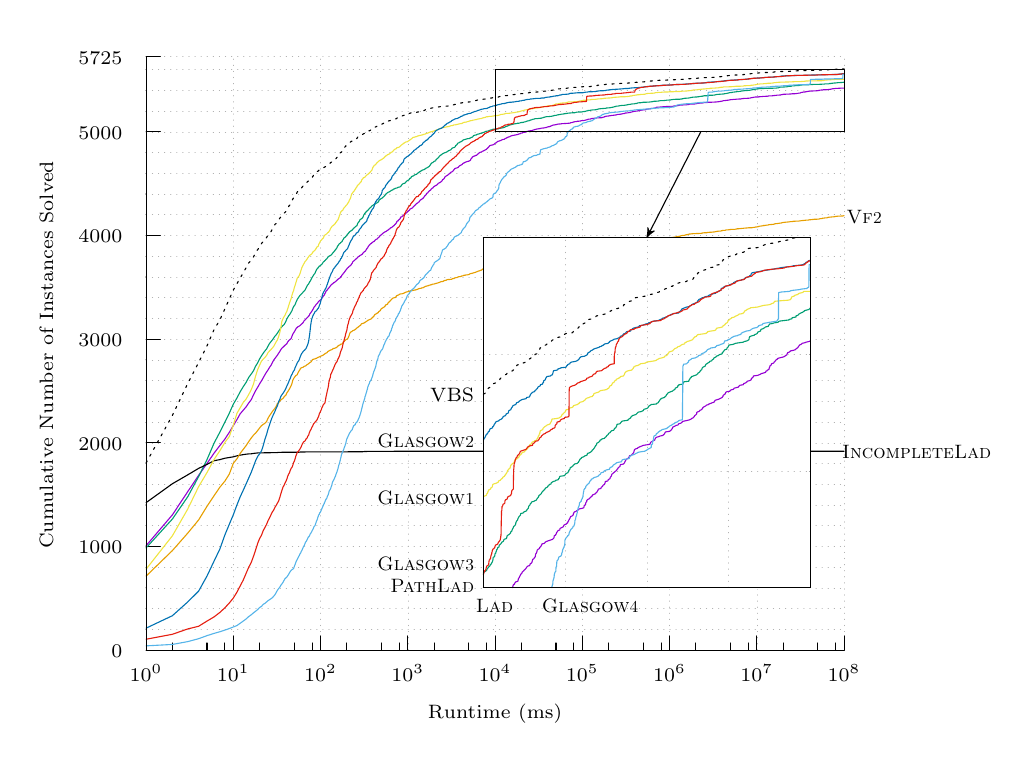
\begin{tikzpicture}[gnuplot]
%% generated with GNUPLOT 5.0p0 (Lua 5.2; terminal rev. 99, script rev. 100)
%% Wed 16 Dec 2015 16:57:53 GMT
\tikzset{every node/.append style={font={\scriptsize}}}
\path (0.000,0.000) rectangle (10.922,8.890);
\gpcolor{color=gp lt color axes}
\gpsetlinetype{gp lt axes}
\gpsetdashtype{gp dt axes}
\gpsetlinewidth{0.50}
\draw[gp path] (1.504,8.521)--(10.368,8.521);
\gpcolor{color=gp lt color border}
\gpsetlinetype{gp lt border}
\gpsetdashtype{gp dt solid}
\gpsetlinewidth{1.00}
\draw[gp path] (1.504,8.521)--(1.684,8.521);
\node[gp node right] at (1.320,8.521) {$5725$};
\gpcolor{color=gp lt color axes}
\gpsetlinetype{gp lt axes}
\gpsetdashtype{gp dt axes}
\gpsetlinewidth{0.50}
\draw[gp path] (1.504,0.985)--(10.368,0.985);
\gpcolor{color=gp lt color border}
\gpsetlinetype{gp lt border}
\gpsetdashtype{gp dt solid}
\gpsetlinewidth{1.00}
\draw[gp path] (1.504,0.985)--(1.684,0.985);
\node[gp node right] at (1.320,0.985) {$0$};
\gpcolor{color=gp lt color axes}
\gpsetlinetype{gp lt axes}
\gpsetdashtype{gp dt axes}
\gpsetlinewidth{0.50}
\draw[gp path] (1.504,1.248)--(10.368,1.248);
\gpcolor{color=gp lt color border}
\gpsetlinetype{gp lt border}
\gpsetdashtype{gp dt solid}
\gpsetlinewidth{1.00}
\draw[gp path] (1.504,1.248)--(1.505,1.248);
\gpcolor{color=gp lt color axes}
\gpsetlinetype{gp lt axes}
\gpsetdashtype{gp dt axes}
\gpsetlinewidth{0.50}
\draw[gp path] (1.504,1.512)--(10.368,1.512);
\gpcolor{color=gp lt color border}
\gpsetlinetype{gp lt border}
\gpsetdashtype{gp dt solid}
\gpsetlinewidth{1.00}
\draw[gp path] (1.504,1.512)--(1.505,1.512);
\gpcolor{color=gp lt color axes}
\gpsetlinetype{gp lt axes}
\gpsetdashtype{gp dt axes}
\gpsetlinewidth{0.50}
\draw[gp path] (1.504,1.775)--(10.368,1.775);
\gpcolor{color=gp lt color border}
\gpsetlinetype{gp lt border}
\gpsetdashtype{gp dt solid}
\gpsetlinewidth{1.00}
\draw[gp path] (1.504,1.775)--(1.505,1.775);
\gpcolor{color=gp lt color axes}
\gpsetlinetype{gp lt axes}
\gpsetdashtype{gp dt axes}
\gpsetlinewidth{0.50}
\draw[gp path] (1.504,2.038)--(10.368,2.038);
\gpcolor{color=gp lt color border}
\gpsetlinetype{gp lt border}
\gpsetdashtype{gp dt solid}
\gpsetlinewidth{1.00}
\draw[gp path] (1.504,2.038)--(1.505,2.038);
\gpcolor{color=gp lt color axes}
\gpsetlinetype{gp lt axes}
\gpsetdashtype{gp dt axes}
\gpsetlinewidth{0.50}
\draw[gp path] (1.504,2.301)--(10.368,2.301);
\gpcolor{color=gp lt color border}
\gpsetlinetype{gp lt border}
\gpsetdashtype{gp dt solid}
\gpsetlinewidth{1.00}
\draw[gp path] (1.504,2.301)--(1.684,2.301);
\node[gp node right] at (1.320,2.301) {$1000$};
\gpcolor{color=gp lt color axes}
\gpsetlinetype{gp lt axes}
\gpsetdashtype{gp dt axes}
\gpsetlinewidth{0.50}
\draw[gp path] (1.504,2.565)--(10.368,2.565);
\gpcolor{color=gp lt color border}
\gpsetlinetype{gp lt border}
\gpsetdashtype{gp dt solid}
\gpsetlinewidth{1.00}
\draw[gp path] (1.504,2.565)--(1.505,2.565);
\gpcolor{color=gp lt color axes}
\gpsetlinetype{gp lt axes}
\gpsetdashtype{gp dt axes}
\gpsetlinewidth{0.50}
\draw[gp path] (1.504,2.828)--(10.368,2.828);
\gpcolor{color=gp lt color border}
\gpsetlinetype{gp lt border}
\gpsetdashtype{gp dt solid}
\gpsetlinewidth{1.00}
\draw[gp path] (1.504,2.828)--(1.505,2.828);
\gpcolor{color=gp lt color axes}
\gpsetlinetype{gp lt axes}
\gpsetdashtype{gp dt axes}
\gpsetlinewidth{0.50}
\draw[gp path] (1.504,3.091)--(10.368,3.091);
\gpcolor{color=gp lt color border}
\gpsetlinetype{gp lt border}
\gpsetdashtype{gp dt solid}
\gpsetlinewidth{1.00}
\draw[gp path] (1.504,3.091)--(1.505,3.091);
\gpcolor{color=gp lt color axes}
\gpsetlinetype{gp lt axes}
\gpsetdashtype{gp dt axes}
\gpsetlinewidth{0.50}
\draw[gp path] (1.504,3.354)--(10.368,3.354);
\gpcolor{color=gp lt color border}
\gpsetlinetype{gp lt border}
\gpsetdashtype{gp dt solid}
\gpsetlinewidth{1.00}
\draw[gp path] (1.504,3.354)--(1.505,3.354);
\gpcolor{color=gp lt color axes}
\gpsetlinetype{gp lt axes}
\gpsetdashtype{gp dt axes}
\gpsetlinewidth{0.50}
\draw[gp path] (1.504,3.618)--(10.368,3.618);
\gpcolor{color=gp lt color border}
\gpsetlinetype{gp lt border}
\gpsetdashtype{gp dt solid}
\gpsetlinewidth{1.00}
\draw[gp path] (1.504,3.618)--(1.684,3.618);
\node[gp node right] at (1.320,3.618) {$2000$};
\gpcolor{color=gp lt color axes}
\gpsetlinetype{gp lt axes}
\gpsetdashtype{gp dt axes}
\gpsetlinewidth{0.50}
\draw[gp path] (1.504,3.881)--(10.368,3.881);
\gpcolor{color=gp lt color border}
\gpsetlinetype{gp lt border}
\gpsetdashtype{gp dt solid}
\gpsetlinewidth{1.00}
\draw[gp path] (1.504,3.881)--(1.505,3.881);
\gpcolor{color=gp lt color axes}
\gpsetlinetype{gp lt axes}
\gpsetdashtype{gp dt axes}
\gpsetlinewidth{0.50}
\draw[gp path] (1.504,4.144)--(10.368,4.144);
\gpcolor{color=gp lt color border}
\gpsetlinetype{gp lt border}
\gpsetdashtype{gp dt solid}
\gpsetlinewidth{1.00}
\draw[gp path] (1.504,4.144)--(1.505,4.144);
\gpcolor{color=gp lt color axes}
\gpsetlinetype{gp lt axes}
\gpsetdashtype{gp dt axes}
\gpsetlinewidth{0.50}
\draw[gp path] (1.504,4.407)--(10.368,4.407);
\gpcolor{color=gp lt color border}
\gpsetlinetype{gp lt border}
\gpsetdashtype{gp dt solid}
\gpsetlinewidth{1.00}
\draw[gp path] (1.504,4.407)--(1.505,4.407);
\gpcolor{color=gp lt color axes}
\gpsetlinetype{gp lt axes}
\gpsetdashtype{gp dt axes}
\gpsetlinewidth{0.50}
\draw[gp path] (1.504,4.671)--(10.368,4.671);
\gpcolor{color=gp lt color border}
\gpsetlinetype{gp lt border}
\gpsetdashtype{gp dt solid}
\gpsetlinewidth{1.00}
\draw[gp path] (1.504,4.671)--(1.505,4.671);
\gpcolor{color=gp lt color axes}
\gpsetlinetype{gp lt axes}
\gpsetdashtype{gp dt axes}
\gpsetlinewidth{0.50}
\draw[gp path] (1.504,4.934)--(10.368,4.934);
\gpcolor{color=gp lt color border}
\gpsetlinetype{gp lt border}
\gpsetdashtype{gp dt solid}
\gpsetlinewidth{1.00}
\draw[gp path] (1.504,4.934)--(1.684,4.934);
\node[gp node right] at (1.320,4.934) {$3000$};
\gpcolor{color=gp lt color axes}
\gpsetlinetype{gp lt axes}
\gpsetdashtype{gp dt axes}
\gpsetlinewidth{0.50}
\draw[gp path] (1.504,5.197)--(10.368,5.197);
\gpcolor{color=gp lt color border}
\gpsetlinetype{gp lt border}
\gpsetdashtype{gp dt solid}
\gpsetlinewidth{1.00}
\draw[gp path] (1.504,5.197)--(1.505,5.197);
\gpcolor{color=gp lt color axes}
\gpsetlinetype{gp lt axes}
\gpsetdashtype{gp dt axes}
\gpsetlinewidth{0.50}
\draw[gp path] (1.504,5.461)--(10.368,5.461);
\gpcolor{color=gp lt color border}
\gpsetlinetype{gp lt border}
\gpsetdashtype{gp dt solid}
\gpsetlinewidth{1.00}
\draw[gp path] (1.504,5.461)--(1.505,5.461);
\gpcolor{color=gp lt color axes}
\gpsetlinetype{gp lt axes}
\gpsetdashtype{gp dt axes}
\gpsetlinewidth{0.50}
\draw[gp path] (1.504,5.724)--(10.368,5.724);
\gpcolor{color=gp lt color border}
\gpsetlinetype{gp lt border}
\gpsetdashtype{gp dt solid}
\gpsetlinewidth{1.00}
\draw[gp path] (1.504,5.724)--(1.505,5.724);
\gpcolor{color=gp lt color axes}
\gpsetlinetype{gp lt axes}
\gpsetdashtype{gp dt axes}
\gpsetlinewidth{0.50}
\draw[gp path] (1.504,5.987)--(10.368,5.987);
\gpcolor{color=gp lt color border}
\gpsetlinetype{gp lt border}
\gpsetdashtype{gp dt solid}
\gpsetlinewidth{1.00}
\draw[gp path] (1.504,5.987)--(1.505,5.987);
\gpcolor{color=gp lt color axes}
\gpsetlinetype{gp lt axes}
\gpsetdashtype{gp dt axes}
\gpsetlinewidth{0.50}
\draw[gp path] (1.504,6.250)--(10.368,6.250);
\gpcolor{color=gp lt color border}
\gpsetlinetype{gp lt border}
\gpsetdashtype{gp dt solid}
\gpsetlinewidth{1.00}
\draw[gp path] (1.504,6.250)--(1.684,6.250);
\node[gp node right] at (1.320,6.250) {$4000$};
\gpcolor{color=gp lt color axes}
\gpsetlinetype{gp lt axes}
\gpsetdashtype{gp dt axes}
\gpsetlinewidth{0.50}
\draw[gp path] (1.504,6.514)--(10.368,6.514);
\gpcolor{color=gp lt color border}
\gpsetlinetype{gp lt border}
\gpsetdashtype{gp dt solid}
\gpsetlinewidth{1.00}
\draw[gp path] (1.504,6.514)--(1.505,6.514);
\gpcolor{color=gp lt color axes}
\gpsetlinetype{gp lt axes}
\gpsetdashtype{gp dt axes}
\gpsetlinewidth{0.50}
\draw[gp path] (1.504,6.777)--(10.368,6.777);
\gpcolor{color=gp lt color border}
\gpsetlinetype{gp lt border}
\gpsetdashtype{gp dt solid}
\gpsetlinewidth{1.00}
\draw[gp path] (1.504,6.777)--(1.505,6.777);
\gpcolor{color=gp lt color axes}
\gpsetlinetype{gp lt axes}
\gpsetdashtype{gp dt axes}
\gpsetlinewidth{0.50}
\draw[gp path] (1.504,7.040)--(10.368,7.040);
\gpcolor{color=gp lt color border}
\gpsetlinetype{gp lt border}
\gpsetdashtype{gp dt solid}
\gpsetlinewidth{1.00}
\draw[gp path] (1.504,7.040)--(1.505,7.040);
\gpcolor{color=gp lt color axes}
\gpsetlinetype{gp lt axes}
\gpsetdashtype{gp dt axes}
\gpsetlinewidth{0.50}
\draw[gp path] (1.504,7.303)--(10.368,7.303);
\gpcolor{color=gp lt color border}
\gpsetlinetype{gp lt border}
\gpsetdashtype{gp dt solid}
\gpsetlinewidth{1.00}
\draw[gp path] (1.504,7.303)--(1.505,7.303);
\gpcolor{color=gp lt color axes}
\gpsetlinetype{gp lt axes}
\gpsetdashtype{gp dt axes}
\gpsetlinewidth{0.50}
\draw[gp path] (1.504,7.567)--(10.368,7.567);
\gpcolor{color=gp lt color border}
\gpsetlinetype{gp lt border}
\gpsetdashtype{gp dt solid}
\gpsetlinewidth{1.00}
\draw[gp path] (1.504,7.567)--(1.684,7.567);
\node[gp node right] at (1.320,7.567) {$5000$};
\gpcolor{color=gp lt color axes}
\gpsetlinetype{gp lt axes}
\gpsetdashtype{gp dt axes}
\gpsetlinewidth{0.50}
\draw[gp path] (1.504,7.830)--(10.368,7.830);
\gpcolor{color=gp lt color border}
\gpsetlinetype{gp lt border}
\gpsetdashtype{gp dt solid}
\gpsetlinewidth{1.00}
\draw[gp path] (1.504,7.830)--(1.505,7.830);
\gpcolor{color=gp lt color axes}
\gpsetlinetype{gp lt axes}
\gpsetdashtype{gp dt axes}
\gpsetlinewidth{0.50}
\draw[gp path] (1.504,8.093)--(10.368,8.093);
\gpcolor{color=gp lt color border}
\gpsetlinetype{gp lt border}
\gpsetdashtype{gp dt solid}
\gpsetlinewidth{1.00}
\draw[gp path] (1.504,8.093)--(1.505,8.093);
\gpcolor{color=gp lt color axes}
\gpsetlinetype{gp lt axes}
\gpsetdashtype{gp dt axes}
\gpsetlinewidth{0.50}
\draw[gp path] (1.504,8.356)--(10.368,8.356);
\gpcolor{color=gp lt color border}
\gpsetlinetype{gp lt border}
\gpsetdashtype{gp dt solid}
\gpsetlinewidth{1.00}
\draw[gp path] (1.504,8.356)--(1.505,8.356);
\gpcolor{color=gp lt color axes}
\gpsetlinetype{gp lt axes}
\gpsetdashtype{gp dt axes}
\gpsetlinewidth{0.50}
\draw[gp path] (1.504,0.985)--(1.504,8.521);
\gpcolor{color=gp lt color border}
\gpsetlinetype{gp lt border}
\gpsetdashtype{gp dt solid}
\gpsetlinewidth{1.00}
\draw[gp path] (1.504,0.985)--(1.504,1.165);
\node[gp node center] at (1.504,0.677) {$10^{0}$};
\draw[gp path] (1.838,0.985)--(1.838,1.075);
\draw[gp path] (2.278,0.985)--(2.278,1.075);
\draw[gp path] (2.505,0.985)--(2.505,1.075);
\gpcolor{color=gp lt color axes}
\gpsetlinetype{gp lt axes}
\gpsetdashtype{gp dt axes}
\gpsetlinewidth{0.50}
\draw[gp path] (2.612,0.985)--(2.612,8.521);
\gpcolor{color=gp lt color border}
\gpsetlinetype{gp lt border}
\gpsetdashtype{gp dt solid}
\gpsetlinewidth{1.00}
\draw[gp path] (2.612,0.985)--(2.612,1.165);
\node[gp node center] at (2.612,0.677) {$10^{1}$};
\draw[gp path] (2.946,0.985)--(2.946,1.075);
\draw[gp path] (3.386,0.985)--(3.386,1.075);
\draw[gp path] (3.613,0.985)--(3.613,1.075);
\gpcolor{color=gp lt color axes}
\gpsetlinetype{gp lt axes}
\gpsetdashtype{gp dt axes}
\gpsetlinewidth{0.50}
\draw[gp path] (3.720,0.985)--(3.720,8.521);
\gpcolor{color=gp lt color border}
\gpsetlinetype{gp lt border}
\gpsetdashtype{gp dt solid}
\gpsetlinewidth{1.00}
\draw[gp path] (3.720,0.985)--(3.720,1.165);
\node[gp node center] at (3.720,0.677) {$10^{2}$};
\draw[gp path] (4.054,0.985)--(4.054,1.075);
\draw[gp path] (4.494,0.985)--(4.494,1.075);
\draw[gp path] (4.721,0.985)--(4.721,1.075);
\gpcolor{color=gp lt color axes}
\gpsetlinetype{gp lt axes}
\gpsetdashtype{gp dt axes}
\gpsetlinewidth{0.50}
\draw[gp path] (4.828,0.985)--(4.828,8.521);
\gpcolor{color=gp lt color border}
\gpsetlinetype{gp lt border}
\gpsetdashtype{gp dt solid}
\gpsetlinewidth{1.00}
\draw[gp path] (4.828,0.985)--(4.828,1.165);
\node[gp node center] at (4.828,0.677) {$10^{3}$};
\draw[gp path] (5.162,0.985)--(5.162,1.075);
\draw[gp path] (5.602,0.985)--(5.602,1.075);
\draw[gp path] (5.829,0.985)--(5.829,1.075);
\gpcolor{color=gp lt color axes}
\gpsetlinetype{gp lt axes}
\gpsetdashtype{gp dt axes}
\gpsetlinewidth{0.50}
\draw[gp path] (5.936,0.985)--(5.936,8.521);
\gpcolor{color=gp lt color border}
\gpsetlinetype{gp lt border}
\gpsetdashtype{gp dt solid}
\gpsetlinewidth{1.00}
\draw[gp path] (5.936,0.985)--(5.936,1.165);
\node[gp node center] at (5.936,0.677) {$10^{4}$};
\draw[gp path] (6.270,0.985)--(6.270,1.075);
\draw[gp path] (6.710,0.985)--(6.710,1.075);
\draw[gp path] (6.937,0.985)--(6.937,1.075);
\gpcolor{color=gp lt color axes}
\gpsetlinetype{gp lt axes}
\gpsetdashtype{gp dt axes}
\gpsetlinewidth{0.50}
\draw[gp path] (7.044,0.985)--(7.044,8.521);
\gpcolor{color=gp lt color border}
\gpsetlinetype{gp lt border}
\gpsetdashtype{gp dt solid}
\gpsetlinewidth{1.00}
\draw[gp path] (7.044,0.985)--(7.044,1.165);
\node[gp node center] at (7.044,0.677) {$10^{5}$};
\draw[gp path] (7.378,0.985)--(7.378,1.075);
\draw[gp path] (7.818,0.985)--(7.818,1.075);
\draw[gp path] (8.045,0.985)--(8.045,1.075);
\gpcolor{color=gp lt color axes}
\gpsetlinetype{gp lt axes}
\gpsetdashtype{gp dt axes}
\gpsetlinewidth{0.50}
\draw[gp path] (8.152,0.985)--(8.152,8.521);
\gpcolor{color=gp lt color border}
\gpsetlinetype{gp lt border}
\gpsetdashtype{gp dt solid}
\gpsetlinewidth{1.00}
\draw[gp path] (8.152,0.985)--(8.152,1.165);
\node[gp node center] at (8.152,0.677) {$10^{6}$};
\draw[gp path] (8.486,0.985)--(8.486,1.075);
\draw[gp path] (8.926,0.985)--(8.926,1.075);
\draw[gp path] (9.153,0.985)--(9.153,1.075);
\gpcolor{color=gp lt color axes}
\gpsetlinetype{gp lt axes}
\gpsetdashtype{gp dt axes}
\gpsetlinewidth{0.50}
\draw[gp path] (9.260,0.985)--(9.260,8.521);
\gpcolor{color=gp lt color border}
\gpsetlinetype{gp lt border}
\gpsetdashtype{gp dt solid}
\gpsetlinewidth{1.00}
\draw[gp path] (9.260,0.985)--(9.260,1.165);
\node[gp node center] at (9.260,0.677) {$10^{7}$};
\draw[gp path] (9.594,0.985)--(9.594,1.075);
\draw[gp path] (10.034,0.985)--(10.034,1.075);
\draw[gp path] (10.261,0.985)--(10.261,1.075);
\gpcolor{color=gp lt color axes}
\gpsetlinetype{gp lt axes}
\gpsetdashtype{gp dt axes}
\gpsetlinewidth{0.50}
\draw[gp path] (10.368,0.985)--(10.368,8.521);
\gpcolor{color=gp lt color border}
\gpsetlinetype{gp lt border}
\gpsetdashtype{gp dt solid}
\gpsetlinewidth{1.00}
\draw[gp path] (10.368,0.985)--(10.368,1.165);
\node[gp node center] at (10.368,0.677) {$10^{8}$};
\draw[gp path] (1.504,8.521)--(1.504,0.985)--(10.368,0.985);
\node[gp node center,rotate=-270] at (0.246,4.753) {Cumulative Number of Instances Solved};
\node[gp node center] at (5.936,0.215) {Runtime (ms)};
\gpcolor{rgb color={0.580,0.000,0.827}}
\draw[gp path] (1.504,2.311)--(1.838,2.703)--(2.033,2.998)--(2.171,3.204)--(2.278,3.356)%
  --(2.366,3.485)--(2.440,3.582)--(2.505,3.666)--(2.561,3.751)--(2.612,3.837)--(2.658,3.913)%
  --(2.700,3.988)--(2.738,4.032)--(2.774,4.074)--(2.807,4.123)--(2.838,4.164)--(2.867,4.224)%
  --(2.895,4.280)--(2.921,4.323)--(2.946,4.367)--(2.969,4.404)--(2.991,4.442)--(3.013,4.482)%
  --(3.033,4.515)--(3.053,4.544)--(3.072,4.576)--(3.090,4.602)--(3.107,4.634)--(3.124,4.667)%
  --(3.141,4.690)--(3.156,4.710)--(3.172,4.731)--(3.187,4.756)--(3.201,4.775)--(3.215,4.801)%
  --(3.228,4.819)--(3.242,4.831)--(3.254,4.843)--(3.267,4.856)--(3.279,4.866)--(3.291,4.876)%
  --(3.303,4.900)--(3.314,4.913)--(3.325,4.925)--(3.336,4.933)--(3.346,4.942)--(3.357,4.973)%
  --(3.367,4.997)--(3.377,5.013)--(3.386,5.027)--(3.396,5.045)--(3.405,5.062)--(3.414,5.076)%
  --(3.423,5.081)--(3.432,5.093)--(3.441,5.095)--(3.450,5.101)--(3.458,5.106)--(3.466,5.113)%
  --(3.474,5.122)--(3.482,5.129)--(3.490,5.135)--(3.498,5.145)--(3.505,5.156)--(3.513,5.172)%
  --(3.520,5.176)--(3.527,5.181)--(3.534,5.192)--(3.541,5.197)--(3.548,5.206)--(3.555,5.212)%
  --(3.562,5.220)--(3.569,5.228)--(3.575,5.233)--(3.582,5.251)--(3.588,5.262)--(3.594,5.268)%
  --(3.600,5.276)--(3.607,5.287)--(3.613,5.295)--(3.619,5.308)--(3.625,5.314)--(3.630,5.326)%
  --(3.636,5.338)--(3.642,5.346)--(3.647,5.351)--(3.653,5.359)--(3.658,5.367)--(3.664,5.374)%
  --(3.669,5.379)--(3.675,5.385)--(3.680,5.392)--(3.685,5.395)--(3.690,5.408)--(3.695,5.413)%
  --(3.700,5.417)--(3.705,5.420)--(3.710,5.426)--(3.715,5.429)--(3.720,5.433)--(3.725,5.436)%
  --(3.730,5.441)--(3.734,5.446)--(3.739,5.462)--(3.743,5.468)--(3.748,5.474)--(3.753,5.478)%
  --(3.757,5.484)--(3.761,5.487)--(3.766,5.493)--(3.770,5.501)--(3.775,5.516)--(3.779,5.518)%
  --(3.783,5.528)--(3.787,5.537)--(3.791,5.546)--(3.796,5.550)--(3.804,5.558)--(3.808,5.563)%
  --(3.812,5.570)--(3.816,5.576)--(3.820,5.578)--(3.824,5.582)--(3.827,5.588)--(3.831,5.595)%
  --(3.835,5.596)--(3.839,5.603)--(3.843,5.608)--(3.846,5.613)--(3.850,5.616)--(3.854,5.622)%
  --(3.857,5.629)--(3.861,5.630)--(3.864,5.633)--(3.868,5.634)--(3.871,5.637)--(3.875,5.638)%
  --(3.878,5.640)--(3.882,5.646)--(3.885,5.650)--(3.892,5.651)--(3.895,5.655)--(3.899,5.658)%
  --(3.905,5.661)--(3.909,5.666)--(3.915,5.669)--(3.918,5.672)--(3.921,5.676)--(3.925,5.680)%
  --(3.928,5.683)--(3.931,5.684)--(3.934,5.690)--(3.940,5.694)--(3.943,5.697)--(3.949,5.701)%
  --(3.952,5.703)--(3.955,5.704)--(3.958,5.707)--(3.961,5.708)--(3.964,5.711)--(3.967,5.712)%
  --(3.970,5.716)--(3.972,5.721)--(3.975,5.726)--(3.978,5.728)--(3.981,5.729)--(3.984,5.732)%
  --(3.987,5.737)--(3.989,5.744)--(3.992,5.749)--(3.995,5.751)--(4.000,5.754)--(4.003,5.761)%
  --(4.006,5.765)--(4.008,5.770)--(4.011,5.772)--(4.013,5.774)--(4.016,5.775)--(4.019,5.778)%
  --(4.021,5.783)--(4.024,5.786)--(4.026,5.791)--(4.029,5.794)--(4.031,5.798)--(4.034,5.800)%
  --(4.036,5.803)--(4.039,5.805)--(4.041,5.812)--(4.044,5.815)--(4.049,5.819)--(4.051,5.823)%
  --(4.054,5.826)--(4.056,5.832)--(4.058,5.834)--(4.061,5.836)--(4.063,5.838)--(4.068,5.841)%
  --(4.070,5.844)--(4.072,5.845)--(4.075,5.846)--(4.077,5.851)--(4.079,5.853)--(4.082,5.857)%
  --(4.084,5.858)--(4.086,5.861)--(4.091,5.862)--(4.093,5.865)--(4.095,5.866)--(4.097,5.867)%
  --(4.099,5.869)--(4.102,5.874)--(4.106,5.875)--(4.108,5.876)--(4.110,5.882)--(4.112,5.887)%
  --(4.114,5.890)--(4.119,5.894)--(4.121,5.899)--(4.123,5.903)--(4.125,5.907)--(4.127,5.912)%
  --(4.129,5.915)--(4.131,5.919)--(4.133,5.920)--(4.135,5.923)--(4.139,5.925)--(4.141,5.928)%
  --(4.145,5.929)--(4.147,5.932)--(4.149,5.934)--(4.155,5.940)--(4.157,5.941)--(4.159,5.944)%
  --(4.161,5.945)--(4.163,5.948)--(4.165,5.949)--(4.169,5.950)--(4.170,5.952)--(4.172,5.954)%
  --(4.174,5.957)--(4.176,5.958)--(4.180,5.962)--(4.183,5.963)--(4.185,5.966)--(4.187,5.967)%
  --(4.189,5.969)--(4.191,5.970)--(4.193,5.973)--(4.194,5.975)--(4.196,5.980)--(4.198,5.982)%
  --(4.200,5.983)--(4.207,5.986)--(4.210,5.988)--(4.212,5.991)--(4.214,5.992)--(4.215,5.994)%
  --(4.219,5.995)--(4.221,5.996)--(4.222,5.998)--(4.224,5.999)--(4.227,6.000)--(4.232,6.002)%
  --(4.234,6.003)--(4.236,6.005)--(4.239,6.007)--(4.241,6.009)--(4.242,6.011)--(4.245,6.012)%
  --(4.250,6.013)--(4.252,6.016)--(4.253,6.019)--(4.255,6.023)--(4.257,6.024)--(4.258,6.025)%
  --(4.260,6.027)--(4.261,6.031)--(4.263,6.032)--(4.264,6.033)--(4.266,6.037)--(4.271,6.038)%
  --(4.272,6.040)--(4.274,6.041)--(4.275,6.044)--(4.277,6.045)--(4.278,6.046)--(4.280,6.048)%
  --(4.283,6.050)--(4.289,6.052)--(4.292,6.056)--(4.293,6.057)--(4.295,6.058)--(4.296,6.065)%
  --(4.297,6.067)--(4.299,6.070)--(4.302,6.074)--(4.303,6.075)--(4.305,6.078)--(4.306,6.081)%
  --(4.307,6.083)--(4.309,6.086)--(4.310,6.088)--(4.312,6.090)--(4.315,6.091)--(4.316,6.092)%
  --(4.317,6.094)--(4.319,6.096)--(4.320,6.099)--(4.321,6.103)--(4.323,6.106)--(4.324,6.107)%
  --(4.326,6.111)--(4.327,6.112)--(4.328,6.115)--(4.331,6.119)--(4.332,6.120)--(4.334,6.121)%
  --(4.335,6.123)--(4.336,6.125)--(4.338,6.128)--(4.339,6.129)--(4.340,6.131)--(4.343,6.132)%
  --(4.346,6.134)--(4.347,6.138)--(4.348,6.140)--(4.351,6.141)--(4.353,6.142)--(4.355,6.144)%
  --(4.359,6.148)--(4.362,6.149)--(4.367,6.150)--(4.369,6.153)--(4.370,6.157)--(4.371,6.158)%
  --(4.372,6.160)--(4.375,6.161)--(4.379,6.162)--(4.381,6.165)--(4.382,6.167)--(4.387,6.169)%
  --(4.388,6.170)--(4.389,6.171)--(4.394,6.173)--(4.397,6.174)--(4.398,6.175)--(4.402,6.177)%
  --(4.404,6.181)--(4.405,6.182)--(4.406,6.183)--(4.407,6.185)--(4.409,6.187)--(4.411,6.188)%
  --(4.412,6.191)--(4.414,6.192)--(4.415,6.195)--(4.417,6.196)--(4.420,6.198)--(4.421,6.199)%
  --(4.423,6.200)--(4.430,6.203)--(4.432,6.204)--(4.437,6.206)--(4.441,6.208)--(4.443,6.211)%
  --(4.444,6.212)--(4.445,6.213)--(4.447,6.215)--(4.448,6.219)--(4.450,6.220)--(4.452,6.223)%
  --(4.453,6.224)--(4.454,6.225)--(4.459,6.228)--(4.460,6.229)--(4.463,6.231)--(4.465,6.232)%
  --(4.466,6.233)--(4.467,6.235)--(4.468,6.236)--(4.469,6.237)--(4.470,6.240)--(4.471,6.242)%
  --(4.472,6.245)--(4.473,6.246)--(4.475,6.249)--(4.481,6.250)--(4.482,6.252)--(4.483,6.254)%
  --(4.485,6.256)--(4.486,6.258)--(4.491,6.260)--(4.492,6.261)--(4.496,6.263)--(4.498,6.265)%
  --(4.499,6.266)--(4.501,6.267)--(4.502,6.269)--(4.503,6.270)--(4.504,6.271)--(4.505,6.273)%
  --(4.507,6.274)--(4.508,6.275)--(4.509,6.277)--(4.511,6.278)--(4.515,6.281)--(4.518,6.282)%
  --(4.519,6.283)--(4.523,6.287)--(4.527,6.289)--(4.529,6.290)--(4.530,6.291)--(4.531,6.294)%
  --(4.534,6.295)--(4.542,6.296)--(4.544,6.299)--(4.547,6.300)--(4.551,6.302)--(4.557,6.304)%
  --(4.558,6.307)--(4.560,6.308)--(4.561,6.310)--(4.563,6.311)--(4.564,6.312)--(4.567,6.314)%
  --(4.569,6.316)--(4.575,6.317)--(4.576,6.319)--(4.577,6.320)--(4.578,6.321)--(4.580,6.324)%
  --(4.581,6.325)--(4.582,6.327)--(4.586,6.328)--(4.587,6.329)--(4.590,6.331)--(4.592,6.332)%
  --(4.593,6.335)--(4.599,6.336)--(4.600,6.337)--(4.603,6.339)--(4.604,6.344)--(4.606,6.345)%
  --(4.606,6.346)--(4.609,6.348)--(4.611,6.349)--(4.620,6.350)--(4.621,6.352)--(4.623,6.353)%
  --(4.624,6.354)--(4.626,6.356)--(4.627,6.357)--(4.628,6.360)--(4.635,6.361)--(4.635,6.362)%
  --(4.636,6.365)--(4.637,6.366)--(4.639,6.367)--(4.641,6.369)--(4.642,6.370)--(4.644,6.371)%
  --(4.648,6.373)--(4.649,6.374)--(4.650,6.375)--(4.653,6.377)--(4.656,6.378)--(4.657,6.382)%
  --(4.658,6.385)--(4.658,6.386)--(4.660,6.387)--(4.661,6.389)--(4.663,6.390)--(4.664,6.391)%
  --(4.669,6.392)--(4.669,6.394)--(4.670,6.395)--(4.671,6.396)--(4.671,6.398)--(4.675,6.400)%
  --(4.677,6.402)--(4.677,6.404)--(4.678,6.406)--(4.679,6.407)--(4.679,6.408)--(4.682,6.410)%
  --(4.684,6.411)--(4.684,6.414)--(4.685,6.415)--(4.686,6.418)--(4.686,6.421)--(4.688,6.423)%
  --(4.690,6.424)--(4.691,6.428)--(4.691,6.432)--(4.693,6.433)--(4.693,6.435)--(4.704,6.436)%
  --(4.706,6.437)--(4.707,6.439)--(4.708,6.440)--(4.709,6.444)--(4.710,6.446)--(4.711,6.449)%
  --(4.713,6.450)--(4.719,6.452)--(4.720,6.453)--(4.721,6.454)--(4.722,6.456)--(4.723,6.457)%
  --(4.724,6.458)--(4.726,6.461)--(4.727,6.462)--(4.728,6.465)--(4.729,6.468)--(4.732,6.469)%
  --(4.733,6.470)--(4.733,6.471)--(4.734,6.474)--(4.735,6.477)--(4.737,6.481)--(4.738,6.483)%
  --(4.738,6.485)--(4.743,6.486)--(4.745,6.487)--(4.753,6.489)--(4.754,6.491)--(4.754,6.493)%
  --(4.757,6.496)--(4.762,6.498)--(4.763,6.500)--(4.764,6.502)--(4.766,6.503)--(4.767,6.504)%
  --(4.768,6.506)--(4.769,6.507)--(4.770,6.508)--(4.772,6.511)--(4.783,6.512)--(4.783,6.514)%
  --(4.784,6.515)--(4.789,6.516)--(4.789,6.518)--(4.790,6.519)--(4.792,6.520)--(4.794,6.521)%
  --(4.794,6.524)--(4.795,6.525)--(4.796,6.527)--(4.797,6.528)--(4.798,6.529)--(4.800,6.531)%
  --(4.801,6.532)--(4.804,6.533)--(4.807,6.536)--(4.809,6.537)--(4.810,6.539)--(4.812,6.540)%
  --(4.814,6.541)--(4.816,6.543)--(4.819,6.545)--(4.820,6.547)--(4.821,6.548)--(4.821,6.550)%
  --(4.822,6.552)--(4.823,6.553)--(4.823,6.554)--(4.826,6.556)--(4.827,6.557)--(4.829,6.558)%
  --(4.832,6.560)--(4.833,6.562)--(4.837,6.564)--(4.838,6.566)--(4.840,6.568)--(4.843,6.569)%
  --(4.848,6.570)--(4.849,6.572)--(4.850,6.573)--(4.851,6.574)--(4.851,6.577)--(4.851,6.578)%
  --(4.852,6.579)--(4.853,6.583)--(4.855,6.586)--(4.856,6.587)--(4.861,6.589)--(4.865,6.590)%
  --(4.868,6.591)--(4.869,6.593)--(4.869,6.594)--(4.873,6.595)--(4.876,6.597)--(4.882,6.598)%
  --(4.883,6.599)--(4.886,6.600)--(4.886,6.602)--(4.889,6.604)--(4.891,6.606)--(4.893,6.608)%
  --(4.893,6.610)--(4.894,6.611)--(4.896,6.612)--(4.897,6.614)--(4.897,6.615)--(4.901,6.616)%
  --(4.902,6.619)--(4.904,6.620)--(4.906,6.623)--(4.907,6.624)--(4.909,6.625)--(4.911,6.627)%
  --(4.913,6.629)--(4.913,6.631)--(4.914,6.632)--(4.915,6.633)--(4.917,6.635)--(4.921,6.636)%
  --(4.921,6.637)--(4.925,6.640)--(4.926,6.641)--(4.926,6.643)--(4.927,6.644)--(4.927,6.645)%
  --(4.928,6.647)--(4.931,6.648)--(4.932,6.649)--(4.933,6.650)--(4.938,6.652)--(4.939,6.653)%
  --(4.940,6.656)--(4.941,6.657)--(4.943,6.658)--(4.944,6.660)--(4.950,6.661)--(4.950,6.662)%
  --(4.954,6.665)--(4.955,6.666)--(4.955,6.668)--(4.958,6.669)--(4.958,6.670)--(4.960,6.672)%
  --(4.963,6.673)--(4.964,6.674)--(4.966,6.676)--(4.971,6.677)--(4.972,6.678)--(4.973,6.679)%
  --(4.973,6.681)--(4.974,6.682)--(4.976,6.685)--(4.976,6.686)--(4.977,6.689)--(4.979,6.690)%
  --(4.980,6.691)--(4.981,6.693)--(4.982,6.694)--(4.983,6.695)--(4.984,6.697)--(4.986,6.698)%
  --(4.986,6.699)--(4.987,6.701)--(4.989,6.702)--(4.991,6.703)--(4.994,6.704)--(4.996,6.706)%
  --(4.998,6.707)--(5.000,6.708)--(5.004,6.710)--(5.005,6.711)--(5.005,6.712)--(5.007,6.714)%
  --(5.011,6.716)--(5.012,6.718)--(5.016,6.719)--(5.019,6.720)--(5.019,6.722)--(5.020,6.723)%
  --(5.022,6.724)--(5.023,6.726)--(5.025,6.728)--(5.026,6.729)--(5.026,6.731)--(5.030,6.735)%
  --(5.031,6.736)--(5.032,6.737)--(5.034,6.740)--(5.036,6.743)--(5.037,6.744)--(5.039,6.745)%
  --(5.039,6.747)--(5.040,6.748)--(5.040,6.749)--(5.041,6.751)--(5.043,6.754)--(5.045,6.756)%
  --(5.048,6.757)--(5.049,6.758)--(5.051,6.760)--(5.053,6.761)--(5.054,6.762)--(5.054,6.764)%
  --(5.057,6.765)--(5.058,6.768)--(5.059,6.769)--(5.059,6.770)--(5.060,6.772)--(5.060,6.773)%
  --(5.061,6.774)--(5.064,6.776)--(5.064,6.777)--(5.065,6.778)--(5.065,6.779)--(5.066,6.781)%
  --(5.067,6.783)--(5.067,6.785)--(5.069,6.786)--(5.069,6.787)--(5.071,6.789)--(5.078,6.790)%
  --(5.082,6.791)--(5.082,6.794)--(5.083,6.797)--(5.084,6.798)--(5.085,6.799)--(5.087,6.801)%
  --(5.087,6.802)--(5.088,6.803)--(5.088,6.805)--(5.088,6.806)--(5.090,6.807)--(5.092,6.808)%
  --(5.093,6.811)--(5.097,6.812)--(5.098,6.814)--(5.100,6.815)--(5.102,6.816)--(5.103,6.818)%
  --(5.103,6.819)--(5.104,6.820)--(5.106,6.822)--(5.106,6.823)--(5.111,6.824)--(5.115,6.826)%
  --(5.116,6.827)--(5.117,6.828)--(5.117,6.830)--(5.119,6.831)--(5.121,6.832)--(5.121,6.836)%
  --(5.122,6.837)--(5.122,6.839)--(5.125,6.840)--(5.130,6.843)--(5.131,6.844)--(5.131,6.845)%
  --(5.132,6.847)--(5.134,6.848)--(5.134,6.849)--(5.136,6.852)--(5.146,6.853)--(5.146,6.855)%
  --(5.147,6.857)--(5.147,6.858)--(5.148,6.860)--(5.149,6.861)--(5.149,6.862)--(5.154,6.864)%
  --(5.155,6.865)--(5.156,6.866)--(5.156,6.870)--(5.163,6.873)--(5.165,6.874)--(5.166,6.876)%
  --(5.168,6.877)--(5.171,6.880)--(5.174,6.881)--(5.177,6.882)--(5.178,6.883)--(5.181,6.885)%
  --(5.186,6.886)--(5.187,6.887)--(5.189,6.889)--(5.189,6.890)--(5.192,6.891)--(5.194,6.893)%
  --(5.197,6.894)--(5.199,6.895)--(5.201,6.897)--(5.203,6.898)--(5.204,6.899)--(5.206,6.901)%
  --(5.206,6.902)--(5.208,6.903)--(5.210,6.906)--(5.210,6.907)--(5.211,6.908)--(5.211,6.910)%
  --(5.214,6.912)--(5.217,6.915)--(5.225,6.916)--(5.226,6.918)--(5.226,6.919)--(5.227,6.920)%
  --(5.232,6.922)--(5.236,6.923)--(5.239,6.924)--(5.239,6.926)--(5.240,6.927)--(5.241,6.928)%
  --(5.245,6.930)--(5.246,6.931)--(5.250,6.932)--(5.251,6.935)--(5.251,6.936)--(5.255,6.937)%
  --(5.255,6.939)--(5.259,6.941)--(5.260,6.943)--(5.261,6.944)--(5.262,6.945)--(5.263,6.947)%
  --(5.263,6.948)--(5.264,6.949)--(5.265,6.952)--(5.265,6.953)--(5.267,6.955)--(5.268,6.956)%
  --(5.268,6.957)--(5.269,6.959)--(5.270,6.960)--(5.275,6.962)--(5.277,6.964)--(5.278,6.965)%
  --(5.281,6.966)--(5.282,6.968)--(5.283,6.969)--(5.284,6.970)--(5.286,6.972)--(5.289,6.973)%
  --(5.290,6.974)--(5.291,6.976)--(5.292,6.977)--(5.292,6.978)--(5.293,6.981)--(5.294,6.982)%
  --(5.294,6.984)--(5.294,6.985)--(5.294,6.986)--(5.296,6.987)--(5.297,6.989)--(5.298,6.990)%
  --(5.299,6.993)--(5.300,6.994)--(5.301,6.995)--(5.302,6.997)--(5.305,6.998)--(5.306,6.999)%
  --(5.308,7.001)--(5.310,7.002)--(5.312,7.003)--(5.312,7.005)--(5.314,7.006)--(5.315,7.007)%
  --(5.318,7.009)--(5.323,7.010)--(5.326,7.011)--(5.327,7.012)--(5.329,7.014)--(5.331,7.015)%
  --(5.332,7.016)--(5.333,7.018)--(5.338,7.019)--(5.338,7.020)--(5.339,7.022)--(5.340,7.023)%
  --(5.341,7.024)--(5.341,7.026)--(5.347,7.027)--(5.347,7.028)--(5.350,7.030)--(5.352,7.031)%
  --(5.352,7.032)--(5.353,7.034)--(5.353,7.035)--(5.354,7.036)--(5.355,7.037)--(5.361,7.039)%
  --(5.361,7.040)--(5.363,7.041)--(5.365,7.043)--(5.366,7.044)--(5.368,7.047)--(5.369,7.049)%
  --(5.372,7.052)--(5.374,7.053)--(5.378,7.055)--(5.379,7.056)--(5.384,7.057)--(5.385,7.059)%
  --(5.389,7.060)--(5.392,7.061)--(5.392,7.063)--(5.393,7.064)--(5.396,7.065)--(5.399,7.066)%
  --(5.400,7.068)--(5.400,7.069)--(5.402,7.070)--(5.403,7.072)--(5.404,7.073)--(5.405,7.074)%
  --(5.405,7.076)--(5.409,7.078)--(5.409,7.080)--(5.410,7.081)--(5.411,7.082)--(5.412,7.084)%
  --(5.413,7.085)--(5.414,7.086)--(5.416,7.088)--(5.416,7.089)--(5.417,7.090)--(5.418,7.091)%
  --(5.419,7.093)--(5.420,7.094)--(5.421,7.095)--(5.422,7.097)--(5.424,7.098)--(5.424,7.099)%
  --(5.426,7.101)--(5.432,7.102)--(5.435,7.103)--(5.436,7.105)--(5.439,7.106)--(5.450,7.107)%
  --(5.451,7.109)--(5.451,7.110)--(5.454,7.111)--(5.460,7.113)--(5.464,7.114)--(5.464,7.115)%
  --(5.468,7.116)--(5.470,7.118)--(5.471,7.119)--(5.471,7.120)--(5.471,7.122)--(5.473,7.123)%
  --(5.474,7.124)--(5.475,7.126)--(5.478,7.127)--(5.478,7.128)--(5.478,7.130)--(5.478,7.131)%
  --(5.481,7.132)--(5.482,7.134)--(5.484,7.135)--(5.485,7.136)--(5.489,7.138)--(5.491,7.139)%
  --(5.496,7.140)--(5.497,7.141)--(5.497,7.143)--(5.497,7.144)--(5.505,7.145)--(5.506,7.147)%
  --(5.511,7.148)--(5.512,7.149)--(5.512,7.151)--(5.517,7.152)--(5.518,7.153)--(5.519,7.155)%
  --(5.521,7.157)--(5.522,7.159)--(5.523,7.160)--(5.524,7.161)--(5.525,7.163)--(5.528,7.164)%
  --(5.528,7.166)--(5.533,7.168)--(5.533,7.169)--(5.541,7.170)--(5.543,7.172)--(5.544,7.173)%
  --(5.544,7.174)--(5.545,7.176)--(5.548,7.177)--(5.551,7.178)--(5.558,7.180)--(5.560,7.181)%
  --(5.561,7.182)--(5.565,7.184)--(5.568,7.185)--(5.572,7.186)--(5.577,7.188)--(5.581,7.189)%
  --(5.584,7.190)--(5.592,7.192)--(5.596,7.193)--(5.601,7.194)--(5.602,7.195)--(5.607,7.197)%
  --(5.610,7.198)--(5.613,7.199)--(5.614,7.201)--(5.618,7.202)--(5.619,7.203)--(5.621,7.205)%
  --(5.623,7.206)--(5.623,7.207)--(5.624,7.209)--(5.624,7.210)--(5.626,7.211)--(5.626,7.214)%
  --(5.626,7.215)--(5.627,7.217)--(5.627,7.218)--(5.627,7.219)--(5.628,7.220)--(5.629,7.222)%
  --(5.629,7.223)--(5.629,7.224)--(5.632,7.226)--(5.633,7.227)--(5.634,7.228)--(5.635,7.230)%
  --(5.636,7.231)--(5.638,7.232)--(5.639,7.234)--(5.639,7.235)--(5.642,7.236)--(5.643,7.238)%
  --(5.643,7.239)--(5.644,7.240)--(5.644,7.242)--(5.645,7.243)--(5.646,7.244)--(5.647,7.245)%
  --(5.647,7.247)--(5.651,7.248)--(5.653,7.249)--(5.655,7.251)--(5.656,7.252)--(5.657,7.253)%
  --(5.662,7.255)--(5.665,7.256)--(5.666,7.257)--(5.667,7.259)--(5.671,7.260)--(5.680,7.261)%
  --(5.685,7.263)--(5.686,7.264)--(5.687,7.267)--(5.692,7.268)--(5.694,7.269)--(5.703,7.270)%
  --(5.704,7.272)--(5.707,7.273)--(5.707,7.274)--(5.708,7.276)--(5.708,7.277)--(5.710,7.278)%
  --(5.710,7.280)--(5.714,7.281)--(5.715,7.282)--(5.716,7.284)--(5.719,7.285)--(5.720,7.286)%
  --(5.721,7.288)--(5.721,7.289)--(5.722,7.290)--(5.722,7.292)--(5.728,7.293)--(5.729,7.294)%
  --(5.731,7.295)--(5.732,7.297)--(5.733,7.298)--(5.734,7.299)--(5.735,7.301)--(5.735,7.302)%
  --(5.737,7.303)--(5.738,7.305)--(5.738,7.306)--(5.748,7.307)--(5.752,7.309)--(5.759,7.310)%
  --(5.761,7.311)--(5.763,7.313)--(5.768,7.314)--(5.770,7.315)--(5.770,7.317)--(5.771,7.318)%
  --(5.774,7.319)--(5.777,7.321)--(5.779,7.322)--(5.783,7.323)--(5.787,7.324)--(5.790,7.326)%
  --(5.790,7.327)--(5.799,7.328)--(5.800,7.330)--(5.802,7.331)--(5.803,7.332)--(5.805,7.334)%
  --(5.808,7.335)--(5.810,7.336)--(5.811,7.338)--(5.814,7.339)--(5.815,7.340)--(5.818,7.342)%
  --(5.824,7.343)--(5.825,7.344)--(5.826,7.346)--(5.826,7.347)--(5.828,7.348)--(5.828,7.349)%
  --(5.829,7.351)--(5.829,7.352)--(5.836,7.353)--(5.838,7.355)--(5.838,7.356)--(5.839,7.357)%
  --(5.839,7.359)--(5.841,7.360)--(5.841,7.361)--(5.844,7.363)--(5.845,7.364)--(5.846,7.365)%
  --(5.850,7.367)--(5.850,7.368)--(5.850,7.369)--(5.852,7.371)--(5.852,7.372)--(5.855,7.373)%
  --(5.856,7.374)--(5.856,7.376)--(5.857,7.377)--(5.858,7.378)--(5.860,7.380)--(5.862,7.381)%
  --(5.862,7.382)--(5.863,7.384)--(5.863,7.385)--(5.864,7.386)--(5.866,7.388)--(5.867,7.389)%
  --(5.868,7.390)--(5.869,7.392)--(5.874,7.393)--(5.875,7.394)--(5.884,7.396)--(5.887,7.397)%
  --(5.892,7.398)--(5.896,7.399)--(5.905,7.401)--(5.905,7.402)--(5.912,7.403)--(5.916,7.405)%
  --(5.919,7.406)--(5.920,7.407)--(5.924,7.409)--(5.925,7.410)--(5.927,7.411)--(5.928,7.413)%
  --(5.929,7.414)--(5.931,7.415)--(5.932,7.417)--(5.933,7.418)--(5.933,7.419)--(5.936,7.421)%
  --(5.937,7.422)--(5.937,7.423)--(5.940,7.424)--(5.942,7.426)--(5.952,7.428)--(5.952,7.430)%
  --(5.953,7.431)--(5.954,7.432)--(5.954,7.434)--(5.958,7.435)--(5.960,7.436)--(5.961,7.438)%
  --(5.962,7.439)--(5.966,7.440)--(5.966,7.442)--(5.968,7.443)--(5.968,7.444)--(5.970,7.446)%
  --(5.974,7.447)--(5.979,7.448)--(5.988,7.450)--(5.991,7.451)--(5.994,7.452)--(5.995,7.453)%
  --(5.996,7.455)--(6.004,7.456)--(6.009,7.457)--(6.012,7.459)--(6.013,7.460)--(6.016,7.461)%
  --(6.017,7.463)--(6.020,7.464)--(6.021,7.465)--(6.025,7.467)--(6.027,7.468)--(6.036,7.469)%
  --(6.038,7.471)--(6.050,7.472)--(6.054,7.473)--(6.057,7.475)--(6.058,7.476)--(6.059,7.477)%
  --(6.059,7.478)--(6.061,7.480)--(6.065,7.481)--(6.066,7.482)--(6.074,7.484)--(6.074,7.485)%
  --(6.078,7.486)--(6.079,7.488)--(6.081,7.489)--(6.085,7.490)--(6.088,7.492)--(6.089,7.493)%
  --(6.089,7.494)--(6.091,7.496)--(6.092,7.497)--(6.099,7.498)--(6.101,7.500)--(6.105,7.501)%
  --(6.111,7.502)--(6.118,7.503)--(6.120,7.505)--(6.123,7.506)--(6.125,7.507)--(6.128,7.509)%
  --(6.130,7.510)--(6.131,7.511)--(6.134,7.513)--(6.135,7.514)--(6.141,7.515)--(6.146,7.517)%
  --(6.146,7.518)--(6.152,7.519)--(6.159,7.521)--(6.168,7.522)--(6.175,7.523)--(6.181,7.525)%
  --(6.182,7.526)--(6.189,7.527)--(6.203,7.528)--(6.204,7.530)--(6.209,7.531)--(6.219,7.532)%
  --(6.222,7.534)--(6.223,7.535)--(6.231,7.536)--(6.238,7.538)--(6.238,7.539)--(6.240,7.540)%
  --(6.250,7.542)--(6.254,7.543)--(6.254,7.544)--(6.258,7.546)--(6.260,7.547)--(6.260,7.548)%
  --(6.262,7.550)--(6.268,7.551)--(6.281,7.552)--(6.281,7.553)--(6.282,7.555)--(6.288,7.556)%
  --(6.288,7.557)--(6.291,7.559)--(6.301,7.560)--(6.317,7.561)--(6.318,7.563)--(6.326,7.564)%
  --(6.330,7.565)--(6.333,7.567)--(6.334,7.568)--(6.335,7.569)--(6.336,7.571)--(6.340,7.572)%
  --(6.343,7.573)--(6.357,7.575)--(6.358,7.576)--(6.361,7.577)--(6.370,7.579)--(6.374,7.580)%
  --(6.402,7.581)--(6.405,7.582)--(6.407,7.584)--(6.408,7.585)--(6.410,7.586)--(6.412,7.588)%
  --(6.422,7.589)--(6.423,7.590)--(6.426,7.592)--(6.432,7.593)--(6.436,7.594)--(6.438,7.596)%
  --(6.445,7.597)--(6.448,7.598)--(6.459,7.600)--(6.461,7.601)--(6.464,7.602)--(6.472,7.604)%
  --(6.484,7.605)--(6.488,7.606)--(6.500,7.607)--(6.504,7.609)--(6.514,7.610)--(6.518,7.611)%
  --(6.521,7.613)--(6.529,7.614)--(6.539,7.615)--(6.563,7.617)--(6.565,7.618)--(6.570,7.619)%
  --(6.571,7.621)--(6.585,7.622)--(6.590,7.623)--(6.595,7.625)--(6.596,7.626)--(6.599,7.627)%
  --(6.602,7.629)--(6.604,7.630)--(6.610,7.631)--(6.624,7.632)--(6.625,7.634)--(6.633,7.635)%
  --(6.639,7.636)--(6.640,7.638)--(6.640,7.639)--(6.643,7.640)--(6.644,7.642)--(6.645,7.643)%
  --(6.654,7.644)--(6.656,7.646)--(6.660,7.647)--(6.663,7.648)--(6.664,7.650)--(6.664,7.651)%
  --(6.670,7.652)--(6.680,7.654)--(6.695,7.655)--(6.698,7.656)--(6.699,7.657)--(6.710,7.659)%
  --(6.713,7.660)--(6.723,7.661)--(6.724,7.663)--(6.729,7.664)--(6.730,7.665)--(6.764,7.667)%
  --(6.768,7.668)--(6.775,7.669)--(6.786,7.671)--(6.809,7.672)--(6.832,7.673)--(6.853,7.675)%
  --(6.876,7.676)--(6.882,7.677)--(6.891,7.679)--(6.894,7.680)--(6.894,7.681)--(6.896,7.682)%
  --(6.897,7.684)--(6.913,7.685)--(6.914,7.686)--(6.923,7.688)--(6.926,7.689)--(6.927,7.690)%
  --(6.931,7.692)--(6.943,7.693)--(6.944,7.694)--(6.947,7.696)--(6.973,7.697)--(6.973,7.698)%
  --(6.974,7.700)--(6.980,7.701)--(6.997,7.702)--(7.015,7.704)--(7.023,7.705)--(7.025,7.706)%
  --(7.028,7.708)--(7.037,7.709)--(7.061,7.710)--(7.061,7.711)--(7.079,7.713)--(7.080,7.714)%
  --(7.081,7.715)--(7.089,7.717)--(7.091,7.718)--(7.095,7.719)--(7.103,7.721)--(7.104,7.722)%
  --(7.110,7.723)--(7.112,7.725)--(7.115,7.726)--(7.119,7.727)--(7.139,7.729)--(7.149,7.730)%
  --(7.154,7.731)--(7.155,7.733)--(7.157,7.734)--(7.163,7.735)--(7.164,7.736)--(7.172,7.738)%
  --(7.193,7.739)--(7.201,7.740)--(7.218,7.742)--(7.226,7.743)--(7.234,7.744)--(7.272,7.746)%
  --(7.298,7.747)--(7.298,7.748)--(7.302,7.750)--(7.303,7.751)--(7.304,7.752)--(7.320,7.754)%
  --(7.321,7.755)--(7.322,7.756)--(7.323,7.758)--(7.327,7.759)--(7.333,7.760)--(7.337,7.761)%
  --(7.338,7.763)--(7.341,7.764)--(7.346,7.765)--(7.365,7.767)--(7.376,7.768)--(7.381,7.769)%
  --(7.389,7.771)--(7.399,7.772)--(7.408,7.773)--(7.415,7.775)--(7.416,7.776)--(7.436,7.777)%
  --(7.453,7.779)--(7.457,7.780)--(7.470,7.781)--(7.476,7.783)--(7.478,7.784)--(7.486,7.785)%
  --(7.491,7.786)--(7.491,7.788)--(7.496,7.789)--(7.528,7.790)--(7.532,7.792)--(7.533,7.793)%
  --(7.545,7.794)--(7.553,7.796)--(7.556,7.797)--(7.562,7.798)--(7.579,7.800)--(7.581,7.801)%
  --(7.584,7.802)--(7.587,7.804)--(7.588,7.805)--(7.590,7.806)--(7.623,7.808)--(7.627,7.809)%
  --(7.628,7.810)--(7.639,7.811)--(7.654,7.813)--(7.655,7.814)--(7.655,7.815)--(7.662,7.817)%
  --(7.670,7.818)--(7.672,7.819)--(7.676,7.821)--(7.677,7.822)--(7.683,7.823)--(7.695,7.825)%
  --(7.699,7.826)--(7.714,7.827)--(7.719,7.829)--(7.731,7.830)--(7.741,7.831)--(7.747,7.833)%
  --(7.748,7.834)--(7.761,7.835)--(7.762,7.837)--(7.765,7.838)--(7.780,7.839)--(7.789,7.840)%
  --(7.790,7.842)--(7.791,7.843)--(7.796,7.844)--(7.836,7.846)--(7.843,7.847)--(7.851,7.848)%
  --(7.852,7.850)--(7.856,7.851)--(7.861,7.852)--(7.864,7.854)--(7.868,7.855)--(7.874,7.856)%
  --(7.887,7.858)--(7.901,7.859)--(7.909,7.860)--(7.912,7.862)--(7.914,7.863)--(7.915,7.864)%
  --(7.943,7.865)--(7.949,7.867)--(7.954,7.868)--(7.962,7.869)--(7.971,7.871)--(7.976,7.872)%
  --(7.978,7.873)--(7.979,7.875)--(7.983,7.876)--(7.983,7.877)--(7.987,7.879)--(8.002,7.880)%
  --(8.027,7.881)--(8.032,7.883)--(8.049,7.884)--(8.064,7.885)--(8.086,7.887)--(8.101,7.888)%
  --(8.157,7.889)--(8.196,7.890)--(8.197,7.892)--(8.201,7.893)--(8.203,7.894)--(8.213,7.896)%
  --(8.229,7.897)--(8.239,7.898)--(8.260,7.900)--(8.261,7.901)--(8.265,7.902)--(8.269,7.904)%
  --(8.274,7.905)--(8.286,7.906)--(8.315,7.908)--(8.332,7.909)--(8.370,7.910)--(8.376,7.912)%
  --(8.387,7.913)--(8.392,7.914)--(8.395,7.915)--(8.403,7.917)--(8.405,7.918)--(8.461,7.919)%
  --(8.470,7.921)--(8.480,7.922)--(8.489,7.923)--(8.491,7.925)--(8.499,7.926)--(8.501,7.927)%
  --(8.502,7.929)--(8.517,7.930)--(8.536,7.931)--(8.546,7.933)--(8.575,7.934)--(8.581,7.935)%
  --(8.584,7.937)--(8.614,7.938)--(8.622,7.939)--(8.634,7.940)--(8.634,7.942)--(8.672,7.943)%
  --(8.710,7.944)--(8.735,7.946)--(8.754,7.947)--(8.759,7.948)--(8.776,7.950)--(8.785,7.951)%
  --(8.792,7.952)--(8.800,7.954)--(8.801,7.955)--(8.813,7.956)--(8.823,7.958)--(8.828,7.959)%
  --(8.829,7.960)--(8.830,7.962)--(8.834,7.963)--(8.856,7.964)--(8.868,7.966)--(8.871,7.967)%
  --(8.892,7.968)--(8.897,7.969)--(8.909,7.971)--(8.910,7.972)--(8.915,7.973)--(8.925,7.975)%
  --(8.942,7.976)--(8.954,7.977)--(8.960,7.979)--(8.993,7.980)--(8.993,7.981)--(9.024,7.983)%
  --(9.036,7.984)--(9.065,7.985)--(9.067,7.987)--(9.075,7.988)--(9.076,7.989)--(9.097,7.991)%
  --(9.124,7.992)--(9.142,7.993)--(9.158,7.994)--(9.175,7.996)--(9.177,7.997)--(9.186,7.998)%
  --(9.187,8.000)--(9.192,8.001)--(9.204,8.002)--(9.213,8.004)--(9.217,8.005)--(9.222,8.006)%
  --(9.224,8.008)--(9.242,8.009)--(9.283,8.010)--(9.283,8.012)--(9.292,8.013)--(9.325,8.014)%
  --(9.333,8.016)--(9.336,8.017)--(9.364,8.018)--(9.397,8.019)--(9.398,8.021)--(9.409,8.022)%
  --(9.414,8.023)--(9.463,8.025)--(9.464,8.026)--(9.467,8.027)--(9.492,8.029)--(9.501,8.030)%
  --(9.512,8.031)--(9.514,8.033)--(9.545,8.034)--(9.564,8.035)--(9.569,8.037)--(9.570,8.038)%
  --(9.572,8.039)--(9.587,8.041)--(9.593,8.042)--(9.597,8.043)--(9.598,8.044)--(9.656,8.046)%
  --(9.675,8.047)--(9.694,8.048)--(9.704,8.050)--(9.735,8.051)--(9.760,8.052)--(9.766,8.054)%
  --(9.768,8.055)--(9.784,8.056)--(9.788,8.058)--(9.809,8.059)--(9.811,8.060)--(9.811,8.062)%
  --(9.814,8.063)--(9.817,8.064)--(9.821,8.066)--(9.821,8.067)--(9.833,8.068)--(9.840,8.069)%
  --(9.842,8.071)--(9.844,8.072)--(9.874,8.073)--(9.878,8.075)--(9.881,8.076)--(9.893,8.077)%
  --(9.895,8.079)--(9.905,8.080)--(9.907,8.081)--(9.927,8.083)--(9.927,8.084)--(9.951,8.085)%
  --(9.989,8.087)--(10.012,8.088)--(10.027,8.089)--(10.033,8.091)--(10.052,8.092)--(10.052,8.093)%
  --(10.057,8.095)--(10.061,8.096)--(10.063,8.097)--(10.086,8.098)--(10.096,8.100)--(10.103,8.101)%
  --(10.144,8.102)--(10.167,8.104)--(10.175,8.105)--(10.180,8.106)--(10.195,8.108)--(10.204,8.109)%
  --(10.207,8.110)--(10.212,8.112)--(10.221,8.113)--(10.222,8.114)--(10.244,8.116)--(10.254,8.117)%
  --(10.257,8.118)--(10.298,8.120)--(10.313,8.121)--(10.352,8.122)--(10.368,8.123);
\gpcolor{rgb color={0.000,0.620,0.451}}
\draw[gp path] (1.504,2.283)--(1.838,2.650)--(2.033,2.933)--(2.171,3.189)--(2.278,3.406)%
  --(2.366,3.611)--(2.440,3.752)--(2.505,3.881)--(2.561,3.995)--(2.612,4.109)--(2.658,4.188)%
  --(2.700,4.268)--(2.738,4.331)--(2.774,4.385)--(2.807,4.448)--(2.838,4.490)--(2.867,4.531)%
  --(2.895,4.592)--(2.921,4.633)--(2.946,4.684)--(2.969,4.722)--(2.991,4.755)--(3.013,4.785)%
  --(3.033,4.808)--(3.053,4.846)--(3.072,4.880)--(3.090,4.902)--(3.107,4.923)--(3.124,4.948)%
  --(3.141,4.973)--(3.156,4.989)--(3.172,5.012)--(3.187,5.034)--(3.201,5.056)--(3.215,5.077)%
  --(3.228,5.092)--(3.242,5.108)--(3.254,5.116)--(3.267,5.137)--(3.279,5.158)--(3.291,5.191)%
  --(3.303,5.210)--(3.314,5.230)--(3.325,5.243)--(3.336,5.260)--(3.346,5.278)--(3.357,5.297)%
  --(3.367,5.325)--(3.377,5.347)--(3.386,5.359)--(3.396,5.372)--(3.405,5.397)--(3.414,5.416)%
  --(3.423,5.437)--(3.432,5.451)--(3.441,5.466)--(3.450,5.478)--(3.458,5.491)--(3.466,5.496)%
  --(3.474,5.507)--(3.482,5.513)--(3.490,5.522)--(3.498,5.532)--(3.505,5.541)--(3.513,5.546)%
  --(3.520,5.555)--(3.527,5.565)--(3.534,5.580)--(3.541,5.596)--(3.548,5.609)--(3.555,5.622)%
  --(3.562,5.628)--(3.569,5.638)--(3.575,5.650)--(3.582,5.663)--(3.588,5.670)--(3.594,5.683)%
  --(3.600,5.694)--(3.607,5.708)--(3.613,5.719)--(3.619,5.728)--(3.625,5.738)--(3.630,5.746)%
  --(3.636,5.757)--(3.642,5.762)--(3.647,5.769)--(3.653,5.782)--(3.658,5.795)--(3.664,5.805)%
  --(3.669,5.819)--(3.675,5.824)--(3.680,5.836)--(3.685,5.838)--(3.690,5.840)--(3.695,5.849)%
  --(3.700,5.857)--(3.705,5.862)--(3.710,5.865)--(3.715,5.866)--(3.720,5.874)--(3.725,5.878)%
  --(3.730,5.879)--(3.734,5.884)--(3.739,5.888)--(3.743,5.896)--(3.748,5.903)--(3.753,5.912)%
  --(3.757,5.917)--(3.761,5.919)--(3.766,5.921)--(3.770,5.929)--(3.775,5.932)--(3.779,5.934)%
  --(3.783,5.940)--(3.787,5.946)--(3.791,5.949)--(3.796,5.952)--(3.800,5.957)--(3.804,5.963)%
  --(3.808,5.967)--(3.812,5.975)--(3.816,5.979)--(3.820,5.983)--(3.824,5.986)--(3.827,5.988)%
  --(3.831,5.990)--(3.839,5.994)--(3.846,5.996)--(3.850,6.000)--(3.854,6.005)--(3.857,6.007)%
  --(3.861,6.011)--(3.864,6.013)--(3.868,6.020)--(3.871,6.024)--(3.875,6.028)--(3.878,6.034)%
  --(3.882,6.037)--(3.885,6.038)--(3.889,6.044)--(3.892,6.046)--(3.895,6.052)--(3.899,6.056)%
  --(3.902,6.058)--(3.905,6.065)--(3.909,6.069)--(3.912,6.073)--(3.915,6.075)--(3.918,6.081)%
  --(3.921,6.086)--(3.925,6.090)--(3.928,6.095)--(3.931,6.104)--(3.934,6.113)--(3.937,6.116)%
  --(3.940,6.120)--(3.943,6.124)--(3.946,6.128)--(3.949,6.132)--(3.952,6.137)--(3.955,6.142)%
  --(3.958,6.145)--(3.964,6.149)--(3.967,6.152)--(3.970,6.154)--(3.972,6.156)--(3.975,6.161)%
  --(3.978,6.162)--(3.981,6.165)--(3.984,6.169)--(3.987,6.170)--(3.992,6.171)--(3.995,6.178)%
  --(3.997,6.187)--(4.000,6.191)--(4.003,6.194)--(4.006,6.199)--(4.008,6.202)--(4.011,6.204)%
  --(4.013,6.213)--(4.016,6.216)--(4.019,6.220)--(4.021,6.223)--(4.026,6.224)--(4.029,6.225)%
  --(4.031,6.229)--(4.034,6.232)--(4.036,6.233)--(4.039,6.237)--(4.041,6.241)--(4.044,6.242)%
  --(4.049,6.246)--(4.051,6.252)--(4.054,6.256)--(4.056,6.260)--(4.058,6.261)--(4.061,6.266)%
  --(4.065,6.270)--(4.068,6.271)--(4.070,6.274)--(4.075,6.277)--(4.077,6.282)--(4.079,6.289)%
  --(4.084,6.291)--(4.086,6.295)--(4.088,6.299)--(4.093,6.300)--(4.097,6.303)--(4.102,6.306)%
  --(4.104,6.308)--(4.106,6.311)--(4.112,6.312)--(4.114,6.314)--(4.117,6.316)--(4.119,6.317)%
  --(4.121,6.321)--(4.123,6.324)--(4.125,6.328)--(4.129,6.329)--(4.131,6.331)--(4.133,6.335)%
  --(4.135,6.336)--(4.137,6.337)--(4.139,6.339)--(4.141,6.345)--(4.145,6.346)--(4.149,6.349)%
  --(4.151,6.350)--(4.155,6.354)--(4.157,6.358)--(4.159,6.360)--(4.163,6.364)--(4.165,6.365)%
  --(4.167,6.366)--(4.170,6.369)--(4.172,6.370)--(4.174,6.371)--(4.180,6.374)--(4.182,6.377)%
  --(4.183,6.379)--(4.185,6.383)--(4.187,6.395)--(4.189,6.399)--(4.191,6.402)--(4.193,6.406)%
  --(4.194,6.407)--(4.196,6.412)--(4.198,6.414)--(4.200,6.416)--(4.202,6.418)--(4.203,6.419)%
  --(4.205,6.423)--(4.207,6.424)--(4.209,6.427)--(4.210,6.431)--(4.214,6.432)--(4.215,6.439)%
  --(4.217,6.445)--(4.219,6.448)--(4.221,6.450)--(4.222,6.453)--(4.224,6.454)--(4.226,6.456)%
  --(4.232,6.457)--(4.234,6.458)--(4.236,6.461)--(4.237,6.464)--(4.239,6.465)--(4.241,6.466)%
  --(4.242,6.468)--(4.245,6.469)--(4.249,6.470)--(4.250,6.474)--(4.252,6.475)--(4.253,6.477)%
  --(4.255,6.479)--(4.257,6.482)--(4.260,6.485)--(4.261,6.490)--(4.263,6.496)--(4.264,6.499)%
  --(4.266,6.503)--(4.268,6.511)--(4.271,6.515)--(4.272,6.516)--(4.275,6.521)--(4.277,6.523)%
  --(4.278,6.525)--(4.280,6.528)--(4.281,6.531)--(4.283,6.532)--(4.284,6.533)--(4.286,6.536)%
  --(4.287,6.537)--(4.292,6.539)--(4.293,6.543)--(4.295,6.548)--(4.296,6.549)--(4.299,6.550)%
  --(4.300,6.552)--(4.302,6.554)--(4.303,6.556)--(4.305,6.557)--(4.309,6.562)--(4.313,6.564)%
  --(4.316,6.568)--(4.317,6.569)--(4.321,6.572)--(4.323,6.574)--(4.327,6.575)--(4.330,6.578)%
  --(4.331,6.579)--(4.332,6.585)--(4.335,6.589)--(4.336,6.591)--(4.338,6.593)--(4.340,6.594)%
  --(4.342,6.597)--(4.344,6.598)--(4.346,6.599)--(4.347,6.602)--(4.350,6.603)--(4.351,6.604)%
  --(4.356,6.606)--(4.357,6.608)--(4.359,6.610)--(4.360,6.611)--(4.361,6.614)--(4.362,6.615)%
  --(4.365,6.618)--(4.366,6.619)--(4.367,6.620)--(4.370,6.623)--(4.372,6.625)--(4.374,6.627)%
  --(4.380,6.631)--(4.382,6.632)--(4.385,6.633)--(4.386,6.635)--(4.389,6.637)--(4.391,6.639)%
  --(4.392,6.640)--(4.398,6.643)--(4.399,6.644)--(4.405,6.647)--(4.409,6.648)--(4.412,6.649)%
  --(4.414,6.650)--(4.416,6.652)--(4.417,6.653)--(4.419,6.654)--(4.421,6.656)--(4.422,6.657)%
  --(4.424,6.660)--(4.431,6.661)--(4.433,6.662)--(4.435,6.664)--(4.438,6.666)--(4.439,6.668)%
  --(4.441,6.669)--(4.447,6.672)--(4.448,6.673)--(4.449,6.674)--(4.452,6.676)--(4.453,6.677)%
  --(4.456,6.678)--(4.457,6.682)--(4.459,6.689)--(4.460,6.691)--(4.461,6.694)--(4.462,6.697)%
  --(4.463,6.698)--(4.465,6.699)--(4.466,6.702)--(4.468,6.703)--(4.469,6.704)--(4.470,6.706)%
  --(4.471,6.707)--(4.473,6.708)--(4.474,6.710)--(4.478,6.711)--(4.482,6.712)--(4.483,6.716)%
  --(4.486,6.718)--(4.487,6.719)--(4.491,6.720)--(4.492,6.722)--(4.496,6.723)--(4.497,6.724)%
  --(4.501,6.726)--(4.504,6.727)--(4.505,6.728)--(4.507,6.731)--(4.509,6.733)--(4.510,6.735)%
  --(4.511,6.736)--(4.513,6.737)--(4.515,6.739)--(4.517,6.740)--(4.519,6.741)--(4.521,6.743)%
  --(4.523,6.745)--(4.526,6.747)--(4.527,6.748)--(4.528,6.749)--(4.529,6.751)--(4.530,6.752)%
  --(4.531,6.753)--(4.531,6.756)--(4.533,6.757)--(4.534,6.758)--(4.536,6.760)--(4.537,6.761)%
  --(4.538,6.764)--(4.539,6.765)--(4.539,6.766)--(4.545,6.768)--(4.546,6.772)--(4.548,6.773)%
  --(4.549,6.776)--(4.550,6.777)--(4.551,6.778)--(4.552,6.779)--(4.553,6.781)--(4.555,6.783)%
  --(4.562,6.785)--(4.563,6.789)--(4.564,6.790)--(4.565,6.791)--(4.568,6.793)--(4.568,6.794)%
  --(4.575,6.795)--(4.577,6.798)--(4.578,6.801)--(4.585,6.802)--(4.590,6.803)--(4.591,6.805)%
  --(4.592,6.806)--(4.595,6.807)--(4.600,6.808)--(4.601,6.810)--(4.602,6.811)--(4.604,6.812)%
  --(4.606,6.814)--(4.607,6.815)--(4.612,6.816)--(4.612,6.818)--(4.614,6.820)--(4.615,6.822)%
  --(4.623,6.823)--(4.625,6.824)--(4.627,6.826)--(4.628,6.827)--(4.629,6.828)--(4.635,6.830)%
  --(4.639,6.831)--(4.640,6.832)--(4.641,6.833)--(4.642,6.835)--(4.643,6.836)--(4.645,6.837)%
  --(4.646,6.839)--(4.647,6.840)--(4.652,6.841)--(4.660,6.843)--(4.660,6.844)--(4.661,6.847)%
  --(4.668,6.848)--(4.671,6.849)--(4.673,6.851)--(4.683,6.852)--(4.687,6.853)--(4.690,6.855)%
  --(4.693,6.856)--(4.695,6.857)--(4.697,6.858)--(4.698,6.860)--(4.703,6.861)--(4.707,6.862)%
  --(4.708,6.864)--(4.708,6.865)--(4.727,6.866)--(4.728,6.868)--(4.728,6.869)--(4.729,6.870)%
  --(4.733,6.872)--(4.735,6.874)--(4.742,6.878)--(4.742,6.880)--(4.743,6.881)--(4.744,6.882)%
  --(4.744,6.883)--(4.746,6.885)--(4.747,6.886)--(4.748,6.889)--(4.749,6.890)--(4.751,6.891)%
  --(4.751,6.893)--(4.752,6.894)--(4.753,6.898)--(4.756,6.899)--(4.760,6.902)--(4.761,6.903)%
  --(4.763,6.905)--(4.765,6.906)--(4.765,6.907)--(4.767,6.908)--(4.770,6.910)--(4.778,6.911)%
  --(4.787,6.914)--(4.788,6.915)--(4.791,6.916)--(4.793,6.918)--(4.794,6.919)--(4.795,6.920)%
  --(4.798,6.922)--(4.799,6.923)--(4.799,6.924)--(4.802,6.927)--(4.802,6.928)--(4.803,6.930)%
  --(4.804,6.931)--(4.806,6.932)--(4.806,6.934)--(4.809,6.936)--(4.810,6.937)--(4.811,6.939)%
  --(4.815,6.940)--(4.815,6.941)--(4.818,6.944)--(4.819,6.945)--(4.822,6.948)--(4.824,6.949)%
  --(4.830,6.951)--(4.833,6.953)--(4.839,6.955)--(4.840,6.956)--(4.842,6.957)--(4.843,6.959)%
  --(4.844,6.960)--(4.844,6.961)--(4.845,6.962)--(4.846,6.964)--(4.846,6.965)--(4.847,6.966)%
  --(4.848,6.968)--(4.848,6.970)--(4.849,6.972)--(4.849,6.973)--(4.850,6.974)--(4.852,6.976)%
  --(4.856,6.977)--(4.861,6.978)--(4.864,6.980)--(4.865,6.981)--(4.869,6.984)--(4.869,6.986)%
  --(4.870,6.987)--(4.871,6.991)--(4.871,6.993)--(4.872,6.994)--(4.874,6.998)--(4.876,6.999)%
  --(4.878,7.001)--(4.884,7.002)--(4.885,7.003)--(4.887,7.005)--(4.895,7.006)--(4.899,7.007)%
  --(4.901,7.009)--(4.902,7.010)--(4.904,7.012)--(4.904,7.014)--(4.906,7.015)--(4.908,7.016)%
  --(4.909,7.018)--(4.915,7.019)--(4.917,7.020)--(4.921,7.022)--(4.923,7.023)--(4.928,7.024)%
  --(4.932,7.026)--(4.935,7.027)--(4.939,7.028)--(4.941,7.030)--(4.942,7.031)--(4.943,7.032)%
  --(4.943,7.034)--(4.946,7.036)--(4.951,7.037)--(4.951,7.039)--(4.952,7.040)--(4.952,7.041)%
  --(4.953,7.043)--(4.954,7.044)--(4.962,7.045)--(4.962,7.047)--(4.963,7.048)--(4.964,7.049)%
  --(4.968,7.051)--(4.969,7.052)--(4.969,7.053)--(4.970,7.055)--(4.975,7.057)--(4.976,7.059)%
  --(4.976,7.060)--(4.987,7.061)--(4.988,7.063)--(4.989,7.064)--(4.989,7.066)--(4.990,7.068)%
  --(4.991,7.069)--(4.997,7.070)--(4.998,7.072)--(4.999,7.073)--(5.003,7.074)--(5.005,7.076)%
  --(5.007,7.077)--(5.007,7.078)--(5.007,7.080)--(5.011,7.081)--(5.015,7.082)--(5.021,7.084)%
  --(5.026,7.085)--(5.030,7.086)--(5.038,7.088)--(5.039,7.089)--(5.039,7.091)--(5.042,7.093)%
  --(5.045,7.094)--(5.047,7.095)--(5.048,7.097)--(5.049,7.098)--(5.050,7.099)--(5.054,7.102)%
  --(5.056,7.103)--(5.059,7.105)--(5.061,7.106)--(5.065,7.107)--(5.068,7.109)--(5.070,7.110)%
  --(5.072,7.111)--(5.075,7.113)--(5.077,7.114)--(5.078,7.115)--(5.080,7.116)--(5.082,7.118)%
  --(5.086,7.119)--(5.088,7.120)--(5.090,7.122)--(5.093,7.123)--(5.094,7.124)--(5.096,7.126)%
  --(5.098,7.127)--(5.099,7.128)--(5.101,7.130)--(5.102,7.131)--(5.103,7.132)--(5.105,7.135)%
  --(5.106,7.136)--(5.107,7.138)--(5.107,7.139)--(5.108,7.140)--(5.109,7.141)--(5.111,7.143)%
  --(5.111,7.144)--(5.111,7.145)--(5.113,7.147)--(5.115,7.148)--(5.116,7.149)--(5.116,7.151)%
  --(5.118,7.152)--(5.118,7.153)--(5.119,7.156)--(5.119,7.157)--(5.121,7.159)--(5.121,7.160)%
  --(5.122,7.161)--(5.123,7.163)--(5.125,7.164)--(5.126,7.165)--(5.127,7.166)--(5.127,7.168)%
  --(5.130,7.169)--(5.131,7.170)--(5.135,7.173)--(5.137,7.174)--(5.141,7.176)--(5.145,7.177)%
  --(5.146,7.178)--(5.148,7.180)--(5.150,7.181)--(5.150,7.182)--(5.153,7.184)--(5.155,7.185)%
  --(5.156,7.186)--(5.156,7.188)--(5.160,7.189)--(5.160,7.190)--(5.161,7.192)--(5.164,7.193)%
  --(5.166,7.194)--(5.172,7.195)--(5.175,7.197)--(5.178,7.198)--(5.179,7.199)--(5.182,7.201)%
  --(5.182,7.202)--(5.183,7.203)--(5.183,7.205)--(5.184,7.207)--(5.184,7.209)--(5.185,7.210)%
  --(5.186,7.214)--(5.188,7.215)--(5.192,7.217)--(5.192,7.218)--(5.194,7.220)--(5.194,7.222)%
  --(5.197,7.223)--(5.200,7.224)--(5.201,7.226)--(5.203,7.227)--(5.203,7.228)--(5.205,7.230)%
  --(5.206,7.231)--(5.206,7.232)--(5.207,7.234)--(5.207,7.235)--(5.215,7.236)--(5.215,7.238)%
  --(5.217,7.239)--(5.218,7.240)--(5.218,7.242)--(5.219,7.243)--(5.220,7.244)--(5.221,7.245)%
  --(5.221,7.247)--(5.222,7.248)--(5.223,7.249)--(5.225,7.251)--(5.226,7.252)--(5.227,7.255)%
  --(5.228,7.256)--(5.229,7.257)--(5.230,7.259)--(5.231,7.260)--(5.233,7.261)--(5.235,7.263)%
  --(5.238,7.264)--(5.240,7.265)--(5.243,7.267)--(5.244,7.268)--(5.245,7.269)--(5.246,7.270)%
  --(5.248,7.272)--(5.248,7.273)--(5.249,7.274)--(5.250,7.276)--(5.254,7.277)--(5.258,7.278)%
  --(5.258,7.280)--(5.259,7.281)--(5.260,7.282)--(5.261,7.284)--(5.264,7.285)--(5.267,7.286)%
  --(5.268,7.288)--(5.271,7.289)--(5.273,7.290)--(5.276,7.293)--(5.276,7.294)--(5.284,7.295)%
  --(5.287,7.297)--(5.288,7.298)--(5.290,7.299)--(5.296,7.301)--(5.296,7.302)--(5.306,7.303)%
  --(5.309,7.305)--(5.310,7.306)--(5.312,7.307)--(5.319,7.309)--(5.320,7.310)--(5.322,7.311)%
  --(5.328,7.313)--(5.328,7.314)--(5.330,7.315)--(5.332,7.317)--(5.332,7.318)--(5.334,7.319)%
  --(5.335,7.321)--(5.339,7.322)--(5.340,7.323)--(5.341,7.324)--(5.342,7.326)--(5.344,7.327)%
  --(5.351,7.328)--(5.352,7.330)--(5.354,7.331)--(5.355,7.332)--(5.363,7.334)--(5.365,7.335)%
  --(5.369,7.336)--(5.372,7.338)--(5.373,7.339)--(5.374,7.340)--(5.376,7.342)--(5.378,7.343)%
  --(5.379,7.344)--(5.379,7.346)--(5.380,7.347)--(5.381,7.348)--(5.382,7.349)--(5.382,7.351)%
  --(5.383,7.352)--(5.384,7.353)--(5.387,7.355)--(5.387,7.356)--(5.389,7.357)--(5.389,7.359)%
  --(5.391,7.360)--(5.398,7.361)--(5.399,7.363)--(5.401,7.364)--(5.404,7.365)--(5.411,7.367)%
  --(5.415,7.368)--(5.419,7.369)--(5.420,7.371)--(5.422,7.372)--(5.425,7.373)--(5.426,7.374)%
  --(5.427,7.376)--(5.430,7.377)--(5.430,7.378)--(5.431,7.380)--(5.431,7.381)--(5.433,7.382)%
  --(5.433,7.384)--(5.434,7.386)--(5.434,7.388)--(5.435,7.389)--(5.435,7.390)--(5.435,7.392)%
  --(5.436,7.393)--(5.438,7.394)--(5.442,7.397)--(5.444,7.398)--(5.445,7.399)--(5.446,7.401)%
  --(5.451,7.402)--(5.452,7.403)--(5.453,7.405)--(5.454,7.406)--(5.454,7.407)--(5.454,7.409)%
  --(5.455,7.410)--(5.455,7.411)--(5.457,7.413)--(5.457,7.415)--(5.457,7.417)--(5.457,7.418)%
  --(5.459,7.419)--(5.464,7.421)--(5.464,7.422)--(5.466,7.423)--(5.466,7.424)--(5.468,7.426)%
  --(5.478,7.427)--(5.479,7.428)--(5.479,7.430)--(5.482,7.431)--(5.485,7.432)--(5.488,7.434)%
  --(5.489,7.435)--(5.489,7.436)--(5.490,7.438)--(5.498,7.439)--(5.500,7.440)--(5.502,7.442)%
  --(5.507,7.443)--(5.508,7.444)--(5.511,7.446)--(5.515,7.447)--(5.516,7.448)--(5.516,7.450)%
  --(5.517,7.451)--(5.519,7.452)--(5.519,7.453)--(5.520,7.455)--(5.521,7.456)--(5.522,7.457)%
  --(5.522,7.459)--(5.526,7.460)--(5.528,7.461)--(5.532,7.463)--(5.536,7.464)--(5.538,7.465)%
  --(5.541,7.468)--(5.550,7.469)--(5.558,7.471)--(5.560,7.472)--(5.561,7.473)--(5.564,7.475)%
  --(5.573,7.476)--(5.576,7.477)--(5.583,7.478)--(5.584,7.480)--(5.597,7.481)--(5.609,7.482)%
  --(5.611,7.484)--(5.612,7.485)--(5.616,7.486)--(5.617,7.488)--(5.624,7.489)--(5.627,7.490)%
  --(5.627,7.492)--(5.629,7.493)--(5.631,7.494)--(5.631,7.496)--(5.635,7.497)--(5.641,7.498)%
  --(5.646,7.500)--(5.650,7.501)--(5.652,7.502)--(5.652,7.503)--(5.652,7.505)--(5.653,7.506)%
  --(5.654,7.507)--(5.655,7.509)--(5.655,7.510)--(5.657,7.511)--(5.658,7.513)--(5.658,7.514)%
  --(5.660,7.515)--(5.661,7.517)--(5.663,7.518)--(5.664,7.519)--(5.668,7.521)--(5.671,7.522)%
  --(5.677,7.523)--(5.678,7.525)--(5.689,7.526)--(5.696,7.527)--(5.699,7.528)--(5.700,7.530)%
  --(5.701,7.531)--(5.706,7.532)--(5.707,7.534)--(5.708,7.535)--(5.711,7.536)--(5.714,7.538)%
  --(5.724,7.539)--(5.728,7.540)--(5.734,7.542)--(5.741,7.543)--(5.743,7.544)--(5.744,7.546)%
  --(5.752,7.547)--(5.761,7.548)--(5.763,7.550)--(5.767,7.551)--(5.769,7.552)--(5.773,7.553)%
  --(5.777,7.555)--(5.781,7.556)--(5.782,7.557)--(5.782,7.559)--(5.784,7.560)--(5.798,7.561)%
  --(5.799,7.563)--(5.800,7.564)--(5.804,7.565)--(5.807,7.567)--(5.808,7.568)--(5.810,7.569)%
  --(5.810,7.571)--(5.824,7.572)--(5.826,7.573)--(5.830,7.575)--(5.844,7.576)--(5.846,7.577)%
  --(5.855,7.579)--(5.856,7.580)--(5.857,7.581)--(5.857,7.582)--(5.861,7.584)--(5.867,7.585)%
  --(5.870,7.586)--(5.877,7.588)--(5.877,7.589)--(5.878,7.590)--(5.890,7.592)--(5.895,7.593)%
  --(5.899,7.594)--(5.899,7.596)--(5.901,7.597)--(5.904,7.598)--(5.912,7.600)--(5.938,7.601)%
  --(5.941,7.602)--(5.962,7.604)--(5.974,7.605)--(5.981,7.606)--(5.984,7.607)--(5.986,7.609)%
  --(5.990,7.610)--(6.001,7.611)--(6.003,7.613)--(6.013,7.614)--(6.022,7.615)--(6.025,7.617)%
  --(6.026,7.618)--(6.040,7.619)--(6.042,7.621)--(6.047,7.622)--(6.050,7.623)--(6.057,7.625)%
  --(6.059,7.626)--(6.061,7.627)--(6.064,7.629)--(6.066,7.630)--(6.066,7.631)--(6.067,7.632)%
  --(6.068,7.634)--(6.069,7.635)--(6.085,7.636)--(6.087,7.638)--(6.089,7.639)--(6.091,7.640)%
  --(6.092,7.642)--(6.093,7.643)--(6.103,7.644)--(6.103,7.646)--(6.104,7.647)--(6.109,7.648)%
  --(6.113,7.650)--(6.115,7.651)--(6.116,7.652)--(6.124,7.654)--(6.127,7.655)--(6.128,7.656)%
  --(6.133,7.657)--(6.149,7.659)--(6.149,7.660)--(6.149,7.661)--(6.151,7.663)--(6.163,7.664)%
  --(6.171,7.665)--(6.176,7.667)--(6.183,7.668)--(6.185,7.669)--(6.201,7.671)--(6.209,7.672)%
  --(6.212,7.673)--(6.212,7.675)--(6.221,7.676)--(6.244,7.677)--(6.252,7.679)--(6.252,7.680)%
  --(6.255,7.681)--(6.255,7.682)--(6.258,7.684)--(6.268,7.685)--(6.283,7.686)--(6.289,7.688)%
  --(6.300,7.689)--(6.304,7.690)--(6.306,7.692)--(6.310,7.693)--(6.323,7.694)--(6.323,7.696)%
  --(6.326,7.697)--(6.330,7.698)--(6.332,7.700)--(6.339,7.701)--(6.341,7.702)--(6.342,7.704)%
  --(6.347,7.705)--(6.357,7.706)--(6.365,7.708)--(6.371,7.709)--(6.373,7.710)--(6.375,7.711)%
  --(6.375,7.713)--(6.377,7.714)--(6.384,7.715)--(6.384,7.717)--(6.392,7.718)--(6.400,7.719)%
  --(6.402,7.721)--(6.402,7.722)--(6.406,7.723)--(6.411,7.725)--(6.415,7.726)--(6.419,7.727)%
  --(6.429,7.729)--(6.436,7.730)--(6.440,7.731)--(6.440,7.733)--(6.440,7.734)--(6.473,7.735)%
  --(6.484,7.736)--(6.485,7.738)--(6.507,7.739)--(6.523,7.740)--(6.524,7.742)--(6.527,7.743)%
  --(6.537,7.744)--(6.545,7.746)--(6.546,7.747)--(6.548,7.748)--(6.549,7.750)--(6.553,7.751)%
  --(6.561,7.752)--(6.569,7.754)--(6.570,7.755)--(6.572,7.756)--(6.584,7.758)--(6.586,7.759)%
  --(6.589,7.760)--(6.622,7.761)--(6.633,7.763)--(6.653,7.764)--(6.655,7.765)--(6.661,7.767)%
  --(6.667,7.768)--(6.675,7.769)--(6.679,7.771)--(6.686,7.772)--(6.686,7.773)--(6.689,7.775)%
  --(6.701,7.776)--(6.711,7.777)--(6.719,7.779)--(6.724,7.780)--(6.726,7.781)--(6.732,7.783)%
  --(6.742,7.784)--(6.747,7.785)--(6.751,7.786)--(6.767,7.788)--(6.768,7.789)--(6.775,7.790)%
  --(6.780,7.792)--(6.799,7.793)--(6.806,7.794)--(6.808,7.796)--(6.824,7.797)--(6.826,7.798)%
  --(6.833,7.800)--(6.854,7.801)--(6.855,7.802)--(6.856,7.804)--(6.871,7.805)--(6.884,7.806)%
  --(6.910,7.808)--(6.916,7.809)--(6.948,7.810)--(6.956,7.811)--(6.956,7.813)--(6.966,7.814)%
  --(6.967,7.815)--(6.969,7.817)--(6.975,7.818)--(7.032,7.819)--(7.039,7.821)--(7.050,7.822)%
  --(7.051,7.823)--(7.062,7.825)--(7.080,7.826)--(7.085,7.827)--(7.088,7.829)--(7.091,7.830)%
  --(7.095,7.831)--(7.101,7.833)--(7.108,7.834)--(7.111,7.835)--(7.113,7.837)--(7.115,7.838)%
  --(7.135,7.839)--(7.141,7.840)--(7.153,7.842)--(7.155,7.843)--(7.168,7.844)--(7.171,7.846)%
  --(7.209,7.847)--(7.216,7.848)--(7.225,7.850)--(7.226,7.851)--(7.232,7.852)--(7.239,7.854)%
  --(7.241,7.855)--(7.243,7.856)--(7.254,7.858)--(7.265,7.859)--(7.266,7.860)--(7.286,7.862)%
  --(7.303,7.863)--(7.312,7.864)--(7.340,7.865)--(7.342,7.867)--(7.346,7.868)--(7.346,7.869)%
  --(7.370,7.871)--(7.383,7.872)--(7.398,7.873)--(7.405,7.875)--(7.409,7.876)--(7.415,7.877)%
  --(7.426,7.879)--(7.431,7.880)--(7.438,7.881)--(7.442,7.883)--(7.447,7.884)--(7.450,7.885)%
  --(7.457,7.887)--(7.461,7.888)--(7.471,7.889)--(7.472,7.890)--(7.474,7.892)--(7.478,7.893)%
  --(7.497,7.894)--(7.504,7.896)--(7.513,7.897)--(7.517,7.898)--(7.518,7.900)--(7.539,7.901)%
  --(7.541,7.902)--(7.579,7.904)--(7.584,7.905)--(7.591,7.906)--(7.603,7.908)--(7.607,7.909)%
  --(7.611,7.910)--(7.624,7.912)--(7.631,7.913)--(7.632,7.914)--(7.640,7.915)--(7.656,7.917)%
  --(7.658,7.918)--(7.666,7.919)--(7.672,7.921)--(7.704,7.922)--(7.709,7.923)--(7.711,7.925)%
  --(7.715,7.926)--(7.730,7.927)--(7.734,7.929)--(7.739,7.930)--(7.742,7.931)--(7.746,7.933)%
  --(7.746,7.934)--(7.747,7.935)--(7.787,7.937)--(7.793,7.938)--(7.798,7.939)--(7.807,7.940)%
  --(7.810,7.942)--(7.832,7.943)--(7.897,7.944)--(7.898,7.946)--(7.909,7.947)--(7.919,7.948)%
  --(7.933,7.950)--(7.933,7.951)--(7.941,7.952)--(7.951,7.954)--(7.953,7.955)--(7.982,7.956)%
  --(8.006,7.958)--(8.012,7.959)--(8.023,7.960)--(8.029,7.962)--(8.034,7.963)--(8.078,7.964)%
  --(8.093,7.966)--(8.110,7.967)--(8.110,7.968)--(8.116,7.969)--(8.148,7.971)--(8.164,7.972)%
  --(8.171,7.973)--(8.173,7.975)--(8.177,7.976)--(8.190,7.977)--(8.201,7.979)--(8.213,7.980)%
  --(8.283,7.981)--(8.286,7.983)--(8.305,7.984)--(8.312,7.985)--(8.313,7.987)--(8.323,7.988)%
  --(8.326,7.989)--(8.332,7.991)--(8.340,7.992)--(8.344,7.993)--(8.360,7.994)--(8.391,7.996)%
  --(8.396,7.997)--(8.405,7.998)--(8.414,8.000)--(8.418,8.001)--(8.419,8.002)--(8.430,8.004)%
  --(8.436,8.005)--(8.440,8.006)--(8.457,8.008)--(8.480,8.009)--(8.500,8.010)--(8.508,8.012)%
  --(8.520,8.013)--(8.534,8.014)--(8.536,8.016)--(8.538,8.017)--(8.552,8.018)--(8.571,8.019)%
  --(8.572,8.021)--(8.572,8.022)--(8.587,8.023)--(8.588,8.025)--(8.644,8.026)--(8.644,8.027)%
  --(8.645,8.029)--(8.653,8.030)--(8.655,8.031)--(8.724,8.033)--(8.724,8.034)--(8.725,8.035)%
  --(8.732,8.037)--(8.737,8.038)--(8.740,8.039)--(8.749,8.041)--(8.757,8.042)--(8.760,8.043)%
  --(8.786,8.044)--(8.805,8.046)--(8.826,8.047)--(8.836,8.048)--(8.846,8.050)--(8.847,8.051)%
  --(8.863,8.052)--(8.872,8.054)--(8.874,8.055)--(8.881,8.056)--(8.889,8.058)--(8.899,8.059)%
  --(8.901,8.060)--(8.902,8.062)--(8.906,8.063)--(8.913,8.064)--(8.930,8.066)--(8.945,8.067)%
  --(8.946,8.068)--(8.949,8.069)--(8.955,8.071)--(8.968,8.072)--(8.981,8.073)--(8.988,8.075)%
  --(9.004,8.076)--(9.005,8.077)--(9.034,8.079)--(9.035,8.080)--(9.044,8.081)--(9.057,8.083)%
  --(9.060,8.084)--(9.063,8.085)--(9.083,8.087)--(9.095,8.088)--(9.095,8.089)--(9.125,8.091)%
  --(9.129,8.092)--(9.150,8.093)--(9.175,8.095)--(9.175,8.096)--(9.176,8.097)--(9.188,8.098)%
  --(9.192,8.100)--(9.200,8.101)--(9.204,8.102)--(9.212,8.104)--(9.238,8.105)--(9.239,8.106)%
  --(9.240,8.108)--(9.251,8.109)--(9.256,8.110)--(9.260,8.112)--(9.264,8.113)--(9.266,8.114)%
  --(9.318,8.116)--(9.339,8.117)--(9.355,8.118)--(9.408,8.120)--(9.464,8.121)--(9.474,8.122)%
  --(9.509,8.123)--(9.522,8.125)--(9.536,8.126)--(9.539,8.127)--(9.541,8.129)--(9.541,8.130)%
  --(9.545,8.131)--(9.546,8.133)--(9.556,8.134)--(9.584,8.135)--(9.612,8.137)--(9.616,8.138)%
  --(9.640,8.139)--(9.651,8.141)--(9.653,8.142)--(9.656,8.143)--(9.674,8.145)--(9.695,8.146)%
  --(9.697,8.147)--(9.698,8.148)--(9.704,8.150)--(9.731,8.151)--(9.741,8.152)--(9.753,8.154)%
  --(9.762,8.155)--(9.799,8.156)--(9.803,8.158)--(9.808,8.159)--(9.813,8.160)--(9.816,8.162)%
  --(9.855,8.163)--(9.880,8.164)--(9.934,8.166)--(9.935,8.167)--(9.951,8.168)--(10.009,8.170)%
  --(10.081,8.171)--(10.085,8.172)--(10.118,8.173)--(10.123,8.175)--(10.124,8.176)--(10.176,8.177)%
  --(10.177,8.179)--(10.177,8.180)--(10.201,8.181)--(10.208,8.183)--(10.216,8.184)--(10.228,8.185)%
  --(10.243,8.187)--(10.264,8.188)--(10.274,8.189)--(10.286,8.191)--(10.292,8.192)--(10.324,8.193)%
  --(10.348,8.195)--(10.360,8.196)--(10.365,8.197)--(10.368,8.197);
\gpcolor{rgb color={0.000,0.000,0.000}}
\draw[gp path] (1.504,2.858)--(1.838,3.098)--(2.033,3.211)--(2.171,3.293)--(2.278,3.344)%
  --(2.366,3.390)--(2.440,3.404)--(2.505,3.422)--(2.561,3.431)--(2.612,3.440)--(2.658,3.452)%
  --(2.700,3.461)--(2.738,3.468)--(2.774,3.473)--(2.807,3.477)--(2.838,3.478)--(2.867,3.483)%
  --(2.921,3.489)--(2.946,3.490)--(3.013,3.491)--(3.141,3.493)--(3.172,3.494)--(3.187,3.497)%
  --(3.441,3.498)--(3.450,3.499)--(3.466,3.501)--(3.555,3.502)--(3.899,3.503)--(4.245,3.504)%
  --(4.271,3.506)--(4.275,3.507)--(4.306,3.508)--(4.681,3.510)--(4.839,3.511)--(10.368,3.511);
\gpcolor{color=gp lt color border}
\node[gp node left] at (10.368,3.511) {\hspace*{-0.5em}\IncompleteLAD};
\gpcolor{rgb color={0.902,0.624,0.000}}
\draw[gp path] (1.504,1.925)--(1.838,2.249)--(2.033,2.471)--(2.171,2.638)--(2.278,2.812)%
  --(2.366,2.944)--(2.440,3.053)--(2.505,3.132)--(2.561,3.221)--(2.612,3.358)--(2.658,3.415)%
  --(2.700,3.485)--(2.738,3.535)--(2.774,3.582)--(2.807,3.633)--(2.838,3.677)--(2.867,3.714)%
  --(2.895,3.741)--(2.921,3.774)--(2.946,3.807)--(2.969,3.835)--(2.991,3.852)--(3.013,3.866)%
  --(3.033,3.886)--(3.053,3.931)--(3.072,3.963)--(3.090,3.988)--(3.107,4.014)--(3.124,4.036)%
  --(3.141,4.057)--(3.156,4.081)--(3.172,4.117)--(3.187,4.126)--(3.201,4.147)--(3.215,4.163)%
  --(3.228,4.172)--(3.242,4.180)--(3.254,4.198)--(3.267,4.213)--(3.279,4.222)--(3.291,4.251)%
  --(3.303,4.267)--(3.314,4.285)--(3.325,4.301)--(3.336,4.323)--(3.346,4.343)--(3.357,4.373)%
  --(3.367,4.413)--(3.377,4.432)--(3.386,4.447)--(3.396,4.459)--(3.405,4.471)--(3.423,4.482)%
  --(3.432,4.505)--(3.441,4.523)--(3.450,4.535)--(3.458,4.547)--(3.466,4.565)--(3.474,4.569)%
  --(3.482,4.572)--(3.490,4.576)--(3.498,4.577)--(3.505,4.583)--(3.513,4.590)--(3.520,4.592)%
  --(3.527,4.593)--(3.534,4.598)--(3.541,4.605)--(3.548,4.610)--(3.555,4.614)--(3.562,4.618)%
  --(3.569,4.625)--(3.575,4.629)--(3.582,4.637)--(3.588,4.640)--(3.594,4.642)--(3.600,4.648)%
  --(3.607,4.658)--(3.613,4.668)--(3.619,4.676)--(3.630,4.679)--(3.636,4.680)--(3.642,4.683)%
  --(3.647,4.684)--(3.653,4.685)--(3.658,4.689)--(3.669,4.690)--(3.675,4.696)--(3.680,4.698)%
  --(3.685,4.702)--(3.690,4.704)--(3.700,4.706)--(3.705,4.710)--(3.710,4.713)--(3.715,4.715)%
  --(3.725,4.718)--(3.730,4.722)--(3.734,4.723)--(3.743,4.726)--(3.753,4.731)--(3.757,4.734)%
  --(3.761,4.739)--(3.766,4.740)--(3.775,4.750)--(3.783,4.752)--(3.787,4.754)--(3.791,4.758)%
  --(3.796,4.760)--(3.800,4.762)--(3.804,4.766)--(3.808,4.772)--(3.812,4.776)--(3.816,4.780)%
  --(3.820,4.781)--(3.827,4.785)--(3.831,4.788)--(3.835,4.791)--(3.843,4.793)--(3.846,4.797)%
  --(3.857,4.798)--(3.861,4.800)--(3.864,4.802)--(3.868,4.804)--(3.871,4.806)--(3.875,4.809)%
  --(3.878,4.813)--(3.882,4.817)--(3.899,4.818)--(3.902,4.819)--(3.905,4.822)--(3.912,4.823)%
  --(3.915,4.825)--(3.921,4.827)--(3.925,4.830)--(3.928,4.833)--(3.931,4.837)--(3.934,4.841)%
  --(3.940,4.844)--(3.943,4.850)--(3.949,4.854)--(3.952,4.855)--(3.955,4.856)--(3.958,4.858)%
  --(3.961,4.860)--(3.967,4.862)--(3.970,4.863)--(3.972,4.864)--(3.975,4.869)--(3.978,4.871)%
  --(3.987,4.872)--(3.989,4.873)--(3.997,4.876)--(4.000,4.880)--(4.003,4.888)--(4.006,4.893)%
  --(4.008,4.900)--(4.011,4.901)--(4.013,4.902)--(4.019,4.905)--(4.021,4.906)--(4.024,4.912)%
  --(4.026,4.914)--(4.031,4.917)--(4.034,4.920)--(4.036,4.921)--(4.041,4.926)--(4.044,4.929)%
  --(4.046,4.931)--(4.049,4.933)--(4.058,4.935)--(4.061,4.937)--(4.063,4.938)--(4.065,4.943)%
  --(4.068,4.947)--(4.070,4.952)--(4.072,4.956)--(4.075,4.964)--(4.077,4.968)--(4.079,4.973)%
  --(4.082,4.979)--(4.084,4.985)--(4.086,4.995)--(4.088,5.001)--(4.091,5.006)--(4.093,5.013)%
  --(4.097,5.016)--(4.099,5.022)--(4.104,5.025)--(4.108,5.026)--(4.110,5.029)--(4.114,5.030)%
  --(4.117,5.031)--(4.119,5.034)--(4.121,5.035)--(4.123,5.038)--(4.125,5.039)--(4.127,5.041)%
  --(4.133,5.042)--(4.135,5.043)--(4.137,5.045)--(4.145,5.047)--(4.147,5.050)--(4.151,5.052)%
  --(4.155,5.054)--(4.159,5.056)--(4.161,5.058)--(4.165,5.059)--(4.167,5.062)--(4.169,5.064)%
  --(4.170,5.067)--(4.172,5.070)--(4.174,5.071)--(4.178,5.072)--(4.180,5.074)--(4.182,5.076)%
  --(4.185,5.079)--(4.187,5.080)--(4.189,5.081)--(4.191,5.084)--(4.193,5.085)--(4.196,5.087)%
  --(4.198,5.088)--(4.203,5.093)--(4.205,5.095)--(4.209,5.097)--(4.212,5.100)--(4.214,5.101)%
  --(4.215,5.102)--(4.219,5.105)--(4.221,5.106)--(4.224,5.109)--(4.229,5.110)--(4.231,5.113)%
  --(4.232,5.120)--(4.234,5.122)--(4.236,5.124)--(4.237,5.125)--(4.239,5.129)--(4.245,5.130)%
  --(4.249,5.131)--(4.252,5.133)--(4.253,5.134)--(4.263,5.135)--(4.264,5.137)--(4.269,5.138)%
  --(4.271,5.139)--(4.274,5.141)--(4.275,5.142)--(4.277,5.145)--(4.283,5.146)--(4.284,5.149)%
  --(4.287,5.150)--(4.292,5.151)--(4.295,5.154)--(4.296,5.155)--(4.299,5.156)--(4.300,5.159)%
  --(4.303,5.160)--(4.307,5.162)--(4.309,5.164)--(4.312,5.166)--(4.315,5.168)--(4.316,5.171)%
  --(4.319,5.172)--(4.320,5.174)--(4.328,5.175)--(4.330,5.178)--(4.332,5.179)--(4.335,5.180)%
  --(4.338,5.181)--(4.343,5.183)--(4.344,5.184)--(4.356,5.188)--(4.359,5.191)--(4.361,5.192)%
  --(4.365,5.193)--(4.366,5.195)--(4.369,5.199)--(4.370,5.200)--(4.371,5.201)--(4.372,5.204)%
  --(4.376,5.208)--(4.379,5.209)--(4.380,5.210)--(4.383,5.213)--(4.385,5.217)--(4.394,5.220)%
  --(4.395,5.224)--(4.398,5.226)--(4.399,5.231)--(4.400,5.233)--(4.401,5.235)--(4.402,5.237)%
  --(4.404,5.238)--(4.405,5.239)--(4.406,5.242)--(4.407,5.246)--(4.412,5.247)--(4.413,5.249)%
  --(4.414,5.250)--(4.415,5.251)--(4.419,5.253)--(4.425,5.254)--(4.427,5.255)--(4.430,5.258)%
  --(4.431,5.259)--(4.432,5.260)--(4.435,5.262)--(4.436,5.263)--(4.438,5.264)--(4.443,5.266)%
  --(4.444,5.268)--(4.451,5.270)--(4.453,5.272)--(4.455,5.275)--(4.456,5.279)--(4.457,5.280)%
  --(4.459,5.284)--(4.460,5.285)--(4.465,5.288)--(4.466,5.289)--(4.469,5.291)--(4.471,5.292)%
  --(4.476,5.293)--(4.477,5.296)--(4.478,5.299)--(4.479,5.300)--(4.480,5.301)--(4.482,5.303)%
  --(4.483,5.305)--(4.484,5.308)--(4.485,5.310)--(4.486,5.312)--(4.487,5.314)--(4.488,5.317)%
  --(4.493,5.318)--(4.493,5.321)--(4.494,5.322)--(4.495,5.324)--(4.499,5.325)--(4.501,5.326)%
  --(4.507,5.329)--(4.509,5.330)--(4.510,5.332)--(4.513,5.333)--(4.514,5.334)--(4.515,5.337)%
  --(4.522,5.339)--(4.525,5.341)--(4.526,5.343)--(4.532,5.346)--(4.533,5.347)--(4.536,5.349)%
  --(4.537,5.350)--(4.538,5.351)--(4.539,5.354)--(4.539,5.358)--(4.540,5.360)--(4.542,5.363)%
  --(4.545,5.364)--(4.546,5.366)--(4.547,5.367)--(4.550,5.370)--(4.551,5.371)--(4.558,5.372)%
  --(4.560,5.374)--(4.561,5.375)--(4.567,5.376)--(4.568,5.378)--(4.568,5.382)--(4.572,5.383)%
  --(4.574,5.384)--(4.575,5.389)--(4.576,5.391)--(4.577,5.393)--(4.577,5.396)--(4.578,5.397)%
  --(4.581,5.399)--(4.588,5.403)--(4.589,5.407)--(4.589,5.408)--(4.590,5.409)--(4.591,5.411)%
  --(4.593,5.412)--(4.598,5.413)--(4.599,5.414)--(4.601,5.416)--(4.603,5.417)--(4.603,5.418)%
  --(4.604,5.421)--(4.605,5.422)--(4.606,5.424)--(4.607,5.426)--(4.608,5.428)--(4.613,5.430)%
  --(4.614,5.432)--(4.615,5.433)--(4.620,5.434)--(4.621,5.436)--(4.621,5.437)--(4.622,5.441)%
  --(4.624,5.443)--(4.625,5.445)--(4.627,5.446)--(4.627,5.447)--(4.630,5.449)--(4.630,5.450)%
  --(4.635,5.453)--(4.637,5.454)--(4.643,5.455)--(4.645,5.457)--(4.652,5.458)--(4.654,5.459)%
  --(4.655,5.461)--(4.656,5.462)--(4.666,5.463)--(4.673,5.464)--(4.675,5.466)--(4.676,5.470)%
  --(4.677,5.474)--(4.678,5.475)--(4.679,5.476)--(4.679,5.478)--(4.680,5.479)--(4.683,5.480)%
  --(4.684,5.482)--(4.685,5.484)--(4.688,5.486)--(4.691,5.487)--(4.693,5.488)--(4.694,5.489)%
  --(4.697,5.491)--(4.700,5.492)--(4.702,5.493)--(4.713,5.495)--(4.713,5.496)--(4.715,5.497)%
  --(4.715,5.500)--(4.716,5.501)--(4.722,5.503)--(4.725,5.504)--(4.725,5.505)--(4.728,5.507)%
  --(4.731,5.508)--(4.752,5.509)--(4.760,5.512)--(4.766,5.513)--(4.767,5.514)--(4.772,5.516)%
  --(4.774,5.517)--(4.776,5.518)--(4.778,5.520)--(4.786,5.521)--(4.786,5.522)--(4.787,5.525)%
  --(4.792,5.526)--(4.795,5.528)--(4.796,5.529)--(4.801,5.530)--(4.803,5.532)--(4.815,5.533)%
  --(4.815,5.534)--(4.824,5.536)--(4.825,5.537)--(4.836,5.538)--(4.839,5.540)--(4.844,5.541)%
  --(4.846,5.542)--(4.851,5.543)--(4.852,5.545)--(4.856,5.546)--(4.856,5.547)--(4.865,5.549)%
  --(4.869,5.550)--(4.879,5.551)--(4.892,5.553)--(4.894,5.554)--(4.902,5.555)--(4.910,5.557)%
  --(4.916,5.558)--(4.925,5.559)--(4.928,5.561)--(4.935,5.562)--(4.941,5.563)--(4.943,5.565)%
  --(4.950,5.566)--(4.952,5.567)--(4.954,5.568)--(4.956,5.570)--(4.959,5.571)--(4.962,5.572)%
  --(4.964,5.574)--(4.967,5.575)--(4.972,5.576)--(4.979,5.578)--(4.988,5.579)--(4.995,5.580)%
  --(4.997,5.582)--(4.998,5.583)--(5.004,5.584)--(5.018,5.586)--(5.019,5.587)--(5.025,5.588)%
  --(5.027,5.590)--(5.028,5.591)--(5.029,5.592)--(5.030,5.593)--(5.035,5.595)--(5.038,5.596)%
  --(5.039,5.597)--(5.044,5.599)--(5.048,5.601)--(5.048,5.603)--(5.053,5.604)--(5.055,5.605)%
  --(5.067,5.608)--(5.068,5.609)--(5.071,5.611)--(5.083,5.612)--(5.088,5.613)--(5.092,5.615)%
  --(5.094,5.616)--(5.096,5.617)--(5.097,5.618)--(5.098,5.620)--(5.114,5.621)--(5.115,5.622)%
  --(5.118,5.624)--(5.119,5.625)--(5.132,5.626)--(5.136,5.628)--(5.136,5.629)--(5.137,5.630)%
  --(5.138,5.632)--(5.139,5.633)--(5.162,5.634)--(5.162,5.636)--(5.170,5.637)--(5.172,5.638)%
  --(5.176,5.640)--(5.186,5.641)--(5.188,5.642)--(5.193,5.643)--(5.193,5.645)--(5.197,5.646)%
  --(5.206,5.647)--(5.211,5.649)--(5.216,5.650)--(5.218,5.651)--(5.224,5.653)--(5.225,5.654)%
  --(5.225,5.655)--(5.231,5.657)--(5.232,5.658)--(5.237,5.659)--(5.243,5.661)--(5.246,5.662)%
  --(5.248,5.663)--(5.253,5.665)--(5.262,5.666)--(5.274,5.667)--(5.279,5.669)--(5.280,5.670)%
  --(5.281,5.671)--(5.286,5.674)--(5.286,5.675)--(5.286,5.676)--(5.290,5.678)--(5.294,5.679)%
  --(5.302,5.680)--(5.310,5.682)--(5.319,5.683)--(5.321,5.686)--(5.322,5.687)--(5.324,5.688)%
  --(5.326,5.690)--(5.332,5.691)--(5.356,5.692)--(5.380,5.694)--(5.386,5.695)--(5.386,5.696)%
  --(5.388,5.697)--(5.389,5.699)--(5.393,5.700)--(5.394,5.701)--(5.400,5.703)--(5.401,5.704)%
  --(5.418,5.705)--(5.418,5.707)--(5.418,5.708)--(5.420,5.709)--(5.421,5.711)--(5.422,5.712)%
  --(5.430,5.713)--(5.438,5.715)--(5.449,5.716)--(5.455,5.717)--(5.455,5.719)--(5.456,5.720)%
  --(5.460,5.721)--(5.463,5.722)--(5.467,5.724)--(5.469,5.725)--(5.471,5.726)--(5.483,5.728)%
  --(5.490,5.729)--(5.500,5.730)--(5.508,5.732)--(5.508,5.733)--(5.510,5.734)--(5.511,5.736)%
  --(5.516,5.737)--(5.529,5.738)--(5.530,5.740)--(5.531,5.741)--(5.532,5.742)--(5.533,5.744)%
  --(5.541,5.745)--(5.556,5.746)--(5.557,5.747)--(5.561,5.749)--(5.574,5.750)--(5.586,5.751)%
  --(5.594,5.753)--(5.601,5.754)--(5.601,5.755)--(5.607,5.757)--(5.609,5.758)--(5.611,5.759)%
  --(5.612,5.761)--(5.614,5.762)--(5.616,5.763)--(5.618,5.765)--(5.622,5.766)--(5.636,5.769)%
  --(5.639,5.770)--(5.646,5.771)--(5.650,5.772)--(5.655,5.774)--(5.661,5.775)--(5.667,5.776)%
  --(5.667,5.778)--(5.671,5.779)--(5.678,5.780)--(5.682,5.782)--(5.687,5.783)--(5.690,5.784)%
  --(5.692,5.786)--(5.693,5.787)--(5.701,5.788)--(5.707,5.791)--(5.711,5.792)--(5.713,5.794)%
  --(5.719,5.795)--(5.719,5.796)--(5.722,5.798)--(5.724,5.799)--(5.730,5.800)--(5.736,5.801)%
  --(5.740,5.803)--(5.741,5.804)--(5.747,5.805)--(5.748,5.807)--(5.752,5.808)--(5.757,5.809)%
  --(5.761,5.811)--(5.766,5.812)--(5.767,5.813)--(5.767,5.815)--(5.768,5.816)--(5.773,5.817)%
  --(5.774,5.819)--(5.774,5.820)--(5.775,5.821)--(5.777,5.824)--(5.780,5.825)--(5.782,5.826)%
  --(5.806,5.828)--(5.813,5.829)--(5.822,5.830)--(5.832,5.832)--(5.834,5.833)--(5.836,5.834)%
  --(5.841,5.836)--(5.859,5.837)--(5.860,5.838)--(5.862,5.840)--(5.866,5.841)--(5.866,5.842)%
  --(5.868,5.844)--(5.869,5.845)--(5.872,5.846)--(5.881,5.848)--(5.884,5.849)--(5.885,5.850)%
  --(5.888,5.851)--(5.899,5.853)--(5.902,5.854)--(5.905,5.855)--(5.913,5.857)--(5.940,5.858)%
  --(5.947,5.859)--(5.948,5.861)--(5.951,5.862)--(5.955,5.863)--(5.955,5.865)--(5.980,5.866)%
  --(5.986,5.867)--(5.990,5.869)--(5.992,5.870)--(6.003,5.871)--(6.003,5.873)--(6.007,5.874)%
  --(6.010,5.875)--(6.013,5.876)--(6.014,5.878)--(6.014,5.879)--(6.015,5.880)--(6.017,5.882)%
  --(6.021,5.883)--(6.022,5.884)--(6.024,5.886)--(6.027,5.887)--(6.040,5.888)--(6.041,5.890)%
  --(6.041,5.891)--(6.045,5.892)--(6.046,5.894)--(6.055,5.895)--(6.061,5.896)--(6.067,5.898)%
  --(6.067,5.899)--(6.078,5.900)--(6.088,5.901)--(6.100,5.903)--(6.117,5.904)--(6.130,5.905)%
  --(6.137,5.907)--(6.138,5.908)--(6.139,5.909)--(6.153,5.911)--(6.154,5.912)--(6.155,5.913)%
  --(6.156,5.915)--(6.163,5.916)--(6.176,5.917)--(6.191,5.919)--(6.191,5.920)--(6.197,5.921)%
  --(6.221,5.923)--(6.242,5.924)--(6.243,5.925)--(6.246,5.927)--(6.251,5.928)--(6.264,5.929)%
  --(6.265,5.930)--(6.267,5.932)--(6.273,5.933)--(6.280,5.934)--(6.281,5.936)--(6.281,5.937)%
  --(6.283,5.938)--(6.286,5.940)--(6.287,5.941)--(6.289,5.942)--(6.296,5.944)--(6.300,5.945)%
  --(6.307,5.946)--(6.311,5.948)--(6.314,5.949)--(6.347,5.950)--(6.348,5.952)--(6.355,5.953)%
  --(6.359,5.954)--(6.360,5.955)--(6.370,5.957)--(6.376,5.958)--(6.391,5.959)--(6.422,5.961)%
  --(6.423,5.962)--(6.429,5.963)--(6.440,5.965)--(6.444,5.966)--(6.445,5.967)--(6.451,5.969)%
  --(6.451,5.970)--(6.451,5.971)--(6.452,5.973)--(6.471,5.974)--(6.484,5.975)--(6.487,5.977)%
  --(6.514,5.978)--(6.536,5.979)--(6.537,5.980)--(6.544,5.982)--(6.545,5.983)--(6.551,5.984)%
  --(6.555,5.986)--(6.555,5.987)--(6.556,5.988)--(6.560,5.990)--(6.560,5.991)--(6.569,5.992)%
  --(6.570,5.994)--(6.570,5.995)--(6.583,5.996)--(6.603,5.998)--(6.620,5.999)--(6.631,6.000)%
  --(6.639,6.002)--(6.642,6.003)--(6.676,6.004)--(6.679,6.005)--(6.680,6.007)--(6.717,6.008)%
  --(6.728,6.009)--(6.741,6.011)--(6.746,6.012)--(6.760,6.013)--(6.799,6.015)--(6.799,6.016)%
  --(6.808,6.017)--(6.824,6.019)--(6.826,6.020)--(6.848,6.021)--(6.852,6.023)--(6.860,6.024)%
  --(6.871,6.025)--(6.874,6.027)--(6.889,6.028)--(6.900,6.029)--(6.907,6.031)--(6.910,6.032)%
  --(6.925,6.033)--(6.933,6.034)--(6.943,6.036)--(6.962,6.037)--(6.969,6.038)--(6.975,6.040)%
  --(6.984,6.041)--(6.986,6.042)--(6.988,6.044)--(6.993,6.045)--(7.010,6.046)--(7.025,6.048)%
  --(7.027,6.049)--(7.034,6.050)--(7.035,6.052)--(7.039,6.053)--(7.067,6.054)--(7.088,6.056)%
  --(7.110,6.057)--(7.122,6.058)--(7.126,6.059)--(7.132,6.061)--(7.146,6.062)--(7.165,6.063)%
  --(7.177,6.065)--(7.189,6.066)--(7.195,6.067)--(7.198,6.069)--(7.212,6.070)--(7.219,6.071)%
  --(7.220,6.073)--(7.231,6.074)--(7.236,6.075)--(7.247,6.077)--(7.250,6.078)--(7.256,6.079)%
  --(7.259,6.081)--(7.275,6.082)--(7.276,6.083)--(7.276,6.084)--(7.284,6.086)--(7.297,6.087)%
  --(7.299,6.088)--(7.315,6.090)--(7.327,6.091)--(7.333,6.092)--(7.333,6.094)--(7.341,6.095)%
  --(7.357,6.096)--(7.377,6.098)--(7.377,6.099)--(7.381,6.100)--(7.391,6.102)--(7.392,6.103)%
  --(7.394,6.104)--(7.400,6.106)--(7.421,6.107)--(7.425,6.108)--(7.426,6.109)--(7.458,6.111)%
  --(7.485,6.112)--(7.485,6.113)--(7.487,6.115)--(7.490,6.116)--(7.490,6.117)--(7.491,6.119)%
  --(7.498,6.120)--(7.507,6.121)--(7.513,6.123)--(7.526,6.124)--(7.545,6.125)--(7.546,6.127)%
  --(7.556,6.128)--(7.561,6.129)--(7.569,6.131)--(7.572,6.132)--(7.575,6.133)--(7.590,6.134)%
  --(7.601,6.136)--(7.603,6.137)--(7.603,6.138)--(7.614,6.140)--(7.617,6.141)--(7.621,6.142)%
  --(7.622,6.144)--(7.654,6.145)--(7.655,6.146)--(7.657,6.148)--(7.659,6.149)--(7.664,6.150)%
  --(7.668,6.152)--(7.668,6.153)--(7.680,6.154)--(7.719,6.156)--(7.730,6.157)--(7.741,6.158)%
  --(7.742,6.160)--(7.769,6.161)--(7.769,6.162)--(7.790,6.163)--(7.795,6.165)--(7.799,6.166)%
  --(7.802,6.167)--(7.807,6.169)--(7.809,6.170)--(7.836,6.171)--(7.837,6.173)--(7.837,6.174)%
  --(7.839,6.175)--(7.839,6.177)--(7.840,6.178)--(7.841,6.179)--(7.860,6.181)--(7.874,6.182)%
  --(7.874,6.183)--(7.879,6.185)--(7.890,6.186)--(7.892,6.187)--(7.894,6.188)--(7.906,6.190)%
  --(7.925,6.191)--(7.926,6.192)--(7.927,6.194)--(7.934,6.195)--(7.953,6.196)--(7.956,6.198)%
  --(7.956,6.199)--(7.959,6.200)--(7.961,6.202)--(7.982,6.203)--(8.015,6.204)--(8.016,6.206)%
  --(8.034,6.207)--(8.038,6.208)--(8.039,6.210)--(8.049,6.211)--(8.064,6.212)--(8.091,6.213)%
  --(8.092,6.215)--(8.102,6.216)--(8.107,6.217)--(8.120,6.219)--(8.124,6.220)--(8.160,6.221)%
  --(8.161,6.223)--(8.165,6.224)--(8.193,6.225)--(8.194,6.227)--(8.203,6.228)--(8.217,6.229)%
  --(8.223,6.231)--(8.225,6.232)--(8.230,6.233)--(8.244,6.235)--(8.247,6.236)--(8.255,6.237)%
  --(8.258,6.238)--(8.269,6.240)--(8.275,6.241)--(8.290,6.242)--(8.290,6.244)--(8.294,6.245)%
  --(8.295,6.246)--(8.296,6.248)--(8.299,6.249)--(8.313,6.250)--(8.313,6.252)--(8.339,6.253)%
  --(8.345,6.254)--(8.349,6.256)--(8.354,6.257)--(8.361,6.258)--(8.362,6.260)--(8.377,6.261)%
  --(8.381,6.262)--(8.382,6.263)--(8.387,6.265)--(8.393,6.266)--(8.399,6.267)--(8.402,6.269)%
  --(8.416,6.270)--(8.426,6.271)--(8.438,6.273)--(8.462,6.274)--(8.481,6.275)--(8.536,6.277)%
  --(8.544,6.278)--(8.566,6.279)--(8.567,6.281)--(8.569,6.282)--(8.572,6.283)--(8.590,6.285)%
  --(8.628,6.286)--(8.630,6.287)--(8.632,6.289)--(8.643,6.290)--(8.653,6.291)--(8.683,6.292)%
  --(8.700,6.294)--(8.710,6.295)--(8.726,6.296)--(8.730,6.298)--(8.733,6.299)--(8.746,6.300)%
  --(8.747,6.302)--(8.755,6.303)--(8.760,6.304)--(8.777,6.306)--(8.802,6.307)--(8.805,6.308)%
  --(8.805,6.310)--(8.817,6.311)--(8.819,6.312)--(8.823,6.314)--(8.831,6.315)--(8.853,6.316)%
  --(8.862,6.317)--(8.865,6.319)--(8.867,6.320)--(8.869,6.321)--(8.900,6.323)--(8.910,6.324)%
  --(8.915,6.325)--(8.924,6.327)--(8.937,6.328)--(8.987,6.329)--(8.987,6.331)--(8.991,6.332)%
  --(9.005,6.333)--(9.011,6.335)--(9.012,6.336)--(9.037,6.337)--(9.058,6.339)--(9.065,6.340)%
  --(9.077,6.341)--(9.090,6.342)--(9.094,6.344)--(9.116,6.345)--(9.135,6.346)--(9.142,6.348)%
  --(9.191,6.349)--(9.208,6.350)--(9.208,6.352)--(9.215,6.353)--(9.233,6.354)--(9.236,6.356)%
  --(9.244,6.357)--(9.244,6.358)--(9.268,6.360)--(9.269,6.361)--(9.277,6.362)--(9.277,6.364)%
  --(9.283,6.365)--(9.285,6.366)--(9.292,6.367)--(9.296,6.369)--(9.309,6.370)--(9.317,6.371)%
  --(9.320,6.373)--(9.342,6.374)--(9.342,6.375)--(9.342,6.377)--(9.360,6.378)--(9.365,6.379)%
  --(9.378,6.381)--(9.384,6.382)--(9.403,6.383)--(9.404,6.385)--(9.408,6.386)--(9.409,6.387)%
  --(9.428,6.389)--(9.444,6.390)--(9.454,6.391)--(9.467,6.392)--(9.479,6.394)--(9.482,6.395)%
  --(9.484,6.396)--(9.485,6.398)--(9.488,6.399)--(9.494,6.400)--(9.522,6.402)--(9.523,6.403)%
  --(9.532,6.404)--(9.545,6.406)--(9.550,6.407)--(9.563,6.408)--(9.575,6.410)--(9.576,6.411)%
  --(9.576,6.412)--(9.583,6.414)--(9.590,6.415)--(9.594,6.416)--(9.611,6.418)--(9.622,6.419)%
  --(9.633,6.420)--(9.646,6.421)--(9.663,6.423)--(9.677,6.424)--(9.679,6.425)--(9.688,6.427)%
  --(9.713,6.428)--(9.721,6.429)--(9.727,6.431)--(9.740,6.432)--(9.797,6.433)--(9.797,6.435)%
  --(9.805,6.436)--(9.818,6.437)--(9.821,6.439)--(9.836,6.440)--(9.848,6.441)--(9.868,6.443)%
  --(9.876,6.444)--(9.884,6.445)--(9.907,6.446)--(9.921,6.448)--(9.924,6.449)--(9.927,6.450)%
  --(9.958,6.452)--(9.961,6.453)--(9.975,6.454)--(9.983,6.456)--(9.999,6.457)--(10.047,6.458)%
  --(10.053,6.460)--(10.054,6.461)--(10.056,6.462)--(10.062,6.464)--(10.087,6.465)--(10.089,6.466)%
  --(10.089,6.468)--(10.090,6.469)--(10.096,6.470)--(10.113,6.471)--(10.120,6.473)--(10.126,6.474)%
  --(10.152,6.475)--(10.155,6.477)--(10.159,6.478)--(10.159,6.479)--(10.160,6.481)--(10.177,6.482)%
  --(10.181,6.483)--(10.205,6.485)--(10.210,6.486)--(10.225,6.487)--(10.246,6.489)--(10.251,6.490)%
  --(10.258,6.491)--(10.258,6.493)--(10.272,6.494)--(10.280,6.495)--(10.290,6.496)--(10.343,6.498)%
  --(10.355,6.499)--(10.359,6.500)--(10.362,6.502)--(10.368,6.502);
\gpcolor{color=gp lt color border}
\node[gp node left] at (10.368,6.502) {\hspace*{-0.3em}\VFtwo};
\gpcolor{rgb color={0.941,0.894,0.259}}
\draw[gp path] (1.504,2.013)--(1.838,2.437)--(2.033,2.777)--(2.171,3.061)--(2.278,3.241)%
  --(2.366,3.404)--(2.440,3.515)--(2.505,3.624)--(2.561,3.698)--(2.612,3.843)--(2.658,3.993)%
  --(2.700,4.065)--(2.738,4.131)--(2.774,4.173)--(2.807,4.231)--(2.838,4.290)--(2.867,4.361)%
  --(2.895,4.467)--(2.921,4.547)--(2.946,4.605)--(2.969,4.654)--(2.991,4.680)--(3.013,4.702)%
  --(3.033,4.726)--(3.053,4.763)--(3.072,4.785)--(3.090,4.802)--(3.107,4.821)--(3.124,4.842)%
  --(3.141,4.873)--(3.156,4.900)--(3.172,4.926)--(3.187,4.966)--(3.201,5.016)--(3.215,5.079)%
  --(3.228,5.159)--(3.242,5.193)--(3.254,5.216)--(3.267,5.235)--(3.279,5.264)--(3.291,5.285)%
  --(3.303,5.322)--(3.314,5.357)--(3.325,5.393)--(3.336,5.425)--(3.346,5.450)--(3.357,5.493)%
  --(3.367,5.526)--(3.377,5.550)--(3.386,5.587)--(3.396,5.616)--(3.405,5.647)--(3.414,5.676)%
  --(3.423,5.707)--(3.432,5.719)--(3.441,5.730)--(3.450,5.746)--(3.458,5.766)--(3.466,5.790)%
  --(3.474,5.817)--(3.482,5.842)--(3.490,5.858)--(3.498,5.873)--(3.505,5.888)--(3.513,5.899)%
  --(3.520,5.916)--(3.527,5.923)--(3.534,5.930)--(3.541,5.942)--(3.548,5.950)--(3.555,5.963)%
  --(3.562,5.971)--(3.569,5.982)--(3.575,5.991)--(3.582,5.999)--(3.588,6.003)--(3.594,6.007)%
  --(3.600,6.011)--(3.607,6.017)--(3.613,6.024)--(3.619,6.037)--(3.625,6.042)--(3.630,6.049)%
  --(3.636,6.052)--(3.642,6.059)--(3.647,6.062)--(3.653,6.070)--(3.658,6.079)--(3.664,6.084)%
  --(3.669,6.098)--(3.675,6.106)--(3.685,6.111)--(3.690,6.115)--(3.695,6.133)--(3.700,6.146)%
  --(3.705,6.152)--(3.710,6.161)--(3.715,6.175)--(3.720,6.183)--(3.725,6.188)--(3.730,6.192)%
  --(3.734,6.196)--(3.739,6.204)--(3.743,6.210)--(3.753,6.216)--(3.757,6.223)--(3.761,6.235)%
  --(3.766,6.246)--(3.770,6.252)--(3.775,6.256)--(3.779,6.257)--(3.783,6.262)--(3.787,6.263)%
  --(3.791,6.267)--(3.800,6.274)--(3.804,6.278)--(3.808,6.285)--(3.816,6.290)--(3.820,6.291)%
  --(3.824,6.296)--(3.827,6.302)--(3.831,6.306)--(3.835,6.312)--(3.839,6.321)--(3.843,6.332)%
  --(3.846,6.340)--(3.850,6.344)--(3.854,6.350)--(3.857,6.354)--(3.861,6.360)--(3.864,6.365)%
  --(3.868,6.370)--(3.871,6.373)--(3.875,6.374)--(3.878,6.377)--(3.882,6.378)--(3.885,6.383)%
  --(3.889,6.385)--(3.892,6.387)--(3.895,6.392)--(3.899,6.396)--(3.902,6.398)--(3.905,6.402)%
  --(3.909,6.406)--(3.912,6.416)--(3.915,6.418)--(3.918,6.420)--(3.921,6.425)--(3.925,6.429)%
  --(3.928,6.435)--(3.931,6.439)--(3.934,6.443)--(3.937,6.446)--(3.940,6.449)--(3.943,6.457)%
  --(3.946,6.462)--(3.949,6.474)--(3.952,6.477)--(3.955,6.490)--(3.958,6.500)--(3.961,6.507)%
  --(3.964,6.510)--(3.967,6.525)--(3.970,6.536)--(3.972,6.540)--(3.975,6.547)--(3.978,6.552)%
  --(3.981,6.554)--(3.984,6.558)--(3.987,6.560)--(3.989,6.561)--(3.992,6.565)--(4.003,6.573)%
  --(4.006,6.578)--(4.008,6.587)--(4.011,6.590)--(4.013,6.594)--(4.016,6.599)--(4.019,6.603)%
  --(4.021,6.604)--(4.024,6.608)--(4.026,6.611)--(4.029,6.614)--(4.031,6.616)--(4.034,6.619)%
  --(4.036,6.622)--(4.039,6.624)--(4.041,6.628)--(4.044,6.631)--(4.046,6.633)--(4.049,6.635)%
  --(4.051,6.639)--(4.056,6.644)--(4.058,6.649)--(4.061,6.654)--(4.063,6.661)--(4.068,6.662)%
  --(4.070,6.666)--(4.072,6.669)--(4.075,6.670)--(4.077,6.677)--(4.079,6.682)--(4.082,6.685)%
  --(4.084,6.698)--(4.086,6.701)--(4.088,6.704)--(4.091,6.706)--(4.093,6.711)--(4.095,6.718)%
  --(4.097,6.720)--(4.099,6.724)--(4.102,6.732)--(4.104,6.737)--(4.106,6.747)--(4.108,6.753)%
  --(4.110,6.764)--(4.112,6.772)--(4.114,6.777)--(4.117,6.781)--(4.119,6.782)--(4.121,6.783)%
  --(4.123,6.786)--(4.125,6.790)--(4.127,6.793)--(4.129,6.798)--(4.131,6.799)--(4.133,6.802)%
  --(4.135,6.805)--(4.139,6.806)--(4.141,6.810)--(4.145,6.814)--(4.147,6.815)--(4.149,6.822)%
  --(4.153,6.826)--(4.155,6.831)--(4.157,6.835)--(4.159,6.836)--(4.161,6.839)--(4.163,6.840)%
  --(4.165,6.844)--(4.167,6.851)--(4.170,6.853)--(4.172,6.858)--(4.174,6.861)--(4.178,6.862)%
  --(4.180,6.866)--(4.182,6.872)--(4.183,6.876)--(4.185,6.877)--(4.187,6.885)--(4.189,6.889)%
  --(4.191,6.890)--(4.196,6.891)--(4.198,6.893)--(4.200,6.894)--(4.202,6.898)--(4.205,6.901)%
  --(4.209,6.902)--(4.210,6.905)--(4.212,6.908)--(4.214,6.912)--(4.215,6.914)--(4.217,6.915)%
  --(4.224,6.922)--(4.227,6.923)--(4.229,6.926)--(4.231,6.928)--(4.232,6.932)--(4.234,6.934)%
  --(4.236,6.935)--(4.237,6.937)--(4.239,6.943)--(4.241,6.949)--(4.242,6.956)--(4.244,6.960)%
  --(4.247,6.961)--(4.250,6.966)--(4.252,6.968)--(4.255,6.969)--(4.257,6.972)--(4.258,6.974)%
  --(4.260,6.978)--(4.261,6.981)--(4.264,6.984)--(4.271,6.985)--(4.274,6.986)--(4.275,6.987)%
  --(4.280,6.989)--(4.281,6.991)--(4.283,6.993)--(4.284,6.994)--(4.287,6.995)--(4.289,6.997)%
  --(4.290,6.999)--(4.292,7.003)--(4.293,7.005)--(4.297,7.007)--(4.299,7.010)--(4.300,7.012)%
  --(4.302,7.014)--(4.305,7.015)--(4.307,7.018)--(4.310,7.019)--(4.312,7.023)--(4.313,7.024)%
  --(4.317,7.026)--(4.321,7.028)--(4.323,7.030)--(4.327,7.031)--(4.328,7.032)--(4.331,7.036)%
  --(4.332,7.040)--(4.336,7.041)--(4.338,7.043)--(4.339,7.044)--(4.340,7.047)--(4.344,7.052)%
  --(4.347,7.053)--(4.351,7.056)--(4.353,7.059)--(4.355,7.063)--(4.356,7.064)--(4.357,7.066)%
  --(4.361,7.068)--(4.362,7.069)--(4.364,7.070)--(4.365,7.073)--(4.366,7.074)--(4.369,7.076)%
  --(4.370,7.078)--(4.371,7.080)--(4.372,7.082)--(4.374,7.084)--(4.375,7.088)--(4.376,7.093)%
  --(4.377,7.095)--(4.379,7.097)--(4.380,7.103)--(4.381,7.107)--(4.382,7.111)--(4.383,7.113)%
  --(4.385,7.115)--(4.386,7.119)--(4.387,7.120)--(4.389,7.122)--(4.391,7.124)--(4.393,7.127)%
  --(4.394,7.132)--(4.398,7.135)--(4.399,7.138)--(4.400,7.139)--(4.401,7.140)--(4.402,7.143)%
  --(4.409,7.144)--(4.411,7.145)--(4.413,7.147)--(4.415,7.148)--(4.417,7.151)--(4.419,7.152)%
  --(4.420,7.153)--(4.421,7.155)--(4.423,7.157)--(4.424,7.159)--(4.426,7.161)--(4.427,7.163)%
  --(4.429,7.165)--(4.431,7.168)--(4.432,7.170)--(4.434,7.172)--(4.436,7.174)--(4.439,7.176)%
  --(4.441,7.177)--(4.442,7.178)--(4.443,7.180)--(4.446,7.181)--(4.447,7.184)--(4.449,7.185)%
  --(4.451,7.188)--(4.452,7.189)--(4.454,7.190)--(4.457,7.193)--(4.459,7.195)--(4.463,7.198)%
  --(4.465,7.199)--(4.467,7.201)--(4.468,7.202)--(4.469,7.203)--(4.472,7.205)--(4.475,7.206)%
  --(4.477,7.207)--(4.483,7.209)--(4.485,7.210)--(4.489,7.211)--(4.492,7.214)--(4.495,7.215)%
  --(4.498,7.217)--(4.500,7.219)--(4.501,7.220)--(4.502,7.222)--(4.503,7.223)--(4.507,7.224)%
  --(4.511,7.226)--(4.512,7.227)--(4.513,7.228)--(4.514,7.230)--(4.516,7.231)--(4.521,7.232)%
  --(4.524,7.234)--(4.525,7.236)--(4.526,7.238)--(4.527,7.239)--(4.528,7.242)--(4.530,7.243)%
  --(4.532,7.245)--(4.533,7.248)--(4.537,7.249)--(4.538,7.251)--(4.539,7.252)--(4.540,7.253)%
  --(4.542,7.255)--(4.545,7.256)--(4.546,7.260)--(4.548,7.261)--(4.551,7.263)--(4.554,7.264)%
  --(4.560,7.265)--(4.561,7.267)--(4.562,7.268)--(4.563,7.270)--(4.565,7.272)--(4.566,7.274)%
  --(4.568,7.276)--(4.573,7.278)--(4.579,7.280)--(4.582,7.282)--(4.590,7.284)--(4.593,7.285)%
  --(4.593,7.286)--(4.594,7.288)--(4.597,7.289)--(4.599,7.290)--(4.600,7.292)--(4.601,7.293)%
  --(4.603,7.294)--(4.603,7.295)--(4.606,7.297)--(4.606,7.298)--(4.609,7.299)--(4.612,7.302)%
  --(4.615,7.305)--(4.616,7.307)--(4.618,7.309)--(4.630,7.311)--(4.631,7.313)--(4.632,7.314)%
  --(4.635,7.315)--(4.637,7.319)--(4.637,7.321)--(4.641,7.323)--(4.644,7.326)--(4.645,7.328)%
  --(4.646,7.331)--(4.647,7.332)--(4.648,7.334)--(4.649,7.335)--(4.649,7.336)--(4.653,7.338)%
  --(4.656,7.339)--(4.658,7.340)--(4.663,7.342)--(4.663,7.344)--(4.664,7.346)--(4.665,7.347)%
  --(4.665,7.348)--(4.667,7.349)--(4.673,7.351)--(4.680,7.352)--(4.681,7.353)--(4.682,7.355)%
  --(4.684,7.357)--(4.685,7.361)--(4.686,7.363)--(4.690,7.365)--(4.691,7.367)--(4.704,7.368)%
  --(4.708,7.369)--(4.715,7.372)--(4.715,7.373)--(4.718,7.374)--(4.722,7.376)--(4.723,7.377)%
  --(4.724,7.378)--(4.724,7.380)--(4.726,7.381)--(4.727,7.382)--(4.730,7.384)--(4.731,7.385)%
  --(4.732,7.386)--(4.733,7.389)--(4.738,7.390)--(4.739,7.392)--(4.741,7.393)--(4.742,7.396)%
  --(4.744,7.397)--(4.746,7.398)--(4.746,7.399)--(4.747,7.401)--(4.748,7.402)--(4.752,7.403)%
  --(4.755,7.405)--(4.756,7.406)--(4.757,7.407)--(4.758,7.409)--(4.761,7.410)--(4.766,7.413)%
  --(4.768,7.414)--(4.769,7.415)--(4.769,7.417)--(4.770,7.419)--(4.771,7.421)--(4.776,7.422)%
  --(4.780,7.423)--(4.782,7.424)--(4.782,7.427)--(4.785,7.428)--(4.790,7.430)--(4.791,7.432)%
  --(4.796,7.434)--(4.796,7.435)--(4.797,7.436)--(4.805,7.438)--(4.807,7.439)--(4.814,7.440)%
  --(4.823,7.442)--(4.824,7.443)--(4.825,7.444)--(4.827,7.446)--(4.829,7.447)--(4.830,7.448)%
  --(4.833,7.450)--(4.836,7.451)--(4.840,7.452)--(4.841,7.453)--(4.843,7.456)--(4.844,7.457)%
  --(4.845,7.459)--(4.848,7.460)--(4.851,7.461)--(4.853,7.463)--(4.853,7.464)--(4.854,7.465)%
  --(4.856,7.467)--(4.862,7.468)--(4.865,7.471)--(4.865,7.472)--(4.867,7.473)--(4.869,7.476)%
  --(4.870,7.477)--(4.873,7.478)--(4.877,7.480)--(4.878,7.481)--(4.878,7.482)--(4.880,7.484)%
  --(4.881,7.485)--(4.883,7.486)--(4.884,7.488)--(4.886,7.489)--(4.887,7.490)--(4.888,7.492)%
  --(4.889,7.493)--(4.890,7.494)--(4.891,7.496)--(4.898,7.497)--(4.907,7.498)--(4.916,7.500)%
  --(4.917,7.502)--(4.919,7.503)--(4.931,7.505)--(4.935,7.506)--(4.940,7.507)--(4.943,7.509)%
  --(4.944,7.510)--(4.946,7.511)--(4.950,7.513)--(4.951,7.514)--(4.960,7.515)--(4.966,7.517)%
  --(4.967,7.518)--(4.972,7.519)--(4.980,7.521)--(4.982,7.522)--(4.992,7.523)--(4.997,7.525)%
  --(4.998,7.526)--(5.009,7.527)--(5.012,7.528)--(5.015,7.530)--(5.017,7.531)--(5.028,7.532)%
  --(5.030,7.534)--(5.031,7.536)--(5.043,7.538)--(5.050,7.539)--(5.051,7.540)--(5.054,7.542)%
  --(5.055,7.544)--(5.061,7.546)--(5.069,7.547)--(5.072,7.548)--(5.072,7.550)--(5.082,7.551)%
  --(5.083,7.552)--(5.083,7.553)--(5.088,7.555)--(5.094,7.556)--(5.094,7.557)--(5.100,7.559)%
  --(5.101,7.560)--(5.102,7.561)--(5.103,7.563)--(5.115,7.564)--(5.117,7.565)--(5.119,7.567)%
  --(5.120,7.568)--(5.127,7.569)--(5.139,7.571)--(5.143,7.572)--(5.145,7.573)--(5.149,7.575)%
  --(5.150,7.576)--(5.156,7.577)--(5.159,7.579)--(5.162,7.580)--(5.164,7.581)--(5.170,7.582)%
  --(5.173,7.584)--(5.173,7.585)--(5.185,7.586)--(5.187,7.588)--(5.188,7.589)--(5.194,7.592)%
  --(5.199,7.593)--(5.203,7.594)--(5.209,7.596)--(5.212,7.597)--(5.218,7.598)--(5.219,7.600)%
  --(5.220,7.601)--(5.221,7.602)--(5.222,7.604)--(5.232,7.605)--(5.236,7.606)--(5.239,7.609)%
  --(5.248,7.610)--(5.249,7.611)--(5.249,7.613)--(5.251,7.614)--(5.257,7.615)--(5.265,7.617)%
  --(5.267,7.618)--(5.268,7.619)--(5.274,7.621)--(5.285,7.622)--(5.287,7.623)--(5.295,7.625)%
  --(5.301,7.626)--(5.315,7.627)--(5.316,7.630)--(5.326,7.631)--(5.331,7.632)--(5.341,7.634)%
  --(5.352,7.635)--(5.354,7.636)--(5.357,7.638)--(5.359,7.639)--(5.367,7.640)--(5.369,7.642)%
  --(5.372,7.643)--(5.375,7.644)--(5.379,7.646)--(5.390,7.647)--(5.399,7.648)--(5.404,7.650)%
  --(5.406,7.651)--(5.407,7.652)--(5.408,7.654)--(5.415,7.655)--(5.432,7.656)--(5.437,7.657)%
  --(5.443,7.659)--(5.449,7.660)--(5.452,7.661)--(5.461,7.663)--(5.466,7.664)--(5.466,7.665)%
  --(5.478,7.667)--(5.480,7.668)--(5.488,7.669)--(5.492,7.671)--(5.511,7.672)--(5.511,7.673)%
  --(5.512,7.675)--(5.519,7.676)--(5.522,7.677)--(5.524,7.679)--(5.524,7.680)--(5.526,7.681)%
  --(5.529,7.682)--(5.535,7.684)--(5.537,7.685)--(5.538,7.686)--(5.549,7.688)--(5.551,7.689)%
  --(5.568,7.690)--(5.574,7.692)--(5.576,7.693)--(5.577,7.694)--(5.581,7.696)--(5.590,7.697)%
  --(5.596,7.698)--(5.596,7.700)--(5.601,7.701)--(5.605,7.702)--(5.609,7.704)--(5.613,7.705)%
  --(5.617,7.706)--(5.620,7.708)--(5.635,7.709)--(5.640,7.710)--(5.646,7.711)--(5.648,7.713)%
  --(5.651,7.714)--(5.653,7.715)--(5.669,7.717)--(5.669,7.718)--(5.682,7.719)--(5.684,7.721)%
  --(5.686,7.722)--(5.699,7.723)--(5.704,7.725)--(5.704,7.726)--(5.709,7.727)--(5.715,7.729)%
  --(5.726,7.730)--(5.727,7.731)--(5.739,7.733)--(5.744,7.734)--(5.755,7.735)--(5.761,7.736)%
  --(5.763,7.738)--(5.768,7.739)--(5.775,7.740)--(5.775,7.742)--(5.776,7.743)--(5.779,7.744)%
  --(5.787,7.746)--(5.797,7.747)--(5.799,7.748)--(5.810,7.750)--(5.812,7.751)--(5.815,7.752)%
  --(5.816,7.754)--(5.818,7.755)--(5.819,7.756)--(5.827,7.758)--(5.842,7.759)--(5.851,7.760)%
  --(5.857,7.761)--(5.859,7.763)--(5.891,7.764)--(5.898,7.765)--(5.899,7.767)--(5.916,7.768)%
  --(5.917,7.769)--(5.928,7.771)--(5.932,7.772)--(5.948,7.773)--(5.971,7.775)--(5.977,7.776)%
  --(5.980,7.777)--(5.981,7.779)--(5.992,7.780)--(5.993,7.781)--(5.998,7.783)--(5.998,7.784)%
  --(6.004,7.785)--(6.007,7.786)--(6.010,7.788)--(6.033,7.789)--(6.034,7.790)--(6.036,7.792)%
  --(6.050,7.793)--(6.056,7.794)--(6.057,7.796)--(6.060,7.797)--(6.062,7.798)--(6.063,7.800)%
  --(6.078,7.801)--(6.109,7.802)--(6.124,7.804)--(6.137,7.805)--(6.139,7.806)--(6.140,7.808)%
  --(6.165,7.809)--(6.167,7.810)--(6.177,7.811)--(6.187,7.813)--(6.196,7.814)--(6.196,7.815)%
  --(6.207,7.817)--(6.223,7.818)--(6.224,7.819)--(6.232,7.821)--(6.233,7.822)--(6.243,7.823)%
  --(6.246,7.825)--(6.254,7.826)--(6.256,7.827)--(6.260,7.829)--(6.262,7.830)--(6.263,7.831)%
  --(6.275,7.833)--(6.283,7.834)--(6.283,7.835)--(6.296,7.837)--(6.299,7.838)--(6.300,7.839)%
  --(6.303,7.840)--(6.306,7.842)--(6.311,7.843)--(6.313,7.844)--(6.326,7.846)--(6.334,7.847)%
  --(6.347,7.848)--(6.350,7.850)--(6.355,7.851)--(6.356,7.852)--(6.361,7.854)--(6.363,7.855)%
  --(6.370,7.856)--(6.392,7.858)--(6.394,7.859)--(6.414,7.860)--(6.417,7.862)--(6.418,7.863)%
  --(6.424,7.864)--(6.428,7.865)--(6.442,7.867)--(6.450,7.868)--(6.456,7.869)--(6.456,7.871)%
  --(6.468,7.872)--(6.496,7.873)--(6.497,7.875)--(6.505,7.876)--(6.512,7.877)--(6.523,7.879)%
  --(6.529,7.880)--(6.537,7.881)--(6.543,7.883)--(6.549,7.884)--(6.556,7.885)--(6.557,7.887)%
  --(6.563,7.888)--(6.564,7.889)--(6.582,7.890)--(6.585,7.892)--(6.592,7.893)--(6.594,7.894)%
  --(6.606,7.896)--(6.628,7.897)--(6.631,7.898)--(6.660,7.900)--(6.662,7.901)--(6.662,7.902)%
  --(6.669,7.904)--(6.675,7.905)--(6.677,7.906)--(6.677,7.908)--(6.683,7.909)--(6.690,7.910)%
  --(6.691,7.912)--(6.693,7.913)--(6.700,7.914)--(6.700,7.915)--(6.703,7.917)--(6.704,7.918)%
  --(6.706,7.919)--(6.708,7.921)--(6.723,7.922)--(6.741,7.923)--(6.743,7.925)--(6.744,7.926)%
  --(6.752,7.927)--(6.759,7.929)--(6.767,7.930)--(6.781,7.931)--(6.792,7.933)--(6.800,7.934)%
  --(6.828,7.935)--(6.841,7.937)--(6.844,7.938)--(6.847,7.939)--(6.851,7.940)--(6.857,7.942)%
  --(6.861,7.943)--(6.862,7.944)--(6.863,7.946)--(6.865,7.947)--(6.926,7.948)--(6.961,7.950)%
  --(6.973,7.951)--(6.986,7.952)--(6.995,7.954)--(6.998,7.955)--(6.999,7.956)--(7.006,7.958)%
  --(7.017,7.959)--(7.024,7.960)--(7.030,7.962)--(7.043,7.963)--(7.046,7.964)--(7.052,7.966)%
  --(7.053,7.967)--(7.059,7.968)--(7.098,7.969)--(7.098,7.971)--(7.106,7.972)--(7.139,7.973)%
  --(7.149,7.975)--(7.156,7.976)--(7.157,7.977)--(7.180,7.979)--(7.214,7.980)--(7.218,7.981)%
  --(7.236,7.983)--(7.236,7.984)--(7.246,7.985)--(7.283,7.987)--(7.295,7.988)--(7.305,7.989)%
  --(7.316,7.991)--(7.322,7.992)--(7.326,7.993)--(7.341,7.994)--(7.368,7.996)--(7.382,7.997)%
  --(7.414,7.998)--(7.417,8.000)--(7.429,8.001)--(7.431,8.002)--(7.432,8.004)--(7.441,8.005)%
  --(7.463,8.006)--(7.491,8.008)--(7.507,8.009)--(7.513,8.010)--(7.527,8.012)--(7.582,8.013)%
  --(7.612,8.014)--(7.617,8.016)--(7.637,8.017)--(7.639,8.018)--(7.643,8.019)--(7.649,8.021)%
  --(7.652,8.022)--(7.675,8.023)--(7.676,8.025)--(7.682,8.026)--(7.684,8.027)--(7.687,8.029)%
  --(7.708,8.030)--(7.710,8.031)--(7.713,8.033)--(7.723,8.034)--(7.738,8.035)--(7.738,8.037)%
  --(7.751,8.038)--(7.774,8.039)--(7.775,8.041)--(7.792,8.042)--(7.794,8.043)--(7.838,8.044)%
  --(7.838,8.046)--(7.846,8.047)--(7.849,8.048)--(7.853,8.050)--(7.853,8.051)--(7.862,8.052)%
  --(7.868,8.054)--(7.880,8.055)--(7.901,8.056)--(7.950,8.058)--(7.952,8.059)--(7.960,8.060)%
  --(7.969,8.062)--(7.970,8.063)--(7.971,8.064)--(7.991,8.066)--(7.994,8.067)--(8.030,8.068)%
  --(8.045,8.069)--(8.061,8.071)--(8.066,8.072)--(8.134,8.073)--(8.141,8.075)--(8.157,8.076)%
  --(8.214,8.077)--(8.261,8.079)--(8.284,8.080)--(8.291,8.081)--(8.308,8.083)--(8.321,8.084)%
  --(8.355,8.085)--(8.384,8.087)--(8.394,8.088)--(8.396,8.089)--(8.419,8.091)--(8.429,8.092)%
  --(8.436,8.093)--(8.436,8.095)--(8.446,8.096)--(8.452,8.097)--(8.453,8.098)--(8.479,8.100)%
  --(8.503,8.101)--(8.509,8.102)--(8.518,8.104)--(8.526,8.105)--(8.532,8.106)--(8.555,8.108)%
  --(8.568,8.109)--(8.571,8.110)--(8.601,8.112)--(8.606,8.113)--(8.622,8.114)--(8.634,8.116)%
  --(8.664,8.117)--(8.668,8.118)--(8.669,8.120)--(8.689,8.121)--(8.700,8.122)--(8.727,8.123)%
  --(8.748,8.125)--(8.770,8.126)--(8.778,8.127)--(8.782,8.129)--(8.785,8.130)--(8.799,8.131)%
  --(8.803,8.133)--(8.826,8.134)--(8.828,8.135)--(8.837,8.137)--(8.845,8.138)--(8.909,8.139)%
  --(8.956,8.141)--(8.966,8.142)--(8.977,8.143)--(8.978,8.145)--(9.022,8.146)--(9.074,8.147)%
  --(9.088,8.148)--(9.091,8.150)--(9.096,8.151)--(9.102,8.152)--(9.145,8.154)--(9.177,8.155)%
  --(9.184,8.156)--(9.186,8.158)--(9.201,8.159)--(9.211,8.160)--(9.219,8.162)--(9.220,8.163)%
  --(9.239,8.164)--(9.248,8.166)--(9.251,8.167)--(9.254,8.168)--(9.254,8.170)--(9.269,8.171)%
  --(9.273,8.172)--(9.287,8.173)--(9.300,8.175)--(9.304,8.176)--(9.343,8.177)--(9.345,8.179)%
  --(9.367,8.180)--(9.384,8.181)--(9.396,8.183)--(9.403,8.184)--(9.453,8.185)--(9.461,8.187)%
  --(9.471,8.188)--(9.475,8.189)--(9.476,8.191)--(9.490,8.192)--(9.506,8.193)--(9.511,8.195)%
  --(9.531,8.196)--(9.552,8.197)--(9.562,8.198)--(9.651,8.200)--(9.678,8.201)--(9.705,8.202)%
  --(9.737,8.204)--(9.804,8.205)--(9.837,8.206)--(9.839,8.208)--(9.873,8.209)--(9.875,8.210)%
  --(9.882,8.212)--(9.888,8.213)--(9.969,8.214)--(10.071,8.216)--(10.104,8.217)--(10.105,8.218)%
  --(10.113,8.220)--(10.113,8.221)--(10.115,8.222)--(10.125,8.224)--(10.154,8.225)--(10.154,8.226)%
  --(10.180,8.227)--(10.206,8.229)--(10.208,8.230)--(10.226,8.231)--(10.265,8.233)--(10.277,8.234)%
  --(10.280,8.235)--(10.368,8.235);
\gpcolor{rgb color={0.000,0.447,0.698}}
\draw[gp path] (1.504,1.264)--(1.838,1.422)--(2.033,1.597)--(2.171,1.734)--(2.278,1.927)%
  --(2.366,2.113)--(2.440,2.267)--(2.505,2.449)--(2.561,2.584)--(2.612,2.705)--(2.658,2.830)%
  --(2.700,2.934)--(2.738,3.016)--(2.774,3.095)--(2.807,3.170)--(2.838,3.240)--(2.867,3.316)%
  --(2.895,3.391)--(2.921,3.445)--(2.946,3.478)--(2.969,3.515)--(2.991,3.581)--(3.013,3.662)%
  --(3.033,3.720)--(3.053,3.793)--(3.072,3.847)--(3.090,3.901)--(3.107,3.947)--(3.124,3.982)%
  --(3.141,4.019)--(3.156,4.057)--(3.172,4.089)--(3.187,4.140)--(3.201,4.167)--(3.215,4.206)%
  --(3.228,4.227)--(3.242,4.246)--(3.254,4.264)--(3.267,4.285)--(3.279,4.309)--(3.291,4.338)%
  --(3.303,4.363)--(3.314,4.388)--(3.325,4.418)--(3.336,4.440)--(3.346,4.469)--(3.357,4.488)%
  --(3.367,4.509)--(3.377,4.529)--(3.386,4.540)--(3.396,4.571)--(3.405,4.590)--(3.414,4.611)%
  --(3.423,4.631)--(3.432,4.647)--(3.441,4.656)--(3.450,4.676)--(3.458,4.701)--(3.466,4.721)%
  --(3.474,4.740)--(3.482,4.755)--(3.490,4.763)--(3.498,4.777)--(3.505,4.785)--(3.513,4.791)%
  --(3.520,4.797)--(3.527,4.808)--(3.534,4.813)--(3.541,4.829)--(3.548,4.844)--(3.555,4.862)%
  --(3.562,4.883)--(3.569,4.914)--(3.575,4.952)--(3.582,5.001)--(3.588,5.054)--(3.594,5.110)%
  --(3.600,5.149)--(3.607,5.188)--(3.613,5.205)--(3.619,5.224)--(3.625,5.234)--(3.630,5.250)%
  --(3.636,5.255)--(3.642,5.267)--(3.647,5.280)--(3.653,5.285)--(3.658,5.289)--(3.664,5.293)%
  --(3.669,5.299)--(3.675,5.307)--(3.680,5.314)--(3.685,5.321)--(3.690,5.326)--(3.695,5.334)%
  --(3.700,5.347)--(3.705,5.362)--(3.710,5.374)--(3.715,5.387)--(3.720,5.407)--(3.725,5.426)%
  --(3.730,5.443)--(3.734,5.457)--(3.739,5.472)--(3.743,5.496)--(3.748,5.511)--(3.753,5.518)%
  --(3.757,5.532)--(3.761,5.536)--(3.766,5.545)--(3.770,5.551)--(3.775,5.562)--(3.779,5.571)%
  --(3.783,5.576)--(3.787,5.583)--(3.791,5.592)--(3.796,5.601)--(3.800,5.620)--(3.804,5.626)%
  --(3.808,5.638)--(3.812,5.651)--(3.816,5.661)--(3.820,5.675)--(3.824,5.687)--(3.827,5.694)%
  --(3.831,5.708)--(3.835,5.713)--(3.839,5.729)--(3.843,5.738)--(3.846,5.746)--(3.850,5.757)%
  --(3.854,5.766)--(3.857,5.774)--(3.861,5.779)--(3.864,5.783)--(3.868,5.790)--(3.871,5.796)%
  --(3.875,5.805)--(3.878,5.817)--(3.882,5.824)--(3.885,5.828)--(3.889,5.833)--(3.892,5.836)%
  --(3.895,5.838)--(3.899,5.842)--(3.902,5.849)--(3.905,5.854)--(3.909,5.857)--(3.912,5.859)%
  --(3.915,5.866)--(3.918,5.870)--(3.921,5.875)--(3.925,5.876)--(3.928,5.884)--(3.931,5.886)%
  --(3.934,5.888)--(3.937,5.891)--(3.940,5.895)--(3.943,5.901)--(3.946,5.905)--(3.949,5.909)%
  --(3.952,5.913)--(3.955,5.923)--(3.958,5.924)--(3.961,5.927)--(3.964,5.929)--(3.967,5.936)%
  --(3.970,5.941)--(3.972,5.948)--(3.975,5.955)--(3.978,5.958)--(3.981,5.959)--(3.984,5.963)%
  --(3.987,5.971)--(3.989,5.977)--(3.992,5.980)--(3.995,5.984)--(3.997,5.991)--(4.000,5.995)%
  --(4.003,6.004)--(4.006,6.016)--(4.008,6.017)--(4.011,6.025)--(4.013,6.032)--(4.016,6.034)%
  --(4.019,6.038)--(4.021,6.042)--(4.024,6.045)--(4.029,6.049)--(4.031,6.050)--(4.034,6.052)%
  --(4.039,6.059)--(4.041,6.065)--(4.044,6.066)--(4.046,6.069)--(4.049,6.070)--(4.051,6.071)%
  --(4.054,6.073)--(4.056,6.077)--(4.058,6.081)--(4.061,6.082)--(4.063,6.084)--(4.065,6.090)%
  --(4.068,6.098)--(4.070,6.102)--(4.072,6.107)--(4.075,6.112)--(4.077,6.120)--(4.079,6.123)%
  --(4.082,6.132)--(4.084,6.136)--(4.086,6.140)--(4.088,6.150)--(4.091,6.154)--(4.093,6.158)%
  --(4.095,6.163)--(4.097,6.166)--(4.099,6.171)--(4.102,6.177)--(4.104,6.182)--(4.108,6.187)%
  --(4.110,6.190)--(4.112,6.195)--(4.114,6.196)--(4.117,6.198)--(4.119,6.202)--(4.121,6.211)%
  --(4.125,6.216)--(4.127,6.220)--(4.129,6.225)--(4.131,6.231)--(4.133,6.235)--(4.135,6.237)%
  --(4.137,6.238)--(4.139,6.240)--(4.141,6.242)--(4.143,6.246)--(4.147,6.248)--(4.153,6.250)%
  --(4.155,6.254)--(4.157,6.256)--(4.159,6.257)--(4.161,6.258)--(4.163,6.260)--(4.165,6.263)%
  --(4.167,6.267)--(4.169,6.273)--(4.170,6.277)--(4.172,6.279)--(4.174,6.281)--(4.178,6.283)%
  --(4.182,6.285)--(4.183,6.286)--(4.185,6.287)--(4.187,6.289)--(4.189,6.290)--(4.191,6.291)%
  --(4.194,6.292)--(4.196,6.294)--(4.198,6.298)--(4.200,6.299)--(4.202,6.300)--(4.203,6.308)%
  --(4.205,6.311)--(4.207,6.314)--(4.209,6.319)--(4.210,6.320)--(4.212,6.325)--(4.214,6.327)%
  --(4.215,6.329)--(4.217,6.331)--(4.219,6.333)--(4.221,6.336)--(4.222,6.337)--(4.224,6.339)%
  --(4.227,6.340)--(4.229,6.344)--(4.231,6.346)--(4.232,6.349)--(4.236,6.353)--(4.237,6.358)%
  --(4.239,6.360)--(4.241,6.364)--(4.242,6.366)--(4.244,6.370)--(4.247,6.373)--(4.249,6.374)%
  --(4.250,6.377)--(4.252,6.379)--(4.253,6.382)--(4.257,6.383)--(4.258,6.385)--(4.260,6.387)%
  --(4.261,6.390)--(4.263,6.391)--(4.264,6.392)--(4.268,6.394)--(4.269,6.396)--(4.271,6.398)%
  --(4.274,6.399)--(4.275,6.406)--(4.277,6.407)--(4.278,6.408)--(4.281,6.410)--(4.283,6.411)%
  --(4.286,6.412)--(4.287,6.414)--(4.292,6.416)--(4.293,6.420)--(4.295,6.423)--(4.296,6.424)%
  --(4.299,6.425)--(4.300,6.427)--(4.302,6.429)--(4.303,6.432)--(4.305,6.433)--(4.306,6.436)%
  --(4.307,6.437)--(4.309,6.441)--(4.310,6.450)--(4.312,6.456)--(4.313,6.458)--(4.315,6.461)%
  --(4.316,6.465)--(4.317,6.466)--(4.319,6.468)--(4.320,6.474)--(4.321,6.479)--(4.326,6.482)%
  --(4.327,6.487)--(4.328,6.489)--(4.330,6.490)--(4.331,6.494)--(4.332,6.502)--(4.334,6.503)%
  --(4.335,6.506)--(4.336,6.507)--(4.338,6.510)--(4.339,6.511)--(4.340,6.512)--(4.342,6.514)%
  --(4.343,6.518)--(4.344,6.520)--(4.346,6.524)--(4.347,6.527)--(4.348,6.529)--(4.351,6.535)%
  --(4.352,6.540)--(4.353,6.541)--(4.355,6.543)--(4.356,6.548)--(4.357,6.550)--(4.359,6.552)%
  --(4.360,6.553)--(4.362,6.557)--(4.364,6.558)--(4.365,6.562)--(4.366,6.566)--(4.367,6.570)%
  --(4.370,6.572)--(4.371,6.574)--(4.372,6.575)--(4.374,6.578)--(4.376,6.582)--(4.377,6.585)%
  --(4.380,6.587)--(4.381,6.589)--(4.383,6.590)--(4.385,6.591)--(4.386,6.594)--(4.388,6.598)%
  --(4.392,6.602)--(4.393,6.607)--(4.394,6.611)--(4.397,6.614)--(4.398,6.615)--(4.399,6.619)%
  --(4.400,6.623)--(4.401,6.625)--(4.402,6.629)--(4.404,6.640)--(4.405,6.644)--(4.406,6.647)%
  --(4.407,6.652)--(4.408,6.656)--(4.409,6.657)--(4.411,6.658)--(4.412,6.662)--(4.413,6.665)%
  --(4.414,6.668)--(4.416,6.669)--(4.417,6.672)--(4.419,6.674)--(4.420,6.677)--(4.421,6.681)%
  --(4.424,6.682)--(4.426,6.685)--(4.427,6.689)--(4.429,6.690)--(4.430,6.693)--(4.431,6.694)%
  --(4.432,6.697)--(4.433,6.698)--(4.434,6.701)--(4.436,6.703)--(4.441,6.706)--(4.442,6.707)%
  --(4.444,6.710)--(4.445,6.711)--(4.446,6.712)--(4.450,6.714)--(4.451,6.715)--(4.454,6.716)%
  --(4.456,6.718)--(4.457,6.720)--(4.459,6.723)--(4.460,6.724)--(4.461,6.727)--(4.462,6.728)%
  --(4.463,6.729)--(4.464,6.732)--(4.466,6.737)--(4.467,6.740)--(4.469,6.744)--(4.471,6.748)%
  --(4.472,6.751)--(4.474,6.753)--(4.475,6.754)--(4.478,6.756)--(4.479,6.760)--(4.481,6.761)%
  --(4.482,6.764)--(4.485,6.766)--(4.486,6.769)--(4.487,6.770)--(4.489,6.772)--(4.491,6.774)%
  --(4.492,6.778)--(4.493,6.781)--(4.493,6.782)--(4.494,6.783)--(4.495,6.786)--(4.496,6.790)%
  --(4.497,6.794)--(4.499,6.799)--(4.500,6.802)--(4.501,6.808)--(4.502,6.815)--(4.503,6.823)%
  --(4.504,6.827)--(4.509,6.828)--(4.510,6.830)--(4.511,6.832)--(4.512,6.833)--(4.514,6.836)%
  --(4.515,6.840)--(4.517,6.843)--(4.519,6.844)--(4.520,6.845)--(4.522,6.847)--(4.524,6.849)%
  --(4.525,6.851)--(4.530,6.852)--(4.531,6.855)--(4.533,6.856)--(4.534,6.857)--(4.535,6.858)%
  --(4.536,6.860)--(4.537,6.861)--(4.539,6.862)--(4.539,6.865)--(4.540,6.869)--(4.541,6.870)%
  --(4.542,6.873)--(4.544,6.880)--(4.545,6.882)--(4.546,6.883)--(4.546,6.885)--(4.547,6.886)%
  --(4.548,6.887)--(4.550,6.890)--(4.551,6.891)--(4.552,6.893)--(4.553,6.894)--(4.555,6.895)%
  --(4.556,6.898)--(4.558,6.901)--(4.560,6.903)--(4.561,6.905)--(4.563,6.906)--(4.566,6.908)%
  --(4.567,6.914)--(4.568,6.915)--(4.568,6.916)--(4.570,6.918)--(4.572,6.919)--(4.573,6.920)%
  --(4.575,6.924)--(4.576,6.926)--(4.578,6.927)--(4.579,6.928)--(4.581,6.930)--(4.581,6.932)%
  --(4.582,6.934)--(4.584,6.935)--(4.586,6.936)--(4.587,6.939)--(4.588,6.941)--(4.589,6.943)%
  --(4.593,6.944)--(4.594,6.945)--(4.597,6.947)--(4.599,6.948)--(4.600,6.949)--(4.600,6.951)%
  --(4.602,6.955)--(4.606,6.956)--(4.609,6.957)--(4.609,6.960)--(4.610,6.961)--(4.612,6.962)%
  --(4.613,6.964)--(4.614,6.965)--(4.615,6.966)--(4.616,6.968)--(4.617,6.969)--(4.618,6.970)%
  --(4.618,6.972)--(4.619,6.973)--(4.620,6.976)--(4.622,6.978)--(4.623,6.981)--(4.624,6.986)%
  --(4.624,6.989)--(4.625,6.991)--(4.626,6.994)--(4.627,6.995)--(4.628,6.998)--(4.629,7.001)%
  --(4.630,7.003)--(4.631,7.006)--(4.633,7.007)--(4.635,7.009)--(4.636,7.010)--(4.637,7.011)%
  --(4.638,7.012)--(4.639,7.014)--(4.640,7.016)--(4.645,7.018)--(4.645,7.019)--(4.647,7.020)%
  --(4.649,7.022)--(4.650,7.023)--(4.651,7.027)--(4.652,7.028)--(4.652,7.031)--(4.654,7.032)%
  --(4.655,7.037)--(4.661,7.039)--(4.662,7.040)--(4.663,7.041)--(4.663,7.043)--(4.664,7.044)%
  --(4.665,7.045)--(4.667,7.052)--(4.667,7.053)--(4.668,7.055)--(4.671,7.056)--(4.672,7.059)%
  --(4.673,7.061)--(4.675,7.063)--(4.676,7.064)--(4.678,7.065)--(4.680,7.066)--(4.681,7.068)%
  --(4.681,7.069)--(4.684,7.070)--(4.687,7.073)--(4.689,7.074)--(4.690,7.077)--(4.690,7.078)%
  --(4.691,7.082)--(4.691,7.084)--(4.693,7.085)--(4.694,7.088)--(4.695,7.089)--(4.695,7.090)%
  --(4.698,7.093)--(4.699,7.094)--(4.700,7.095)--(4.700,7.098)--(4.701,7.099)--(4.702,7.101)%
  --(4.703,7.102)--(4.704,7.105)--(4.705,7.110)--(4.706,7.113)--(4.709,7.114)--(4.710,7.115)%
  --(4.713,7.116)--(4.715,7.118)--(4.716,7.119)--(4.716,7.120)--(4.719,7.122)--(4.721,7.126)%
  --(4.722,7.128)--(4.724,7.130)--(4.725,7.132)--(4.726,7.134)--(4.727,7.136)--(4.728,7.139)%
  --(4.729,7.141)--(4.730,7.143)--(4.733,7.144)--(4.733,7.145)--(4.737,7.148)--(4.738,7.149)%
  --(4.739,7.151)--(4.740,7.152)--(4.741,7.153)--(4.742,7.155)--(4.742,7.156)--(4.744,7.157)%
  --(4.745,7.159)--(4.746,7.161)--(4.748,7.163)--(4.748,7.164)--(4.750,7.165)--(4.753,7.168)%
  --(4.755,7.169)--(4.757,7.170)--(4.757,7.172)--(4.759,7.173)--(4.763,7.176)--(4.765,7.177)%
  --(4.766,7.178)--(4.768,7.181)--(4.768,7.182)--(4.770,7.184)--(4.771,7.186)--(4.772,7.190)%
  --(4.774,7.192)--(4.774,7.197)--(4.775,7.198)--(4.775,7.199)--(4.776,7.205)--(4.777,7.206)%
  --(4.777,7.210)--(4.778,7.211)--(4.779,7.217)--(4.780,7.219)--(4.781,7.220)--(4.783,7.222)%
  --(4.783,7.224)--(4.785,7.226)--(4.787,7.227)--(4.788,7.228)--(4.789,7.230)--(4.793,7.232)%
  --(4.795,7.235)--(4.801,7.236)--(4.801,7.238)--(4.804,7.239)--(4.804,7.240)--(4.806,7.242)%
  --(4.807,7.243)--(4.808,7.245)--(4.811,7.247)--(4.814,7.248)--(4.815,7.249)--(4.815,7.251)%
  --(4.819,7.252)--(4.820,7.253)--(4.821,7.255)--(4.829,7.256)--(4.830,7.257)--(4.831,7.259)%
  --(4.832,7.260)--(4.833,7.261)--(4.835,7.263)--(4.835,7.264)--(4.836,7.265)--(4.839,7.267)%
  --(4.840,7.268)--(4.842,7.269)--(4.843,7.270)--(4.847,7.272)--(4.850,7.273)--(4.850,7.274)%
  --(4.851,7.276)--(4.851,7.277)--(4.854,7.278)--(4.856,7.281)--(4.861,7.284)--(4.865,7.285)%
  --(4.866,7.286)--(4.869,7.288)--(4.870,7.290)--(4.871,7.292)--(4.872,7.293)--(4.873,7.294)%
  --(4.874,7.295)--(4.876,7.297)--(4.878,7.298)--(4.880,7.301)--(4.881,7.303)--(4.883,7.305)%
  --(4.885,7.306)--(4.886,7.307)--(4.887,7.309)--(4.889,7.310)--(4.890,7.311)--(4.891,7.313)%
  --(4.892,7.315)--(4.894,7.317)--(4.895,7.318)--(4.900,7.319)--(4.901,7.323)--(4.902,7.324)%
  --(4.902,7.327)--(4.903,7.328)--(4.904,7.330)--(4.905,7.331)--(4.907,7.332)--(4.907,7.334)%
  --(4.910,7.335)--(4.917,7.336)--(4.917,7.338)--(4.919,7.339)--(4.921,7.340)--(4.923,7.342)%
  --(4.924,7.343)--(4.926,7.344)--(4.927,7.346)--(4.929,7.347)--(4.933,7.348)--(4.935,7.349)%
  --(4.938,7.353)--(4.940,7.355)--(4.940,7.356)--(4.941,7.357)--(4.943,7.360)--(4.945,7.361)%
  --(4.945,7.363)--(4.948,7.364)--(4.954,7.365)--(4.956,7.367)--(4.957,7.368)--(4.961,7.369)%
  --(4.962,7.371)--(4.962,7.372)--(4.963,7.373)--(4.963,7.374)--(4.965,7.376)--(4.967,7.377)%
  --(4.970,7.378)--(4.970,7.380)--(4.974,7.381)--(4.975,7.382)--(4.976,7.384)--(4.977,7.385)%
  --(4.978,7.386)--(4.979,7.388)--(4.980,7.389)--(4.980,7.392)--(4.983,7.393)--(4.988,7.394)%
  --(4.993,7.396)--(4.999,7.397)--(5.000,7.399)--(5.002,7.401)--(5.003,7.402)--(5.007,7.403)%
  --(5.009,7.405)--(5.010,7.406)--(5.010,7.407)--(5.011,7.409)--(5.013,7.410)--(5.014,7.411)%
  --(5.015,7.413)--(5.015,7.414)--(5.015,7.415)--(5.016,7.418)--(5.020,7.422)--(5.021,7.423)%
  --(5.022,7.424)--(5.022,7.426)--(5.023,7.427)--(5.023,7.428)--(5.024,7.430)--(5.027,7.432)%
  --(5.029,7.434)--(5.030,7.435)--(5.035,7.436)--(5.037,7.438)--(5.037,7.439)--(5.038,7.440)%
  --(5.040,7.442)--(5.040,7.443)--(5.045,7.444)--(5.046,7.447)--(5.047,7.448)--(5.048,7.450)%
  --(5.051,7.451)--(5.051,7.452)--(5.052,7.453)--(5.054,7.455)--(5.056,7.456)--(5.057,7.457)%
  --(5.059,7.459)--(5.061,7.460)--(5.070,7.461)--(5.072,7.463)--(5.072,7.464)--(5.074,7.465)%
  --(5.074,7.467)--(5.074,7.468)--(5.076,7.469)--(5.077,7.471)--(5.078,7.472)--(5.078,7.473)%
  --(5.082,7.475)--(5.087,7.476)--(5.088,7.477)--(5.089,7.478)--(5.089,7.481)--(5.090,7.482)%
  --(5.090,7.484)--(5.092,7.485)--(5.094,7.486)--(5.094,7.488)--(5.096,7.489)--(5.097,7.490)%
  --(5.098,7.492)--(5.100,7.494)--(5.101,7.496)--(5.104,7.497)--(5.106,7.498)--(5.107,7.500)%
  --(5.108,7.501)--(5.108,7.502)--(5.112,7.503)--(5.113,7.505)--(5.116,7.506)--(5.117,7.507)%
  --(5.123,7.510)--(5.126,7.511)--(5.126,7.513)--(5.127,7.514)--(5.127,7.515)--(5.130,7.517)%
  --(5.131,7.518)--(5.134,7.519)--(5.135,7.522)--(5.135,7.523)--(5.136,7.525)--(5.136,7.526)%
  --(5.137,7.527)--(5.138,7.528)--(5.139,7.530)--(5.140,7.532)--(5.141,7.534)--(5.145,7.535)%
  --(5.147,7.536)--(5.151,7.538)--(5.152,7.539)--(5.153,7.540)--(5.154,7.543)--(5.155,7.544)%
  --(5.155,7.546)--(5.157,7.547)--(5.158,7.548)--(5.163,7.550)--(5.165,7.551)--(5.167,7.553)%
  --(5.168,7.555)--(5.169,7.559)--(5.170,7.560)--(5.170,7.561)--(5.170,7.563)--(5.172,7.565)%
  --(5.173,7.567)--(5.173,7.568)--(5.174,7.569)--(5.177,7.571)--(5.178,7.572)--(5.178,7.575)%
  --(5.179,7.576)--(5.180,7.577)--(5.185,7.579)--(5.187,7.580)--(5.188,7.581)--(5.188,7.582)%
  --(5.189,7.584)--(5.190,7.585)--(5.193,7.586)--(5.194,7.588)--(5.197,7.589)--(5.203,7.590)%
  --(5.207,7.592)--(5.209,7.593)--(5.210,7.594)--(5.211,7.596)--(5.214,7.597)--(5.218,7.598)%
  --(5.219,7.600)--(5.221,7.601)--(5.223,7.602)--(5.225,7.604)--(5.234,7.605)--(5.235,7.606)%
  --(5.236,7.607)--(5.240,7.609)--(5.240,7.610)--(5.256,7.611)--(5.256,7.613)--(5.258,7.614)%
  --(5.258,7.615)--(5.260,7.617)--(5.262,7.618)--(5.263,7.619)--(5.263,7.621)--(5.265,7.622)%
  --(5.267,7.623)--(5.270,7.625)--(5.276,7.626)--(5.277,7.627)--(5.279,7.629)--(5.280,7.630)%
  --(5.280,7.631)--(5.281,7.632)--(5.282,7.634)--(5.283,7.635)--(5.285,7.636)--(5.286,7.638)%
  --(5.286,7.639)--(5.287,7.640)--(5.289,7.642)--(5.291,7.643)--(5.293,7.644)--(5.293,7.646)%
  --(5.294,7.647)--(5.294,7.648)--(5.297,7.651)--(5.302,7.652)--(5.306,7.654)--(5.307,7.655)%
  --(5.309,7.656)--(5.309,7.657)--(5.310,7.659)--(5.313,7.660)--(5.316,7.664)--(5.320,7.665)%
  --(5.321,7.667)--(5.321,7.668)--(5.322,7.669)--(5.322,7.671)--(5.325,7.672)--(5.326,7.673)%
  --(5.328,7.675)--(5.329,7.676)--(5.336,7.677)--(5.342,7.679)--(5.344,7.680)--(5.345,7.681)%
  --(5.345,7.682)--(5.352,7.684)--(5.353,7.685)--(5.353,7.686)--(5.354,7.688)--(5.355,7.689)%
  --(5.356,7.690)--(5.361,7.692)--(5.364,7.693)--(5.370,7.694)--(5.372,7.696)--(5.374,7.697)%
  --(5.375,7.698)--(5.379,7.700)--(5.380,7.701)--(5.381,7.702)--(5.382,7.704)--(5.383,7.705)%
  --(5.383,7.706)--(5.383,7.708)--(5.385,7.709)--(5.386,7.710)--(5.388,7.711)--(5.395,7.713)%
  --(5.396,7.714)--(5.397,7.715)--(5.398,7.717)--(5.404,7.718)--(5.407,7.719)--(5.410,7.721)%
  --(5.414,7.722)--(5.415,7.723)--(5.416,7.725)--(5.417,7.726)--(5.418,7.727)--(5.422,7.729)%
  --(5.426,7.730)--(5.433,7.731)--(5.433,7.733)--(5.435,7.734)--(5.449,7.735)--(5.454,7.736)%
  --(5.455,7.738)--(5.463,7.739)--(5.464,7.740)--(5.465,7.742)--(5.466,7.743)--(5.467,7.744)%
  --(5.474,7.746)--(5.477,7.747)--(5.480,7.748)--(5.484,7.750)--(5.489,7.751)--(5.489,7.752)%
  --(5.490,7.754)--(5.492,7.755)--(5.493,7.756)--(5.494,7.758)--(5.496,7.760)--(5.497,7.761)%
  --(5.502,7.763)--(5.508,7.764)--(5.510,7.765)--(5.515,7.767)--(5.518,7.768)--(5.523,7.769)%
  --(5.527,7.771)--(5.527,7.772)--(5.528,7.773)--(5.529,7.775)--(5.529,7.776)--(5.531,7.777)%
  --(5.532,7.779)--(5.535,7.780)--(5.547,7.781)--(5.549,7.783)--(5.551,7.784)--(5.553,7.785)%
  --(5.561,7.786)--(5.566,7.788)--(5.570,7.789)--(5.571,7.790)--(5.577,7.792)--(5.578,7.793)%
  --(5.588,7.794)--(5.589,7.796)--(5.591,7.797)--(5.599,7.798)--(5.606,7.800)--(5.609,7.801)%
  --(5.629,7.802)--(5.630,7.804)--(5.630,7.805)--(5.633,7.806)--(5.635,7.808)--(5.636,7.809)%
  --(5.641,7.810)--(5.642,7.811)--(5.643,7.813)--(5.646,7.814)--(5.652,7.815)--(5.659,7.817)%
  --(5.661,7.818)--(5.663,7.819)--(5.668,7.821)--(5.671,7.822)--(5.673,7.823)--(5.676,7.825)%
  --(5.687,7.826)--(5.690,7.827)--(5.695,7.829)--(5.702,7.830)--(5.703,7.831)--(5.708,7.833)%
  --(5.708,7.834)--(5.710,7.835)--(5.711,7.837)--(5.714,7.838)--(5.724,7.839)--(5.726,7.840)%
  --(5.727,7.842)--(5.728,7.843)--(5.740,7.844)--(5.743,7.846)--(5.745,7.847)--(5.748,7.848)%
  --(5.750,7.850)--(5.756,7.851)--(5.761,7.852)--(5.764,7.854)--(5.779,7.855)--(5.782,7.856)%
  --(5.789,7.859)--(5.793,7.860)--(5.797,7.862)--(5.824,7.863)--(5.826,7.864)--(5.832,7.865)%
  --(5.839,7.867)--(5.839,7.868)--(5.842,7.869)--(5.844,7.871)--(5.849,7.872)--(5.851,7.873)%
  --(5.857,7.875)--(5.860,7.876)--(5.862,7.877)--(5.865,7.879)--(5.865,7.880)--(5.866,7.881)%
  --(5.873,7.883)--(5.878,7.884)--(5.879,7.885)--(5.880,7.887)--(5.897,7.888)--(5.898,7.889)%
  --(5.899,7.890)--(5.900,7.892)--(5.902,7.893)--(5.909,7.894)--(5.910,7.896)--(5.920,7.897)%
  --(5.931,7.898)--(5.935,7.900)--(5.939,7.901)--(5.943,7.902)--(5.945,7.904)--(5.956,7.905)%
  --(5.958,7.906)--(5.962,7.908)--(5.966,7.909)--(5.968,7.910)--(5.973,7.912)--(5.981,7.913)%
  --(5.989,7.914)--(5.995,7.915)--(5.999,7.917)--(6.000,7.918)--(6.014,7.919)--(6.015,7.921)%
  --(6.020,7.922)--(6.022,7.923)--(6.024,7.925)--(6.040,7.926)--(6.059,7.927)--(6.060,7.929)%
  --(6.063,7.930)--(6.073,7.931)--(6.076,7.933)--(6.081,7.934)--(6.081,7.935)--(6.091,7.937)%
  --(6.094,7.938)--(6.102,7.939)--(6.103,7.940)--(6.115,7.942)--(6.143,7.943)--(6.149,7.944)%
  --(6.162,7.946)--(6.180,7.947)--(6.188,7.948)--(6.193,7.950)--(6.201,7.951)--(6.202,7.952)%
  --(6.214,7.954)--(6.235,7.955)--(6.239,7.956)--(6.242,7.958)--(6.245,7.959)--(6.266,7.960)%
  --(6.275,7.962)--(6.275,7.963)--(6.277,7.964)--(6.278,7.966)--(6.288,7.967)--(6.307,7.968)%
  --(6.309,7.969)--(6.313,7.971)--(6.314,7.972)--(6.322,7.973)--(6.329,7.975)--(6.330,7.976)%
  --(6.338,7.977)--(6.352,7.979)--(6.376,7.980)--(6.376,7.981)--(6.383,7.983)--(6.383,7.984)%
  --(6.408,7.985)--(6.418,7.987)--(6.424,7.988)--(6.440,7.989)--(6.449,7.991)--(6.472,7.992)%
  --(6.513,7.993)--(6.518,7.994)--(6.521,7.996)--(6.559,7.997)--(6.564,7.998)--(6.565,8.000)%
  --(6.572,8.001)--(6.573,8.002)--(6.578,8.004)--(6.587,8.005)--(6.595,8.006)--(6.600,8.008)%
  --(6.626,8.009)--(6.633,8.010)--(6.636,8.012)--(6.649,8.013)--(6.651,8.014)--(6.664,8.016)%
  --(6.671,8.017)--(6.674,8.018)--(6.676,8.019)--(6.687,8.021)--(6.706,8.022)--(6.708,8.023)%
  --(6.709,8.025)--(6.737,8.026)--(6.740,8.027)--(6.741,8.029)--(6.751,8.030)--(6.751,8.031)%
  --(6.753,8.033)--(6.754,8.034)--(6.771,8.035)--(6.777,8.037)--(6.780,8.038)--(6.782,8.039)%
  --(6.786,8.041)--(6.793,8.042)--(6.797,8.043)--(6.849,8.044)--(6.851,8.046)--(6.870,8.047)%
  --(6.875,8.048)--(6.876,8.050)--(6.878,8.051)--(6.881,8.052)--(6.882,8.054)--(6.884,8.055)%
  --(6.887,8.056)--(6.933,8.058)--(6.945,8.059)--(6.947,8.060)--(6.975,8.062)--(6.984,8.063)%
  --(7.055,8.064)--(7.061,8.066)--(7.062,8.067)--(7.075,8.068)--(7.077,8.069)--(7.088,8.071)%
  --(7.107,8.072)--(7.111,8.073)--(7.117,8.075)--(7.135,8.076)--(7.185,8.077)--(7.205,8.079)%
  --(7.217,8.080)--(7.226,8.081)--(7.232,8.083)--(7.239,8.084)--(7.241,8.085)--(7.253,8.087)%
  --(7.259,8.088)--(7.310,8.089)--(7.325,8.091)--(7.339,8.092)--(7.348,8.093)--(7.349,8.095)%
  --(7.352,8.096)--(7.359,8.097)--(7.373,8.098)--(7.387,8.100)--(7.390,8.101)--(7.409,8.102)%
  --(7.421,8.104)--(7.431,8.105)--(7.449,8.106)--(7.477,8.108)--(7.503,8.109)--(7.511,8.110)%
  --(7.538,8.112)--(7.546,8.113)--(7.565,8.114)--(7.571,8.116)--(7.584,8.117)--(7.629,8.118)%
  --(7.635,8.120)--(7.646,8.121)--(7.646,8.122)--(7.662,8.123)--(7.680,8.125)--(7.698,8.126)%
  --(7.707,8.127)--(7.754,8.129)--(7.761,8.130)--(7.786,8.131)--(7.792,8.133)--(7.792,8.134)%
  --(7.821,8.135)--(7.824,8.137)--(7.835,8.138)--(7.836,8.139)--(7.859,8.141)--(7.868,8.142)%
  --(7.873,8.143)--(7.880,8.145)--(7.933,8.146)--(7.936,8.147)--(7.936,8.148)--(7.954,8.150)%
  --(7.957,8.151)--(7.973,8.152)--(7.996,8.154)--(8.036,8.155)--(8.047,8.156)--(8.050,8.158)%
  --(8.098,8.159)--(8.118,8.160)--(8.136,8.162)--(8.172,8.163)--(8.174,8.164)--(8.210,8.166)%
  --(8.217,8.167)--(8.244,8.168)--(8.303,8.170)--(8.324,8.171)--(8.341,8.172)--(8.358,8.173)%
  --(8.365,8.175)--(8.394,8.176)--(8.409,8.177)--(8.438,8.179)--(8.438,8.180)--(8.467,8.181)%
  --(8.475,8.183)--(8.491,8.184)--(8.524,8.185)--(8.587,8.187)--(8.589,8.188)--(8.593,8.189)%
  --(8.605,8.191)--(8.612,8.192)--(8.622,8.193)--(8.624,8.195)--(8.630,8.196)--(8.652,8.197)%
  --(8.668,8.198)--(8.691,8.200)--(8.727,8.201)--(8.740,8.202)--(8.751,8.204)--(8.759,8.205)%
  --(8.773,8.206)--(8.791,8.208)--(8.808,8.209)--(8.836,8.210)--(8.837,8.212)--(8.838,8.213)%
  --(8.846,8.214)--(8.853,8.216)--(8.857,8.217)--(8.874,8.218)--(8.891,8.220)--(8.902,8.221)%
  --(8.937,8.222)--(8.946,8.224)--(8.987,8.225)--(8.992,8.226)--(9.006,8.227)--(9.033,8.229)%
  --(9.055,8.230)--(9.089,8.231)--(9.089,8.233)--(9.103,8.234)--(9.130,8.235)--(9.140,8.237)%
  --(9.159,8.238)--(9.160,8.239)--(9.160,8.241)--(9.161,8.242)--(9.189,8.243)--(9.190,8.245)%
  --(9.205,8.246)--(9.225,8.247)--(9.265,8.249)--(9.270,8.250)--(9.287,8.251)--(9.319,8.252)%
  --(9.326,8.254)--(9.329,8.255)--(9.345,8.256)--(9.364,8.258)--(9.376,8.259)--(9.425,8.260)%
  --(9.443,8.262)--(9.471,8.263)--(9.483,8.264)--(9.485,8.266)--(9.499,8.267)--(9.541,8.268)%
  --(9.543,8.270)--(9.549,8.271)--(9.567,8.272)--(9.567,8.274)--(9.568,8.275)--(9.575,8.276)%
  --(9.584,8.277)--(9.628,8.279)--(9.673,8.280)--(9.711,8.281)--(9.756,8.283)--(9.809,8.284)%
  --(9.864,8.285)--(9.896,8.287)--(9.946,8.288)--(9.984,8.289)--(10.056,8.291)--(10.122,8.292)%
  --(10.140,8.293)--(10.232,8.295)--(10.280,8.296)--(10.281,8.297)--(10.301,8.299)--(10.312,8.300)%
  --(10.313,8.301)--(10.341,8.302)--(10.342,8.304)--(10.356,8.305)--(10.368,8.305);
\gpcolor{rgb color={0.898,0.118,0.063}}
\draw[gp path] (1.504,1.123)--(1.838,1.186)--(2.033,1.254)--(2.171,1.288)--(2.278,1.354)%
  --(2.366,1.406)--(2.440,1.463)--(2.505,1.523)--(2.561,1.584)--(2.612,1.646)--(2.658,1.722)%
  --(2.700,1.802)--(2.738,1.875)--(2.774,1.960)--(2.807,2.037)--(2.838,2.095)--(2.867,2.174)%
  --(2.895,2.258)--(2.921,2.340)--(2.946,2.403)--(2.969,2.443)--(2.991,2.501)--(3.013,2.542)%
  --(3.033,2.580)--(3.053,2.630)--(3.072,2.665)--(3.090,2.704)--(3.107,2.740)--(3.124,2.763)%
  --(3.141,2.800)--(3.156,2.823)--(3.172,2.853)--(3.187,2.878)--(3.201,2.920)--(3.215,2.969)%
  --(3.228,3.012)--(3.242,3.053)--(3.254,3.075)--(3.267,3.103)--(3.279,3.127)--(3.291,3.156)%
  --(3.303,3.194)--(3.314,3.219)--(3.325,3.239)--(3.336,3.270)--(3.346,3.293)--(3.357,3.307)%
  --(3.367,3.332)--(3.377,3.368)--(3.386,3.383)--(3.396,3.412)--(3.405,3.448)--(3.414,3.470)%
  --(3.423,3.494)--(3.432,3.503)--(3.441,3.512)--(3.450,3.528)--(3.458,3.539)--(3.466,3.553)%
  --(3.474,3.568)--(3.482,3.589)--(3.490,3.606)--(3.498,3.619)--(3.505,3.630)--(3.513,3.635)%
  --(3.520,3.639)--(3.527,3.648)--(3.534,3.666)--(3.541,3.670)--(3.548,3.677)--(3.555,3.697)%
  --(3.562,3.708)--(3.569,3.715)--(3.575,3.740)--(3.582,3.756)--(3.588,3.772)--(3.594,3.781)%
  --(3.600,3.791)--(3.607,3.809)--(3.613,3.820)--(3.619,3.831)--(3.625,3.844)--(3.630,3.855)%
  --(3.636,3.865)--(3.642,3.870)--(3.647,3.877)--(3.653,3.884)--(3.658,3.890)--(3.664,3.897)%
  --(3.669,3.901)--(3.675,3.910)--(3.680,3.922)--(3.685,3.935)--(3.690,3.944)--(3.695,3.953)%
  --(3.700,3.970)--(3.705,3.989)--(3.710,3.999)--(3.715,4.006)--(3.720,4.019)--(3.725,4.031)%
  --(3.730,4.040)--(3.734,4.055)--(3.739,4.068)--(3.743,4.073)--(3.748,4.085)--(3.753,4.098)%
  --(3.757,4.105)--(3.761,4.111)--(3.766,4.113)--(3.770,4.115)--(3.775,4.124)--(3.779,4.147)%
  --(3.783,4.165)--(3.787,4.192)--(3.791,4.211)--(3.796,4.230)--(3.800,4.252)--(3.804,4.271)%
  --(3.808,4.289)--(3.812,4.303)--(3.816,4.321)--(3.820,4.344)--(3.824,4.377)--(3.827,4.394)%
  --(3.831,4.410)--(3.835,4.427)--(3.839,4.439)--(3.843,4.446)--(3.846,4.468)--(3.850,4.492)%
  --(3.854,4.496)--(3.857,4.501)--(3.861,4.509)--(3.864,4.518)--(3.868,4.527)--(3.871,4.534)%
  --(3.875,4.543)--(3.878,4.550)--(3.882,4.556)--(3.885,4.564)--(3.889,4.573)--(3.892,4.584)%
  --(3.895,4.589)--(3.899,4.598)--(3.902,4.608)--(3.905,4.617)--(3.909,4.619)--(3.912,4.625)%
  --(3.915,4.633)--(3.918,4.638)--(3.921,4.639)--(3.925,4.644)--(3.928,4.648)--(3.931,4.655)%
  --(3.934,4.667)--(3.937,4.671)--(3.940,4.679)--(3.943,4.688)--(3.946,4.690)--(3.949,4.697)%
  --(3.952,4.702)--(3.955,4.712)--(3.958,4.719)--(3.961,4.722)--(3.964,4.735)--(3.967,4.748)%
  --(3.970,4.760)--(3.972,4.768)--(3.975,4.775)--(3.978,4.783)--(3.981,4.791)--(3.984,4.798)%
  --(3.987,4.802)--(3.989,4.809)--(3.992,4.817)--(3.995,4.826)--(3.997,4.838)--(4.000,4.851)%
  --(4.003,4.866)--(4.006,4.875)--(4.008,4.884)--(4.011,4.895)--(4.013,4.900)--(4.016,4.909)%
  --(4.019,4.920)--(4.021,4.934)--(4.024,4.943)--(4.026,4.951)--(4.029,4.956)--(4.031,4.966)%
  --(4.034,4.976)--(4.036,4.989)--(4.039,5.002)--(4.041,5.010)--(4.044,5.016)--(4.046,5.026)%
  --(4.049,5.033)--(4.051,5.039)--(4.054,5.050)--(4.056,5.063)--(4.058,5.077)--(4.061,5.096)%
  --(4.063,5.104)--(4.065,5.114)--(4.068,5.120)--(4.070,5.127)--(4.072,5.133)--(4.075,5.146)%
  --(4.077,5.158)--(4.079,5.166)--(4.082,5.176)--(4.084,5.181)--(4.086,5.193)--(4.088,5.199)%
  --(4.093,5.205)--(4.095,5.208)--(4.097,5.217)--(4.099,5.221)--(4.102,5.224)--(4.104,5.230)%
  --(4.106,5.231)--(4.108,5.239)--(4.110,5.241)--(4.112,5.243)--(4.114,5.247)--(4.117,5.250)%
  --(4.119,5.254)--(4.121,5.258)--(4.123,5.262)--(4.125,5.267)--(4.127,5.275)--(4.129,5.287)%
  --(4.131,5.293)--(4.133,5.303)--(4.135,5.305)--(4.137,5.309)--(4.139,5.312)--(4.141,5.313)%
  --(4.143,5.320)--(4.145,5.326)--(4.147,5.333)--(4.149,5.338)--(4.151,5.342)--(4.153,5.347)%
  --(4.157,5.353)--(4.159,5.355)--(4.161,5.363)--(4.163,5.366)--(4.165,5.368)--(4.167,5.371)%
  --(4.169,5.374)--(4.170,5.379)--(4.172,5.384)--(4.174,5.389)--(4.176,5.400)--(4.178,5.401)%
  --(4.180,5.405)--(4.182,5.407)--(4.183,5.408)--(4.187,5.412)--(4.191,5.420)--(4.193,5.426)%
  --(4.194,5.434)--(4.196,5.441)--(4.198,5.446)--(4.200,5.447)--(4.202,5.451)--(4.203,5.454)%
  --(4.205,5.458)--(4.207,5.461)--(4.209,5.466)--(4.210,5.467)--(4.212,5.478)--(4.214,5.483)%
  --(4.215,5.484)--(4.217,5.489)--(4.219,5.491)--(4.221,5.496)--(4.222,5.500)--(4.224,5.501)%
  --(4.226,5.508)--(4.227,5.514)--(4.231,5.516)--(4.232,5.521)--(4.234,5.522)--(4.236,5.526)%
  --(4.237,5.529)--(4.241,5.530)--(4.244,5.533)--(4.247,5.536)--(4.250,5.538)--(4.252,5.542)%
  --(4.253,5.543)--(4.255,5.547)--(4.257,5.549)--(4.258,5.550)--(4.260,5.551)--(4.263,5.553)%
  --(4.264,5.555)--(4.266,5.566)--(4.268,5.568)--(4.269,5.570)--(4.271,5.571)--(4.272,5.575)%
  --(4.274,5.576)--(4.278,5.580)--(4.280,5.586)--(4.283,5.587)--(4.284,5.588)--(4.286,5.590)%
  --(4.287,5.592)--(4.290,5.595)--(4.292,5.596)--(4.295,5.601)--(4.299,5.604)--(4.302,5.607)%
  --(4.303,5.608)--(4.306,5.611)--(4.307,5.613)--(4.309,5.616)--(4.310,5.618)--(4.312,5.620)%
  --(4.313,5.622)--(4.315,5.624)--(4.316,5.628)--(4.317,5.630)--(4.319,5.632)--(4.320,5.638)%
  --(4.323,5.643)--(4.324,5.646)--(4.326,5.649)--(4.327,5.650)--(4.330,5.653)--(4.331,5.654)%
  --(4.332,5.658)--(4.334,5.661)--(4.335,5.665)--(4.336,5.667)--(4.339,5.669)--(4.340,5.670)%
  --(4.342,5.671)--(4.343,5.678)--(4.344,5.680)--(4.346,5.683)--(4.347,5.687)--(4.348,5.691)%
  --(4.350,5.692)--(4.351,5.696)--(4.352,5.697)--(4.353,5.705)--(4.355,5.708)--(4.356,5.716)%
  --(4.357,5.721)--(4.359,5.730)--(4.360,5.737)--(4.361,5.742)--(4.362,5.747)--(4.364,5.754)%
  --(4.365,5.758)--(4.366,5.761)--(4.367,5.766)--(4.369,5.771)--(4.370,5.775)--(4.371,5.779)%
  --(4.376,5.782)--(4.377,5.783)--(4.381,5.786)--(4.382,5.788)--(4.383,5.791)--(4.386,5.795)%
  --(4.387,5.799)--(4.388,5.801)--(4.389,5.803)--(4.391,5.805)--(4.392,5.807)--(4.394,5.808)%
  --(4.395,5.811)--(4.397,5.813)--(4.398,5.815)--(4.401,5.816)--(4.402,5.817)--(4.404,5.820)%
  --(4.406,5.821)--(4.408,5.823)--(4.409,5.825)--(4.411,5.826)--(4.412,5.829)--(4.413,5.830)%
  --(4.414,5.832)--(4.415,5.833)--(4.416,5.834)--(4.419,5.837)--(4.422,5.840)--(4.423,5.841)%
  --(4.424,5.842)--(4.425,5.844)--(4.426,5.846)--(4.427,5.851)--(4.429,5.855)--(4.430,5.861)%
  --(4.431,5.865)--(4.432,5.866)--(4.433,5.867)--(4.434,5.869)--(4.435,5.871)--(4.436,5.875)%
  --(4.438,5.878)--(4.439,5.880)--(4.441,5.883)--(4.442,5.886)--(4.443,5.888)--(4.444,5.891)%
  --(4.446,5.892)--(4.447,5.895)--(4.448,5.896)--(4.449,5.899)--(4.450,5.903)--(4.451,5.904)%
  --(4.454,5.905)--(4.455,5.907)--(4.456,5.908)--(4.459,5.909)--(4.460,5.912)--(4.462,5.913)%
  --(4.463,5.919)--(4.465,5.920)--(4.466,5.921)--(4.467,5.923)--(4.469,5.924)--(4.470,5.925)%
  --(4.472,5.927)--(4.473,5.929)--(4.474,5.930)--(4.475,5.933)--(4.477,5.936)--(4.478,5.937)%
  --(4.479,5.938)--(4.480,5.940)--(4.482,5.941)--(4.484,5.946)--(4.485,5.950)--(4.488,5.952)%
  --(4.491,5.955)--(4.492,5.958)--(4.497,5.959)--(4.498,5.961)--(4.503,5.962)--(4.504,5.963)%
  --(4.505,5.965)--(4.506,5.966)--(4.507,5.967)--(4.508,5.970)--(4.509,5.973)--(4.511,5.974)%
  --(4.512,5.975)--(4.514,5.977)--(4.515,5.978)--(4.516,5.979)--(4.517,5.980)--(4.519,5.982)%
  --(4.520,5.983)--(4.522,5.984)--(4.522,5.986)--(4.523,5.988)--(4.524,5.990)--(4.526,5.991)%
  --(4.528,5.994)--(4.529,5.998)--(4.531,5.999)--(4.531,6.004)--(4.533,6.007)--(4.534,6.009)%
  --(4.535,6.011)--(4.538,6.013)--(4.539,6.015)--(4.539,6.019)--(4.540,6.020)--(4.542,6.023)%
  --(4.543,6.025)--(4.544,6.027)--(4.545,6.028)--(4.546,6.029)--(4.546,6.032)--(4.547,6.034)%
  --(4.549,6.036)--(4.550,6.037)--(4.551,6.038)--(4.552,6.040)--(4.555,6.045)--(4.556,6.049)%
  --(4.557,6.058)--(4.558,6.061)--(4.558,6.062)--(4.559,6.065)--(4.560,6.067)--(4.561,6.070)%
  --(4.563,6.071)--(4.564,6.077)--(4.565,6.078)--(4.566,6.083)--(4.567,6.084)--(4.568,6.087)%
  --(4.569,6.090)--(4.570,6.092)--(4.572,6.095)--(4.575,6.096)--(4.576,6.098)--(4.577,6.099)%
  --(4.578,6.103)--(4.580,6.104)--(4.581,6.106)--(4.582,6.107)--(4.583,6.108)--(4.584,6.109)%
  --(4.585,6.113)--(4.585,6.116)--(4.586,6.117)--(4.587,6.121)--(4.588,6.123)--(4.589,6.124)%
  --(4.591,6.125)--(4.593,6.129)--(4.596,6.132)--(4.597,6.133)--(4.599,6.136)--(4.600,6.137)%
  --(4.603,6.138)--(4.603,6.141)--(4.604,6.144)--(4.606,6.145)--(4.606,6.146)--(4.608,6.149)%
  --(4.609,6.150)--(4.610,6.152)--(4.611,6.153)--(4.612,6.156)--(4.612,6.157)--(4.613,6.158)%
  --(4.614,6.166)--(4.615,6.167)--(4.618,6.169)--(4.618,6.170)--(4.619,6.171)--(4.620,6.173)%
  --(4.621,6.174)--(4.621,6.175)--(4.622,6.177)--(4.623,6.178)--(4.624,6.179)--(4.624,6.182)%
  --(4.625,6.183)--(4.626,6.185)--(4.627,6.187)--(4.627,6.190)--(4.628,6.191)--(4.629,6.195)%
  --(4.630,6.196)--(4.631,6.199)--(4.632,6.202)--(4.635,6.203)--(4.635,6.204)--(4.636,6.207)%
  --(4.640,6.208)--(4.641,6.213)--(4.644,6.215)--(4.645,6.217)--(4.645,6.220)--(4.646,6.221)%
  --(4.647,6.224)--(4.647,6.225)--(4.648,6.227)--(4.649,6.229)--(4.650,6.232)--(4.653,6.233)%
  --(4.654,6.235)--(4.656,6.237)--(4.656,6.238)--(4.657,6.241)--(4.658,6.244)--(4.658,6.245)%
  --(4.659,6.246)--(4.660,6.249)--(4.660,6.250)--(4.664,6.252)--(4.665,6.253)--(4.665,6.256)%
  --(4.666,6.257)--(4.667,6.262)--(4.667,6.266)--(4.668,6.273)--(4.669,6.278)--(4.669,6.279)%
  --(4.671,6.282)--(4.672,6.283)--(4.673,6.286)--(4.674,6.287)--(4.675,6.289)--(4.676,6.291)%
  --(4.677,6.300)--(4.678,6.303)--(4.679,6.306)--(4.679,6.308)--(4.680,6.311)--(4.681,6.316)%
  --(4.682,6.319)--(4.682,6.321)--(4.683,6.323)--(4.684,6.325)--(4.684,6.328)--(4.685,6.329)%
  --(4.688,6.331)--(4.689,6.332)--(4.690,6.333)--(4.691,6.336)--(4.691,6.337)--(4.692,6.340)%
  --(4.695,6.341)--(4.695,6.342)--(4.697,6.344)--(4.697,6.345)--(4.700,6.346)--(4.700,6.348)%
  --(4.701,6.350)--(4.703,6.352)--(4.705,6.353)--(4.712,6.354)--(4.713,6.356)--(4.713,6.357)%
  --(4.714,6.358)--(4.715,6.360)--(4.716,6.362)--(4.718,6.366)--(4.719,6.367)--(4.720,6.369)%
  --(4.721,6.370)--(4.722,6.373)--(4.725,6.377)--(4.726,6.379)--(4.727,6.381)--(4.727,6.382)%
  --(4.728,6.383)--(4.729,6.385)--(4.730,6.386)--(4.731,6.387)--(4.731,6.389)--(4.733,6.391)%
  --(4.733,6.394)--(4.734,6.395)--(4.734,6.399)--(4.735,6.402)--(4.736,6.403)--(4.738,6.407)%
  --(4.738,6.411)--(4.739,6.414)--(4.741,6.415)--(4.742,6.418)--(4.743,6.419)--(4.744,6.420)%
  --(4.745,6.421)--(4.746,6.423)--(4.747,6.424)--(4.748,6.425)--(4.748,6.427)--(4.750,6.428)%
  --(4.751,6.429)--(4.755,6.431)--(4.755,6.433)--(4.756,6.435)--(4.757,6.436)--(4.759,6.437)%
  --(4.760,6.439)--(4.760,6.440)--(4.761,6.443)--(4.765,6.444)--(4.766,6.445)--(4.766,6.448)%
  --(4.767,6.449)--(4.769,6.450)--(4.770,6.453)--(4.770,6.454)--(4.772,6.457)--(4.772,6.458)%
  --(4.774,6.464)--(4.775,6.465)--(4.775,6.468)--(4.776,6.469)--(4.776,6.470)--(4.777,6.471)%
  --(4.778,6.478)--(4.778,6.481)--(4.779,6.485)--(4.779,6.489)--(4.780,6.491)--(4.781,6.498)%
  --(4.782,6.499)--(4.782,6.504)--(4.783,6.506)--(4.783,6.508)--(4.784,6.511)--(4.784,6.515)%
  --(4.785,6.516)--(4.785,6.520)--(4.786,6.524)--(4.786,6.525)--(4.787,6.527)--(4.788,6.531)%
  --(4.789,6.532)--(4.790,6.533)--(4.794,6.535)--(4.794,6.536)--(4.795,6.537)--(4.796,6.540)%
  --(4.796,6.541)--(4.797,6.543)--(4.798,6.544)--(4.799,6.547)--(4.801,6.548)--(4.801,6.549)%
  --(4.802,6.550)--(4.803,6.553)--(4.804,6.557)--(4.804,6.558)--(4.805,6.561)--(4.806,6.564)%
  --(4.808,6.568)--(4.809,6.569)--(4.811,6.570)--(4.813,6.572)--(4.815,6.573)--(4.816,6.574)%
  --(4.817,6.575)--(4.818,6.578)--(4.820,6.583)--(4.821,6.586)--(4.821,6.587)--(4.822,6.589)%
  --(4.825,6.593)--(4.827,6.595)--(4.828,6.597)--(4.828,6.599)--(4.829,6.600)--(4.830,6.602)%
  --(4.831,6.603)--(4.832,6.606)--(4.833,6.607)--(4.833,6.608)--(4.835,6.611)--(4.835,6.614)%
  --(4.838,6.615)--(4.839,6.616)--(4.839,6.618)--(4.840,6.619)--(4.841,6.620)--(4.844,6.622)%
  --(4.845,6.623)--(4.847,6.625)--(4.848,6.628)--(4.851,6.629)--(4.855,6.631)--(4.856,6.632)%
  --(4.857,6.633)--(4.858,6.635)--(4.861,6.636)--(4.861,6.637)--(4.862,6.643)--(4.862,6.644)%
  --(4.863,6.648)--(4.863,6.650)--(4.864,6.652)--(4.865,6.653)--(4.867,6.654)--(4.868,6.656)%
  --(4.870,6.658)--(4.872,6.660)--(4.875,6.661)--(4.876,6.662)--(4.876,6.664)--(4.877,6.665)%
  --(4.878,6.668)--(4.879,6.669)--(4.881,6.670)--(4.883,6.672)--(4.883,6.673)--(4.884,6.674)%
  --(4.885,6.676)--(4.886,6.677)--(4.886,6.678)--(4.886,6.679)--(4.889,6.681)--(4.891,6.682)%
  --(4.892,6.683)--(4.892,6.685)--(4.893,6.686)--(4.894,6.687)--(4.894,6.689)--(4.900,6.690)%
  --(4.900,6.691)--(4.901,6.693)--(4.902,6.694)--(4.902,6.695)--(4.903,6.697)--(4.904,6.698)%
  --(4.905,6.699)--(4.906,6.701)--(4.906,6.703)--(4.906,6.706)--(4.908,6.707)--(4.911,6.708)%
  --(4.912,6.710)--(4.913,6.711)--(4.915,6.714)--(4.916,6.719)--(4.917,6.720)--(4.918,6.722)%
  --(4.919,6.723)--(4.921,6.724)--(4.923,6.727)--(4.926,6.728)--(4.927,6.729)--(4.929,6.731)%
  --(4.930,6.732)--(4.931,6.735)--(4.932,6.736)--(4.932,6.737)--(4.933,6.739)--(4.933,6.740)%
  --(4.934,6.741)--(4.938,6.743)--(4.946,6.744)--(4.951,6.745)--(4.958,6.747)--(4.959,6.748)%
  --(4.960,6.749)--(4.962,6.751)--(4.962,6.752)--(4.964,6.754)--(4.965,6.756)--(4.965,6.757)%
  --(4.966,6.758)--(4.966,6.760)--(4.967,6.762)--(4.972,6.765)--(4.972,6.766)--(4.973,6.768)%
  --(4.978,6.769)--(4.979,6.770)--(4.980,6.772)--(4.982,6.773)--(4.986,6.774)--(4.987,6.777)%
  --(4.988,6.778)--(4.989,6.779)--(4.989,6.781)--(4.990,6.782)--(4.990,6.783)--(4.993,6.785)%
  --(4.993,6.786)--(4.995,6.787)--(4.997,6.789)--(4.998,6.791)--(4.999,6.793)--(4.999,6.794)%
  --(5.000,6.795)--(5.000,6.797)--(5.001,6.798)--(5.002,6.799)--(5.003,6.801)--(5.004,6.803)%
  --(5.004,6.807)--(5.005,6.808)--(5.007,6.810)--(5.007,6.811)--(5.010,6.812)--(5.011,6.814)%
  --(5.013,6.815)--(5.013,6.816)--(5.018,6.818)--(5.019,6.819)--(5.019,6.820)--(5.023,6.822)%
  --(5.025,6.826)--(5.026,6.828)--(5.027,6.830)--(5.030,6.831)--(5.030,6.832)--(5.031,6.833)%
  --(5.034,6.835)--(5.035,6.836)--(5.036,6.837)--(5.036,6.839)--(5.036,6.840)--(5.037,6.841)%
  --(5.038,6.843)--(5.038,6.844)--(5.040,6.845)--(5.043,6.848)--(5.044,6.849)--(5.044,6.851)%
  --(5.046,6.852)--(5.049,6.853)--(5.049,6.855)--(5.051,6.856)--(5.055,6.857)--(5.058,6.858)%
  --(5.059,6.860)--(5.060,6.861)--(5.060,6.862)--(5.061,6.864)--(5.062,6.865)--(5.062,6.866)%
  --(5.063,6.868)--(5.064,6.870)--(5.065,6.872)--(5.068,6.873)--(5.071,6.874)--(5.072,6.876)%
  --(5.074,6.877)--(5.074,6.878)--(5.076,6.880)--(5.078,6.881)--(5.079,6.883)--(5.079,6.885)%
  --(5.082,6.886)--(5.083,6.887)--(5.083,6.889)--(5.083,6.890)--(5.084,6.891)--(5.084,6.894)%
  --(5.084,6.897)--(5.085,6.898)--(5.086,6.899)--(5.090,6.901)--(5.090,6.902)--(5.092,6.903)%
  --(5.092,6.905)--(5.094,6.906)--(5.098,6.907)--(5.099,6.908)--(5.104,6.910)--(5.104,6.911)%
  --(5.104,6.915)--(5.105,6.916)--(5.106,6.918)--(5.106,6.919)--(5.107,6.920)--(5.108,6.922)%
  --(5.108,6.924)--(5.111,6.926)--(5.111,6.927)--(5.112,6.928)--(5.113,6.930)--(5.113,6.931)%
  --(5.113,6.935)--(5.114,6.937)--(5.114,6.939)--(5.114,6.941)--(5.115,6.943)--(5.116,6.944)%
  --(5.117,6.945)--(5.117,6.947)--(5.117,6.949)--(5.118,6.951)--(5.118,6.952)--(5.119,6.955)%
  --(5.120,6.956)--(5.120,6.957)--(5.122,6.959)--(5.123,6.960)--(5.128,6.961)--(5.129,6.964)%
  --(5.132,6.965)--(5.133,6.968)--(5.135,6.969)--(5.136,6.970)--(5.137,6.972)--(5.137,6.973)%
  --(5.141,6.974)--(5.143,6.977)--(5.143,6.978)--(5.144,6.980)--(5.145,6.981)--(5.146,6.984)%
  --(5.148,6.985)--(5.151,6.986)--(5.155,6.987)--(5.155,6.989)--(5.155,6.990)--(5.158,6.991)%
  --(5.158,6.993)--(5.160,6.994)--(5.161,6.995)--(5.161,6.997)--(5.163,6.998)--(5.165,6.999)%
  --(5.165,7.001)--(5.166,7.002)--(5.167,7.003)--(5.168,7.005)--(5.169,7.006)--(5.170,7.007)%
  --(5.170,7.009)--(5.176,7.010)--(5.176,7.011)--(5.177,7.012)--(5.178,7.015)--(5.182,7.016)%
  --(5.183,7.018)--(5.183,7.019)--(5.186,7.022)--(5.190,7.023)--(5.191,7.024)--(5.193,7.026)%
  --(5.194,7.027)--(5.196,7.028)--(5.197,7.031)--(5.201,7.032)--(5.201,7.034)--(5.202,7.035)%
  --(5.202,7.036)--(5.204,7.037)--(5.205,7.039)--(5.206,7.040)--(5.207,7.041)--(5.213,7.043)%
  --(5.213,7.044)--(5.214,7.045)--(5.214,7.047)--(5.215,7.048)--(5.216,7.049)--(5.216,7.051)%
  --(5.220,7.052)--(5.225,7.053)--(5.225,7.055)--(5.226,7.057)--(5.228,7.059)--(5.229,7.060)%
  --(5.234,7.061)--(5.235,7.063)--(5.241,7.064)--(5.244,7.065)--(5.245,7.066)--(5.245,7.068)%
  --(5.247,7.069)--(5.247,7.070)--(5.247,7.072)--(5.250,7.073)--(5.252,7.074)--(5.252,7.076)%
  --(5.253,7.077)--(5.253,7.078)--(5.254,7.080)--(5.255,7.082)--(5.256,7.084)--(5.257,7.085)%
  --(5.258,7.086)--(5.259,7.088)--(5.262,7.089)--(5.263,7.090)--(5.263,7.091)--(5.264,7.093)%
  --(5.265,7.095)--(5.266,7.097)--(5.266,7.098)--(5.267,7.099)--(5.270,7.101)--(5.270,7.102)%
  --(5.272,7.103)--(5.275,7.105)--(5.275,7.106)--(5.276,7.107)--(5.277,7.109)--(5.278,7.110)%
  --(5.278,7.111)--(5.279,7.113)--(5.280,7.115)--(5.280,7.116)--(5.283,7.118)--(5.284,7.119)%
  --(5.284,7.120)--(5.289,7.122)--(5.292,7.123)--(5.295,7.124)--(5.295,7.127)--(5.298,7.128)%
  --(5.299,7.130)--(5.300,7.131)--(5.300,7.132)--(5.300,7.134)--(5.301,7.135)--(5.302,7.136)%
  --(5.303,7.138)--(5.305,7.139)--(5.306,7.140)--(5.310,7.141)--(5.310,7.143)--(5.311,7.144)%
  --(5.313,7.145)--(5.314,7.147)--(5.315,7.148)--(5.315,7.149)--(5.315,7.151)--(5.317,7.152)%
  --(5.320,7.153)--(5.321,7.155)--(5.322,7.156)--(5.323,7.157)--(5.326,7.159)--(5.327,7.160)%
  --(5.328,7.161)--(5.331,7.163)--(5.331,7.164)--(5.332,7.165)--(5.334,7.166)--(5.336,7.168)%
  --(5.336,7.169)--(5.339,7.170)--(5.340,7.172)--(5.340,7.174)--(5.341,7.176)--(5.344,7.177)%
  --(5.345,7.178)--(5.345,7.180)--(5.346,7.181)--(5.347,7.182)--(5.347,7.184)--(5.351,7.185)%
  --(5.352,7.186)--(5.353,7.188)--(5.355,7.189)--(5.356,7.190)--(5.356,7.192)--(5.357,7.193)%
  --(5.359,7.194)--(5.359,7.195)--(5.362,7.197)--(5.363,7.198)--(5.364,7.199)--(5.366,7.201)%
  --(5.370,7.202)--(5.371,7.203)--(5.371,7.205)--(5.377,7.206)--(5.377,7.207)--(5.379,7.209)%
  --(5.381,7.210)--(5.382,7.211)--(5.382,7.213)--(5.385,7.215)--(5.386,7.217)--(5.390,7.218)%
  --(5.391,7.219)--(5.391,7.220)--(5.392,7.222)--(5.392,7.223)--(5.396,7.224)--(5.399,7.226)%
  --(5.399,7.227)--(5.399,7.228)--(5.404,7.230)--(5.406,7.231)--(5.411,7.232)--(5.411,7.234)%
  --(5.412,7.235)--(5.414,7.236)--(5.418,7.238)--(5.418,7.239)--(5.419,7.240)--(5.420,7.242)%
  --(5.421,7.243)--(5.423,7.245)--(5.425,7.247)--(5.426,7.248)--(5.427,7.249)--(5.428,7.251)%
  --(5.429,7.252)--(5.431,7.253)--(5.432,7.255)--(5.440,7.256)--(5.441,7.257)--(5.441,7.259)%
  --(5.443,7.260)--(5.443,7.261)--(5.444,7.263)--(5.446,7.264)--(5.448,7.265)--(5.448,7.268)%
  --(5.449,7.269)--(5.450,7.270)--(5.450,7.272)--(5.452,7.274)--(5.454,7.276)--(5.454,7.277)%
  --(5.456,7.278)--(5.456,7.280)--(5.459,7.281)--(5.459,7.282)--(5.460,7.284)--(5.461,7.285)%
  --(5.465,7.286)--(5.466,7.288)--(5.468,7.289)--(5.470,7.290)--(5.471,7.292)--(5.473,7.293)%
  --(5.473,7.294)--(5.474,7.295)--(5.476,7.297)--(5.480,7.298)--(5.480,7.299)--(5.480,7.301)%
  --(5.481,7.302)--(5.482,7.303)--(5.484,7.305)--(5.484,7.306)--(5.485,7.307)--(5.487,7.310)%
  --(5.487,7.311)--(5.487,7.313)--(5.488,7.314)--(5.489,7.315)--(5.489,7.317)--(5.490,7.318)%
  --(5.490,7.321)--(5.490,7.322)--(5.493,7.323)--(5.496,7.324)--(5.497,7.326)--(5.500,7.327)%
  --(5.501,7.328)--(5.502,7.330)--(5.503,7.331)--(5.503,7.332)--(5.507,7.335)--(5.507,7.336)%
  --(5.507,7.338)--(5.509,7.339)--(5.511,7.340)--(5.513,7.342)--(5.515,7.343)--(5.516,7.344)%
  --(5.517,7.346)--(5.519,7.347)--(5.523,7.349)--(5.524,7.351)--(5.525,7.352)--(5.527,7.353)%
  --(5.529,7.355)--(5.530,7.356)--(5.532,7.357)--(5.532,7.359)--(5.534,7.360)--(5.535,7.361)%
  --(5.537,7.363)--(5.538,7.364)--(5.539,7.365)--(5.543,7.367)--(5.546,7.368)--(5.549,7.369)%
  --(5.549,7.371)--(5.552,7.372)--(5.552,7.373)--(5.553,7.374)--(5.554,7.376)--(5.554,7.378)%
  --(5.559,7.380)--(5.560,7.381)--(5.562,7.382)--(5.565,7.384)--(5.566,7.385)--(5.567,7.386)%
  --(5.568,7.388)--(5.570,7.389)--(5.578,7.390)--(5.579,7.392)--(5.581,7.393)--(5.584,7.394)%
  --(5.586,7.396)--(5.586,7.397)--(5.591,7.398)--(5.592,7.399)--(5.597,7.401)--(5.598,7.402)%
  --(5.600,7.403)--(5.604,7.405)--(5.605,7.406)--(5.605,7.407)--(5.608,7.409)--(5.608,7.410)%
  --(5.611,7.411)--(5.613,7.413)--(5.613,7.414)--(5.614,7.415)--(5.614,7.417)--(5.619,7.418)%
  --(5.620,7.419)--(5.621,7.421)--(5.622,7.422)--(5.623,7.423)--(5.624,7.424)--(5.624,7.426)%
  --(5.627,7.427)--(5.627,7.428)--(5.629,7.430)--(5.629,7.431)--(5.636,7.432)--(5.642,7.434)%
  --(5.642,7.435)--(5.642,7.436)--(5.644,7.438)--(5.646,7.439)--(5.649,7.440)--(5.651,7.442)%
  --(5.654,7.443)--(5.654,7.444)--(5.663,7.446)--(5.665,7.447)--(5.668,7.448)--(5.668,7.450)%
  --(5.673,7.451)--(5.673,7.452)--(5.675,7.453)--(5.675,7.455)--(5.676,7.456)--(5.682,7.457)%
  --(5.686,7.459)--(5.687,7.460)--(5.688,7.461)--(5.689,7.463)--(5.690,7.464)--(5.692,7.465)%
  --(5.693,7.467)--(5.693,7.468)--(5.697,7.469)--(5.698,7.471)--(5.712,7.472)--(5.712,7.473)%
  --(5.713,7.475)--(5.714,7.476)--(5.717,7.477)--(5.722,7.478)--(5.723,7.480)--(5.724,7.481)%
  --(5.724,7.482)--(5.725,7.484)--(5.726,7.485)--(5.727,7.486)--(5.728,7.488)--(5.731,7.489)%
  --(5.735,7.490)--(5.737,7.492)--(5.738,7.493)--(5.740,7.494)--(5.741,7.496)--(5.746,7.497)%
  --(5.748,7.498)--(5.750,7.500)--(5.751,7.501)--(5.756,7.502)--(5.764,7.503)--(5.767,7.505)%
  --(5.768,7.506)--(5.770,7.507)--(5.771,7.509)--(5.775,7.510)--(5.775,7.511)--(5.776,7.513)%
  --(5.776,7.514)--(5.777,7.515)--(5.779,7.517)--(5.780,7.518)--(5.781,7.519)--(5.782,7.521)%
  --(5.784,7.522)--(5.786,7.523)--(5.787,7.525)--(5.790,7.526)--(5.790,7.527)--(5.790,7.528)%
  --(5.790,7.530)--(5.791,7.531)--(5.791,7.532)--(5.794,7.534)--(5.797,7.535)--(5.800,7.536)%
  --(5.800,7.538)--(5.800,7.539)--(5.801,7.540)--(5.803,7.542)--(5.805,7.543)--(5.809,7.544)%
  --(5.809,7.546)--(5.816,7.547)--(5.817,7.548)--(5.818,7.550)--(5.822,7.551)--(5.823,7.552)%
  --(5.826,7.553)--(5.827,7.555)--(5.827,7.556)--(5.831,7.557)--(5.832,7.559)--(5.832,7.560)%
  --(5.844,7.561)--(5.847,7.563)--(5.848,7.564)--(5.851,7.565)--(5.851,7.567)--(5.853,7.568)%
  --(5.853,7.569)--(5.856,7.571)--(5.863,7.572)--(5.865,7.573)--(5.870,7.575)--(5.881,7.576)%
  --(5.884,7.577)--(5.887,7.580)--(5.889,7.581)--(5.892,7.582)--(5.897,7.584)--(5.900,7.585)%
  --(5.903,7.586)--(5.910,7.588)--(5.915,7.589)--(5.917,7.590)--(5.918,7.592)--(5.920,7.593)%
  --(5.932,7.594)--(5.932,7.596)--(5.936,7.597)--(5.938,7.598)--(5.942,7.600)--(5.944,7.601)%
  --(5.946,7.602)--(5.953,7.604)--(5.954,7.605)--(5.963,7.606)--(5.969,7.607)--(5.973,7.610)%
  --(5.973,7.611)--(5.976,7.613)--(5.979,7.614)--(5.981,7.615)--(5.995,7.617)--(6.004,7.618)%
  --(6.005,7.619)--(6.008,7.621)--(6.008,7.622)--(6.010,7.623)--(6.011,7.625)--(6.012,7.626)%
  --(6.014,7.627)--(6.014,7.629)--(6.022,7.630)--(6.023,7.631)--(6.033,7.632)--(6.033,7.634)%
  --(6.034,7.635)--(6.036,7.636)--(6.037,7.638)--(6.038,7.639)--(6.041,7.640)--(6.046,7.642)%
  --(6.048,7.643)--(6.049,7.644)--(6.049,7.646)--(6.053,7.647)--(6.055,7.648)--(6.056,7.650)%
  --(6.059,7.651)--(6.061,7.652)--(6.065,7.654)--(6.079,7.655)--(6.084,7.656)--(6.090,7.657)%
  --(6.092,7.659)--(6.093,7.660)--(6.097,7.661)--(6.100,7.663)--(6.120,7.664)--(6.130,7.665)%
  --(6.134,7.667)--(6.136,7.668)--(6.139,7.669)--(6.150,7.671)--(6.155,7.672)--(6.161,7.673)%
  --(6.163,7.675)--(6.166,7.676)--(6.166,7.677)--(6.168,7.679)--(6.170,7.680)--(6.171,7.681)%
  --(6.171,7.682)--(6.174,7.684)--(6.174,7.685)--(6.175,7.686)--(6.175,7.688)--(6.175,7.689)%
  --(6.175,7.690)--(6.175,7.692)--(6.175,7.693)--(6.175,7.694)--(6.176,7.696)--(6.176,7.697)%
  --(6.176,7.698)--(6.176,7.700)--(6.177,7.701)--(6.177,7.702)--(6.177,7.704)--(6.177,7.705)%
  --(6.177,7.706)--(6.177,7.708)--(6.177,7.709)--(6.177,7.710)--(6.178,7.713)--(6.178,7.714)%
  --(6.178,7.715)--(6.179,7.717)--(6.179,7.718)--(6.179,7.719)--(6.179,7.721)--(6.180,7.722)%
  --(6.180,7.723)--(6.180,7.725)--(6.180,7.726)--(6.180,7.727)--(6.180,7.729)--(6.180,7.730)%
  --(6.181,7.731)--(6.181,7.734)--(6.181,7.736)--(6.181,7.738)--(6.182,7.739)--(6.185,7.740)%
  --(6.186,7.742)--(6.186,7.743)--(6.187,7.744)--(6.187,7.746)--(6.188,7.747)--(6.188,7.748)%
  --(6.189,7.750)--(6.196,7.751)--(6.198,7.752)--(6.200,7.754)--(6.202,7.755)--(6.219,7.756)%
  --(6.226,7.758)--(6.226,7.759)--(6.227,7.760)--(6.227,7.761)--(6.230,7.763)--(6.233,7.764)%
  --(6.240,7.765)--(6.258,7.767)--(6.261,7.768)--(6.261,7.769)--(6.266,7.771)--(6.269,7.772)%
  --(6.287,7.773)--(6.304,7.775)--(6.308,7.776)--(6.309,7.777)--(6.317,7.779)--(6.317,7.780)%
  --(6.317,7.781)--(6.318,7.783)--(6.319,7.784)--(6.322,7.785)--(6.324,7.786)--(6.333,7.788)%
  --(6.342,7.789)--(6.342,7.790)--(6.343,7.793)--(6.343,7.794)--(6.343,7.796)--(6.343,7.797)%
  --(6.343,7.798)--(6.343,7.802)--(6.343,7.804)--(6.343,7.805)--(6.343,7.806)--(6.343,7.808)%
  --(6.343,7.809)--(6.344,7.810)--(6.344,7.811)--(6.344,7.813)--(6.344,7.815)--(6.344,7.817)%
  --(6.344,7.818)--(6.344,7.819)--(6.345,7.821)--(6.345,7.822)--(6.345,7.823)--(6.345,7.825)%
  --(6.345,7.826)--(6.345,7.827)--(6.346,7.829)--(6.346,7.830)--(6.346,7.831)--(6.347,7.833)%
  --(6.347,7.834)--(6.349,7.835)--(6.350,7.837)--(6.350,7.838)--(6.350,7.839)--(6.350,7.840)%
  --(6.351,7.842)--(6.351,7.843)--(6.352,7.844)--(6.352,7.846)--(6.357,7.847)--(6.357,7.848)%
  --(6.360,7.850)--(6.364,7.851)--(6.364,7.852)--(6.367,7.854)--(6.369,7.855)--(6.370,7.856)%
  --(6.375,7.858)--(6.376,7.859)--(6.382,7.860)--(6.392,7.862)--(6.393,7.863)--(6.397,7.864)%
  --(6.400,7.865)--(6.413,7.867)--(6.417,7.868)--(6.426,7.869)--(6.431,7.871)--(6.431,7.872)%
  --(6.434,7.873)--(6.439,7.875)--(6.465,7.876)--(6.488,7.877)--(6.512,7.879)--(6.518,7.880)%
  --(6.526,7.881)--(6.531,7.883)--(6.532,7.884)--(6.550,7.885)--(6.559,7.887)--(6.603,7.888)%
  --(6.603,7.889)--(6.604,7.890)--(6.610,7.892)--(6.622,7.893)--(6.631,7.894)--(6.635,7.896)%
  --(6.641,7.897)--(6.675,7.898)--(6.680,7.900)--(6.689,7.901)--(6.693,7.902)--(6.694,7.904)%
  --(6.703,7.905)--(6.713,7.906)--(6.722,7.908)--(6.723,7.909)--(6.732,7.910)--(6.741,7.912)%
  --(6.748,7.913)--(6.766,7.914)--(6.782,7.915)--(6.786,7.917)--(6.811,7.918)--(6.824,7.919)%
  --(6.840,7.921)--(6.844,7.922)--(6.852,7.923)--(6.874,7.925)--(6.875,7.926)--(6.902,7.927)%
  --(6.906,7.929)--(6.909,7.930)--(6.909,7.931)--(6.909,7.933)--(6.915,7.934)--(6.921,7.935)%
  --(6.933,7.937)--(6.933,7.938)--(6.934,7.939)--(6.934,7.940)--(6.973,7.942)--(6.977,7.943)%
  --(6.979,7.944)--(6.987,7.946)--(7.002,7.947)--(7.034,7.948)--(7.036,7.950)--(7.043,7.951)%
  --(7.090,7.952)--(7.097,7.954)--(7.097,7.955)--(7.097,7.956)--(7.097,7.958)--(7.097,7.960)%
  --(7.097,7.962)--(7.097,7.963)--(7.097,7.964)--(7.097,7.966)--(7.097,7.967)--(7.097,7.968)%
  --(7.097,7.969)--(7.097,7.971)--(7.097,7.972)--(7.098,7.973)--(7.098,7.975)--(7.098,7.976)%
  --(7.098,7.977)--(7.098,7.979)--(7.098,7.980)--(7.098,7.981)--(7.098,7.983)--(7.098,7.985)%
  --(7.098,7.987)--(7.098,7.988)--(7.098,7.989)--(7.098,7.991)--(7.098,7.992)--(7.098,7.993)%
  --(7.099,7.994)--(7.099,7.996)--(7.099,7.997)--(7.099,7.998)--(7.099,8.000)--(7.099,8.001)%
  --(7.099,8.002)--(7.099,8.004)--(7.099,8.005)--(7.099,8.006)--(7.099,8.008)--(7.099,8.009)%
  --(7.100,8.010)--(7.100,8.012)--(7.100,8.013)--(7.100,8.014)--(7.101,8.016)--(7.101,8.017)%
  --(7.102,8.018)--(7.112,8.019)--(7.124,8.021)--(7.143,8.022)--(7.173,8.023)--(7.186,8.025)%
  --(7.201,8.026)--(7.204,8.027)--(7.215,8.029)--(7.245,8.030)--(7.246,8.031)--(7.273,8.033)%
  --(7.295,8.034)--(7.321,8.035)--(7.333,8.037)--(7.335,8.038)--(7.339,8.039)--(7.364,8.041)%
  --(7.370,8.042)--(7.400,8.043)--(7.414,8.044)--(7.418,8.046)--(7.424,8.047)--(7.431,8.048)%
  --(7.456,8.050)--(7.461,8.051)--(7.463,8.052)--(7.468,8.054)--(7.478,8.055)--(7.535,8.056)%
  --(7.549,8.058)--(7.556,8.059)--(7.568,8.060)--(7.580,8.062)--(7.605,8.063)--(7.606,8.064)%
  --(7.629,8.066)--(7.631,8.067)--(7.640,8.068)--(7.648,8.069)--(7.667,8.071)--(7.710,8.072)%
  --(7.710,8.073)--(7.710,8.075)--(7.710,8.076)--(7.710,8.077)--(7.711,8.079)--(7.711,8.080)%
  --(7.711,8.081)--(7.711,8.083)--(7.711,8.084)--(7.711,8.085)--(7.711,8.087)--(7.711,8.088)%
  --(7.712,8.089)--(7.712,8.091)--(7.712,8.092)--(7.713,8.093)--(7.715,8.095)--(7.716,8.096)%
  --(7.720,8.097)--(7.721,8.098)--(7.721,8.100)--(7.722,8.101)--(7.722,8.102)--(7.722,8.104)%
  --(7.723,8.105)--(7.726,8.106)--(7.727,8.108)--(7.728,8.109)--(7.732,8.110)--(7.735,8.112)%
  --(7.736,8.113)--(7.737,8.114)--(7.741,8.116)--(7.743,8.117)--(7.748,8.118)--(7.754,8.120)%
  --(7.754,8.121)--(7.762,8.122)--(7.769,8.123)--(7.771,8.125)--(7.771,8.126)--(7.775,8.127)%
  --(7.776,8.129)--(7.787,8.130)--(7.792,8.131)--(7.813,8.133)--(7.824,8.134)--(7.831,8.135)%
  --(7.831,8.137)--(7.853,8.138)--(7.853,8.139)--(7.882,8.141)--(7.883,8.142)--(7.891,8.143)%
  --(7.897,8.145)--(7.917,8.146)--(7.919,8.147)--(7.928,8.148)--(7.979,8.150)--(7.984,8.151)%
  --(8.003,8.152)--(8.035,8.154)--(8.063,8.155)--(8.063,8.156)--(8.073,8.158)--(8.085,8.159)%
  --(8.142,8.160)--(8.175,8.162)--(8.198,8.163)--(8.199,8.164)--(8.203,8.166)--(8.221,8.167)%
  --(8.247,8.168)--(8.337,8.170)--(8.351,8.171)--(8.358,8.172)--(8.385,8.173)--(8.394,8.175)%
  --(8.411,8.176)--(8.417,8.177)--(8.437,8.179)--(8.438,8.180)--(8.458,8.181)--(8.490,8.183)%
  --(8.503,8.184)--(8.513,8.185)--(8.560,8.187)--(8.571,8.188)--(8.611,8.189)--(8.620,8.191)%
  --(8.638,8.192)--(8.639,8.193)--(8.677,8.195)--(8.702,8.196)--(8.704,8.197)--(8.716,8.198)%
  --(8.724,8.200)--(8.726,8.201)--(8.734,8.202)--(8.756,8.204)--(8.762,8.205)--(8.800,8.206)%
  --(8.804,8.208)--(8.815,8.209)--(8.829,8.210)--(8.854,8.212)--(8.866,8.213)--(8.873,8.214)%
  --(8.881,8.216)--(8.882,8.217)--(8.900,8.218)--(8.911,8.220)--(8.931,8.221)--(8.935,8.222)%
  --(9.005,8.224)--(9.020,8.225)--(9.020,8.226)--(9.024,8.227)--(9.025,8.229)--(9.038,8.230)%
  --(9.055,8.231)--(9.087,8.233)--(9.114,8.234)--(9.121,8.235)--(9.133,8.237)--(9.159,8.238)%
  --(9.160,8.239)--(9.161,8.241)--(9.189,8.242)--(9.189,8.243)--(9.209,8.245)--(9.212,8.246)%
  --(9.215,8.247)--(9.258,8.249)--(9.296,8.250)--(9.297,8.251)--(9.312,8.252)--(9.340,8.254)%
  --(9.358,8.255)--(9.359,8.256)--(9.370,8.258)--(9.387,8.259)--(9.407,8.260)--(9.461,8.262)%
  --(9.476,8.263)--(9.485,8.264)--(9.494,8.266)--(9.504,8.267)--(9.528,8.268)--(9.571,8.270)%
  --(9.584,8.271)--(9.587,8.272)--(9.604,8.274)--(9.607,8.275)--(9.626,8.276)--(9.628,8.277)%
  --(9.652,8.279)--(9.700,8.280)--(9.724,8.281)--(9.736,8.283)--(9.788,8.284)--(9.849,8.285)%
  --(9.940,8.287)--(10.016,8.288)--(10.027,8.289)--(10.060,8.291)--(10.146,8.292)--(10.174,8.293)%
  --(10.267,8.295)--(10.296,8.296)--(10.298,8.297)--(10.306,8.299)--(10.315,8.300)--(10.333,8.301)%
  --(10.339,8.302)--(10.340,8.304)--(10.368,8.304);
\gpcolor{rgb color={0.337,0.706,0.914}}
\draw[gp path] (1.504,1.039)--(1.838,1.057)--(2.033,1.093)--(2.171,1.130)--(2.278,1.169)%
  --(2.366,1.197)--(2.440,1.218)--(2.505,1.239)--(2.561,1.259)--(2.612,1.279)--(2.658,1.297)%
  --(2.700,1.327)--(2.738,1.354)--(2.774,1.381)--(2.807,1.411)--(2.838,1.433)--(2.867,1.458)%
  --(2.895,1.479)--(2.921,1.500)--(2.946,1.526)--(2.969,1.540)--(2.991,1.566)--(3.013,1.579)%
  --(3.033,1.596)--(3.053,1.613)--(3.072,1.626)--(3.090,1.638)--(3.107,1.650)--(3.124,1.669)%
  --(3.141,1.689)--(3.156,1.717)--(3.172,1.745)--(3.187,1.766)--(3.201,1.783)--(3.215,1.809)%
  --(3.228,1.824)--(3.242,1.845)--(3.254,1.867)--(3.267,1.891)--(3.279,1.902)--(3.291,1.913)%
  --(3.303,1.931)--(3.314,1.947)--(3.325,1.967)--(3.336,1.985)--(3.346,1.997)--(3.357,2.008)%
  --(3.367,2.014)--(3.377,2.020)--(3.386,2.047)--(3.396,2.072)--(3.405,2.099)--(3.414,2.121)%
  --(3.423,2.135)--(3.432,2.153)--(3.441,2.174)--(3.450,2.187)--(3.458,2.208)--(3.466,2.216)%
  --(3.474,2.238)--(3.482,2.249)--(3.490,2.270)--(3.498,2.288)--(3.505,2.304)--(3.513,2.314)%
  --(3.520,2.333)--(3.527,2.353)--(3.534,2.362)--(3.541,2.372)--(3.548,2.386)--(3.555,2.400)%
  --(3.562,2.417)--(3.569,2.424)--(3.575,2.430)--(3.582,2.445)--(3.588,2.459)--(3.594,2.467)%
  --(3.600,2.478)--(3.607,2.488)--(3.613,2.503)--(3.619,2.511)--(3.625,2.524)--(3.630,2.534)%
  --(3.636,2.553)--(3.642,2.559)--(3.647,2.563)--(3.653,2.576)--(3.658,2.594)--(3.664,2.612)%
  --(3.669,2.626)--(3.675,2.638)--(3.680,2.650)--(3.685,2.673)--(3.690,2.683)--(3.695,2.701)%
  --(3.700,2.707)--(3.705,2.713)--(3.710,2.730)--(3.715,2.734)--(3.720,2.741)--(3.725,2.753)%
  --(3.730,2.766)--(3.734,2.777)--(3.739,2.786)--(3.743,2.796)--(3.748,2.809)--(3.753,2.816)%
  --(3.757,2.830)--(3.761,2.838)--(3.766,2.845)--(3.770,2.861)--(3.775,2.869)--(3.779,2.881)%
  --(3.783,2.888)--(3.787,2.899)--(3.791,2.903)--(3.796,2.908)--(3.800,2.917)--(3.804,2.933)%
  --(3.808,2.941)--(3.812,2.948)--(3.816,2.956)--(3.820,2.970)--(3.824,2.983)--(3.827,2.998)%
  --(3.831,3.010)--(3.835,3.012)--(3.839,3.021)--(3.843,3.027)--(3.846,3.033)--(3.850,3.042)%
  --(3.854,3.058)--(3.857,3.065)--(3.861,3.071)--(3.864,3.088)--(3.868,3.106)--(3.871,3.116)%
  --(3.875,3.125)--(3.878,3.132)--(3.882,3.137)--(3.885,3.144)--(3.889,3.150)--(3.892,3.157)%
  --(3.895,3.165)--(3.899,3.171)--(3.902,3.186)--(3.905,3.187)--(3.909,3.194)--(3.912,3.207)%
  --(3.915,3.215)--(3.918,3.225)--(3.921,3.232)--(3.925,3.241)--(3.928,3.248)--(3.931,3.258)%
  --(3.934,3.268)--(3.937,3.278)--(3.940,3.286)--(3.943,3.299)--(3.946,3.315)--(3.949,3.323)%
  --(3.952,3.339)--(3.955,3.344)--(3.958,3.354)--(3.961,3.364)--(3.964,3.373)--(3.967,3.390)%
  --(3.970,3.395)--(3.972,3.411)--(3.975,3.424)--(3.978,3.433)--(3.981,3.444)--(3.984,3.464)%
  --(3.987,3.472)--(3.989,3.477)--(3.992,3.483)--(3.995,3.489)--(3.997,3.493)--(4.000,3.499)%
  --(4.003,3.510)--(4.006,3.512)--(4.008,3.522)--(4.011,3.528)--(4.013,3.532)--(4.016,3.541)%
  --(4.019,3.553)--(4.021,3.558)--(4.024,3.564)--(4.026,3.570)--(4.029,3.576)--(4.031,3.582)%
  --(4.034,3.594)--(4.036,3.599)--(4.039,3.606)--(4.041,3.615)--(4.044,3.632)--(4.046,3.641)%
  --(4.049,3.651)--(4.051,3.661)--(4.054,3.668)--(4.056,3.670)--(4.058,3.677)--(4.061,3.683)%
  --(4.063,3.689)--(4.065,3.691)--(4.068,3.698)--(4.070,3.702)--(4.072,3.707)--(4.075,3.714)%
  --(4.077,3.715)--(4.079,3.722)--(4.082,3.728)--(4.084,3.734)--(4.086,3.740)--(4.088,3.741)%
  --(4.091,3.747)--(4.093,3.748)--(4.095,3.752)--(4.097,3.755)--(4.099,3.756)--(4.102,3.760)%
  --(4.104,3.768)--(4.106,3.770)--(4.110,3.772)--(4.112,3.774)--(4.114,3.777)--(4.119,3.781)%
  --(4.121,3.782)--(4.123,3.786)--(4.125,3.798)--(4.127,3.803)--(4.129,3.807)--(4.131,3.812)%
  --(4.133,3.815)--(4.135,3.823)--(4.137,3.827)--(4.139,3.832)--(4.141,3.835)--(4.145,3.836)%
  --(4.147,3.839)--(4.151,3.841)--(4.153,3.844)--(4.155,3.845)--(4.157,3.847)--(4.161,3.851)%
  --(4.163,3.861)--(4.165,3.866)--(4.167,3.868)--(4.169,3.869)--(4.170,3.872)--(4.172,3.874)%
  --(4.176,3.876)--(4.180,3.880)--(4.182,3.881)--(4.183,3.885)--(4.185,3.888)--(4.187,3.891)%
  --(4.191,3.898)--(4.193,3.901)--(4.194,3.903)--(4.196,3.906)--(4.198,3.915)--(4.200,3.919)%
  --(4.202,3.924)--(4.203,3.926)--(4.205,3.928)--(4.209,3.936)--(4.210,3.940)--(4.212,3.947)%
  --(4.214,3.949)--(4.215,3.952)--(4.217,3.961)--(4.219,3.966)--(4.221,3.969)--(4.222,3.978)%
  --(4.224,3.984)--(4.227,3.990)--(4.229,3.997)--(4.231,4.003)--(4.232,4.010)--(4.234,4.015)%
  --(4.236,4.022)--(4.237,4.023)--(4.239,4.039)--(4.241,4.042)--(4.242,4.051)--(4.244,4.056)%
  --(4.245,4.059)--(4.247,4.069)--(4.249,4.074)--(4.250,4.082)--(4.252,4.085)--(4.253,4.092)%
  --(4.255,4.101)--(4.257,4.109)--(4.258,4.114)--(4.260,4.119)--(4.261,4.121)--(4.263,4.130)%
  --(4.264,4.134)--(4.266,4.140)--(4.268,4.142)--(4.269,4.147)--(4.271,4.149)--(4.272,4.156)%
  --(4.274,4.161)--(4.275,4.168)--(4.277,4.173)--(4.278,4.174)--(4.280,4.180)--(4.281,4.184)%
  --(4.283,4.196)--(4.284,4.207)--(4.286,4.209)--(4.287,4.210)--(4.289,4.213)--(4.290,4.215)%
  --(4.292,4.221)--(4.293,4.228)--(4.295,4.232)--(4.296,4.239)--(4.297,4.242)--(4.299,4.250)%
  --(4.300,4.252)--(4.302,4.257)--(4.303,4.260)--(4.305,4.264)--(4.306,4.271)--(4.307,4.276)%
  --(4.309,4.285)--(4.310,4.289)--(4.312,4.290)--(4.313,4.296)--(4.315,4.301)--(4.316,4.307)%
  --(4.317,4.319)--(4.319,4.327)--(4.320,4.328)--(4.321,4.331)--(4.323,4.332)--(4.324,4.338)%
  --(4.326,4.343)--(4.327,4.348)--(4.328,4.351)--(4.330,4.352)--(4.331,4.353)--(4.332,4.360)%
  --(4.334,4.361)--(4.335,4.363)--(4.338,4.369)--(4.339,4.372)--(4.340,4.377)--(4.342,4.382)%
  --(4.343,4.386)--(4.344,4.390)--(4.346,4.393)--(4.347,4.396)--(4.348,4.398)--(4.350,4.401)%
  --(4.352,4.402)--(4.355,4.406)--(4.356,4.411)--(4.357,4.413)--(4.360,4.414)--(4.361,4.415)%
  --(4.364,4.418)--(4.365,4.423)--(4.366,4.427)--(4.367,4.430)--(4.369,4.436)--(4.370,4.439)%
  --(4.372,4.442)--(4.374,4.448)--(4.375,4.452)--(4.376,4.454)--(4.377,4.456)--(4.379,4.461)%
  --(4.380,4.463)--(4.381,4.465)--(4.382,4.472)--(4.383,4.479)--(4.385,4.484)--(4.386,4.490)%
  --(4.387,4.493)--(4.388,4.498)--(4.389,4.502)--(4.391,4.506)--(4.392,4.510)--(4.393,4.514)%
  --(4.394,4.517)--(4.395,4.521)--(4.397,4.525)--(4.398,4.527)--(4.399,4.530)--(4.400,4.531)%
  --(4.401,4.533)--(4.402,4.536)--(4.404,4.539)--(4.405,4.544)--(4.406,4.547)--(4.407,4.551)%
  --(4.408,4.554)--(4.409,4.556)--(4.412,4.561)--(4.413,4.565)--(4.414,4.569)--(4.415,4.573)%
  --(4.417,4.577)--(4.419,4.579)--(4.420,4.584)--(4.421,4.590)--(4.422,4.597)--(4.423,4.604)%
  --(4.424,4.606)--(4.425,4.611)--(4.426,4.618)--(4.427,4.622)--(4.429,4.627)--(4.430,4.635)%
  --(4.431,4.638)--(4.432,4.642)--(4.433,4.646)--(4.434,4.650)--(4.435,4.655)--(4.436,4.656)%
  --(4.437,4.660)--(4.438,4.667)--(4.439,4.668)--(4.441,4.671)--(4.443,4.673)--(4.444,4.679)%
  --(4.446,4.681)--(4.447,4.685)--(4.448,4.690)--(4.449,4.693)--(4.450,4.698)--(4.451,4.708)%
  --(4.452,4.710)--(4.453,4.715)--(4.454,4.718)--(4.455,4.721)--(4.456,4.722)--(4.457,4.723)%
  --(4.459,4.726)--(4.460,4.727)--(4.461,4.730)--(4.462,4.731)--(4.464,4.734)--(4.465,4.737)%
  --(4.466,4.738)--(4.468,4.739)--(4.469,4.742)--(4.470,4.743)--(4.472,4.750)--(4.473,4.755)%
  --(4.474,4.760)--(4.475,4.762)--(4.476,4.766)--(4.478,4.767)--(4.479,4.771)--(4.480,4.775)%
  --(4.483,4.776)--(4.484,4.779)--(4.485,4.781)--(4.486,4.783)--(4.487,4.785)--(4.488,4.788)%
  --(4.489,4.791)--(4.493,4.792)--(4.493,4.794)--(4.494,4.796)--(4.495,4.797)--(4.500,4.798)%
  --(4.501,4.802)--(4.503,4.805)--(4.504,4.806)--(4.505,4.808)--(4.506,4.809)--(4.507,4.810)%
  --(4.508,4.813)--(4.510,4.816)--(4.511,4.818)--(4.511,4.822)--(4.512,4.825)--(4.513,4.829)%
  --(4.514,4.831)--(4.515,4.834)--(4.516,4.838)--(4.517,4.839)--(4.518,4.841)--(4.519,4.843)%
  --(4.520,4.844)--(4.521,4.848)--(4.522,4.856)--(4.522,4.858)--(4.523,4.860)--(4.526,4.863)%
  --(4.527,4.866)--(4.528,4.867)--(4.529,4.868)--(4.531,4.871)--(4.531,4.872)--(4.532,4.875)%
  --(4.533,4.876)--(4.534,4.880)--(4.535,4.881)--(4.536,4.888)--(4.537,4.891)--(4.538,4.893)%
  --(4.539,4.895)--(4.539,4.896)--(4.540,4.900)--(4.542,4.901)--(4.543,4.904)--(4.544,4.905)%
  --(4.545,4.908)--(4.546,4.910)--(4.547,4.912)--(4.549,4.913)--(4.550,4.916)--(4.551,4.917)%
  --(4.552,4.921)--(4.553,4.923)--(4.554,4.925)--(4.556,4.926)--(4.557,4.929)--(4.558,4.930)%
  --(4.558,4.933)--(4.559,4.937)--(4.560,4.939)--(4.564,4.942)--(4.566,4.943)--(4.567,4.946)%
  --(4.568,4.948)--(4.568,4.951)--(4.570,4.952)--(4.571,4.954)--(4.572,4.955)--(4.572,4.959)%
  --(4.574,4.960)--(4.575,4.962)--(4.577,4.963)--(4.581,4.966)--(4.581,4.967)--(4.584,4.968)%
  --(4.585,4.970)--(4.585,4.971)--(4.586,4.972)--(4.587,4.973)--(4.588,4.975)--(4.589,4.977)%
  --(4.589,4.980)--(4.590,4.981)--(4.591,4.983)--(4.592,4.987)--(4.593,4.988)--(4.593,4.989)%
  --(4.594,4.995)--(4.595,4.996)--(4.596,5.001)--(4.596,5.004)--(4.597,5.006)--(4.599,5.008)%
  --(4.600,5.010)--(4.600,5.012)--(4.601,5.013)--(4.602,5.018)--(4.603,5.020)--(4.603,5.021)%
  --(4.606,5.022)--(4.607,5.024)--(4.608,5.027)--(4.609,5.029)--(4.609,5.030)--(4.610,5.031)%
  --(4.612,5.033)--(4.612,5.039)--(4.613,5.041)--(4.618,5.042)--(4.618,5.050)--(4.619,5.054)%
  --(4.620,5.056)--(4.621,5.060)--(4.621,5.064)--(4.622,5.067)--(4.624,5.068)--(4.624,5.071)%
  --(4.625,5.075)--(4.626,5.076)--(4.627,5.077)--(4.628,5.079)--(4.629,5.080)--(4.630,5.083)%
  --(4.630,5.087)--(4.631,5.088)--(4.632,5.091)--(4.633,5.099)--(4.634,5.101)--(4.635,5.102)%
  --(4.636,5.105)--(4.637,5.108)--(4.637,5.112)--(4.638,5.113)--(4.640,5.114)--(4.642,5.117)%
  --(4.642,5.121)--(4.643,5.122)--(4.644,5.126)--(4.645,5.129)--(4.647,5.130)--(4.647,5.131)%
  --(4.649,5.133)--(4.649,5.135)--(4.650,5.138)--(4.651,5.142)--(4.652,5.143)--(4.652,5.145)%
  --(4.654,5.147)--(4.655,5.149)--(4.657,5.151)--(4.658,5.153)--(4.663,5.154)--(4.663,5.155)%
  --(4.664,5.159)--(4.665,5.160)--(4.665,5.162)--(4.666,5.163)--(4.667,5.164)--(4.667,5.166)%
  --(4.668,5.168)--(4.669,5.170)--(4.670,5.171)--(4.671,5.175)--(4.672,5.178)--(4.673,5.180)%
  --(4.673,5.185)--(4.674,5.188)--(4.675,5.191)--(4.675,5.196)--(4.677,5.197)--(4.677,5.200)%
  --(4.683,5.203)--(4.684,5.205)--(4.685,5.208)--(4.686,5.209)--(4.687,5.213)--(4.688,5.214)%
  --(4.689,5.216)--(4.690,5.217)--(4.690,5.218)--(4.691,5.220)--(4.693,5.221)--(4.695,5.222)%
  --(4.695,5.225)--(4.697,5.228)--(4.698,5.231)--(4.700,5.234)--(4.700,5.235)--(4.702,5.237)%
  --(4.702,5.238)--(4.703,5.239)--(4.704,5.241)--(4.705,5.242)--(4.705,5.243)--(4.706,5.247)%
  --(4.707,5.255)--(4.708,5.256)--(4.710,5.258)--(4.710,5.259)--(4.712,5.260)--(4.716,5.262)%
  --(4.716,5.263)--(4.718,5.264)--(4.718,5.266)--(4.719,5.268)--(4.719,5.270)--(4.720,5.271)%
  --(4.721,5.272)--(4.722,5.278)--(4.724,5.279)--(4.725,5.280)--(4.725,5.284)--(4.730,5.288)%
  --(4.730,5.292)--(4.731,5.293)--(4.731,5.295)--(4.732,5.296)--(4.733,5.297)--(4.733,5.299)%
  --(4.734,5.301)--(4.735,5.304)--(4.735,5.305)--(4.737,5.310)--(4.737,5.313)--(4.738,5.314)%
  --(4.739,5.317)--(4.740,5.320)--(4.741,5.322)--(4.741,5.324)--(4.742,5.326)--(4.743,5.328)%
  --(4.744,5.329)--(4.745,5.332)--(4.745,5.334)--(4.746,5.337)--(4.746,5.339)--(4.747,5.341)%
  --(4.748,5.342)--(4.748,5.343)--(4.749,5.345)--(4.749,5.349)--(4.750,5.353)--(4.750,5.354)%
  --(4.751,5.355)--(4.751,5.357)--(4.755,5.358)--(4.758,5.359)--(4.758,5.360)--(4.759,5.363)%
  --(4.760,5.366)--(4.761,5.367)--(4.762,5.368)--(4.762,5.370)--(4.763,5.371)--(4.764,5.372)%
  --(4.765,5.374)--(4.765,5.375)--(4.766,5.376)--(4.766,5.378)--(4.769,5.380)--(4.771,5.383)%
  --(4.772,5.384)--(4.772,5.388)--(4.774,5.389)--(4.775,5.391)--(4.777,5.392)--(4.778,5.393)%
  --(4.778,5.396)--(4.779,5.399)--(4.780,5.400)--(4.781,5.401)--(4.782,5.403)--(4.782,5.404)%
  --(4.783,5.407)--(4.784,5.409)--(4.784,5.411)--(4.785,5.413)--(4.787,5.414)--(4.788,5.416)%
  --(4.789,5.418)--(4.790,5.420)--(4.791,5.421)--(4.792,5.422)--(4.793,5.425)--(4.794,5.426)%
  --(4.794,5.428)--(4.795,5.429)--(4.795,5.430)--(4.797,5.433)--(4.798,5.434)--(4.801,5.436)%
  --(4.802,5.438)--(4.803,5.439)--(4.804,5.441)--(4.807,5.446)--(4.807,5.447)--(4.808,5.451)%
  --(4.808,5.453)--(4.809,5.457)--(4.810,5.458)--(4.811,5.459)--(4.811,5.461)--(4.812,5.463)%
  --(4.812,5.464)--(4.813,5.467)--(4.815,5.470)--(4.816,5.472)--(4.816,5.474)--(4.817,5.475)%
  --(4.818,5.476)--(4.818,5.478)--(4.819,5.480)--(4.820,5.482)--(4.820,5.483)--(4.821,5.486)%
  --(4.822,5.487)--(4.825,5.488)--(4.825,5.489)--(4.826,5.492)--(4.828,5.495)--(4.829,5.496)%
  --(4.830,5.497)--(4.831,5.499)--(4.834,5.500)--(4.835,5.501)--(4.836,5.503)--(4.837,5.505)%
  --(4.839,5.507)--(4.841,5.508)--(4.844,5.509)--(4.845,5.511)--(4.846,5.512)--(4.846,5.513)%
  --(4.847,5.516)--(4.848,5.517)--(4.848,5.521)--(4.849,5.522)--(4.850,5.524)--(4.852,5.525)%
  --(4.853,5.528)--(4.856,5.530)--(4.856,5.532)--(4.856,5.533)--(4.857,5.534)--(4.859,5.536)%
  --(4.860,5.537)--(4.861,5.538)--(4.861,5.540)--(4.864,5.541)--(4.865,5.542)--(4.869,5.543)%
  --(4.869,5.545)--(4.871,5.546)--(4.872,5.547)--(4.873,5.549)--(4.874,5.550)--(4.875,5.551)%
  --(4.876,5.553)--(4.876,5.554)--(4.877,5.555)--(4.878,5.558)--(4.879,5.559)--(4.880,5.561)%
  --(4.883,5.565)--(4.885,5.566)--(4.886,5.567)--(4.891,5.568)--(4.893,5.570)--(4.895,5.572)%
  --(4.896,5.575)--(4.898,5.576)--(4.899,5.578)--(4.899,5.579)--(4.902,5.580)--(4.903,5.582)%
  --(4.907,5.583)--(4.908,5.584)--(4.909,5.586)--(4.910,5.587)--(4.912,5.588)--(4.915,5.590)%
  --(4.915,5.593)--(4.917,5.595)--(4.917,5.596)--(4.919,5.599)--(4.919,5.600)--(4.919,5.601)%
  --(4.923,5.603)--(4.924,5.604)--(4.926,5.607)--(4.928,5.608)--(4.928,5.609)--(4.928,5.611)%
  --(4.929,5.612)--(4.930,5.613)--(4.930,5.615)--(4.931,5.616)--(4.931,5.617)--(4.933,5.618)%
  --(4.934,5.620)--(4.935,5.621)--(4.937,5.622)--(4.937,5.624)--(4.940,5.626)--(4.940,5.628)%
  --(4.941,5.629)--(4.944,5.630)--(4.947,5.632)--(4.949,5.633)--(4.950,5.634)--(4.951,5.636)%
  --(4.952,5.637)--(4.958,5.638)--(4.961,5.640)--(4.964,5.642)--(4.964,5.645)--(4.965,5.646)%
  --(4.966,5.647)--(4.966,5.649)--(4.966,5.650)--(4.967,5.651)--(4.969,5.653)--(4.971,5.655)%
  --(4.972,5.657)--(4.975,5.659)--(4.976,5.662)--(4.976,5.666)--(4.976,5.669)--(4.977,5.671)%
  --(4.978,5.672)--(4.979,5.674)--(4.980,5.675)--(4.982,5.676)--(4.984,5.679)--(4.986,5.680)%
  --(4.986,5.682)--(4.989,5.683)--(4.992,5.684)--(4.993,5.686)--(4.994,5.687)--(4.998,5.688)%
  --(4.998,5.690)--(5.000,5.691)--(5.006,5.694)--(5.007,5.695)--(5.008,5.696)--(5.010,5.697)%
  --(5.012,5.699)--(5.013,5.700)--(5.013,5.701)--(5.016,5.703)--(5.017,5.704)--(5.019,5.705)%
  --(5.020,5.707)--(5.021,5.708)--(5.027,5.709)--(5.028,5.712)--(5.028,5.713)--(5.031,5.715)%
  --(5.032,5.716)--(5.033,5.717)--(5.034,5.719)--(5.034,5.720)--(5.035,5.721)--(5.035,5.722)%
  --(5.036,5.724)--(5.037,5.725)--(5.039,5.726)--(5.041,5.728)--(5.042,5.730)--(5.043,5.733)%
  --(5.043,5.734)--(5.044,5.737)--(5.047,5.741)--(5.048,5.742)--(5.048,5.744)--(5.049,5.745)%
  --(5.051,5.746)--(5.052,5.747)--(5.052,5.750)--(5.053,5.751)--(5.056,5.753)--(5.057,5.754)%
  --(5.057,5.755)--(5.059,5.757)--(5.060,5.758)--(5.062,5.759)--(5.063,5.761)--(5.068,5.762)%
  --(5.068,5.763)--(5.071,5.766)--(5.071,5.769)--(5.074,5.771)--(5.075,5.772)--(5.078,5.774)%
  --(5.079,5.776)--(5.081,5.778)--(5.083,5.779)--(5.084,5.780)--(5.086,5.782)--(5.086,5.784)%
  --(5.090,5.787)--(5.090,5.788)--(5.091,5.790)--(5.093,5.791)--(5.093,5.792)--(5.094,5.794)%
  --(5.096,5.795)--(5.097,5.796)--(5.098,5.798)--(5.101,5.799)--(5.101,5.800)--(5.104,5.801)%
  --(5.105,5.803)--(5.109,5.804)--(5.111,5.805)--(5.113,5.807)--(5.113,5.808)--(5.119,5.809)%
  --(5.119,5.811)--(5.120,5.812)--(5.121,5.813)--(5.121,5.815)--(5.121,5.816)--(5.122,5.817)%
  --(5.122,5.819)--(5.122,5.820)--(5.122,5.821)--(5.123,5.824)--(5.123,5.825)--(5.124,5.826)%
  --(5.125,5.829)--(5.125,5.830)--(5.125,5.832)--(5.126,5.833)--(5.126,5.834)--(5.126,5.836)%
  --(5.127,5.837)--(5.127,5.838)--(5.129,5.840)--(5.130,5.841)--(5.131,5.842)--(5.131,5.844)%
  --(5.132,5.845)--(5.134,5.846)--(5.134,5.848)--(5.134,5.849)--(5.135,5.850)--(5.136,5.851)%
  --(5.137,5.853)--(5.138,5.854)--(5.139,5.855)--(5.139,5.857)--(5.142,5.858)--(5.142,5.859)%
  --(5.142,5.861)--(5.142,5.862)--(5.144,5.863)--(5.144,5.865)--(5.145,5.866)--(5.145,5.867)%
  --(5.146,5.869)--(5.147,5.870)--(5.148,5.873)--(5.149,5.874)--(5.149,5.875)--(5.150,5.876)%
  --(5.151,5.878)--(5.152,5.879)--(5.155,5.880)--(5.155,5.882)--(5.157,5.883)--(5.158,5.886)%
  --(5.159,5.887)--(5.160,5.888)--(5.160,5.890)--(5.161,5.892)--(5.162,5.894)--(5.162,5.896)%
  --(5.163,5.901)--(5.163,5.903)--(5.163,5.905)--(5.168,5.907)--(5.170,5.908)--(5.171,5.909)%
  --(5.171,5.911)--(5.172,5.912)--(5.178,5.915)--(5.178,5.916)--(5.179,5.917)--(5.181,5.919)%
  --(5.183,5.920)--(5.185,5.921)--(5.187,5.923)--(5.191,5.924)--(5.194,5.925)--(5.196,5.927)%
  --(5.198,5.928)--(5.198,5.929)--(5.198,5.930)--(5.201,5.932)--(5.203,5.933)--(5.207,5.934)%
  --(5.208,5.936)--(5.209,5.937)--(5.209,5.938)--(5.213,5.940)--(5.213,5.941)--(5.217,5.944)%
  --(5.218,5.946)--(5.219,5.948)--(5.225,5.949)--(5.227,5.950)--(5.227,5.952)--(5.228,5.953)%
  --(5.228,5.954)--(5.231,5.955)--(5.235,5.957)--(5.235,5.958)--(5.235,5.959)--(5.236,5.961)%
  --(5.236,5.962)--(5.236,5.963)--(5.237,5.965)--(5.237,5.967)--(5.237,5.969)--(5.238,5.970)%
  --(5.238,5.971)--(5.239,5.973)--(5.239,5.974)--(5.240,5.975)--(5.240,5.977)--(5.241,5.979)%
  --(5.241,5.980)--(5.241,5.982)--(5.241,5.984)--(5.242,5.986)--(5.242,5.988)--(5.243,5.990)%
  --(5.244,5.992)--(5.245,5.994)--(5.245,5.995)--(5.246,5.998)--(5.246,5.999)--(5.247,6.000)%
  --(5.248,6.002)--(5.248,6.004)--(5.249,6.005)--(5.249,6.007)--(5.249,6.008)--(5.250,6.009)%
  --(5.250,6.011)--(5.251,6.012)--(5.251,6.013)--(5.252,6.015)--(5.252,6.016)--(5.253,6.017)%
  --(5.254,6.020)--(5.254,6.021)--(5.255,6.023)--(5.256,6.024)--(5.256,6.028)--(5.257,6.029)%
  --(5.258,6.032)--(5.258,6.033)--(5.259,6.034)--(5.260,6.036)--(5.260,6.037)--(5.260,6.038)%
  --(5.261,6.041)--(5.262,6.042)--(5.263,6.046)--(5.263,6.048)--(5.264,6.049)--(5.264,6.052)%
  --(5.264,6.053)--(5.265,6.057)--(5.265,6.058)--(5.266,6.059)--(5.266,6.061)--(5.267,6.062)%
  --(5.269,6.063)--(5.269,6.065)--(5.270,6.066)--(5.270,6.067)--(5.275,6.070)--(5.276,6.071)%
  --(5.279,6.073)--(5.282,6.074)--(5.284,6.075)--(5.289,6.077)--(5.290,6.079)--(5.293,6.081)%
  --(5.296,6.082)--(5.299,6.083)--(5.301,6.084)--(5.301,6.086)--(5.303,6.087)--(5.304,6.088)%
  --(5.309,6.090)--(5.309,6.091)--(5.311,6.092)--(5.313,6.094)--(5.313,6.095)--(5.313,6.096)%
  --(5.315,6.098)--(5.316,6.099)--(5.316,6.100)--(5.317,6.102)--(5.318,6.104)--(5.320,6.106)%
  --(5.320,6.107)--(5.322,6.108)--(5.322,6.109)--(5.323,6.111)--(5.325,6.112)--(5.325,6.113)%
  --(5.327,6.115)--(5.327,6.116)--(5.329,6.117)--(5.331,6.119)--(5.331,6.120)--(5.333,6.121)%
  --(5.333,6.123)--(5.335,6.124)--(5.336,6.125)--(5.337,6.128)--(5.337,6.131)--(5.337,6.132)%
  --(5.340,6.133)--(5.341,6.134)--(5.341,6.136)--(5.342,6.138)--(5.343,6.140)--(5.343,6.141)%
  --(5.344,6.142)--(5.345,6.144)--(5.346,6.145)--(5.346,6.148)--(5.348,6.149)--(5.349,6.150)%
  --(5.351,6.152)--(5.351,6.153)--(5.352,6.154)--(5.353,6.156)--(5.355,6.157)--(5.356,6.160)%
  --(5.358,6.161)--(5.360,6.162)--(5.363,6.163)--(5.365,6.165)--(5.367,6.166)--(5.369,6.167)%
  --(5.370,6.169)--(5.370,6.170)--(5.373,6.171)--(5.374,6.173)--(5.375,6.174)--(5.376,6.175)%
  --(5.378,6.177)--(5.379,6.178)--(5.380,6.179)--(5.380,6.181)--(5.381,6.182)--(5.382,6.183)%
  --(5.385,6.185)--(5.385,6.186)--(5.385,6.187)--(5.385,6.188)--(5.387,6.190)--(5.387,6.191)%
  --(5.388,6.192)--(5.392,6.194)--(5.393,6.195)--(5.395,6.196)--(5.397,6.198)--(5.398,6.199)%
  --(5.400,6.200)--(5.405,6.202)--(5.406,6.203)--(5.406,6.204)--(5.407,6.206)--(5.408,6.207)%
  --(5.408,6.208)--(5.408,6.210)--(5.409,6.211)--(5.409,6.212)--(5.410,6.213)--(5.410,6.216)%
  --(5.412,6.217)--(5.413,6.219)--(5.414,6.220)--(5.414,6.221)--(5.415,6.223)--(5.415,6.224)%
  --(5.417,6.225)--(5.417,6.227)--(5.417,6.228)--(5.419,6.229)--(5.420,6.231)--(5.421,6.232)%
  --(5.425,6.233)--(5.426,6.235)--(5.427,6.236)--(5.429,6.238)--(5.432,6.240)--(5.436,6.241)%
  --(5.442,6.242)--(5.446,6.244)--(5.449,6.245)--(5.451,6.246)--(5.454,6.248)--(5.454,6.249)%
  --(5.455,6.252)--(5.465,6.253)--(5.467,6.254)--(5.468,6.256)--(5.468,6.257)--(5.474,6.258)%
  --(5.475,6.260)--(5.475,6.261)--(5.476,6.262)--(5.476,6.263)--(5.477,6.265)--(5.479,6.266)%
  --(5.481,6.267)--(5.485,6.269)--(5.485,6.270)--(5.486,6.271)--(5.488,6.273)--(5.490,6.274)%
  --(5.491,6.275)--(5.491,6.277)--(5.494,6.278)--(5.495,6.279)--(5.499,6.281)--(5.500,6.282)%
  --(5.502,6.283)--(5.505,6.285)--(5.506,6.286)--(5.506,6.287)--(5.507,6.290)--(5.508,6.291)%
  --(5.508,6.292)--(5.509,6.294)--(5.509,6.295)--(5.510,6.296)--(5.511,6.298)--(5.511,6.299)%
  --(5.512,6.300)--(5.512,6.302)--(5.513,6.304)--(5.513,6.306)--(5.515,6.308)--(5.515,6.310)%
  --(5.516,6.311)--(5.516,6.312)--(5.517,6.314)--(5.518,6.315)--(5.519,6.316)--(5.520,6.317)%
  --(5.520,6.319)--(5.522,6.320)--(5.523,6.321)--(5.523,6.323)--(5.524,6.324)--(5.525,6.325)%
  --(5.526,6.327)--(5.526,6.328)--(5.527,6.329)--(5.527,6.331)--(5.528,6.332)--(5.532,6.333)%
  --(5.533,6.335)--(5.533,6.336)--(5.533,6.339)--(5.535,6.340)--(5.536,6.341)--(5.537,6.342)%
  --(5.539,6.344)--(5.542,6.345)--(5.542,6.346)--(5.545,6.348)--(5.546,6.349)--(5.547,6.350)%
  --(5.548,6.352)--(5.552,6.353)--(5.552,6.354)--(5.553,6.356)--(5.555,6.357)--(5.555,6.358)%
  --(5.555,6.360)--(5.556,6.361)--(5.556,6.362)--(5.558,6.364)--(5.558,6.365)--(5.559,6.366)%
  --(5.561,6.367)--(5.562,6.369)--(5.563,6.370)--(5.563,6.371)--(5.564,6.373)--(5.564,6.374)%
  --(5.565,6.375)--(5.565,6.377)--(5.566,6.378)--(5.566,6.381)--(5.567,6.382)--(5.568,6.383)%
  --(5.569,6.385)--(5.570,6.386)--(5.571,6.387)--(5.571,6.389)--(5.571,6.390)--(5.571,6.391)%
  --(5.572,6.392)--(5.572,6.394)--(5.572,6.395)--(5.575,6.396)--(5.575,6.398)--(5.575,6.399)%
  --(5.576,6.400)--(5.576,6.402)--(5.578,6.403)--(5.579,6.404)--(5.581,6.407)--(5.581,6.408)%
  --(5.583,6.410)--(5.584,6.411)--(5.586,6.412)--(5.587,6.414)--(5.587,6.415)--(5.589,6.416)%
  --(5.589,6.418)--(5.590,6.419)--(5.592,6.420)--(5.594,6.423)--(5.595,6.424)--(5.596,6.425)%
  --(5.597,6.427)--(5.597,6.428)--(5.598,6.429)--(5.603,6.431)--(5.604,6.433)--(5.605,6.435)%
  --(5.605,6.436)--(5.606,6.437)--(5.608,6.439)--(5.609,6.440)--(5.610,6.443)--(5.610,6.444)%
  --(5.610,6.445)--(5.610,6.446)--(5.610,6.449)--(5.610,6.452)--(5.610,6.454)--(5.611,6.456)%
  --(5.611,6.457)--(5.611,6.458)--(5.611,6.460)--(5.612,6.461)--(5.612,6.462)--(5.612,6.464)%
  --(5.613,6.465)--(5.614,6.466)--(5.614,6.469)--(5.614,6.470)--(5.614,6.471)--(5.615,6.473)%
  --(5.615,6.474)--(5.615,6.475)--(5.615,6.477)--(5.616,6.478)--(5.617,6.479)--(5.618,6.481)%
  --(5.618,6.482)--(5.619,6.483)--(5.620,6.485)--(5.621,6.486)--(5.623,6.487)--(5.626,6.489)%
  --(5.628,6.490)--(5.628,6.491)--(5.629,6.493)--(5.629,6.494)--(5.630,6.495)--(5.631,6.496)%
  --(5.632,6.498)--(5.632,6.499)--(5.633,6.500)--(5.635,6.502)--(5.635,6.503)--(5.636,6.504)%
  --(5.637,6.506)--(5.639,6.507)--(5.641,6.508)--(5.643,6.510)--(5.643,6.511)--(5.644,6.512)%
  --(5.644,6.514)--(5.646,6.515)--(5.646,6.516)--(5.648,6.518)--(5.649,6.519)--(5.651,6.520)%
  --(5.654,6.521)--(5.654,6.523)--(5.655,6.524)--(5.656,6.525)--(5.659,6.527)--(5.659,6.528)%
  --(5.661,6.529)--(5.662,6.531)--(5.664,6.532)--(5.665,6.533)--(5.666,6.535)--(5.667,6.536)%
  --(5.670,6.537)--(5.671,6.539)--(5.672,6.540)--(5.672,6.541)--(5.674,6.543)--(5.674,6.544)%
  --(5.675,6.545)--(5.676,6.547)--(5.676,6.548)--(5.677,6.549)--(5.677,6.550)--(5.678,6.552)%
  --(5.678,6.553)--(5.680,6.554)--(5.680,6.556)--(5.681,6.557)--(5.682,6.558)--(5.683,6.560)%
  --(5.685,6.561)--(5.685,6.562)--(5.686,6.564)--(5.686,6.565)--(5.686,6.566)--(5.689,6.568)%
  --(5.689,6.569)--(5.698,6.570)--(5.698,6.572)--(5.700,6.573)--(5.701,6.574)--(5.706,6.575)%
  --(5.708,6.577)--(5.710,6.578)--(5.710,6.579)--(5.712,6.581)--(5.713,6.582)--(5.716,6.583)%
  --(5.719,6.585)--(5.721,6.586)--(5.722,6.587)--(5.722,6.589)--(5.724,6.590)--(5.725,6.591)%
  --(5.726,6.593)--(5.727,6.594)--(5.727,6.595)--(5.728,6.597)--(5.729,6.598)--(5.731,6.599)%
  --(5.731,6.602)--(5.732,6.603)--(5.732,6.604)--(5.733,6.606)--(5.735,6.607)--(5.741,6.608)%
  --(5.743,6.610)--(5.751,6.611)--(5.751,6.612)--(5.752,6.614)--(5.752,6.615)--(5.754,6.616)%
  --(5.754,6.618)--(5.754,6.620)--(5.755,6.622)--(5.756,6.623)--(5.757,6.624)--(5.758,6.625)%
  --(5.763,6.627)--(5.763,6.628)--(5.763,6.629)--(5.767,6.631)--(5.769,6.632)--(5.770,6.633)%
  --(5.771,6.635)--(5.772,6.636)--(5.776,6.637)--(5.777,6.639)--(5.778,6.640)--(5.778,6.641)%
  --(5.779,6.643)--(5.781,6.644)--(5.782,6.645)--(5.783,6.647)--(5.785,6.648)--(5.785,6.649)%
  --(5.789,6.650)--(5.790,6.652)--(5.793,6.653)--(5.800,6.654)--(5.802,6.656)--(5.802,6.657)%
  --(5.803,6.658)--(5.804,6.660)--(5.807,6.661)--(5.810,6.662)--(5.812,6.664)--(5.813,6.665)%
  --(5.815,6.666)--(5.816,6.668)--(5.819,6.669)--(5.821,6.670)--(5.822,6.673)--(5.824,6.674)%
  --(5.826,6.676)--(5.830,6.677)--(5.832,6.678)--(5.832,6.679)--(5.836,6.681)--(5.837,6.682)%
  --(5.837,6.683)--(5.839,6.685)--(5.840,6.686)--(5.841,6.687)--(5.842,6.689)--(5.842,6.690)%
  --(5.843,6.691)--(5.846,6.693)--(5.849,6.694)--(5.850,6.695)--(5.851,6.697)--(5.853,6.698)%
  --(5.854,6.699)--(5.856,6.701)--(5.856,6.702)--(5.859,6.703)--(5.860,6.704)--(5.861,6.706)%
  --(5.864,6.707)--(5.864,6.708)--(5.865,6.710)--(5.866,6.711)--(5.866,6.712)--(5.870,6.714)%
  --(5.871,6.715)--(5.872,6.716)--(5.879,6.718)--(5.882,6.719)--(5.883,6.720)--(5.886,6.722)%
  --(5.888,6.723)--(5.894,6.724)--(5.896,6.726)--(5.898,6.727)--(5.899,6.728)--(5.901,6.729)%
  --(5.901,6.731)--(5.903,6.732)--(5.904,6.733)--(5.906,6.735)--(5.908,6.736)--(5.908,6.737)%
  --(5.908,6.739)--(5.908,6.741)--(5.909,6.743)--(5.909,6.744)--(5.909,6.745)--(5.909,6.747)%
  --(5.909,6.748)--(5.909,6.749)--(5.909,6.751)--(5.910,6.752)--(5.910,6.753)--(5.910,6.754)%
  --(5.910,6.757)--(5.910,6.758)--(5.911,6.760)--(5.911,6.761)--(5.912,6.762)--(5.912,6.765)%
  --(5.912,6.766)--(5.912,6.768)--(5.913,6.769)--(5.914,6.770)--(5.914,6.772)--(5.914,6.773)%
  --(5.916,6.774)--(5.917,6.776)--(5.919,6.777)--(5.919,6.778)--(5.919,6.779)--(5.924,6.781)%
  --(5.924,6.782)--(5.925,6.783)--(5.928,6.785)--(5.933,6.786)--(5.933,6.787)--(5.937,6.789)%
  --(5.938,6.790)--(5.942,6.791)--(5.947,6.793)--(5.948,6.794)--(5.948,6.795)--(5.948,6.797)%
  --(5.950,6.798)--(5.950,6.799)--(5.950,6.801)--(5.951,6.802)--(5.951,6.803)--(5.952,6.805)%
  --(5.952,6.806)--(5.954,6.807)--(5.955,6.808)--(5.956,6.810)--(5.956,6.811)--(5.957,6.814)%
  --(5.958,6.815)--(5.960,6.816)--(5.961,6.818)--(5.962,6.819)--(5.964,6.820)--(5.967,6.822)%
  --(5.967,6.823)--(5.968,6.824)--(5.969,6.826)--(5.971,6.827)--(5.971,6.828)--(5.972,6.830)%
  --(5.972,6.831)--(5.973,6.832)--(5.973,6.833)--(5.973,6.835)--(5.975,6.836)--(5.975,6.837)%
  --(5.976,6.839)--(5.977,6.840)--(5.979,6.841)--(5.979,6.843)--(5.979,6.844)--(5.979,6.845)%
  --(5.980,6.847)--(5.980,6.848)--(5.982,6.849)--(5.982,6.851)--(5.982,6.852)--(5.982,6.853)%
  --(5.983,6.855)--(5.983,6.856)--(5.983,6.858)--(5.983,6.861)--(5.983,6.862)--(5.984,6.864)%
  --(5.984,6.865)--(5.984,6.866)--(5.984,6.868)--(5.984,6.869)--(5.984,6.870)--(5.984,6.872)%
  --(5.984,6.873)--(5.985,6.874)--(5.985,6.876)--(5.985,6.877)--(5.985,6.878)--(5.985,6.880)%
  --(5.985,6.881)--(5.985,6.882)--(5.985,6.885)--(5.985,6.886)--(5.986,6.887)--(5.986,6.889)%
  --(5.986,6.890)--(5.986,6.893)--(5.987,6.894)--(5.987,6.895)--(5.988,6.897)--(5.988,6.898)%
  --(5.988,6.899)--(5.989,6.901)--(5.990,6.902)--(5.990,6.903)--(5.990,6.905)--(5.991,6.906)%
  --(5.991,6.907)--(5.991,6.908)--(5.991,6.910)--(5.995,6.911)--(5.996,6.912)--(5.997,6.914)%
  --(5.997,6.915)--(5.998,6.916)--(5.999,6.918)--(5.999,6.919)--(6.001,6.920)--(6.002,6.922)%
  --(6.002,6.923)--(6.004,6.924)--(6.004,6.926)--(6.005,6.927)--(6.005,6.928)--(6.005,6.930)%
  --(6.005,6.931)--(6.006,6.934)--(6.006,6.935)--(6.006,6.936)--(6.008,6.937)--(6.009,6.939)%
  --(6.009,6.940)--(6.009,6.941)--(6.010,6.943)--(6.011,6.944)--(6.012,6.945)--(6.013,6.947)%
  --(6.015,6.948)--(6.015,6.949)--(6.015,6.951)--(6.018,6.952)--(6.018,6.953)--(6.019,6.955)%
  --(6.019,6.956)--(6.019,6.959)--(6.021,6.960)--(6.023,6.961)--(6.023,6.962)--(6.024,6.964)%
  --(6.025,6.965)--(6.025,6.966)--(6.025,6.968)--(6.027,6.969)--(6.030,6.970)--(6.030,6.972)%
  --(6.031,6.973)--(6.031,6.974)--(6.032,6.976)--(6.033,6.977)--(6.036,6.978)--(6.037,6.980)%
  --(6.038,6.981)--(6.038,6.982)--(6.041,6.984)--(6.044,6.985)--(6.044,6.986)--(6.045,6.987)%
  --(6.045,6.989)--(6.045,6.990)--(6.046,6.991)--(6.046,6.993)--(6.046,6.994)--(6.047,6.995)%
  --(6.052,6.997)--(6.053,6.998)--(6.057,6.999)--(6.058,7.001)--(6.060,7.002)--(6.060,7.003)%
  --(6.065,7.005)--(6.065,7.006)--(6.066,7.007)--(6.067,7.009)--(6.071,7.010)--(6.072,7.011)%
  --(6.072,7.012)--(6.073,7.014)--(6.075,7.015)--(6.076,7.016)--(6.076,7.018)--(6.077,7.019)%
  --(6.077,7.020)--(6.078,7.022)--(6.078,7.023)--(6.078,7.024)--(6.078,7.026)--(6.080,7.027)%
  --(6.081,7.028)--(6.081,7.030)--(6.082,7.031)--(6.082,7.032)--(6.082,7.034)--(6.083,7.035)%
  --(6.083,7.036)--(6.084,7.037)--(6.084,7.039)--(6.084,7.040)--(6.086,7.041)--(6.087,7.043)%
  --(6.087,7.044)--(6.089,7.045)--(6.091,7.047)--(6.091,7.048)--(6.093,7.049)--(6.094,7.051)%
  --(6.096,7.052)--(6.100,7.053)--(6.100,7.055)--(6.102,7.056)--(6.102,7.057)--(6.104,7.059)%
  --(6.105,7.060)--(6.105,7.061)--(6.107,7.063)--(6.108,7.064)--(6.114,7.065)--(6.115,7.066)%
  --(6.116,7.069)--(6.117,7.070)--(6.120,7.072)--(6.122,7.073)--(6.123,7.074)--(6.123,7.076)%
  --(6.123,7.077)--(6.125,7.078)--(6.125,7.080)--(6.127,7.081)--(6.129,7.082)--(6.130,7.084)%
  --(6.131,7.085)--(6.132,7.086)--(6.135,7.088)--(6.136,7.089)--(6.138,7.090)--(6.138,7.091)%
  --(6.141,7.093)--(6.141,7.094)--(6.145,7.095)--(6.147,7.097)--(6.152,7.098)--(6.154,7.099)%
  --(6.160,7.101)--(6.161,7.102)--(6.167,7.103)--(6.167,7.105)--(6.168,7.106)--(6.170,7.107)%
  --(6.173,7.109)--(6.177,7.110)--(6.183,7.111)--(6.186,7.113)--(6.187,7.114)--(6.189,7.115)%
  --(6.193,7.116)--(6.196,7.118)--(6.197,7.119)--(6.198,7.120)--(6.198,7.122)--(6.200,7.123)%
  --(6.201,7.124)--(6.206,7.126)--(6.210,7.127)--(6.210,7.128)--(6.211,7.130)--(6.215,7.131)%
  --(6.215,7.132)--(6.215,7.134)--(6.216,7.135)--(6.218,7.136)--(6.218,7.138)--(6.219,7.139)%
  --(6.228,7.140)--(6.240,7.141)--(6.247,7.143)--(6.249,7.144)--(6.251,7.145)--(6.253,7.147)%
  --(6.268,7.148)--(6.268,7.149)--(6.269,7.151)--(6.269,7.153)--(6.270,7.155)--(6.282,7.156)%
  --(6.283,7.157)--(6.283,7.159)--(6.284,7.160)--(6.284,7.161)--(6.287,7.163)--(6.287,7.164)%
  --(6.287,7.165)--(6.288,7.166)--(6.289,7.168)--(6.289,7.169)--(6.289,7.170)--(6.289,7.172)%
  --(6.290,7.173)--(6.290,7.174)--(6.290,7.176)--(6.290,7.177)--(6.291,7.178)--(6.291,7.180)%
  --(6.292,7.181)--(6.292,7.182)--(6.292,7.184)--(6.294,7.185)--(6.295,7.186)--(6.298,7.188)%
  --(6.300,7.189)--(6.310,7.190)--(6.313,7.192)--(6.320,7.193)--(6.321,7.194)--(6.323,7.195)%
  --(6.323,7.197)--(6.329,7.198)--(6.334,7.199)--(6.334,7.201)--(6.335,7.202)--(6.337,7.203)%
  --(6.339,7.205)--(6.340,7.206)--(6.341,7.207)--(6.343,7.209)--(6.345,7.210)--(6.346,7.211)%
  --(6.346,7.213)--(6.346,7.214)--(6.346,7.215)--(6.348,7.217)--(6.348,7.218)--(6.350,7.219)%
  --(6.354,7.220)--(6.355,7.222)--(6.356,7.223)--(6.357,7.224)--(6.358,7.226)--(6.359,7.227)%
  --(6.360,7.228)--(6.361,7.230)--(6.362,7.231)--(6.363,7.232)--(6.364,7.234)--(6.365,7.235)%
  --(6.365,7.236)--(6.369,7.238)--(6.376,7.239)--(6.382,7.240)--(6.390,7.242)--(6.390,7.243)%
  --(6.393,7.244)--(6.393,7.245)--(6.393,7.247)--(6.400,7.248)--(6.401,7.249)--(6.401,7.251)%
  --(6.401,7.252)--(6.406,7.253)--(6.408,7.255)--(6.412,7.256)--(6.414,7.257)--(6.418,7.259)%
  --(6.420,7.260)--(6.420,7.261)--(6.424,7.263)--(6.428,7.264)--(6.429,7.265)--(6.448,7.267)%
  --(6.457,7.268)--(6.461,7.269)--(6.466,7.270)--(6.467,7.272)--(6.470,7.273)--(6.470,7.274)%
  --(6.472,7.276)--(6.472,7.277)--(6.484,7.278)--(6.492,7.280)--(6.497,7.281)--(6.498,7.282)%
  --(6.505,7.284)--(6.506,7.285)--(6.506,7.286)--(6.506,7.288)--(6.506,7.289)--(6.507,7.292)%
  --(6.507,7.293)--(6.507,7.294)--(6.507,7.295)--(6.507,7.297)--(6.507,7.298)--(6.508,7.299)%
  --(6.508,7.301)--(6.508,7.302)--(6.508,7.303)--(6.508,7.305)--(6.508,7.306)--(6.508,7.307)%
  --(6.509,7.309)--(6.509,7.310)--(6.509,7.311)--(6.509,7.313)--(6.509,7.314)--(6.509,7.315)%
  --(6.510,7.317)--(6.510,7.318)--(6.511,7.319)--(6.511,7.321)--(6.511,7.322)--(6.511,7.323)%
  --(6.511,7.324)--(6.511,7.326)--(6.512,7.327)--(6.512,7.328)--(6.512,7.330)--(6.512,7.331)%
  --(6.512,7.332)--(6.512,7.334)--(6.513,7.335)--(6.513,7.336)--(6.514,7.338)--(6.516,7.339)%
  --(6.523,7.340)--(6.524,7.342)--(6.526,7.343)--(6.529,7.344)--(6.533,7.346)--(6.535,7.347)%
  --(6.536,7.348)--(6.544,7.349)--(6.549,7.351)--(6.551,7.352)--(6.554,7.353)--(6.566,7.355)%
  --(6.567,7.356)--(6.567,7.357)--(6.585,7.359)--(6.593,7.360)--(6.593,7.361)--(6.603,7.363)%
  --(6.603,7.364)--(6.605,7.365)--(6.606,7.367)--(6.606,7.368)--(6.611,7.369)--(6.621,7.371)%
  --(6.624,7.372)--(6.627,7.373)--(6.633,7.374)--(6.634,7.376)--(6.638,7.377)--(6.641,7.378)%
  --(6.642,7.380)--(6.643,7.381)--(6.644,7.382)--(6.650,7.384)--(6.652,7.385)--(6.654,7.386)%
  --(6.656,7.388)--(6.659,7.389)--(6.661,7.390)--(6.662,7.392)--(6.675,7.393)--(6.676,7.394)%
  --(6.678,7.396)--(6.679,7.397)--(6.682,7.398)--(6.685,7.399)--(6.688,7.401)--(6.688,7.402)%
  --(6.693,7.403)--(6.694,7.405)--(6.697,7.406)--(6.697,7.407)--(6.700,7.409)--(6.707,7.410)%
  --(6.708,7.411)--(6.709,7.413)--(6.709,7.414)--(6.712,7.415)--(6.721,7.417)--(6.721,7.419)%
  --(6.721,7.421)--(6.721,7.423)--(6.721,7.424)--(6.722,7.426)--(6.722,7.427)--(6.723,7.428)%
  --(6.723,7.430)--(6.723,7.431)--(6.724,7.432)--(6.726,7.434)--(6.727,7.435)--(6.728,7.436)%
  --(6.728,7.438)--(6.730,7.439)--(6.732,7.440)--(6.732,7.442)--(6.735,7.443)--(6.736,7.444)%
  --(6.742,7.446)--(6.743,7.447)--(6.745,7.448)--(6.752,7.450)--(6.753,7.451)--(6.753,7.452)%
  --(6.753,7.453)--(6.768,7.455)--(6.770,7.456)--(6.773,7.457)--(6.777,7.459)--(6.779,7.460)%
  --(6.785,7.461)--(6.786,7.463)--(6.791,7.464)--(6.792,7.465)--(6.794,7.467)--(6.796,7.468)%
  --(6.797,7.469)--(6.798,7.471)--(6.802,7.472)--(6.806,7.473)--(6.808,7.475)--(6.811,7.476)%
  --(6.812,7.477)--(6.814,7.478)--(6.815,7.480)--(6.816,7.481)--(6.818,7.482)--(6.820,7.484)%
  --(6.820,7.485)--(6.820,7.486)--(6.822,7.488)--(6.823,7.489)--(6.823,7.490)--(6.823,7.492)%
  --(6.824,7.493)--(6.825,7.494)--(6.825,7.496)--(6.826,7.497)--(6.827,7.498)--(6.827,7.500)%
  --(6.829,7.501)--(6.829,7.502)--(6.830,7.503)--(6.831,7.505)--(6.832,7.506)--(6.842,7.507)%
  --(6.843,7.509)--(6.843,7.510)--(6.844,7.511)--(6.844,7.513)--(6.845,7.514)--(6.846,7.515)%
  --(6.847,7.517)--(6.849,7.518)--(6.850,7.519)--(6.850,7.521)--(6.850,7.522)--(6.850,7.523)%
  --(6.850,7.525)--(6.850,7.526)--(6.850,7.527)--(6.850,7.528)--(6.850,7.530)--(6.850,7.531)%
  --(6.850,7.532)--(6.851,7.534)--(6.851,7.535)--(6.851,7.536)--(6.851,7.538)--(6.851,7.539)%
  --(6.852,7.540)--(6.852,7.542)--(6.852,7.543)--(6.852,7.544)--(6.853,7.546)--(6.853,7.547)%
  --(6.854,7.548)--(6.854,7.550)--(6.855,7.551)--(6.856,7.552)--(6.856,7.553)--(6.857,7.555)%
  --(6.857,7.556)--(6.859,7.557)--(6.859,7.559)--(6.859,7.560)--(6.860,7.561)--(6.860,7.563)%
  --(6.861,7.564)--(6.862,7.565)--(6.864,7.567)--(6.865,7.568)--(6.866,7.569)--(6.867,7.571)%
  --(6.870,7.572)--(6.871,7.573)--(6.878,7.575)--(6.878,7.576)--(6.878,7.577)--(6.878,7.579)%
  --(6.878,7.580)--(6.878,7.581)--(6.881,7.582)--(6.884,7.584)--(6.886,7.585)--(6.889,7.586)%
  --(6.891,7.588)--(6.893,7.589)--(6.894,7.590)--(6.894,7.592)--(6.897,7.593)--(6.897,7.594)%
  --(6.898,7.596)--(6.898,7.597)--(6.900,7.598)--(6.904,7.600)--(6.905,7.601)--(6.910,7.602)%
  --(6.918,7.604)--(6.919,7.605)--(6.919,7.606)--(6.919,7.607)--(6.919,7.609)--(6.920,7.610)%
  --(6.921,7.611)--(6.921,7.613)--(6.927,7.614)--(6.928,7.615)--(6.929,7.617)--(6.929,7.618)%
  --(6.929,7.619)--(6.930,7.621)--(6.931,7.622)--(6.931,7.623)--(6.932,7.625)--(6.933,7.626)%
  --(6.935,7.627)--(6.942,7.629)--(6.949,7.630)--(6.952,7.631)--(6.954,7.632)--(6.956,7.634)%
  --(6.957,7.635)--(6.965,7.636)--(6.987,7.638)--(6.988,7.639)--(6.994,7.640)--(6.997,7.642)%
  --(6.998,7.643)--(6.999,7.644)--(7.000,7.646)--(7.007,7.647)--(7.008,7.648)--(7.009,7.650)%
  --(7.009,7.651)--(7.011,7.652)--(7.016,7.654)--(7.020,7.655)--(7.020,7.656)--(7.029,7.657)%
  --(7.029,7.659)--(7.031,7.660)--(7.037,7.661)--(7.038,7.663)--(7.039,7.664)--(7.040,7.665)%
  --(7.041,7.667)--(7.041,7.668)--(7.042,7.669)--(7.042,7.671)--(7.042,7.672)--(7.042,7.673)%
  --(7.043,7.675)--(7.049,7.676)--(7.050,7.677)--(7.058,7.679)--(7.059,7.680)--(7.069,7.681)%
  --(7.077,7.682)--(7.079,7.684)--(7.092,7.685)--(7.095,7.686)--(7.097,7.688)--(7.099,7.689)%
  --(7.100,7.690)--(7.102,7.692)--(7.108,7.693)--(7.110,7.694)--(7.114,7.696)--(7.118,7.697)%
  --(7.123,7.698)--(7.134,7.700)--(7.138,7.701)--(7.148,7.702)--(7.149,7.704)--(7.151,7.705)%
  --(7.165,7.706)--(7.166,7.708)--(7.170,7.709)--(7.173,7.710)--(7.174,7.711)--(7.175,7.713)%
  --(7.176,7.714)--(7.176,7.715)--(7.177,7.717)--(7.178,7.718)--(7.182,7.719)--(7.184,7.721)%
  --(7.186,7.722)--(7.187,7.723)--(7.189,7.725)--(7.190,7.726)--(7.192,7.727)--(7.196,7.729)%
  --(7.200,7.730)--(7.201,7.731)--(7.203,7.733)--(7.204,7.734)--(7.207,7.735)--(7.209,7.736)%
  --(7.210,7.738)--(7.212,7.739)--(7.212,7.740)--(7.215,7.742)--(7.218,7.743)--(7.219,7.744)%
  --(7.220,7.746)--(7.220,7.747)--(7.225,7.748)--(7.230,7.750)--(7.230,7.751)--(7.235,7.752)%
  --(7.237,7.754)--(7.238,7.755)--(7.238,7.756)--(7.238,7.758)--(7.242,7.759)--(7.253,7.760)%
  --(7.262,7.761)--(7.263,7.763)--(7.264,7.764)--(7.266,7.765)--(7.273,7.767)--(7.278,7.768)%
  --(7.278,7.769)--(7.281,7.771)--(7.286,7.772)--(7.287,7.773)--(7.288,7.775)--(7.288,7.776)%
  --(7.288,7.777)--(7.291,7.779)--(7.291,7.780)--(7.292,7.781)--(7.294,7.783)--(7.296,7.784)%
  --(7.298,7.785)--(7.298,7.786)--(7.299,7.788)--(7.308,7.789)--(7.309,7.790)--(7.322,7.792)%
  --(7.324,7.793)--(7.324,7.794)--(7.328,7.796)--(7.335,7.797)--(7.342,7.798)--(7.344,7.800)%
  --(7.357,7.801)--(7.369,7.802)--(7.372,7.804)--(7.375,7.805)--(7.378,7.806)--(7.385,7.808)%
  --(7.394,7.809)--(7.398,7.810)--(7.398,7.811)--(7.423,7.813)--(7.424,7.814)--(7.444,7.815)%
  --(7.469,7.817)--(7.490,7.818)--(7.499,7.819)--(7.502,7.821)--(7.517,7.822)--(7.525,7.823)%
  --(7.529,7.825)--(7.532,7.826)--(7.563,7.827)--(7.568,7.829)--(7.574,7.830)--(7.590,7.831)%
  --(7.608,7.833)--(7.647,7.834)--(7.649,7.835)--(7.652,7.837)--(7.655,7.838)--(7.677,7.839)%
  --(7.687,7.840)--(7.693,7.842)--(7.694,7.843)--(7.708,7.844)--(7.721,7.846)--(7.733,7.847)%
  --(7.738,7.848)--(7.767,7.850)--(7.810,7.851)--(7.812,7.852)--(7.815,7.854)--(7.817,7.855)%
  --(7.836,7.856)--(7.900,7.858)--(7.916,7.859)--(7.917,7.860)--(7.918,7.862)--(7.921,7.863)%
  --(7.938,7.864)--(7.944,7.865)--(7.973,7.867)--(7.991,7.868)--(8.000,7.869)--(8.022,7.871)%
  --(8.030,7.872)--(8.072,7.873)--(8.124,7.875)--(8.142,7.876)--(8.156,7.877)--(8.160,7.879)%
  --(8.180,7.880)--(8.191,7.881)--(8.210,7.883)--(8.212,7.884)--(8.213,7.885)--(8.213,7.887)%
  --(8.214,7.888)--(8.215,7.889)--(8.226,7.890)--(8.230,7.892)--(8.230,7.893)--(8.231,7.894)%
  --(8.232,7.896)--(8.233,7.897)--(8.240,7.898)--(8.241,7.900)--(8.241,7.901)--(8.243,7.902)%
  --(8.244,7.904)--(8.244,7.905)--(8.245,7.906)--(8.249,7.908)--(8.250,7.909)--(8.269,7.910)%
  --(8.279,7.912)--(8.280,7.913)--(8.283,7.914)--(8.297,7.915)--(8.304,7.917)--(8.311,7.918)%
  --(8.327,7.919)--(8.328,7.921)--(8.352,7.922)--(8.358,7.923)--(8.395,7.925)--(8.426,7.926)%
  --(8.427,7.927)--(8.441,7.929)--(8.454,7.930)--(8.461,7.931)--(8.475,7.933)--(8.493,7.934)%
  --(8.499,7.935)--(8.519,7.937)--(8.533,7.938)--(8.535,7.939)--(8.563,7.940)--(8.575,7.942)%
  --(8.581,7.943)--(8.600,7.944)--(8.635,7.946)--(8.635,7.947)--(8.636,7.948)--(8.636,7.950)%
  --(8.636,7.951)--(8.636,7.952)--(8.636,7.954)--(8.636,7.955)--(8.636,7.956)--(8.636,7.958)%
  --(8.636,7.959)--(8.636,7.960)--(8.636,7.962)--(8.636,7.963)--(8.636,7.964)--(8.636,7.966)%
  --(8.636,7.967)--(8.636,7.968)--(8.636,7.969)--(8.636,7.971)--(8.636,7.972)--(8.636,7.973)%
  --(8.636,7.975)--(8.637,7.976)--(8.637,7.977)--(8.637,7.979)--(8.637,7.980)--(8.637,7.981)%
  --(8.637,7.983)--(8.637,7.984)--(8.637,7.985)--(8.637,7.987)--(8.637,7.988)--(8.637,7.989)%
  --(8.637,7.991)--(8.637,7.992)--(8.637,7.993)--(8.637,7.994)--(8.637,7.996)--(8.637,7.997)%
  --(8.638,7.998)--(8.638,8.000)--(8.638,8.001)--(8.638,8.002)--(8.638,8.004)--(8.638,8.005)%
  --(8.639,8.006)--(8.639,8.008)--(8.640,8.009)--(8.640,8.010)--(8.640,8.012)--(8.640,8.013)%
  --(8.640,8.014)--(8.640,8.016)--(8.640,8.017)--(8.640,8.018)--(8.640,8.019)--(8.640,8.021)%
  --(8.640,8.022)--(8.640,8.023)--(8.640,8.025)--(8.640,8.026)--(8.640,8.027)--(8.640,8.029)%
  --(8.640,8.030)--(8.640,8.031)--(8.640,8.033)--(8.640,8.034)--(8.640,8.035)--(8.640,8.037)%
  --(8.640,8.038)--(8.640,8.039)--(8.640,8.041)--(8.640,8.042)--(8.640,8.043)--(8.640,8.044)%
  --(8.641,8.046)--(8.641,8.047)--(8.641,8.048)--(8.641,8.050)--(8.641,8.051)--(8.641,8.052)%
  --(8.641,8.054)--(8.641,8.055)--(8.641,8.056)--(8.641,8.058)--(8.641,8.059)--(8.641,8.060)%
  --(8.642,8.062)--(8.642,8.063)--(8.642,8.064)--(8.642,8.066)--(8.642,8.067)--(8.649,8.068)%
  --(8.650,8.069)--(8.651,8.071)--(8.694,8.072)--(8.701,8.073)--(8.704,8.075)--(8.718,8.076)%
  --(8.719,8.077)--(8.719,8.079)--(8.729,8.080)--(8.745,8.081)--(8.757,8.083)--(8.765,8.084)%
  --(8.813,8.085)--(8.822,8.087)--(8.844,8.088)--(8.850,8.089)--(8.854,8.091)--(8.888,8.092)%
  --(8.889,8.093)--(8.897,8.095)--(8.912,8.096)--(8.935,8.097)--(8.939,8.098)--(8.959,8.100)%
  --(8.960,8.101)--(8.970,8.102)--(8.973,8.104)--(8.989,8.105)--(9.017,8.106)--(9.019,8.108)%
  --(9.082,8.109)--(9.084,8.110)--(9.097,8.112)--(9.100,8.113)--(9.139,8.114)--(9.154,8.116)%
  --(9.176,8.117)--(9.198,8.118)--(9.201,8.120)--(9.201,8.121)--(9.208,8.122)--(9.208,8.123)%
  --(9.251,8.125)--(9.252,8.126)--(9.275,8.127)--(9.289,8.129)--(9.295,8.130)--(9.304,8.131)%
  --(9.323,8.133)--(9.332,8.134)--(9.379,8.135)--(9.390,8.137)--(9.422,8.138)--(9.432,8.139)%
  --(9.433,8.141)--(9.446,8.142)--(9.458,8.143)--(9.487,8.145)--(9.502,8.146)--(9.550,8.147)%
  --(9.564,8.148)--(9.571,8.150)--(9.585,8.151)--(9.602,8.152)--(9.643,8.154)--(9.656,8.155)%
  --(9.667,8.156)--(9.668,8.158)--(9.689,8.159)--(9.723,8.160)--(9.724,8.162)--(9.729,8.163)%
  --(9.776,8.164)--(9.814,8.166)--(9.864,8.167)--(9.917,8.168)--(9.922,8.170)--(9.926,8.171)%
  --(9.931,8.172)--(9.939,8.173)--(9.939,8.175)--(9.939,8.176)--(9.939,8.177)--(9.939,8.179)%
  --(9.939,8.180)--(9.939,8.181)--(9.940,8.183)--(9.940,8.184)--(9.940,8.185)--(9.940,8.187)%
  --(9.940,8.188)--(9.940,8.189)--(9.940,8.191)--(9.940,8.192)--(9.940,8.193)--(9.940,8.195)%
  --(9.940,8.196)--(9.940,8.197)--(9.940,8.198)--(9.940,8.200)--(9.940,8.201)--(9.940,8.202)%
  --(9.940,8.204)--(9.940,8.205)--(9.940,8.206)--(9.940,8.208)--(9.940,8.209)--(9.940,8.210)%
  --(9.940,8.212)--(9.940,8.213)--(9.940,8.214)--(9.940,8.216)--(9.940,8.217)--(9.940,8.218)%
  --(9.940,8.220)--(9.940,8.221)--(9.940,8.222)--(9.940,8.224)--(9.940,8.225)--(9.940,8.226)%
  --(9.940,8.227)--(9.941,8.229)--(9.941,8.230)--(9.941,8.231)--(9.942,8.233)--(9.978,8.234)%
  --(10.091,8.235)--(10.099,8.237)--(10.142,8.238)--(10.221,8.239)--(10.249,8.241)--(10.327,8.242)%
  --(10.330,8.243)--(10.346,8.245)--(10.352,8.246)--(10.352,8.247)--(10.352,8.249)--(10.352,8.250)%
  --(10.352,8.251)--(10.352,8.252)--(10.352,8.254)--(10.352,8.255)--(10.352,8.256)--(10.352,8.258)%
  --(10.353,8.259)--(10.353,8.260)--(10.353,8.262)--(10.353,8.263)--(10.353,8.264)--(10.353,8.266)%
  --(10.353,8.267)--(10.353,8.268)--(10.353,8.270)--(10.353,8.271)--(10.353,8.272)--(10.353,8.274)%
  --(10.353,8.275)--(10.353,8.276)--(10.353,8.277)--(10.353,8.279)--(10.353,8.280)--(10.353,8.281)%
  --(10.353,8.283)--(10.353,8.284)--(10.353,8.285)--(10.354,8.287)--(10.354,8.288)--(10.354,8.289)%
  --(10.354,8.291)--(10.354,8.292)--(10.354,8.293)--(10.354,8.295)--(10.354,8.296)--(10.368,8.296);
\gpcolor{rgb color={0.000,0.000,0.000}}
\gpsetdashtype{dash pattern=on 2.00*\gpdashlength off 5.00*\gpdashlength }
\draw[gp path] (1.504,3.362)--(1.838,3.966)--(2.033,4.372)--(2.171,4.639)--(2.278,4.850)%
  --(2.366,5.054)--(2.440,5.176)--(2.505,5.320)--(2.561,5.445)--(2.612,5.559)--(2.658,5.638)%
  --(2.700,5.713)--(2.738,5.779)--(2.774,5.841)--(2.807,5.903)--(2.838,5.932)--(2.867,5.978)%
  --(2.895,6.034)--(2.921,6.071)--(2.946,6.106)--(2.969,6.148)--(2.991,6.174)--(3.013,6.195)%
  --(3.033,6.225)--(3.053,6.252)--(3.072,6.282)--(3.090,6.300)--(3.107,6.335)--(3.124,6.362)%
  --(3.141,6.392)--(3.156,6.404)--(3.172,6.424)--(3.187,6.445)--(3.201,6.469)--(3.215,6.487)%
  --(3.228,6.500)--(3.242,6.512)--(3.254,6.529)--(3.267,6.543)--(3.279,6.556)--(3.291,6.575)%
  --(3.303,6.602)--(3.314,6.620)--(3.325,6.632)--(3.336,6.645)--(3.346,6.665)--(3.357,6.693)%
  --(3.367,6.714)--(3.377,6.726)--(3.386,6.739)--(3.396,6.751)--(3.405,6.768)--(3.414,6.783)%
  --(3.423,6.802)--(3.432,6.811)--(3.441,6.818)--(3.450,6.822)--(3.458,6.827)--(3.466,6.837)%
  --(3.474,6.848)--(3.482,6.860)--(3.490,6.870)--(3.498,6.880)--(3.505,6.891)--(3.513,6.898)%
  --(3.520,6.903)--(3.527,6.908)--(3.534,6.919)--(3.541,6.924)--(3.548,6.927)--(3.555,6.936)%
  --(3.562,6.940)--(3.569,6.947)--(3.575,6.949)--(3.582,6.960)--(3.588,6.964)--(3.594,6.968)%
  --(3.600,6.970)--(3.607,6.977)--(3.613,6.986)--(3.619,6.998)--(3.625,7.005)--(3.630,7.014)%
  --(3.636,7.019)--(3.642,7.023)--(3.647,7.026)--(3.653,7.031)--(3.658,7.039)--(3.664,7.047)%
  --(3.669,7.056)--(3.675,7.061)--(3.680,7.064)--(3.685,7.065)--(3.690,7.070)--(3.695,7.074)%
  --(3.700,7.080)--(3.710,7.082)--(3.715,7.088)--(3.720,7.093)--(3.725,7.095)--(3.730,7.101)%
  --(3.739,7.102)--(3.743,7.105)--(3.748,7.106)--(3.757,7.111)--(3.761,7.114)--(3.770,7.118)%
  --(3.775,7.122)--(3.779,7.124)--(3.783,7.126)--(3.787,7.127)--(3.791,7.128)--(3.800,7.134)%
  --(3.804,7.136)--(3.808,7.139)--(3.812,7.143)--(3.816,7.148)--(3.820,7.151)--(3.824,7.155)%
  --(3.827,7.157)--(3.831,7.159)--(3.835,7.160)--(3.839,7.165)--(3.843,7.173)--(3.846,7.176)%
  --(3.850,7.177)--(3.854,7.180)--(3.857,7.182)--(3.861,7.185)--(3.864,7.190)--(3.868,7.192)%
  --(3.875,7.194)--(3.878,7.197)--(3.882,7.201)--(3.885,7.203)--(3.889,7.205)--(3.892,7.206)%
  --(3.895,7.211)--(3.899,7.217)--(3.902,7.219)--(3.909,7.220)--(3.912,7.223)--(3.915,7.227)%
  --(3.918,7.228)--(3.921,7.235)--(3.925,7.238)--(3.928,7.242)--(3.931,7.244)--(3.934,7.247)%
  --(3.940,7.248)--(3.943,7.252)--(3.946,7.255)--(3.949,7.257)--(3.952,7.259)--(3.955,7.273)%
  --(3.958,7.278)--(3.961,7.282)--(3.964,7.284)--(3.967,7.297)--(3.970,7.301)--(3.975,7.306)%
  --(3.978,7.307)--(3.984,7.310)--(3.987,7.311)--(3.989,7.315)--(3.992,7.319)--(3.995,7.326)%
  --(3.997,7.334)--(4.000,7.338)--(4.003,7.346)--(4.006,7.353)--(4.008,7.356)--(4.011,7.357)%
  --(4.013,7.363)--(4.016,7.364)--(4.019,7.368)--(4.021,7.371)--(4.024,7.373)--(4.034,7.378)%
  --(4.039,7.382)--(4.041,7.390)--(4.046,7.393)--(4.056,7.397)--(4.058,7.399)--(4.061,7.403)%
  --(4.063,7.405)--(4.065,7.407)--(4.068,7.410)--(4.070,7.413)--(4.072,7.414)--(4.075,7.417)%
  --(4.077,7.419)--(4.079,7.422)--(4.084,7.424)--(4.088,7.428)--(4.091,7.431)--(4.093,7.434)%
  --(4.097,7.436)--(4.102,7.438)--(4.104,7.442)--(4.108,7.446)--(4.112,7.447)--(4.119,7.448)%
  --(4.121,7.451)--(4.125,7.452)--(4.127,7.453)--(4.129,7.456)--(4.135,7.459)--(4.137,7.460)%
  --(4.139,7.461)--(4.141,7.464)--(4.147,7.465)--(4.153,7.467)--(4.155,7.469)--(4.157,7.472)%
  --(4.165,7.473)--(4.170,7.475)--(4.172,7.478)--(4.174,7.480)--(4.180,7.481)--(4.182,7.485)%
  --(4.183,7.486)--(4.185,7.488)--(4.187,7.493)--(4.189,7.497)--(4.191,7.500)--(4.194,7.501)%
  --(4.196,7.502)--(4.202,7.503)--(4.203,7.505)--(4.209,7.506)--(4.210,7.509)--(4.212,7.511)%
  --(4.215,7.513)--(4.221,7.514)--(4.224,7.515)--(4.229,7.519)--(4.232,7.523)--(4.237,7.525)%
  --(4.239,7.526)--(4.241,7.527)--(4.242,7.528)--(4.244,7.531)--(4.247,7.532)--(4.255,7.534)%
  --(4.257,7.536)--(4.258,7.538)--(4.260,7.539)--(4.261,7.540)--(4.263,7.542)--(4.268,7.543)%
  --(4.269,7.544)--(4.275,7.546)--(4.277,7.550)--(4.278,7.551)--(4.281,7.553)--(4.286,7.555)%
  --(4.287,7.556)--(4.289,7.559)--(4.293,7.560)--(4.295,7.561)--(4.303,7.563)--(4.305,7.564)%
  --(4.306,7.565)--(4.307,7.568)--(4.309,7.569)--(4.310,7.571)--(4.313,7.572)--(4.315,7.573)%
  --(4.316,7.575)--(4.317,7.576)--(4.321,7.577)--(4.332,7.580)--(4.343,7.581)--(4.344,7.582)%
  --(4.346,7.584)--(4.347,7.585)--(4.352,7.586)--(4.353,7.588)--(4.355,7.589)--(4.356,7.590)%
  --(4.357,7.592)--(4.359,7.593)--(4.360,7.594)--(4.361,7.596)--(4.362,7.597)--(4.366,7.600)%
  --(4.369,7.601)--(4.372,7.604)--(4.376,7.605)--(4.377,7.606)--(4.380,7.607)--(4.381,7.609)%
  --(4.383,7.610)--(4.385,7.613)--(4.386,7.617)--(4.389,7.618)--(4.398,7.619)--(4.401,7.621)%
  --(4.404,7.622)--(4.409,7.623)--(4.413,7.625)--(4.414,7.626)--(4.415,7.629)--(4.422,7.630)%
  --(4.425,7.631)--(4.426,7.632)--(4.427,7.634)--(4.430,7.635)--(4.433,7.636)--(4.436,7.639)%
  --(4.442,7.640)--(4.443,7.642)--(4.447,7.643)--(4.449,7.644)--(4.451,7.646)--(4.453,7.647)%
  --(4.455,7.648)--(4.459,7.651)--(4.467,7.652)--(4.469,7.654)--(4.470,7.655)--(4.471,7.656)%
  --(4.472,7.657)--(4.475,7.659)--(4.480,7.660)--(4.485,7.661)--(4.486,7.663)--(4.492,7.664)%
  --(4.500,7.665)--(4.502,7.667)--(4.505,7.668)--(4.507,7.669)--(4.514,7.671)--(4.515,7.673)%
  --(4.517,7.675)--(4.525,7.677)--(4.530,7.679)--(4.531,7.680)--(4.532,7.682)--(4.535,7.684)%
  --(4.540,7.685)--(4.546,7.686)--(4.551,7.688)--(4.562,7.689)--(4.563,7.693)--(4.567,7.694)%
  --(4.568,7.696)--(4.568,7.697)--(4.572,7.698)--(4.573,7.701)--(4.575,7.702)--(4.582,7.705)%
  --(4.590,7.706)--(4.593,7.708)--(4.600,7.709)--(4.601,7.710)--(4.609,7.711)--(4.614,7.713)%
  --(4.619,7.714)--(4.625,7.715)--(4.637,7.717)--(4.641,7.718)--(4.645,7.719)--(4.647,7.721)%
  --(4.655,7.722)--(4.660,7.723)--(4.663,7.726)--(4.664,7.727)--(4.665,7.729)--(4.667,7.730)%
  --(4.673,7.731)--(4.679,7.733)--(4.680,7.734)--(4.685,7.736)--(4.687,7.739)--(4.690,7.740)%
  --(4.691,7.742)--(4.693,7.743)--(4.700,7.744)--(4.708,7.746)--(4.716,7.747)--(4.721,7.750)%
  --(4.723,7.751)--(4.729,7.752)--(4.730,7.754)--(4.731,7.755)--(4.732,7.756)--(4.733,7.760)%
  --(4.738,7.761)--(4.742,7.764)--(4.751,7.765)--(4.755,7.767)--(4.756,7.768)--(4.758,7.769)%
  --(4.760,7.771)--(4.769,7.773)--(4.771,7.775)--(4.776,7.776)--(4.782,7.777)--(4.783,7.779)%
  --(4.785,7.780)--(4.795,7.781)--(4.796,7.783)--(4.797,7.784)--(4.801,7.785)--(4.801,7.786)%
  --(4.809,7.788)--(4.814,7.789)--(4.825,7.790)--(4.829,7.792)--(4.836,7.793)--(4.840,7.794)%
  --(4.843,7.796)--(4.844,7.798)--(4.845,7.800)--(4.851,7.801)--(4.856,7.804)--(4.861,7.805)%
  --(4.864,7.806)--(4.865,7.808)--(4.907,7.809)--(4.908,7.810)--(4.917,7.813)--(4.940,7.814)%
  --(4.941,7.815)--(4.941,7.817)--(4.944,7.818)--(4.961,7.819)--(4.962,7.821)--(4.970,7.822)%
  --(4.972,7.823)--(4.979,7.825)--(4.980,7.826)--(4.982,7.827)--(4.988,7.829)--(4.992,7.830)%
  --(5.010,7.831)--(5.016,7.833)--(5.030,7.834)--(5.030,7.835)--(5.031,7.837)--(5.035,7.838)%
  --(5.039,7.839)--(5.040,7.840)--(5.040,7.842)--(5.046,7.843)--(5.047,7.844)--(5.050,7.846)%
  --(5.051,7.847)--(5.051,7.848)--(5.054,7.850)--(5.056,7.851)--(5.074,7.852)--(5.083,7.854)%
  --(5.097,7.855)--(5.102,7.856)--(5.104,7.858)--(5.107,7.859)--(5.108,7.860)--(5.111,7.862)%
  --(5.115,7.863)--(5.115,7.864)--(5.117,7.865)--(5.122,7.867)--(5.127,7.868)--(5.130,7.869)%
  --(5.139,7.871)--(5.145,7.872)--(5.155,7.873)--(5.162,7.875)--(5.166,7.876)--(5.169,7.877)%
  --(5.174,7.879)--(5.178,7.880)--(5.194,7.881)--(5.218,7.883)--(5.220,7.884)--(5.232,7.885)%
  --(5.240,7.887)--(5.249,7.888)--(5.250,7.889)--(5.274,7.890)--(5.287,7.892)--(5.302,7.893)%
  --(5.336,7.894)--(5.342,7.896)--(5.345,7.897)--(5.354,7.898)--(5.354,7.900)--(5.354,7.901)%
  --(5.356,7.902)--(5.374,7.904)--(5.375,7.905)--(5.379,7.906)--(5.406,7.908)--(5.407,7.909)%
  --(5.411,7.910)--(5.414,7.912)--(5.415,7.913)--(5.418,7.914)--(5.426,7.915)--(5.434,7.917)%
  --(5.449,7.918)--(5.463,7.919)--(5.464,7.921)--(5.466,7.922)--(5.467,7.923)--(5.480,7.925)%
  --(5.484,7.926)--(5.488,7.927)--(5.489,7.929)--(5.492,7.930)--(5.494,7.931)--(5.502,7.933)%
  --(5.510,7.934)--(5.512,7.935)--(5.522,7.937)--(5.523,7.938)--(5.549,7.939)--(5.561,7.940)%
  --(5.561,7.942)--(5.577,7.943)--(5.578,7.944)--(5.601,7.946)--(5.613,7.947)--(5.620,7.948)%
  --(5.621,7.950)--(5.629,7.951)--(5.633,7.952)--(5.641,7.954)--(5.651,7.955)--(5.659,7.956)%
  --(5.665,7.958)--(5.668,7.959)--(5.669,7.960)--(5.676,7.962)--(5.678,7.963)--(5.690,7.964)%
  --(5.699,7.966)--(5.703,7.967)--(5.704,7.968)--(5.704,7.969)--(5.714,7.971)--(5.744,7.972)%
  --(5.755,7.973)--(5.761,7.975)--(5.763,7.976)--(5.763,7.977)--(5.774,7.979)--(5.775,7.980)%
  --(5.779,7.981)--(5.804,7.983)--(5.810,7.984)--(5.811,7.985)--(5.815,7.987)--(5.818,7.988)%
  --(5.819,7.989)--(5.842,7.991)--(5.851,7.992)--(5.859,7.993)--(5.873,7.994)--(5.880,7.996)%
  --(5.898,7.997)--(5.899,7.998)--(5.902,8.000)--(5.928,8.001)--(5.931,8.002)--(5.932,8.004)%
  --(5.956,8.005)--(5.962,8.006)--(5.977,8.008)--(5.980,8.009)--(5.981,8.010)--(5.981,8.012)%
  --(5.986,8.013)--(5.993,8.014)--(5.995,8.016)--(6.004,8.017)--(6.014,8.018)--(6.033,8.019)%
  --(6.036,8.021)--(6.050,8.022)--(6.060,8.023)--(6.060,8.025)--(6.063,8.026)--(6.076,8.027)%
  --(6.102,8.029)--(6.109,8.030)--(6.124,8.031)--(6.133,8.033)--(6.140,8.034)--(6.143,8.035)%
  --(6.159,8.037)--(6.162,8.038)--(6.167,8.039)--(6.180,8.041)--(6.187,8.042)--(6.196,8.043)%
  --(6.207,8.044)--(6.214,8.046)--(6.233,8.047)--(6.246,8.048)--(6.254,8.050)--(6.256,8.051)%
  --(6.275,8.052)--(6.300,8.054)--(6.309,8.055)--(6.334,8.056)--(6.338,8.058)--(6.355,8.059)%
  --(6.356,8.060)--(6.361,8.062)--(6.363,8.063)--(6.370,8.064)--(6.371,8.066)--(6.377,8.067)%
  --(6.392,8.068)--(6.394,8.069)--(6.456,8.071)--(6.459,8.072)--(6.468,8.073)--(6.496,8.075)%
  --(6.505,8.076)--(6.507,8.077)--(6.512,8.079)--(6.537,8.080)--(6.543,8.081)--(6.557,8.083)%
  --(6.573,8.084)--(6.582,8.085)--(6.585,8.087)--(6.585,8.088)--(6.606,8.089)--(6.628,8.091)%
  --(6.635,8.092)--(6.636,8.093)--(6.660,8.095)--(6.664,8.096)--(6.669,8.097)--(6.676,8.098)%
  --(6.677,8.100)--(6.677,8.101)--(6.683,8.102)--(6.690,8.104)--(6.700,8.105)--(6.703,8.106)%
  --(6.704,8.108)--(6.723,8.109)--(6.737,8.110)--(6.741,8.112)--(6.741,8.113)--(6.781,8.114)%
  --(6.792,8.116)--(6.800,8.117)--(6.826,8.118)--(6.844,8.120)--(6.849,8.121)--(6.857,8.122)%
  --(6.861,8.123)--(6.865,8.125)--(6.882,8.126)--(6.887,8.127)--(6.915,8.129)--(6.926,8.130)%
  --(6.933,8.131)--(6.986,8.133)--(6.998,8.134)--(6.999,8.135)--(7.006,8.137)--(7.030,8.138)%
  --(7.046,8.139)--(7.059,8.141)--(7.139,8.142)--(7.149,8.143)--(7.156,8.145)--(7.157,8.146)%
  --(7.168,8.147)--(7.180,8.148)--(7.201,8.150)--(7.209,8.151)--(7.218,8.152)--(7.225,8.154)%
  --(7.232,8.155)--(7.236,8.156)--(7.236,8.158)--(7.246,8.159)--(7.246,8.160)--(7.286,8.162)%
  --(7.295,8.163)--(7.320,8.164)--(7.322,8.166)--(7.325,8.167)--(7.339,8.168)--(7.341,8.170)%
  --(7.346,8.171)--(7.368,8.172)--(7.409,8.173)--(7.431,8.175)--(7.441,8.176)--(7.456,8.177)%
  --(7.463,8.179)--(7.472,8.180)--(7.518,8.181)--(7.546,8.183)--(7.579,8.184)--(7.612,8.185)%
  --(7.629,8.187)--(7.640,8.188)--(7.649,8.189)--(7.656,8.191)--(7.672,8.192)--(7.682,8.193)%
  --(7.684,8.195)--(7.723,8.196)--(7.769,8.197)--(7.771,8.198)--(7.774,8.200)--(7.792,8.201)%
  --(7.832,8.202)--(7.838,8.204)--(7.838,8.205)--(7.862,8.206)--(7.868,8.208)--(7.880,8.209)%
  --(7.901,8.210)--(7.909,8.212)--(7.919,8.213)--(7.952,8.214)--(7.960,8.216)--(7.969,8.217)%
  --(7.970,8.218)--(7.971,8.220)--(7.994,8.221)--(8.045,8.222)--(8.086,8.224)--(8.136,8.225)%
  --(8.157,8.226)--(8.171,8.227)--(8.214,8.229)--(8.261,8.230)--(8.284,8.231)--(8.291,8.233)%
  --(8.321,8.234)--(8.326,8.235)--(8.355,8.237)--(8.362,8.238)--(8.384,8.239)--(8.396,8.241)%
  --(8.419,8.242)--(8.430,8.243)--(8.446,8.245)--(8.453,8.246)--(8.503,8.247)--(8.509,8.249)%
  --(8.517,8.250)--(8.532,8.251)--(8.534,8.252)--(8.571,8.254)--(8.601,8.255)--(8.664,8.256)%
  --(8.689,8.258)--(8.700,8.259)--(8.727,8.260)--(8.748,8.262)--(8.778,8.263)--(8.782,8.264)%
  --(8.785,8.266)--(8.799,8.267)--(8.803,8.268)--(8.823,8.270)--(8.826,8.271)--(8.828,8.272)%
  --(8.837,8.274)--(8.838,8.275)--(8.846,8.276)--(8.847,8.277)--(8.872,8.279)--(8.891,8.280)%
  --(8.902,8.281)--(8.909,8.283)--(8.946,8.284)--(8.956,8.285)--(8.966,8.287)--(8.978,8.288)%
  --(9.022,8.289)--(9.083,8.291)--(9.088,8.292)--(9.089,8.293)--(9.089,8.295)--(9.145,8.296)%
  --(9.158,8.297)--(9.159,8.299)--(9.159,8.300)--(9.160,8.301)--(9.160,8.302)--(9.177,8.304)%
  --(9.184,8.305)--(9.186,8.306)--(9.211,8.308)--(9.212,8.309)--(9.220,8.310)--(9.239,8.312)%
  --(9.254,8.313)--(9.269,8.314)--(9.300,8.316)--(9.304,8.317)--(9.364,8.318)--(9.367,8.320)%
  --(9.396,8.321)--(9.408,8.322)--(9.461,8.324)--(9.475,8.325)--(9.476,8.326)--(9.483,8.327)%
  --(9.490,8.329)--(9.492,8.330)--(9.506,8.331)--(9.552,8.333)--(9.651,8.334)--(9.674,8.335)%
  --(9.694,8.337)--(9.705,8.338)--(9.737,8.339)--(9.753,8.341)--(9.768,8.342)--(9.809,8.343)%
  --(9.880,8.345)--(9.927,8.346)--(9.940,8.347)--(9.969,8.349)--(10.009,8.350)--(10.056,8.351)%
  --(10.115,8.353)--(10.118,8.354)--(10.125,8.355)--(10.167,8.356)--(10.221,8.358)--(10.226,8.359)%
  --(10.257,8.360)--(10.265,8.362)--(10.277,8.363)--(10.280,8.364)--(10.296,8.366)--(10.298,8.367)%
  --(10.368,8.367);
\gpcolor{color=gp lt color border}
\gpsetdashtype{gp dt solid}
\draw[gp path] (1.504,8.521)--(1.504,0.985)--(10.368,0.985);
\draw[gp path,->](8.548,7.567)--(7.862,6.222);
\draw[gp path](5.936,7.567)--(10.368,7.567);
\draw[gp path](5.936,8.356)--(10.368,8.356);
\draw[gp path](5.936,7.567)--(5.936,8.356);
\draw[gp path](10.368,7.567)--(10.368,8.356);
%% coordinates of the plot area
\gpdefrectangularnode{gp plot 1}{\pgfpoint{1.504cm}{0.985cm}}{\pgfpoint{10.368cm}{8.521cm}}
\gpfill{gpbgfillcolor} (5.788,1.778)--(9.937,1.778)--(9.937,6.223)--(5.788,6.223)--cycle;
\gpcolor{color=gp lt color axes}
\gpsetlinetype{gp lt axes}
\gpsetdashtype{gp dt axes}
\gpsetlinewidth{0.50}
\draw[gp path] (5.788,1.778)--(5.788,6.222);
\gpcolor{color=gp lt color border}
\gpcolor{color=gp lt color axes}
\draw[gp path] (6.825,1.778)--(6.825,6.222);
\gpcolor{color=gp lt color border}
\gpcolor{color=gp lt color axes}
\draw[gp path] (7.863,1.778)--(7.863,6.222);
\gpcolor{color=gp lt color border}
\gpcolor{color=gp lt color axes}
\draw[gp path] (8.900,1.778)--(8.900,6.222);
\gpcolor{color=gp lt color border}
\gpcolor{color=gp lt color axes}
\draw[gp path] (9.937,1.778)--(9.937,6.222);
\gpcolor{color=gp lt color border}
\gpcolor{color=gp lt color axes}
\draw[gp path] (5.788,1.778)--(9.937,1.778);
\gpcolor{color=gp lt color border}
\gpsetlinetype{gp lt border}
\gpsetdashtype{gp dt solid}
\gpsetlinewidth{1.00}
\draw[gp path] (9.937,1.778)--(9.936,1.778);
\draw[gp path] (5.788,1.778)--(5.789,1.778);
\gpcolor{color=gp lt color axes}
\gpsetlinetype{gp lt axes}
\gpsetdashtype{gp dt axes}
\gpsetlinewidth{0.50}
\draw[gp path] (5.788,3.259)--(9.937,3.259);
\gpcolor{color=gp lt color border}
\gpsetlinetype{gp lt border}
\gpsetdashtype{gp dt solid}
\gpsetlinewidth{1.00}
\draw[gp path] (9.937,3.259)--(9.936,3.259);
\draw[gp path] (5.788,3.259)--(5.789,3.259);
\gpcolor{color=gp lt color axes}
\gpsetlinetype{gp lt axes}
\gpsetdashtype{gp dt axes}
\gpsetlinewidth{0.50}
\draw[gp path] (5.788,4.741)--(9.937,4.741);
\gpcolor{color=gp lt color border}
\gpsetlinetype{gp lt border}
\gpsetdashtype{gp dt solid}
\gpsetlinewidth{1.00}
\draw[gp path] (9.937,4.741)--(9.936,4.741);
\draw[gp path] (5.788,4.741)--(5.789,4.741);
\gpcolor{color=gp lt color axes}
\gpsetlinetype{gp lt axes}
\gpsetdashtype{gp dt axes}
\gpsetlinewidth{0.50}
\draw[gp path] (5.788,6.222)--(9.937,6.222);
\gpcolor{color=gp lt color border}
\gpsetlinetype{gp lt border}
\gpsetdashtype{gp dt solid}
\gpsetlinewidth{1.00}
\draw[gp path] (9.937,6.222)--(9.936,6.222);
\draw[gp path] (5.788,6.222)--(5.789,6.222);
\draw[gp path] (5.788,6.222)--(5.788,1.778)--(9.937,1.778)--(9.937,6.222)--cycle;
\node[gp node right] at (6.283,1.556) {\raisebox{0mm}{\LAD{}}};
\node[gp node left] at (6.412,1.556) {\raisebox{0mm}{\GlasgowFourNS{}}};
\gpcolor{rgb color={0.580,0.000,0.827}}
\draw[gp path] (6.160,1.778)--(6.160,1.785)--(6.162,1.793)--(6.163,1.800)--(6.166,1.808)%
  --(6.169,1.815)--(6.182,1.822)--(6.183,1.830)--(6.186,1.837)--(6.195,1.845)--(6.198,1.852)%
  --(6.225,1.859)--(6.227,1.867)--(6.229,1.874)--(6.230,1.882)--(6.232,1.889)--(6.233,1.897)%
  --(6.243,1.904)--(6.244,1.911)--(6.247,1.919)--(6.252,1.926)--(6.256,1.934)--(6.258,1.941)%
  --(6.265,1.948)--(6.268,1.956)--(6.277,1.963)--(6.279,1.971)--(6.282,1.978)--(6.290,1.985)%
  --(6.301,1.993)--(6.304,2.000)--(6.316,2.008)--(6.320,2.015)--(6.329,2.022)--(6.333,2.030)%
  --(6.335,2.037)--(6.344,2.045)--(6.353,2.052)--(6.375,2.059)--(6.377,2.067)--(6.381,2.074)%
  --(6.382,2.082)--(6.396,2.089)--(6.401,2.096)--(6.405,2.104)--(6.406,2.111)--(6.409,2.119)%
  --(6.411,2.126)--(6.413,2.134)--(6.419,2.141)--(6.432,2.148)--(6.433,2.156)--(6.441,2.163)%
  --(6.446,2.171)--(6.447,2.178)--(6.447,2.185)--(6.450,2.193)--(6.451,2.200)--(6.452,2.208)%
  --(6.460,2.215)--(6.462,2.222)--(6.466,2.230)--(6.468,2.237)--(6.469,2.245)--(6.470,2.252)%
  --(6.475,2.259)--(6.485,2.267)--(6.499,2.274)--(6.501,2.282)--(6.502,2.289)--(6.513,2.296)%
  --(6.516,2.304)--(6.525,2.311)--(6.525,2.319)--(6.530,2.326)--(6.531,2.334)--(6.563,2.341)%
  --(6.567,2.348)--(6.574,2.356)--(6.583,2.363)--(6.605,2.371)--(6.627,2.378)--(6.646,2.385)%
  --(6.668,2.393)--(6.674,2.400)--(6.682,2.408)--(6.685,2.415)--(6.685,2.422)--(6.687,2.430)%
  --(6.688,2.437)--(6.703,2.445)--(6.704,2.452)--(6.712,2.459)--(6.714,2.467)--(6.716,2.474)%
  --(6.719,2.482)--(6.730,2.489)--(6.731,2.496)--(6.735,2.504)--(6.758,2.511)--(6.759,2.519)%
  --(6.760,2.526)--(6.765,2.533)--(6.781,2.541)--(6.798,2.548)--(6.805,2.556)--(6.807,2.563)%
  --(6.810,2.571)--(6.819,2.578)--(6.841,2.585)--(6.841,2.593)--(6.858,2.600)--(6.859,2.608)%
  --(6.860,2.615)--(6.868,2.622)--(6.869,2.630)--(6.873,2.637)--(6.880,2.645)--(6.881,2.652)%
  --(6.887,2.659)--(6.889,2.667)--(6.892,2.674)--(6.896,2.682)--(6.915,2.689)--(6.924,2.696)%
  --(6.928,2.704)--(6.929,2.711)--(6.931,2.719)--(6.937,2.726)--(6.938,2.733)--(6.945,2.741)%
  --(6.965,2.748)--(6.972,2.756)--(6.989,2.763)--(6.996,2.770)--(7.003,2.778)--(7.039,2.785)%
  --(7.063,2.793)--(7.063,2.800)--(7.067,2.808)--(7.067,2.815)--(7.068,2.822)--(7.084,2.830)%
  --(7.084,2.837)--(7.086,2.845)--(7.087,2.852)--(7.090,2.859)--(7.096,2.867)--(7.100,2.874)%
  --(7.100,2.882)--(7.104,2.889)--(7.108,2.896)--(7.126,2.904)--(7.136,2.911)--(7.141,2.919)%
  --(7.148,2.926)--(7.158,2.933)--(7.166,2.941)--(7.173,2.948)--(7.174,2.956)--(7.192,2.963)%
  --(7.208,2.970)--(7.212,2.978)--(7.224,2.985)--(7.230,2.993)--(7.232,3.000)--(7.239,3.008)%
  --(7.244,3.015)--(7.244,3.022)--(7.249,3.030)--(7.279,3.037)--(7.282,3.045)--(7.283,3.052)%
  --(7.294,3.059)--(7.302,3.067)--(7.304,3.074)--(7.310,3.082)--(7.326,3.089)--(7.328,3.096)%
  --(7.331,3.104)--(7.334,3.111)--(7.335,3.119)--(7.336,3.126)--(7.367,3.133)--(7.371,3.141)%
  --(7.372,3.148)--(7.382,3.156)--(7.396,3.163)--(7.397,3.170)--(7.398,3.178)--(7.404,3.185)%
  --(7.411,3.193)--(7.413,3.200)--(7.417,3.207)--(7.418,3.215)--(7.423,3.222)--(7.435,3.230)%
  --(7.439,3.237)--(7.453,3.245)--(7.457,3.252)--(7.468,3.259)--(7.478,3.267)--(7.484,3.274)%
  --(7.485,3.282)--(7.496,3.289)--(7.498,3.296)--(7.500,3.304)--(7.514,3.311)--(7.523,3.319)%
  --(7.523,3.326)--(7.524,3.333)--(7.529,3.341)--(7.567,3.348)--(7.573,3.356)--(7.581,3.363)%
  --(7.582,3.370)--(7.585,3.378)--(7.590,3.385)--(7.593,3.393)--(7.597,3.400)--(7.602,3.407)%
  --(7.614,3.415)--(7.627,3.422)--(7.635,3.430)--(7.638,3.437)--(7.640,3.445)--(7.641,3.452)%
  --(7.667,3.459)--(7.673,3.467)--(7.677,3.474)--(7.685,3.482)--(7.693,3.489)--(7.698,3.496)%
  --(7.699,3.504)--(7.701,3.511)--(7.704,3.519)--(7.704,3.526)--(7.708,3.533)--(7.722,3.541)%
  --(7.745,3.548)--(7.750,3.556)--(7.766,3.563)--(7.781,3.570)--(7.801,3.578)--(7.815,3.585)%
  --(7.867,3.593)--(7.903,3.600)--(7.905,3.607)--(7.909,3.615)--(7.911,3.622)--(7.920,3.630)%
  --(7.935,3.637)--(7.944,3.644)--(7.963,3.652)--(7.965,3.659)--(7.968,3.667)--(7.972,3.674)%
  --(7.977,3.682)--(7.988,3.689)--(8.015,3.696)--(8.031,3.704)--(8.067,3.711)--(8.072,3.719)%
  --(8.083,3.726)--(8.087,3.733)--(8.090,3.741)--(8.097,3.748)--(8.099,3.756)--(8.152,3.763)%
  --(8.160,3.770)--(8.170,3.778)--(8.178,3.785)--(8.180,3.793)--(8.187,3.800)--(8.189,3.807)%
  --(8.191,3.815)--(8.204,3.822)--(8.222,3.830)--(8.231,3.837)--(8.259,3.844)--(8.264,3.852)%
  --(8.267,3.859)--(8.295,3.867)--(8.303,3.874)--(8.313,3.881)--(8.314,3.889)--(8.349,3.896)%
  --(8.385,3.904)--(8.408,3.911)--(8.426,3.919)--(8.431,3.926)--(8.447,3.933)--(8.455,3.941)%
  --(8.462,3.948)--(8.469,3.956)--(8.470,3.963)--(8.482,3.970)--(8.490,3.978)--(8.496,3.985)%
  --(8.497,3.993)--(8.497,4.000)--(8.501,4.007)--(8.522,4.015)--(8.533,4.022)--(8.536,4.030)%
  --(8.555,4.037)--(8.560,4.044)--(8.571,4.052)--(8.572,4.059)--(8.577,4.067)--(8.586,4.074)%
  --(8.602,4.081)--(8.614,4.089)--(8.619,4.096)--(8.650,4.104)--(8.650,4.111)--(8.678,4.119)%
  --(8.690,4.126)--(8.717,4.133)--(8.720,4.141)--(8.727,4.148)--(8.728,4.156)--(8.747,4.163)%
  --(8.772,4.170)--(8.790,4.178)--(8.804,4.185)--(8.820,4.193)--(8.822,4.200)--(8.831,4.207)%
  --(8.831,4.215)--(8.836,4.222)--(8.847,4.230)--(8.856,4.237)--(8.860,4.244)--(8.864,4.252)%
  --(8.866,4.259)--(8.882,4.267)--(8.921,4.274)--(8.922,4.281)--(8.930,4.289)--(8.960,4.296)%
  --(8.968,4.304)--(8.971,4.311)--(8.997,4.318)--(9.028,4.326)--(9.029,4.333)--(9.039,4.341)%
  --(9.044,4.348)--(9.090,4.356)--(9.091,4.363)--(9.094,4.370)--(9.117,4.378)--(9.126,4.385)%
  --(9.136,4.393)--(9.138,4.400)--(9.167,4.407)--(9.184,4.415)--(9.189,4.422)--(9.190,4.430)%
  --(9.192,4.437)--(9.206,4.444)--(9.212,4.452)--(9.215,4.459)--(9.217,4.467)--(9.271,4.474)%
  --(9.288,4.481)--(9.306,4.489)--(9.316,4.496)--(9.344,4.504)--(9.368,4.511)--(9.374,4.518)%
  --(9.375,4.526)--(9.390,4.533)--(9.394,4.541)--(9.413,4.548)--(9.415,4.556)--(9.416,4.563)%
  --(9.419,4.570)--(9.422,4.578)--(9.425,4.585)--(9.425,4.593)--(9.436,4.600)--(9.443,4.607)%
  --(9.444,4.615)--(9.446,4.622)--(9.474,4.630)--(9.478,4.637)--(9.481,4.644)--(9.492,4.652)%
  --(9.494,4.659)--(9.503,4.667)--(9.505,4.674)--(9.524,4.681)--(9.524,4.689)--(9.547,4.696)%
  --(9.582,4.704)--(9.604,4.711)--(9.617,4.718)--(9.624,4.726)--(9.641,4.733)--(9.641,4.741)%
  --(9.645,4.748)--(9.650,4.755)--(9.651,4.763)--(9.673,4.770)--(9.682,4.778)--(9.689,4.785)%
  --(9.728,4.793)--(9.749,4.800)--(9.756,4.807)--(9.761,4.815)--(9.775,4.822)--(9.784,4.830)%
  --(9.786,4.837)--(9.791,4.844)--(9.800,4.852)--(9.800,4.859)--(9.821,4.867)--(9.830,4.874)%
  --(9.833,4.881)--(9.872,4.889)--(9.886,4.896)--(9.922,4.904)--(9.937,4.911);
\gpcolor{rgb color={0.000,0.620,0.451}}
\draw[gp path] (5.788,1.963)--(5.790,1.971)--(5.793,1.978)--(5.813,1.985)--(5.823,1.993)%
  --(5.830,2.000)--(5.833,2.008)--(5.835,2.015)--(5.838,2.022)--(5.849,2.030)--(5.850,2.037)%
  --(5.860,2.045)--(5.869,2.052)--(5.872,2.059)--(5.872,2.067)--(5.885,2.074)--(5.887,2.082)%
  --(5.892,2.089)--(5.895,2.096)--(5.901,2.104)--(5.903,2.111)--(5.905,2.119)--(5.908,2.126)%
  --(5.909,2.134)--(5.909,2.141)--(5.911,2.148)--(5.911,2.156)--(5.913,2.163)--(5.928,2.171)%
  --(5.930,2.178)--(5.932,2.185)--(5.933,2.193)--(5.934,2.200)--(5.935,2.208)--(5.944,2.215)%
  --(5.945,2.222)--(5.946,2.230)--(5.950,2.237)--(5.953,2.245)--(5.956,2.252)--(5.956,2.259)%
  --(5.964,2.267)--(5.967,2.274)--(5.968,2.282)--(5.972,2.289)--(5.987,2.296)--(5.988,2.304)%
  --(5.988,2.311)--(5.989,2.319)--(6.001,2.326)--(6.008,2.334)--(6.013,2.341)--(6.019,2.348)%
  --(6.021,2.356)--(6.036,2.363)--(6.043,2.371)--(6.046,2.378)--(6.047,2.385)--(6.055,2.393)%
  --(6.076,2.400)--(6.083,2.408)--(6.084,2.415)--(6.086,2.422)--(6.087,2.430)--(6.090,2.437)%
  --(6.099,2.445)--(6.113,2.452)--(6.119,2.459)--(6.128,2.467)--(6.133,2.474)--(6.134,2.482)%
  --(6.138,2.489)--(6.150,2.496)--(6.150,2.504)--(6.153,2.511)--(6.156,2.519)--(6.159,2.526)%
  --(6.165,2.533)--(6.167,2.541)--(6.168,2.548)--(6.173,2.556)--(6.182,2.563)--(6.190,2.571)%
  --(6.195,2.578)--(6.197,2.585)--(6.199,2.593)--(6.199,2.600)--(6.201,2.608)--(6.207,2.615)%
  --(6.208,2.622)--(6.215,2.630)--(6.222,2.637)--(6.224,2.645)--(6.225,2.652)--(6.228,2.659)%
  --(6.233,2.667)--(6.237,2.674)--(6.241,2.682)--(6.249,2.689)--(6.256,2.696)--(6.259,2.704)%
  --(6.260,2.711)--(6.260,2.719)--(6.290,2.726)--(6.301,2.733)--(6.302,2.741)--(6.322,2.748)%
  --(6.338,2.756)--(6.338,2.763)--(6.341,2.770)--(6.351,2.778)--(6.358,2.785)--(6.359,2.793)%
  --(6.361,2.800)--(6.362,2.808)--(6.365,2.815)--(6.373,2.822)--(6.381,2.830)--(6.381,2.837)%
  --(6.384,2.845)--(6.394,2.852)--(6.397,2.859)--(6.400,2.867)--(6.430,2.874)--(6.441,2.882)%
  --(6.460,2.889)--(6.461,2.896)--(6.467,2.904)--(6.472,2.911)--(6.479,2.919)--(6.484,2.926)%
  --(6.490,2.933)--(6.490,2.941)--(6.493,2.948)--(6.504,2.956)--(6.513,2.963)--(6.521,2.970)%
  --(6.526,2.978)--(6.528,2.985)--(6.533,2.993)--(6.543,3.000)--(6.547,3.008)--(6.551,3.015)%
  --(6.566,3.022)--(6.567,3.030)--(6.573,3.037)--(6.578,3.045)--(6.596,3.052)--(6.603,3.059)%
  --(6.604,3.067)--(6.619,3.074)--(6.621,3.082)--(6.627,3.089)--(6.647,3.096)--(6.648,3.104)%
  --(6.650,3.111)--(6.663,3.119)--(6.675,3.126)--(6.699,3.133)--(6.705,3.141)--(6.735,3.148)%
  --(6.742,3.156)--(6.743,3.163)--(6.752,3.170)--(6.753,3.178)--(6.755,3.185)--(6.761,3.193)%
  --(6.814,3.200)--(6.821,3.207)--(6.831,3.215)--(6.831,3.222)--(6.842,3.230)--(6.859,3.237)%
  --(6.864,3.245)--(6.867,3.252)--(6.870,3.259)--(6.873,3.267)--(6.879,3.274)--(6.885,3.282)%
  --(6.888,3.289)--(6.890,3.296)--(6.892,3.304)--(6.911,3.311)--(6.916,3.319)--(6.927,3.326)%
  --(6.929,3.333)--(6.941,3.341)--(6.944,3.348)--(6.980,3.356)--(6.986,3.363)--(6.995,3.370)%
  --(6.996,3.378)--(7.002,3.385)--(7.008,3.393)--(7.010,3.400)--(7.012,3.407)--(7.022,3.415)%
  --(7.032,3.422)--(7.033,3.430)--(7.052,3.437)--(7.068,3.445)--(7.076,3.452)--(7.102,3.459)%
  --(7.104,3.467)--(7.108,3.474)--(7.108,3.482)--(7.131,3.489)--(7.142,3.496)--(7.156,3.504)%
  --(7.164,3.511)--(7.167,3.519)--(7.172,3.526)--(7.183,3.533)--(7.187,3.541)--(7.194,3.548)%
  --(7.198,3.556)--(7.203,3.563)--(7.205,3.570)--(7.212,3.578)--(7.215,3.585)--(7.225,3.593)%
  --(7.225,3.600)--(7.227,3.607)--(7.231,3.615)--(7.249,3.622)--(7.256,3.630)--(7.265,3.637)%
  --(7.268,3.644)--(7.269,3.652)--(7.288,3.659)--(7.291,3.667)--(7.326,3.674)--(7.330,3.682)%
  --(7.337,3.689)--(7.348,3.696)--(7.352,3.704)--(7.356,3.711)--(7.368,3.719)--(7.375,3.726)%
  --(7.376,3.733)--(7.383,3.741)--(7.398,3.748)--(7.400,3.756)--(7.408,3.763)--(7.413,3.770)%
  --(7.443,3.778)--(7.447,3.785)--(7.450,3.793)--(7.453,3.800)--(7.467,3.807)--(7.471,3.815)%
  --(7.476,3.822)--(7.479,3.830)--(7.482,3.837)--(7.483,3.844)--(7.484,3.852)--(7.521,3.859)%
  --(7.527,3.867)--(7.531,3.874)--(7.540,3.881)--(7.542,3.889)--(7.563,3.896)--(7.624,3.904)%
  --(7.624,3.911)--(7.635,3.919)--(7.645,3.926)--(7.657,3.933)--(7.658,3.941)--(7.665,3.948)%
  --(7.675,3.956)--(7.676,3.963)--(7.704,3.970)--(7.726,3.978)--(7.731,3.985)--(7.741,3.993)%
  --(7.747,4.000)--(7.752,4.007)--(7.794,4.015)--(7.807,4.022)--(7.823,4.030)--(7.823,4.037)%
  --(7.829,4.044)--(7.858,4.052)--(7.874,4.059)--(7.880,4.067)--(7.882,4.074)--(7.886,4.081)%
  --(7.898,4.089)--(7.908,4.096)--(7.920,4.104)--(7.985,4.111)--(7.988,4.119)--(8.006,4.126)%
  --(8.012,4.133)--(8.013,4.141)--(8.023,4.148)--(8.025,4.156)--(8.031,4.163)--(8.039,4.170)%
  --(8.042,4.178)--(8.057,4.185)--(8.086,4.193)--(8.091,4.200)--(8.100,4.207)--(8.108,4.215)%
  --(8.111,4.222)--(8.112,4.230)--(8.123,4.237)--(8.129,4.244)--(8.132,4.252)--(8.148,4.259)%
  --(8.169,4.267)--(8.188,4.274)--(8.196,4.281)--(8.207,4.289)--(8.220,4.296)--(8.222,4.304)%
  --(8.224,4.311)--(8.237,4.318)--(8.255,4.326)--(8.256,4.333)--(8.256,4.341)--(8.270,4.348)%
  --(8.271,4.356)--(8.323,4.363)--(8.323,4.370)--(8.324,4.378)--(8.331,4.385)--(8.334,4.393)%
  --(8.398,4.400)--(8.398,4.407)--(8.399,4.415)--(8.406,4.422)--(8.410,4.430)--(8.413,4.437)%
  --(8.421,4.444)--(8.429,4.452)--(8.431,4.459)--(8.456,4.467)--(8.474,4.474)--(8.494,4.481)%
  --(8.503,4.489)--(8.512,4.496)--(8.513,4.504)--(8.528,4.511)--(8.536,4.518)--(8.538,4.526)%
  --(8.545,4.533)--(8.552,4.541)--(8.562,4.548)--(8.563,4.556)--(8.565,4.563)--(8.568,4.570)%
  --(8.575,4.578)--(8.591,4.585)--(8.605,4.593)--(8.606,4.600)--(8.609,4.607)--(8.614,4.615)%
  --(8.626,4.622)--(8.639,4.630)--(8.645,4.637)--(8.660,4.644)--(8.661,4.652)--(8.688,4.659)%
  --(8.689,4.667)--(8.697,4.674)--(8.710,4.681)--(8.712,4.689)--(8.716,4.696)--(8.734,4.704)%
  --(8.745,4.711)--(8.745,4.718)--(8.773,4.726)--(8.777,4.733)--(8.796,4.741)--(8.820,4.748)%
  --(8.821,4.755)--(8.821,4.763)--(8.832,4.770)--(8.836,4.778)--(8.843,4.785)--(8.848,4.793)%
  --(8.855,4.800)--(8.879,4.807)--(8.880,4.815)--(8.881,4.822)--(8.891,4.830)--(8.896,4.837)%
  --(8.900,4.844)--(8.904,4.852)--(8.905,4.859)--(8.954,4.867)--(8.974,4.874)--(8.989,4.881)%
  --(9.039,4.889)--(9.090,4.896)--(9.100,4.904)--(9.133,4.911)--(9.145,4.918)--(9.158,4.926)%
  --(9.161,4.933)--(9.163,4.941)--(9.163,4.948)--(9.167,4.955)--(9.168,4.963)--(9.177,4.970)%
  --(9.203,4.978)--(9.229,4.985)--(9.233,4.992)--(9.256,5.000)--(9.266,5.007)--(9.267,5.015)%
  --(9.271,5.022)--(9.288,5.030)--(9.307,5.037)--(9.309,5.044)--(9.310,5.052)--(9.315,5.059)%
  --(9.340,5.067)--(9.350,5.074)--(9.361,5.081)--(9.370,5.089)--(9.405,5.096)--(9.408,5.104)%
  --(9.412,5.111)--(9.418,5.118)--(9.420,5.126)--(9.457,5.133)--(9.480,5.141)--(9.531,5.148)%
  --(9.532,5.155)--(9.547,5.163)--(9.601,5.170)--(9.668,5.178)--(9.672,5.185)--(9.703,5.192)%
  --(9.708,5.200)--(9.709,5.207)--(9.757,5.215)--(9.758,5.222)--(9.758,5.230)--(9.781,5.237)%
  --(9.787,5.244)--(9.794,5.252)--(9.806,5.259)--(9.820,5.267)--(9.840,5.274)--(9.849,5.281)%
  --(9.861,5.289)--(9.866,5.296)--(9.895,5.304)--(9.919,5.311)--(9.929,5.318)--(9.934,5.326)%
  --(9.937,5.326);
\gpcolor{color=gp lt color border}
\node[gp node right] at (5.788,1.963) {\raisebox{-1.5mm}{\PathLADNS{}}};
\gpcolor{rgb color={0.941,0.894,0.259}}
\draw[gp path] (5.788,2.933)--(5.799,2.941)--(5.821,2.948)--(5.827,2.956)--(5.829,2.963)%
  --(5.830,2.970)--(5.841,2.978)--(5.841,2.985)--(5.846,2.993)--(5.846,3.000)--(5.851,3.008)%
  --(5.854,3.015)--(5.858,3.022)--(5.879,3.030)--(5.880,3.037)--(5.882,3.045)--(5.895,3.052)%
  --(5.900,3.059)--(5.902,3.067)--(5.904,3.074)--(5.905,3.082)--(5.907,3.089)--(5.921,3.096)%
  --(5.950,3.104)--(5.964,3.111)--(5.977,3.119)--(5.978,3.126)--(5.979,3.133)--(6.003,3.141)%
  --(6.005,3.148)--(6.014,3.156)--(6.023,3.163)--(6.031,3.170)--(6.032,3.178)--(6.042,3.185)%
  --(6.056,3.193)--(6.058,3.200)--(6.065,3.207)--(6.066,3.215)--(6.076,3.222)--(6.079,3.230)%
  --(6.086,3.237)--(6.088,3.245)--(6.091,3.252)--(6.094,3.259)--(6.094,3.267)--(6.105,3.274)%
  --(6.112,3.282)--(6.113,3.289)--(6.125,3.296)--(6.128,3.304)--(6.129,3.311)--(6.131,3.319)%
  --(6.134,3.326)--(6.139,3.333)--(6.140,3.341)--(6.153,3.348)--(6.160,3.356)--(6.173,3.363)%
  --(6.176,3.370)--(6.180,3.378)--(6.181,3.385)--(6.186,3.393)--(6.187,3.400)--(6.194,3.407)%
  --(6.215,3.415)--(6.217,3.422)--(6.236,3.430)--(6.238,3.437)--(6.240,3.445)--(6.245,3.452)%
  --(6.248,3.459)--(6.262,3.467)--(6.269,3.474)--(6.275,3.482)--(6.275,3.489)--(6.286,3.496)%
  --(6.312,3.504)--(6.313,3.511)--(6.320,3.519)--(6.327,3.526)--(6.337,3.533)--(6.344,3.541)%
  --(6.351,3.548)--(6.356,3.556)--(6.362,3.563)--(6.369,3.570)--(6.370,3.578)--(6.375,3.585)%
  --(6.376,3.593)--(6.393,3.600)--(6.396,3.607)--(6.402,3.615)--(6.404,3.622)--(6.415,3.630)%
  --(6.435,3.637)--(6.438,3.644)--(6.466,3.652)--(6.467,3.659)--(6.468,3.667)--(6.474,3.674)%
  --(6.480,3.682)--(6.482,3.689)--(6.482,3.696)--(6.487,3.704)--(6.494,3.711)--(6.495,3.719)%
  --(6.496,3.726)--(6.503,3.733)--(6.503,3.741)--(6.506,3.748)--(6.507,3.756)--(6.509,3.763)%
  --(6.511,3.770)--(6.525,3.778)--(6.541,3.785)--(6.543,3.793)--(6.544,3.800)--(6.552,3.807)%
  --(6.559,3.815)--(6.566,3.822)--(6.579,3.830)--(6.590,3.837)--(6.597,3.844)--(6.623,3.852)%
  --(6.635,3.859)--(6.638,3.867)--(6.641,3.874)--(6.645,3.881)--(6.650,3.889)--(6.654,3.896)%
  --(6.655,3.904)--(6.656,3.911)--(6.658,3.919)--(6.715,3.926)--(6.748,3.933)--(6.759,3.941)%
  --(6.771,3.948)--(6.779,3.956)--(6.782,3.963)--(6.783,3.970)--(6.789,3.978)--(6.800,3.985)%
  --(6.807,3.993)--(6.812,4.000)--(6.824,4.007)--(6.827,4.015)--(6.833,4.022)--(6.833,4.030)%
  --(6.839,4.037)--(6.875,4.044)--(6.876,4.052)--(6.883,4.059)--(6.915,4.067)--(6.924,4.074)%
  --(6.930,4.081)--(6.931,4.089)--(6.952,4.096)--(6.984,4.104)--(6.988,4.111)--(7.005,4.119)%
  --(7.005,4.126)--(7.015,4.133)--(7.049,4.141)--(7.060,4.148)--(7.070,4.156)--(7.080,4.163)%
  --(7.086,4.170)--(7.089,4.178)--(7.103,4.185)--(7.129,4.193)--(7.142,4.200)--(7.172,4.207)%
  --(7.175,4.215)--(7.186,4.222)--(7.187,4.230)--(7.188,4.237)--(7.197,4.244)--(7.217,4.252)%
  --(7.244,4.259)--(7.259,4.267)--(7.264,4.274)--(7.277,4.281)--(7.328,4.289)--(7.357,4.296)%
  --(7.361,4.304)--(7.380,4.311)--(7.382,4.318)--(7.386,4.326)--(7.392,4.333)--(7.394,4.341)%
  --(7.416,4.348)--(7.417,4.356)--(7.423,4.363)--(7.424,4.370)--(7.428,4.378)--(7.447,4.385)%
  --(7.448,4.393)--(7.452,4.400)--(7.461,4.407)--(7.475,4.415)--(7.475,4.422)--(7.487,4.430)%
  --(7.509,4.437)--(7.510,4.444)--(7.526,4.452)--(7.528,4.459)--(7.568,4.467)--(7.569,4.474)%
  --(7.576,4.481)--(7.579,4.489)--(7.582,4.496)--(7.583,4.504)--(7.591,4.511)--(7.596,4.518)%
  --(7.608,4.526)--(7.627,4.533)--(7.673,4.541)--(7.675,4.548)--(7.683,4.556)--(7.691,4.563)%
  --(7.692,4.570)--(7.693,4.578)--(7.712,4.585)--(7.714,4.593)--(7.748,4.600)--(7.762,4.607)%
  --(7.777,4.615)--(7.782,4.622)--(7.846,4.630)--(7.852,4.637)--(7.867,4.644)--(7.920,4.652)%
  --(7.964,4.659)--(7.986,4.667)--(7.992,4.674)--(8.009,4.681)--(8.021,4.689)--(8.053,4.696)%
  --(8.080,4.704)--(8.089,4.711)--(8.091,4.718)--(8.113,4.726)--(8.122,4.733)--(8.129,4.741)%
  --(8.129,4.748)--(8.138,4.755)--(8.143,4.763)--(8.145,4.770)--(8.168,4.778)--(8.191,4.785)%
  --(8.197,4.793)--(8.205,4.800)--(8.212,4.807)--(8.218,4.815)--(8.240,4.822)--(8.252,4.830)%
  --(8.255,4.837)--(8.283,4.844)--(8.287,4.852)--(8.302,4.859)--(8.314,4.867)--(8.342,4.874)%
  --(8.346,4.881)--(8.346,4.889)--(8.365,4.896)--(8.375,4.904)--(8.401,4.911)--(8.421,4.918)%
  --(8.441,4.926)--(8.449,4.933)--(8.453,4.941)--(8.455,4.948)--(8.469,4.955)--(8.472,4.963)%
  --(8.494,4.970)--(8.495,4.978)--(8.504,4.985)--(8.512,4.992)--(8.571,5.000)--(8.616,5.007)%
  --(8.624,5.015)--(8.635,5.022)--(8.635,5.030)--(8.677,5.037)--(8.726,5.044)--(8.739,5.052)%
  --(8.742,5.059)--(8.746,5.067)--(8.752,5.074)--(8.793,5.081)--(8.822,5.089)--(8.829,5.096)%
  --(8.831,5.104)--(8.845,5.111)--(8.854,5.118)--(8.861,5.126)--(8.863,5.133)--(8.880,5.141)%
  --(8.889,5.148)--(8.891,5.155)--(8.894,5.163)--(8.894,5.170)--(8.909,5.178)--(8.912,5.185)%
  --(8.925,5.192)--(8.937,5.200)--(8.941,5.207)--(8.977,5.215)--(8.980,5.222)--(9.000,5.230)%
  --(9.015,5.237)--(9.027,5.244)--(9.034,5.252)--(9.081,5.259)--(9.088,5.267)--(9.097,5.274)%
  --(9.101,5.281)--(9.102,5.289)--(9.115,5.296)--(9.130,5.304)--(9.135,5.311)--(9.153,5.318)%
  --(9.173,5.326)--(9.182,5.333)--(9.265,5.341)--(9.291,5.348)--(9.317,5.355)--(9.346,5.363)%
  --(9.409,5.370)--(9.440,5.378)--(9.442,5.385)--(9.473,5.392)--(9.476,5.400)--(9.482,5.407)%
  --(9.488,5.415)--(9.563,5.422)--(9.659,5.429)--(9.690,5.437)--(9.691,5.444)--(9.698,5.452)%
  --(9.699,5.459)--(9.701,5.467)--(9.710,5.474)--(9.736,5.481)--(9.737,5.489)--(9.761,5.496)%
  --(9.785,5.504)--(9.787,5.511)--(9.804,5.518)--(9.841,5.526)--(9.851,5.533)--(9.854,5.541)%
  --(9.937,5.541);
\gpcolor{color=gp lt color border}
\node[gp node right] at (5.788,2.933) {\raisebox{0mm}{\GlasgowOneNS{}}};
\gpcolor{rgb color={0.000,0.447,0.698}}
\draw[gp path] (5.788,3.652)--(5.791,3.659)--(5.795,3.667)--(5.796,3.674)--(5.807,3.682)%
  --(5.808,3.689)--(5.813,3.696)--(5.816,3.704)--(5.818,3.711)--(5.823,3.719)--(5.830,3.726)%
  --(5.837,3.733)--(5.843,3.741)--(5.847,3.748)--(5.848,3.756)--(5.861,3.763)--(5.862,3.770)%
  --(5.867,3.778)--(5.868,3.785)--(5.871,3.793)--(5.885,3.800)--(5.903,3.807)--(5.904,3.815)%
  --(5.906,3.822)--(5.917,3.830)--(5.919,3.837)--(5.924,3.844)--(5.924,3.852)--(5.933,3.859)%
  --(5.936,3.867)--(5.943,3.874)--(5.944,3.881)--(5.956,3.889)--(5.982,3.896)--(5.987,3.904)%
  --(5.999,3.911)--(6.016,3.919)--(6.024,3.926)--(6.028,3.933)--(6.036,3.941)--(6.037,3.948)%
  --(6.049,3.956)--(6.067,3.963)--(6.072,3.970)--(6.075,3.978)--(6.078,3.985)--(6.097,3.993)%
  --(6.105,4.000)--(6.106,4.007)--(6.108,4.015)--(6.108,4.022)--(6.117,4.030)--(6.135,4.037)%
  --(6.137,4.044)--(6.141,4.052)--(6.142,4.059)--(6.149,4.067)--(6.156,4.074)--(6.157,4.081)%
  --(6.164,4.089)--(6.177,4.096)--(6.200,4.104)--(6.200,4.111)--(6.207,4.119)--(6.207,4.126)%
  --(6.230,4.133)--(6.239,4.141)--(6.245,4.148)--(6.260,4.156)--(6.268,4.163)--(6.290,4.170)%
  --(6.329,4.178)--(6.333,4.185)--(6.336,4.193)--(6.371,4.200)--(6.376,4.207)--(6.377,4.215)%
  --(6.383,4.222)--(6.384,4.230)--(6.389,4.237)--(6.397,4.244)--(6.405,4.252)--(6.409,4.259)%
  --(6.434,4.267)--(6.441,4.274)--(6.443,4.281)--(6.455,4.289)--(6.458,4.296)--(6.469,4.304)%
  --(6.476,4.311)--(6.478,4.318)--(6.481,4.326)--(6.491,4.333)--(6.509,4.341)--(6.511,4.348)%
  --(6.512,4.356)--(6.538,4.363)--(6.541,4.370)--(6.542,4.378)--(6.551,4.385)--(6.551,4.393)%
  --(6.553,4.400)--(6.554,4.407)--(6.570,4.415)--(6.575,4.422)--(6.578,4.430)--(6.580,4.437)%
  --(6.583,4.444)--(6.590,4.452)--(6.594,4.459)--(6.642,4.467)--(6.645,4.474)--(6.662,4.481)%
  --(6.667,4.489)--(6.668,4.496)--(6.670,4.504)--(6.673,4.511)--(6.673,4.518)--(6.676,4.526)%
  --(6.678,4.533)--(6.722,4.541)--(6.733,4.548)--(6.734,4.556)--(6.761,4.563)--(6.770,4.570)%
  --(6.836,4.578)--(6.841,4.585)--(6.842,4.593)--(6.855,4.600)--(6.856,4.607)--(6.867,4.615)%
  --(6.885,4.622)--(6.888,4.630)--(6.893,4.637)--(6.911,4.644)--(6.957,4.652)--(6.976,4.659)%
  --(6.987,4.667)--(6.996,4.674)--(7.001,4.681)--(7.008,4.689)--(7.010,4.696)--(7.021,4.704)%
  --(7.027,4.711)--(7.074,4.718)--(7.088,4.726)--(7.101,4.733)--(7.110,4.741)--(7.110,4.748)%
  --(7.113,4.755)--(7.120,4.763)--(7.134,4.770)--(7.146,4.778)--(7.149,4.785)--(7.167,4.793)%
  --(7.179,4.800)--(7.187,4.807)--(7.205,4.815)--(7.231,4.822)--(7.255,4.830)--(7.262,4.837)%
  --(7.288,4.844)--(7.295,4.852)--(7.313,4.859)--(7.319,4.867)--(7.331,4.874)--(7.372,4.881)%
  --(7.378,4.889)--(7.389,4.896)--(7.389,4.904)--(7.404,4.911)--(7.420,4.918)--(7.438,4.926)%
  --(7.446,4.933)--(7.490,4.941)--(7.497,4.948)--(7.520,4.955)--(7.525,4.963)--(7.525,4.970)%
  --(7.552,4.978)--(7.555,4.985)--(7.566,4.992)--(7.566,5.000)--(7.588,5.007)--(7.596,5.015)%
  --(7.601,5.022)--(7.608,5.030)--(7.657,5.037)--(7.660,5.044)--(7.660,5.052)--(7.677,5.059)%
  --(7.680,5.067)--(7.694,5.074)--(7.717,5.081)--(7.754,5.089)--(7.764,5.096)--(7.767,5.104)%
  --(7.812,5.111)--(7.831,5.118)--(7.847,5.126)--(7.881,5.133)--(7.883,5.141)--(7.917,5.148)%
  --(7.923,5.155)--(7.949,5.163)--(8.004,5.170)--(8.024,5.178)--(8.039,5.185)--(8.056,5.192)%
  --(8.062,5.200)--(8.089,5.207)--(8.103,5.215)--(8.130,5.222)--(8.131,5.230)--(8.157,5.237)%
  --(8.165,5.244)--(8.180,5.252)--(8.211,5.259)--(8.270,5.267)--(8.271,5.274)--(8.275,5.281)%
  --(8.287,5.289)--(8.293,5.296)--(8.303,5.304)--(8.304,5.311)--(8.310,5.318)--(8.330,5.326)%
  --(8.345,5.333)--(8.367,5.341)--(8.401,5.348)--(8.413,5.355)--(8.423,5.363)--(8.431,5.370)%
  --(8.444,5.378)--(8.461,5.385)--(8.477,5.392)--(8.502,5.400)--(8.504,5.407)--(8.505,5.415)%
  --(8.512,5.422)--(8.519,5.429)--(8.523,5.437)--(8.539,5.444)--(8.555,5.452)--(8.565,5.459)%
  --(8.597,5.467)--(8.606,5.474)--(8.644,5.481)--(8.649,5.489)--(8.662,5.496)--(8.687,5.504)%
  --(8.708,5.511)--(8.739,5.518)--(8.739,5.526)--(8.752,5.533)--(8.778,5.541)--(8.787,5.548)%
  --(8.805,5.555)--(8.806,5.563)--(8.807,5.570)--(8.807,5.578)--(8.833,5.585)--(8.834,5.592)%
  --(8.848,5.600)--(8.867,5.607)--(8.905,5.615)--(8.909,5.622)--(8.925,5.629)--(8.955,5.637)%
  --(8.962,5.644)--(8.964,5.652)--(8.979,5.659)--(8.997,5.667)--(9.009,5.674)--(9.054,5.681)%
  --(9.071,5.689)--(9.098,5.696)--(9.108,5.704)--(9.111,5.711)--(9.124,5.718)--(9.163,5.726)%
  --(9.164,5.733)--(9.171,5.741)--(9.187,5.748)--(9.187,5.755)--(9.188,5.763)--(9.194,5.770)%
  --(9.203,5.778)--(9.244,5.785)--(9.286,5.792)--(9.322,5.800)--(9.364,5.807)--(9.414,5.815)%
  --(9.465,5.822)--(9.496,5.829)--(9.542,5.837)--(9.578,5.844)--(9.645,5.852)--(9.707,5.859)%
  --(9.724,5.866)--(9.810,5.874)--(9.854,5.881)--(9.856,5.889)--(9.874,5.896)--(9.885,5.904)%
  --(9.885,5.911)--(9.912,5.918)--(9.913,5.926)--(9.926,5.933)--(9.937,5.933);
\gpcolor{color=gp lt color border}
\node[gp node right] at (5.788,3.652) {\raisebox{0mm}{\GlasgowTwoNS{}}};
\gpcolor{rgb color={0.898,0.118,0.063}}
\draw[gp path] (5.788,1.941)--(5.788,1.948)--(5.790,1.956)--(5.793,1.963)--(5.795,1.971)%
  --(5.797,1.978)--(5.804,1.985)--(5.805,1.993)--(5.813,2.000)--(5.819,2.008)--(5.822,2.022)%
  --(5.823,2.030)--(5.825,2.037)--(5.828,2.045)--(5.830,2.052)--(5.844,2.059)--(5.852,2.067)%
  --(5.853,2.074)--(5.855,2.082)--(5.856,2.089)--(5.858,2.096)--(5.858,2.104)--(5.859,2.111)%
  --(5.861,2.119)--(5.861,2.126)--(5.869,2.134)--(5.869,2.141)--(5.879,2.148)--(5.879,2.156)%
  --(5.879,2.163)--(5.882,2.171)--(5.883,2.178)--(5.884,2.185)--(5.886,2.193)--(5.891,2.200)%
  --(5.893,2.208)--(5.894,2.215)--(5.894,2.222)--(5.898,2.230)--(5.899,2.237)--(5.900,2.245)%
  --(5.903,2.252)--(5.905,2.259)--(5.909,2.267)--(5.921,2.274)--(5.926,2.282)--(5.933,2.289)%
  --(5.934,2.296)--(5.935,2.304)--(5.939,2.311)--(5.941,2.319)--(5.960,2.326)--(5.970,2.334)%
  --(5.973,2.341)--(5.976,2.348)--(5.978,2.356)--(5.988,2.363)--(5.993,2.371)--(5.998,2.378)%
  --(6.001,2.385)--(6.003,2.393)--(6.004,2.400)--(6.005,2.408)--(6.007,2.415)--(6.008,2.422)%
  --(6.008,2.430)--(6.010,2.437)--(6.011,2.445)--(6.011,2.452)--(6.012,2.459)--(6.012,2.467)%
  --(6.012,2.474)--(6.012,2.482)--(6.012,2.489)--(6.012,2.496)--(6.013,2.504)--(6.013,2.511)%
  --(6.013,2.519)--(6.013,2.526)--(6.013,2.533)--(6.013,2.541)--(6.013,2.548)--(6.013,2.556)%
  --(6.014,2.563)--(6.014,2.571)--(6.014,2.578)--(6.014,2.585)--(6.014,2.600)--(6.014,2.608)%
  --(6.015,2.615)--(6.015,2.622)--(6.015,2.630)--(6.016,2.637)--(6.016,2.645)--(6.016,2.652)%
  --(6.016,2.659)--(6.016,2.667)--(6.016,2.674)--(6.016,2.682)--(6.016,2.689)--(6.017,2.696)%
  --(6.017,2.704)--(6.017,2.719)--(6.017,2.733)--(6.018,2.741)--(6.018,2.748)--(6.021,2.756)%
  --(6.022,2.763)--(6.022,2.770)--(6.023,2.778)--(6.023,2.785)--(6.024,2.793)--(6.024,2.800)%
  --(6.024,2.808)--(6.031,2.815)--(6.034,2.822)--(6.035,2.830)--(6.037,2.837)--(6.053,2.845)%
  --(6.060,2.852)--(6.060,2.859)--(6.060,2.867)--(6.060,2.874)--(6.063,2.882)--(6.066,2.889)%
  --(6.073,2.896)--(6.090,2.904)--(6.092,2.911)--(6.092,2.919)--(6.097,2.926)--(6.100,2.933)%
  --(6.117,2.941)--(6.132,2.948)--(6.137,2.956)--(6.138,2.963)--(6.144,2.970)--(6.145,2.978)%
  --(6.145,2.985)--(6.146,2.993)--(6.147,3.000)--(6.149,3.008)--(6.151,3.015)--(6.160,3.022)%
  --(6.168,3.030)--(6.168,3.037)--(6.169,3.052)--(6.169,3.059)--(6.169,3.067)--(6.169,3.074)%
  --(6.169,3.082)--(6.169,3.104)--(6.169,3.111)--(6.169,3.119)--(6.169,3.126)--(6.169,3.133)%
  --(6.169,3.141)--(6.170,3.148)--(6.170,3.156)--(6.170,3.163)--(6.170,3.178)--(6.170,3.185)%
  --(6.170,3.193)--(6.170,3.200)--(6.170,3.207)--(6.171,3.215)--(6.171,3.222)--(6.171,3.230)%
  --(6.171,3.237)--(6.171,3.245)--(6.172,3.252)--(6.172,3.259)--(6.172,3.267)--(6.172,3.274)%
  --(6.173,3.282)--(6.175,3.289)--(6.175,3.296)--(6.175,3.304)--(6.176,3.311)--(6.176,3.319)%
  --(6.176,3.326)--(6.177,3.333)--(6.177,3.341)--(6.177,3.348)--(6.182,3.356)--(6.182,3.363)%
  --(6.185,3.370)--(6.188,3.378)--(6.189,3.385)--(6.191,3.393)--(6.193,3.400)--(6.195,3.407)%
  --(6.199,3.415)--(6.200,3.422)--(6.206,3.430)--(6.215,3.437)--(6.216,3.445)--(6.220,3.452)%
  --(6.223,3.459)--(6.235,3.467)--(6.239,3.474)--(6.247,3.482)--(6.251,3.489)--(6.252,3.496)%
  --(6.254,3.504)--(6.259,3.511)--(6.284,3.519)--(6.304,3.526)--(6.327,3.533)--(6.333,3.541)%
  --(6.340,3.548)--(6.345,3.556)--(6.346,3.563)--(6.363,3.570)--(6.371,3.578)--(6.412,3.585)%
  --(6.413,3.593)--(6.413,3.600)--(6.419,3.607)--(6.430,3.615)--(6.439,3.622)--(6.443,3.630)%
  --(6.448,3.637)--(6.480,3.644)--(6.485,3.652)--(6.492,3.659)--(6.497,3.667)--(6.498,3.674)%
  --(6.506,3.682)--(6.515,3.689)--(6.524,3.696)--(6.524,3.704)--(6.533,3.711)--(6.542,3.719)%
  --(6.548,3.726)--(6.565,3.733)--(6.580,3.741)--(6.584,3.748)--(6.607,3.756)--(6.620,3.763)%
  --(6.634,3.770)--(6.638,3.778)--(6.646,3.785)--(6.666,3.793)--(6.667,3.800)--(6.692,3.807)%
  --(6.696,3.815)--(6.699,3.822)--(6.699,3.830)--(6.699,3.837)--(6.705,3.844)--(6.710,3.852)%
  --(6.721,3.859)--(6.722,3.867)--(6.722,3.874)--(6.723,3.881)--(6.758,3.889)--(6.762,3.896)%
  --(6.764,3.904)--(6.772,3.911)--(6.786,3.919)--(6.816,3.926)--(6.817,3.933)--(6.824,3.941)%
  --(6.868,3.948)--(6.874,3.956)--(6.875,3.963)--(6.875,3.970)--(6.875,3.978)--(6.875,3.993)%
  --(6.875,4.000)--(6.875,4.007)--(6.875,4.015)--(6.875,4.022)--(6.875,4.030)--(6.875,4.037)%
  --(6.875,4.044)--(6.875,4.052)--(6.875,4.059)--(6.875,4.067)--(6.875,4.074)--(6.875,4.081)%
  --(6.876,4.089)--(6.876,4.096)--(6.876,4.104)--(6.876,4.111)--(6.876,4.119)--(6.876,4.133)%
  --(6.876,4.141)--(6.876,4.148)--(6.876,4.156)--(6.876,4.163)--(6.876,4.170)--(6.876,4.178)%
  --(6.876,4.185)--(6.876,4.193)--(6.876,4.200)--(6.876,4.207)--(6.876,4.215)--(6.876,4.222)%
  --(6.877,4.230)--(6.877,4.237)--(6.877,4.244)--(6.877,4.252)--(6.877,4.259)--(6.877,4.267)%
  --(6.877,4.274)--(6.878,4.281)--(6.878,4.289)--(6.878,4.296)--(6.879,4.304)--(6.879,4.311)%
  --(6.880,4.318)--(6.889,4.326)--(6.900,4.333)--(6.918,4.341)--(6.946,4.348)--(6.959,4.356)%
  --(6.972,4.363)--(6.975,4.370)--(6.986,4.378)--(7.014,4.385)--(7.015,4.393)--(7.040,4.400)%
  --(7.060,4.407)--(7.084,4.415)--(7.096,4.422)--(7.098,4.430)--(7.101,4.437)--(7.125,4.444)%
  --(7.130,4.452)--(7.159,4.459)--(7.172,4.467)--(7.176,4.474)--(7.181,4.481)--(7.187,4.489)%
  --(7.211,4.496)--(7.215,4.504)--(7.218,4.511)--(7.222,4.518)--(7.231,4.526)--(7.285,4.533)%
  --(7.298,4.541)--(7.304,4.548)--(7.316,4.556)--(7.327,4.563)--(7.350,4.570)--(7.352,4.578)%
  --(7.373,4.585)--(7.375,4.593)--(7.383,4.600)--(7.391,4.607)--(7.409,4.615)--(7.449,4.622)%
  --(7.449,4.630)--(7.449,4.637)--(7.449,4.644)--(7.449,4.652)--(7.449,4.659)--(7.449,4.667)%
  --(7.449,4.674)--(7.449,4.681)--(7.449,4.689)--(7.449,4.696)--(7.450,4.704)--(7.450,4.711)%
  --(7.450,4.718)--(7.451,4.726)--(7.451,4.733)--(7.451,4.741)--(7.453,4.748)--(7.454,4.755)%
  --(7.458,4.763)--(7.459,4.770)--(7.459,4.778)--(7.460,4.785)--(7.460,4.793)--(7.460,4.800)%
  --(7.461,4.807)--(7.463,4.815)--(7.465,4.822)--(7.465,4.830)--(7.469,4.837)--(7.472,4.844)%
  --(7.473,4.852)--(7.474,4.859)--(7.477,4.867)--(7.480,4.874)--(7.485,4.881)--(7.490,4.889)%
  --(7.490,4.896)--(7.497,4.904)--(7.504,4.911)--(7.506,4.918)--(7.506,4.926)--(7.510,4.933)%
  --(7.511,4.941)--(7.521,4.948)--(7.526,4.955)--(7.545,4.963)--(7.556,4.970)--(7.562,4.978)%
  --(7.562,4.985)--(7.582,4.992)--(7.583,5.000)--(7.610,5.007)--(7.611,5.015)--(7.618,5.022)%
  --(7.624,5.030)--(7.642,5.037)--(7.645,5.044)--(7.653,5.052)--(7.700,5.059)--(7.706,5.067)%
  --(7.723,5.074)--(7.753,5.081)--(7.779,5.089)--(7.779,5.096)--(7.788,5.104)--(7.800,5.111)%
  --(7.854,5.118)--(7.884,5.126)--(7.905,5.133)--(7.906,5.141)--(7.910,5.148)--(7.927,5.155)%
  --(7.951,5.163)--(8.036,5.170)--(8.049,5.178)--(8.055,5.185)--(8.081,5.192)--(8.089,5.200)%
  --(8.105,5.207)--(8.111,5.215)--(8.129,5.222)--(8.130,5.230)--(8.149,5.237)--(8.179,5.244)%
  --(8.191,5.252)--(8.200,5.259)--(8.244,5.267)--(8.255,5.274)--(8.292,5.281)--(8.301,5.289)%
  --(8.318,5.296)--(8.319,5.304)--(8.354,5.311)--(8.377,5.318)--(8.379,5.326)--(8.391,5.333)%
  --(8.398,5.341)--(8.400,5.348)--(8.408,5.355)--(8.428,5.363)--(8.434,5.370)--(8.469,5.378)%
  --(8.473,5.385)--(8.483,5.392)--(8.497,5.400)--(8.520,5.407)--(8.531,5.415)--(8.537,5.422)%
  --(8.545,5.429)--(8.546,5.437)--(8.562,5.444)--(8.573,5.452)--(8.592,5.459)--(8.596,5.467)%
  --(8.661,5.474)--(8.675,5.481)--(8.676,5.489)--(8.679,5.496)--(8.680,5.504)--(8.692,5.511)%
  --(8.708,5.518)--(8.737,5.526)--(8.763,5.533)--(8.769,5.541)--(8.781,5.548)--(8.806,5.555)%
  --(8.806,5.563)--(8.807,5.570)--(8.833,5.578)--(8.834,5.585)--(8.852,5.592)--(8.854,5.600)%
  --(8.858,5.607)--(8.898,5.615)--(8.933,5.622)--(8.935,5.629)--(8.948,5.637)--(8.975,5.644)%
  --(8.991,5.652)--(8.993,5.659)--(9.002,5.667)--(9.018,5.674)--(9.038,5.681)--(9.088,5.689)%
  --(9.102,5.696)--(9.111,5.704)--(9.119,5.711)--(9.128,5.718)--(9.151,5.726)--(9.191,5.733)%
  --(9.203,5.741)--(9.206,5.748)--(9.221,5.755)--(9.224,5.763)--(9.242,5.770)--(9.244,5.778)%
  --(9.267,5.785)--(9.312,5.792)--(9.334,5.800)--(9.345,5.807)--(9.394,5.815)--(9.451,5.822)%
  --(9.536,5.829)--(9.607,5.837)--(9.618,5.844)--(9.648,5.852)--(9.729,5.859)--(9.755,5.866)%
  --(9.843,5.874)--(9.870,5.881)--(9.872,5.889)--(9.879,5.896)--(9.888,5.904)--(9.904,5.911)%
  --(9.910,5.918)--(9.911,5.926)--(9.937,5.926);
\gpcolor{color=gp lt color border}
\node[gp node right] at (5.788,1.941) {\raisebox{1.5mm}{\GlasgowThreeNS{}}};
\gpcolor{rgb color={0.337,0.706,0.914}}
\draw[gp path] (6.657,1.778)--(6.657,1.785)--(6.659,1.793)--(6.660,1.800)--(6.663,1.808)%
  --(6.664,1.815)--(6.669,1.822)--(6.669,1.830)--(6.670,1.837)--(6.670,1.845)--(6.670,1.852)%
  --(6.670,1.859)--(6.673,1.867)--(6.675,1.874)--(6.677,1.882)--(6.680,1.889)--(6.682,1.897)%
  --(6.684,1.904)--(6.685,1.911)--(6.685,1.919)--(6.687,1.926)--(6.688,1.934)--(6.688,1.941)%
  --(6.689,1.948)--(6.691,1.956)--(6.694,1.963)--(6.695,1.971)--(6.700,1.978)--(6.707,1.985)%
  --(6.708,1.993)--(6.708,2.000)--(6.708,2.008)--(6.708,2.015)--(6.709,2.022)--(6.710,2.030)%
  --(6.710,2.037)--(6.716,2.045)--(6.716,2.052)--(6.718,2.059)--(6.718,2.067)--(6.718,2.074)%
  --(6.718,2.082)--(6.719,2.089)--(6.719,2.096)--(6.720,2.104)--(6.721,2.111)--(6.723,2.119)%
  --(6.730,2.126)--(6.736,2.134)--(6.739,2.141)--(6.741,2.148)--(6.743,2.156)--(6.744,2.163)%
  --(6.751,2.171)--(6.772,2.178)--(6.773,2.185)--(6.779,2.193)--(6.782,2.200)--(6.783,2.208)%
  --(6.783,2.215)--(6.784,2.222)--(6.790,2.230)--(6.792,2.237)--(6.792,2.245)--(6.793,2.252)%
  --(6.795,2.259)--(6.799,2.267)--(6.802,2.274)--(6.803,2.282)--(6.811,2.289)--(6.811,2.296)%
  --(6.813,2.304)--(6.818,2.311)--(6.820,2.319)--(6.821,2.326)--(6.821,2.334)--(6.823,2.341)%
  --(6.823,2.348)--(6.823,2.356)--(6.823,2.363)--(6.823,2.371)--(6.823,2.378)--(6.824,2.385)%
  --(6.830,2.393)--(6.831,2.400)--(6.838,2.408)--(6.840,2.415)--(6.849,2.422)--(6.856,2.430)%
  --(6.858,2.437)--(6.870,2.445)--(6.873,2.452)--(6.875,2.459)--(6.876,2.467)--(6.878,2.474)%
  --(6.879,2.482)--(6.885,2.489)--(6.887,2.496)--(6.891,2.504)--(6.895,2.511)--(6.899,2.519)%
  --(6.909,2.526)--(6.913,2.533)--(6.923,2.541)--(6.924,2.548)--(6.926,2.556)--(6.939,2.563)%
  --(6.940,2.571)--(6.943,2.578)--(6.946,2.585)--(6.946,2.593)--(6.948,2.600)--(6.949,2.608)%
  --(6.949,2.615)--(6.950,2.622)--(6.950,2.630)--(6.954,2.637)--(6.957,2.645)--(6.958,2.652)%
  --(6.959,2.659)--(6.961,2.667)--(6.962,2.674)--(6.964,2.682)--(6.968,2.689)--(6.971,2.696)%
  --(6.972,2.704)--(6.974,2.711)--(6.975,2.719)--(6.978,2.726)--(6.980,2.733)--(6.981,2.741)%
  --(6.982,2.748)--(6.982,2.756)--(6.985,2.763)--(6.988,2.770)--(6.989,2.778)--(6.990,2.785)%
  --(6.990,2.793)--(6.995,2.800)--(6.999,2.808)--(7.000,2.815)--(7.004,2.822)--(7.006,2.830)%
  --(7.006,2.837)--(7.007,2.845)--(7.007,2.852)--(7.011,2.859)--(7.021,2.867)--(7.030,2.874)%
  --(7.030,2.882)--(7.031,2.889)--(7.033,2.896)--(7.039,2.904)--(7.044,2.911)--(7.045,2.919)%
  --(7.047,2.926)--(7.052,2.933)--(7.052,2.941)--(7.053,2.948)--(7.054,2.956)--(7.054,2.963)%
  --(7.056,2.970)--(7.057,2.978)--(7.057,2.985)--(7.059,2.993)--(7.062,3.000)--(7.063,3.008)%
  --(7.063,3.015)--(7.064,3.022)--(7.072,3.030)--(7.073,3.037)--(7.085,3.045)--(7.087,3.052)%
  --(7.087,3.059)--(7.091,3.067)--(7.098,3.074)--(7.104,3.082)--(7.106,3.089)--(7.119,3.096)%
  --(7.129,3.104)--(7.132,3.111)--(7.136,3.119)--(7.138,3.126)--(7.144,3.133)--(7.153,3.141)%
  --(7.157,3.148)--(7.157,3.156)--(7.180,3.163)--(7.181,3.170)--(7.199,3.178)--(7.223,3.185)%
  --(7.243,3.193)--(7.251,3.200)--(7.254,3.207)--(7.268,3.215)--(7.275,3.222)--(7.279,3.230)%
  --(7.282,3.237)--(7.311,3.245)--(7.316,3.252)--(7.321,3.259)--(7.336,3.267)--(7.353,3.274)%
  --(7.389,3.282)--(7.391,3.289)--(7.394,3.296)--(7.397,3.304)--(7.418,3.311)--(7.427,3.319)%
  --(7.433,3.326)--(7.434,3.333)--(7.447,3.341)--(7.459,3.348)--(7.471,3.356)--(7.475,3.363)%
  --(7.502,3.370)--(7.542,3.378)--(7.544,3.385)--(7.547,3.393)--(7.549,3.400)--(7.567,3.407)%
  --(7.626,3.415)--(7.642,3.422)--(7.643,3.430)--(7.643,3.437)--(7.647,3.445)--(7.662,3.452)%
  --(7.668,3.459)--(7.695,3.467)--(7.712,3.474)--(7.720,3.482)--(7.741,3.489)--(7.749,3.496)%
  --(7.788,3.504)--(7.836,3.511)--(7.853,3.519)--(7.866,3.526)--(7.870,3.533)--(7.888,3.541)%
  --(7.899,3.548)--(7.917,3.556)--(7.919,3.563)--(7.919,3.570)--(7.919,3.578)--(7.921,3.585)%
  --(7.922,3.593)--(7.932,3.600)--(7.935,3.607)--(7.936,3.615)--(7.937,3.622)--(7.937,3.630)%
  --(7.938,3.637)--(7.945,3.644)--(7.945,3.652)--(7.946,3.659)--(7.947,3.667)--(7.949,3.674)%
  --(7.949,3.682)--(7.950,3.689)--(7.953,3.696)--(7.954,3.704)--(7.972,3.711)--(7.982,3.719)%
  --(7.982,3.726)--(7.985,3.733)--(7.998,3.741)--(8.005,3.748)--(8.012,3.756)--(8.027,3.763)%
  --(8.028,3.770)--(8.050,3.778)--(8.055,3.785)--(8.090,3.793)--(8.119,3.800)--(8.120,3.807)%
  --(8.133,3.815)--(8.145,3.822)--(8.152,3.830)--(8.165,3.837)--(8.182,3.844)--(8.187,3.852)%
  --(8.206,3.859)--(8.219,3.867)--(8.221,3.874)--(8.247,3.881)--(8.258,3.889)--(8.264,3.896)%
  --(8.282,3.904)--(8.315,3.911)--(8.315,3.919)--(8.315,3.926)--(8.315,3.933)--(8.315,3.941)%
  --(8.316,3.948)--(8.316,3.956)--(8.316,3.963)--(8.316,3.970)--(8.316,3.978)--(8.316,3.985)%
  --(8.316,3.993)--(8.316,4.000)--(8.316,4.007)--(8.316,4.015)--(8.316,4.022)--(8.316,4.030)%
  --(8.316,4.037)--(8.316,4.044)--(8.316,4.052)--(8.316,4.059)--(8.316,4.067)--(8.316,4.074)%
  --(8.316,4.081)--(8.316,4.089)--(8.316,4.096)--(8.316,4.104)--(8.316,4.111)--(8.316,4.119)%
  --(8.316,4.126)--(8.317,4.133)--(8.317,4.141)--(8.317,4.148)--(8.317,4.156)--(8.317,4.163)%
  --(8.317,4.170)--(8.317,4.178)--(8.317,4.185)--(8.317,4.193)--(8.317,4.200)--(8.317,4.207)%
  --(8.317,4.215)--(8.317,4.222)--(8.317,4.230)--(8.318,4.237)--(8.318,4.244)--(8.318,4.252)%
  --(8.319,4.259)--(8.319,4.267)--(8.319,4.274)--(8.319,4.281)--(8.319,4.289)--(8.319,4.296)%
  --(8.319,4.304)--(8.319,4.311)--(8.320,4.318)--(8.320,4.326)--(8.320,4.333)--(8.320,4.341)%
  --(8.320,4.348)--(8.320,4.356)--(8.320,4.363)--(8.320,4.370)--(8.320,4.378)--(8.320,4.385)%
  --(8.320,4.393)--(8.320,4.400)--(8.320,4.407)--(8.320,4.415)--(8.320,4.422)--(8.320,4.430)%
  --(8.320,4.437)--(8.320,4.444)--(8.320,4.452)--(8.320,4.459)--(8.320,4.467)--(8.320,4.474)%
  --(8.320,4.481)--(8.320,4.489)--(8.320,4.496)--(8.320,4.504)--(8.320,4.511)--(8.320,4.518)%
  --(8.320,4.526)--(8.321,4.533)--(8.321,4.541)--(8.321,4.548)--(8.321,4.556)--(8.321,4.563)%
  --(8.321,4.570)--(8.321,4.578)--(8.321,4.585)--(8.322,4.593)--(8.327,4.600)--(8.328,4.607)%
  --(8.330,4.615)--(8.370,4.622)--(8.376,4.630)--(8.379,4.637)--(8.393,4.644)--(8.393,4.652)%
  --(8.394,4.659)--(8.403,4.667)--(8.418,4.674)--(8.429,4.681)--(8.436,4.689)--(8.481,4.696)%
  --(8.490,4.704)--(8.510,4.711)--(8.516,4.718)--(8.519,4.726)--(8.551,4.733)--(8.553,4.741)%
  --(8.560,4.748)--(8.574,4.755)--(8.596,4.763)--(8.600,4.770)--(8.618,4.778)--(8.619,4.785)%
  --(8.629,4.793)--(8.631,4.800)--(8.646,4.807)--(8.672,4.815)--(8.674,4.822)--(8.733,4.830)%
  --(8.735,4.837)--(8.747,4.844)--(8.750,4.852)--(8.786,4.859)--(8.800,4.867)--(8.821,4.874)%
  --(8.842,4.881)--(8.844,4.889)--(8.845,4.896)--(8.851,4.904)--(8.851,4.911)--(8.891,4.918)%
  --(8.892,4.926)--(8.914,4.933)--(8.927,4.941)--(8.932,4.948)--(8.941,4.955)--(8.959,4.963)%
  --(8.967,4.970)--(9.011,4.978)--(9.022,4.985)--(9.051,4.992)--(9.061,5.000)--(9.062,5.007)%
  --(9.074,5.015)--(9.085,5.022)--(9.113,5.030)--(9.127,5.037)--(9.171,5.044)--(9.184,5.052)%
  --(9.191,5.059)--(9.204,5.067)--(9.220,5.074)--(9.259,5.081)--(9.271,5.089)--(9.281,5.096)%
  --(9.282,5.104)--(9.302,5.111)--(9.333,5.118)--(9.334,5.126)--(9.339,5.133)--(9.383,5.141)%
  --(9.419,5.148)--(9.465,5.155)--(9.515,5.163)--(9.519,5.170)--(9.523,5.178)--(9.527,5.185)%
  --(9.536,5.192)--(9.536,5.200)--(9.536,5.207)--(9.536,5.215)--(9.536,5.222)--(9.536,5.230)%
  --(9.536,5.237)--(9.536,5.244)--(9.536,5.252)--(9.536,5.259)--(9.536,5.267)--(9.536,5.274)%
  --(9.536,5.281)--(9.536,5.289)--(9.536,5.296)--(9.536,5.304)--(9.536,5.311)--(9.536,5.318)%
  --(9.536,5.326)--(9.536,5.333)--(9.536,5.341)--(9.536,5.348)--(9.536,5.355)--(9.536,5.363)%
  --(9.536,5.370)--(9.536,5.378)--(9.536,5.385)--(9.536,5.392)--(9.536,5.400)--(9.536,5.407)%
  --(9.536,5.415)--(9.536,5.422)--(9.536,5.429)--(9.536,5.437)--(9.536,5.444)--(9.536,5.452)%
  --(9.536,5.459)--(9.537,5.467)--(9.537,5.474)--(9.537,5.481)--(9.537,5.489)--(9.537,5.496)%
  --(9.537,5.504)--(9.537,5.511)--(9.537,5.518)--(9.538,5.526)--(9.572,5.533)--(9.678,5.541)%
  --(9.685,5.548)--(9.725,5.555)--(9.799,5.563)--(9.826,5.570)--(9.899,5.578)--(9.901,5.585)%
  --(9.916,5.592)--(9.922,5.600)--(9.922,5.607)--(9.922,5.615)--(9.922,5.622)--(9.922,5.629)%
  --(9.922,5.637)--(9.922,5.644)--(9.922,5.652)--(9.922,5.659)--(9.922,5.667)--(9.922,5.674)%
  --(9.923,5.681)--(9.923,5.689)--(9.923,5.696)--(9.923,5.704)--(9.923,5.711)--(9.923,5.718)%
  --(9.923,5.726)--(9.923,5.733)--(9.923,5.741)--(9.923,5.748)--(9.923,5.755)--(9.923,5.763)%
  --(9.923,5.770)--(9.923,5.778)--(9.923,5.785)--(9.923,5.792)--(9.923,5.800)--(9.923,5.807)%
  --(9.923,5.815)--(9.923,5.822)--(9.923,5.829)--(9.923,5.837)--(9.924,5.844)--(9.924,5.852)%
  --(9.924,5.859)--(9.924,5.866)--(9.924,5.874)--(9.924,5.881)--(9.937,5.881);
\gpcolor{rgb color={0.000,0.000,0.000}}
\gpsetdashtype{dash pattern=on 2.00*\gpdashlength off 5.00*\gpdashlength }
\draw[gp path] (5.788,4.237)--(5.807,4.244)--(5.813,4.252)--(5.827,4.259)--(5.829,4.267)%
  --(5.830,4.274)--(5.830,4.281)--(5.835,4.289)--(5.841,4.296)--(5.843,4.304)--(5.851,4.311)%
  --(5.861,4.318)--(5.879,4.326)--(5.882,4.333)--(5.895,4.341)--(5.904,4.348)--(5.904,4.356)%
  --(5.907,4.363)--(5.919,4.370)--(5.943,4.378)--(5.950,4.385)--(5.964,4.393)--(5.972,4.400)%
  --(5.979,4.407)--(5.982,4.415)--(5.997,4.422)--(5.999,4.430)--(6.005,4.437)--(6.016,4.444)%
  --(6.023,4.452)--(6.031,4.459)--(6.042,4.467)--(6.049,4.474)--(6.066,4.481)--(6.079,4.489)%
  --(6.086,4.496)--(6.088,4.504)--(6.106,4.511)--(6.129,4.518)--(6.137,4.526)--(6.160,4.533)%
  --(6.164,4.541)--(6.180,4.548)--(6.181,4.556)--(6.186,4.563)--(6.187,4.570)--(6.194,4.578)%
  --(6.195,4.585)--(6.201,4.593)--(6.215,4.600)--(6.217,4.607)--(6.275,4.615)--(6.277,4.622)%
  --(6.286,4.630)--(6.312,4.637)--(6.320,4.644)--(6.322,4.652)--(6.327,4.659)--(6.351,4.667)%
  --(6.356,4.674)--(6.370,4.681)--(6.384,4.689)--(6.393,4.696)--(6.396,4.704)--(6.396,4.711)%
  --(6.415,4.718)--(6.435,4.726)--(6.443,4.733)--(6.443,4.741)--(6.466,4.748)--(6.469,4.755)%
  --(6.474,4.763)--(6.481,4.770)--(6.482,4.778)--(6.482,4.785)--(6.487,4.793)--(6.494,4.800)%
  --(6.503,4.807)--(6.506,4.815)--(6.507,4.822)--(6.525,4.830)--(6.538,4.837)--(6.541,4.844)%
  --(6.542,4.852)--(6.579,4.859)--(6.590,4.867)--(6.597,4.874)--(6.621,4.881)--(6.638,4.889)%
  --(6.642,4.896)--(6.650,4.904)--(6.654,4.911)--(6.658,4.918)--(6.673,4.926)--(6.678,4.933)%
  --(6.705,4.941)--(6.715,4.948)--(6.722,4.955)--(6.771,4.963)--(6.782,4.970)--(6.783,4.978)%
  --(6.789,4.985)--(6.812,4.992)--(6.827,5.000)--(6.839,5.007)--(6.915,5.015)--(6.924,5.022)%
  --(6.930,5.030)--(6.931,5.037)--(6.941,5.044)--(6.952,5.052)--(6.972,5.059)--(6.980,5.067)%
  --(6.988,5.074)--(6.995,5.081)--(7.002,5.089)--(7.005,5.096)--(7.005,5.104)--(7.015,5.111)%
  --(7.015,5.118)--(7.052,5.126)--(7.060,5.133)--(7.084,5.141)--(7.086,5.148)--(7.088,5.155)%
  --(7.101,5.163)--(7.103,5.170)--(7.108,5.178)--(7.129,5.185)--(7.167,5.192)--(7.187,5.200)%
  --(7.197,5.207)--(7.211,5.215)--(7.217,5.222)--(7.225,5.230)--(7.269,5.237)--(7.295,5.244)%
  --(7.326,5.252)--(7.357,5.259)--(7.372,5.267)--(7.383,5.274)--(7.392,5.281)--(7.398,5.289)%
  --(7.413,5.296)--(7.423,5.304)--(7.424,5.311)--(7.461,5.318)--(7.504,5.326)--(7.506,5.333)%
  --(7.509,5.341)--(7.526,5.348)--(7.563,5.355)--(7.568,5.363)--(7.569,5.370)--(7.591,5.378)%
  --(7.596,5.385)--(7.608,5.392)--(7.627,5.400)--(7.635,5.407)--(7.645,5.415)--(7.675,5.422)%
  --(7.683,5.429)--(7.691,5.437)--(7.692,5.444)--(7.693,5.452)--(7.714,5.459)--(7.762,5.467)%
  --(7.801,5.474)--(7.847,5.481)--(7.867,5.489)--(7.880,5.496)--(7.920,5.504)--(7.964,5.511)%
  --(7.986,5.518)--(7.992,5.526)--(8.021,5.533)--(8.025,5.541)--(8.053,5.548)--(8.059,5.555)%
  --(8.080,5.563)--(8.091,5.570)--(8.113,5.578)--(8.123,5.585)--(8.138,5.592)--(8.145,5.600)%
  --(8.191,5.607)--(8.197,5.615)--(8.204,5.622)--(8.218,5.629)--(8.220,5.637)--(8.255,5.644)%
  --(8.283,5.652)--(8.342,5.659)--(8.365,5.667)--(8.375,5.674)--(8.401,5.681)--(8.421,5.689)%
  --(8.449,5.696)--(8.453,5.704)--(8.455,5.711)--(8.469,5.718)--(8.472,5.726)--(8.490,5.733)%
  --(8.494,5.741)--(8.495,5.748)--(8.504,5.755)--(8.505,5.763)--(8.512,5.770)--(8.513,5.778)%
  --(8.536,5.785)--(8.555,5.792)--(8.565,5.800)--(8.571,5.807)--(8.606,5.815)--(8.616,5.822)%
  --(8.624,5.829)--(8.635,5.837)--(8.677,5.844)--(8.734,5.852)--(8.739,5.859)--(8.739,5.866)%
  --(8.739,5.874)--(8.793,5.881)--(8.804,5.889)--(8.805,5.896)--(8.806,5.904)--(8.806,5.911)%
  --(8.807,5.918)--(8.822,5.926)--(8.829,5.933)--(8.831,5.941)--(8.854,5.948)--(8.855,5.955)%
  --(8.863,5.963)--(8.880,5.970)--(8.894,5.978)--(8.909,5.985)--(8.937,5.992)--(8.941,6.000)%
  --(8.997,6.007)--(9.000,6.015)--(9.027,6.022)--(9.039,6.029)--(9.088,6.037)--(9.101,6.044)%
  --(9.102,6.052)--(9.108,6.059)--(9.115,6.066)--(9.117,6.074)--(9.130,6.081)--(9.173,6.089)%
  --(9.265,6.096)--(9.288,6.103)--(9.306,6.111)--(9.317,6.118)--(9.346,6.126)--(9.361,6.133)%
  --(9.375,6.141)--(9.414,6.148)--(9.480,6.155)--(9.524,6.163)--(9.536,6.170)--(9.563,6.178)%
  --(9.601,6.185)--(9.645,6.192)--(9.701,6.200)--(9.703,6.207)--(9.710,6.215)--(9.749,6.222);
\gpcolor{color=gp lt color border}
\node[gp node right] at (5.788,4.237) {\raisebox{0mm}{VBS}};
\gpsetdashtype{gp dt solid}
\draw[gp path] (5.788,6.222)--(5.788,1.778)--(9.937,1.778)--(9.937,6.222)--cycle;
%% coordinates of the plot area
\gpdefrectangularnode{gp plot 2}{\pgfpoint{5.788cm}{1.778cm}}{\pgfpoint{9.937cm}{6.222cm}}
\end{tikzpicture}
%% gnuplot variables
\vspace{-0.5cm}

    \caption{Number of solved instances over CPU time for the eight algorithms we
        consider in this paper, and the virtual best solver (VBS) that shows the best
    solver on an instance by instance basis.\label{expTimeGraph}}
\end{figure}

Figure~\ref{expTimeGraph} displays the evolution of the number of instances solved with respect to
CPU time. It shows us that the best solver depends on the time limit considered. \IncompleteLAD is
able to solve easy unsatisfiable instances very quickly, in a few milliseconds. Hence, for time
limits lower than \SI{5}{\ms}, the best solver is \IncompleteLAD. However, it is not able to solve harder
unsatisfiable instances, nor can it solve satisfiable instances.

\PathLAD and \GlasgowOne outperform \IncompleteLAD for longer time limits: \PathLAD is the
best solver for time limits larger than \SI{5}{\ms} and lower than \SI{40}{\ms}, and \GlasgowOne is the best solver
for time limits larger than \SI{40}{\ms} and lower than \SI{3000}{\ms}.

\GlasgowTwo becomes the best solver for time limits larger than \SI{3000}{\ms}.
As we
increase the CPU time limit, variants of \Glasgow with longer paths (\GlasgowThree and \GlasgowFour)
become better. This is what we expect, as more reasoning is expensive, but
increases the potential
reduction of the search space. In particular, the relative performance of \Glasgow variants is
monotone in the time it takes to solve the instance---\GlasgowOne is best at first, but gets worse as
the time to solve the instance increases until \GlasgowTwo is better. After that point, \GlasgowOne is
never better than \GlasgowTwo again. The same is true for path lengths 3 and 4.

The figure illustrates the potential for portfolios and algorithm selection we have. There is
clearly no single solver that dominates throughout.

Furthermore, the virtual best solver (VBS), which considers the best algorithm
for each instance separately, obtains much better results, showing us that the
algorithms have complementary performance. The difference between VBS and single
best is particularly pronounced for CPU time limits less than \SI{1000}{\ms}. In
many applications, it is important to have the fastest possible algorithm even
if the absolute differences in CPU time are small. For example, in pattern
recognition~\cite{pr15,cviu11} and chemical~\cite{Giugno:2013} applications, we
often have to solve the subgraph isomorphism problem repeatedly for a very large
number of graphs (in order to find a pattern image or molecule in a large
database of target images or compounds, for example), so having an algorithm
that is able to solve an instance in \SI{100}{\ms} instead of \SI{1000}{\ms}
makes a big difference.  Therefore, it is important to select the best algorithm
for each instance, even if the instance is an easy one.

Table~\ref{expClass} shows us that we cannot simply select algorithms based on
the instance class. For all
classes, there are always at least two algorithms which are the best for at least one instance of
the class. In particular, for classes 2 and 3, each algorithm is the best for at least one instance
(except \GlasgowFour for class 3).

\begin{table}[t]
\begin{center}
\begin{tabularx}{.8\textwidth}{XXrXrrrXrrrr}
\toprule
Class && \VFtwo && \multicolumn{3}{c}{\LAD} && \multicolumn{4}{c}{\hspace*{2em}\Glasgow}\\
&&&&incomplete&default&path&&1&2&3&4\\
\midrule
1 &&        0 &&       20 &        0 &        0 &&       80 &        0 &        0 &        0 \\
2 &&      201 &&       92 &      189 &      270 &&      520 &      180 &       53 &       15 \\
3 &&      112 &&     1608 &      617 &      959 &&      396 &      195 &       21 &        0 \\
4 &&      270 &&        0 &        0 &        0 &&        5 &        0 &        0 &        0 \\
5 &&      266 &&        0 &        1 &        3 &&       31 &        0 &        0 &        0 \\
6 &&       71 &&        0 &        0 &        0 &&        7 &       14 &        1 &        0 \\
7 &&      270 &&        0 &        0 &        0 &&        5 &        0 &        0 &        0 \\
8 &&        0 &&        0 &        0 &        1 &&      195 &       69 &        6 &        0 \\
9 &&       77 &&        3 &        0 &       19 &&      103 &        1 &        0 &        0 \\
10 &&       13 &&        0 &        2 &        2 &&        7 &        0 &        0 &        0 \\
11 &&        2 &&      142 &       71 &       17 &&       23 &        0 &        0 &        0 \\
12 &&        0 &&        0 &        1 &        2 &&      158 &        6 &        1 &        0 \\
\midrule
Total && 1282 && 1865 & 881 & 1273 && 1530 & 465 & 82& 15\\
\bottomrule
\end{tabularx}
\end{center}
\caption{Number of times each algorithm is best, for each class.\label{expClass}}
\end{table}

\section{Algorithm Selection Approach}\label{sec:algsel}

Our approach is composed of three steps. First, we run two presolvers in a static way to quickly
solve easy instances; second, we extract features from instances which are not solved by the first
step; and third, we select an algorithm and run it.

\subsection{Presolving}

Experimental results reported in Section~\ref{expComp} have shown us that \IncompleteLAD is very fast
(\SI{7}{\ms} on average) and is able to solve 1919 instances from our benchmark
set very quickly. Therefore, we first run
\IncompleteLAD: if unsatisfiability is detected, we do not need to process it further.
Otherwise, we record the number of candidate pairs removed and as a percentage
of all pairs and the minimum and maximum values on a per-variable basis. The
recorded values are then used as features for algorithm selection.

\VFtwo is also able to solve many easy instances very quickly: among the 3806 instances which are not
solved by \IncompleteLAD, 1470 are solved by \VFtwo in less than 50 milliseconds. Therefore, after
running \IncompleteLAD, we run the \VFtwo solver for \SI{50}{\ms}. This solves easy instances without
the overhead of running algorithm selection and avoids potentially making incorrect solver choices.

We include \VFtwo in the portfolio, as it may solve an instance given more time,
but not \IncompleteLAD.

After the presolving step, we are left with 2336 hard instances that we consider
for algorithm selection.

\subsection{Feature Extraction}

If presolving does not give us a solution, we extract additional features. For both the pattern and
the target graph, we consider some basic graph properties, which can be computed
very quickly,
\begin{itemize}
    \item the number of vertices and edges;
    \item the density---we expect that some kinds of filtering might be expensive and ineffective on
        dense graphs;
    \item how many loops (self-adjacent vertices) the graph contains---since loops must be mapped to
        loops, this could have a strong effect on how easy an instance is;
    \item the mean and maximum degrees, and whether or not every vertex has the same degree (the
        degree-based invariants used by \LAD and \Glasgow do nothing at the top of search if every
        vertex has the same degree);
    \item whether or not the graph is connected;
    \item the mean and maximum distances between all pairs of vertices (if nearly all vertices are
        close together, path-based reasoning is likely to be ineffective) and
        the proportion of vertex pairs which are at least 2, 3 and 4 apart.
\end{itemize}

\subsection{Selection Model}

We use \LLAMA~\cite{kotthoff_llama_2013} to build our algorithm selection model.
\LLAMA supports the most common algorithm selection approaches used in the literature. We performed a
set of preliminary experiments to determine the approach that works best here.

We use 10-fold cross-validation to determine the performance of the \LLAMA models. The entire set of
instances was randomly partitioned into 10 subsets of approximately equal size. Of the 10 subsets, 9
were combined to form the training set for the algorithm selection models, which were evaluated on
the remaining subset. This process was repeated 10 times for all possible combinations of training
and test sets. At the end of this process, each problem instance in the original set was used
exactly once to evaluate the performance of the algorithm selection models.

\LLAMA's pairwise regression approach with random forest regression gave the best performance. The
idea is very similar to the pairwise classification models used by Xu et al.~\cite{xu_satzilla_2008}. For
each pair of algorithms in our portfolio, we train a model that predicts the performance difference
between them. If the first algorithm is better than the second, the difference is positive,
otherwise negative. The algorithm with the highest cumulative performance difference, i.e.\ the most
positive difference over all other algorithms, is chosen to be run.

As this approach gives very good performance already, we did not tune the parameters of the random
forest machine learning algorithm. It is possible that overall performance can be improved by doing
so and we make no claims that the particular algorithm selection approach we use in this paper
cannot be improved.

The data we use in this paper is available as ASlib~\cite{aslib} scenario GRAPHS-2015.

\section{Experimental Evaluation of Algorithm Selection}\label{sec:algsel-exps}

Table~\ref{tab:res} shows the performance of our algorithm selection approach, compared to two
baselines. The virtual best solver is the oracle predictor that, for each instance, chooses the best
solver from our portfolio. This is the upper bound of what an algorithm selection approach can
achieve. The single best solver is the one solver from the portfolio that has the overall best
performance across the entire set of instances, at the CPU time limit of \SI{e8}{\ms},
i.e.\ \GlasgowTwo. We consider it a lower bound on the performance of the
algorithm selection approach.
We are able to solve 34 more instances than the single best solver within the timeout, with only an
additional 13 to the virtual best. In terms of average performance, we are able to close almost
\SI{70}{\percent} of the gap between the single best and the virtual best solver.

\begin{table}[ht]
    \centering\setlength{\tabcolsep}{1em}
\begin{tabular}{lrrr}
  \toprule
model & mean MCP & solved instances & mean performance\\
  \midrule
virtual best & 0 & 2219 & 5822809\\
\LLAMA & 610835 & 2206 & 6435301\\
\GlasgowTwo & 1965158 & 2172 & 7787967\\
   \bottomrule \\
\end{tabular}
\caption{Algorithm selection performance on the reduced set of 2336
instances. MCP is the misclassification penalty; that is, the additional time
required to solve an instance because of choosing solvers that perform
worse than the best.}\label{tab:res}
\end{table}

Table~\ref{tab:res} shows the performance of the selection model on its own. The performance of the entire
algorithm selection system including the preprocessing is shown in
Table~\ref{tab:resfull}.
Our system is able to close more than \SI{50}{\percent} of the gap between
single and virtual best.

\begin{table}[ht]
    \centering\setlength{\tabcolsep}{1em}
\begin{tabular}{lrrr}
  \toprule
model & mean MCP & solved instances & mean performance\\
  \midrule
virtual best & 0 & 5608 & 2375913\\
\LLAMA & 249242 & 5595 & 2625831\\
\GlasgowTwo & 798660 & 5562 & 3174573\\
   \bottomrule \\
\end{tabular}
\caption{Algorithm selection system performance on the full set of 5725
instances.}\label{tab:resfull}
\end{table}

Figure~\ref{fig:portfolio-ecdf} shows the number of solved instances over time
for the individual solvers, the virtual best solver, and the \LLAMA algorithm
selection approach. The performance of \VFtwo is far behind all other solvers.
The algorithm selection model does not perform well for instances that can be
solved quickly because of the overhead incurred through feature computation. As
the instances become more difficult to solve, its performance improves.

\begin{figure}[!ht]
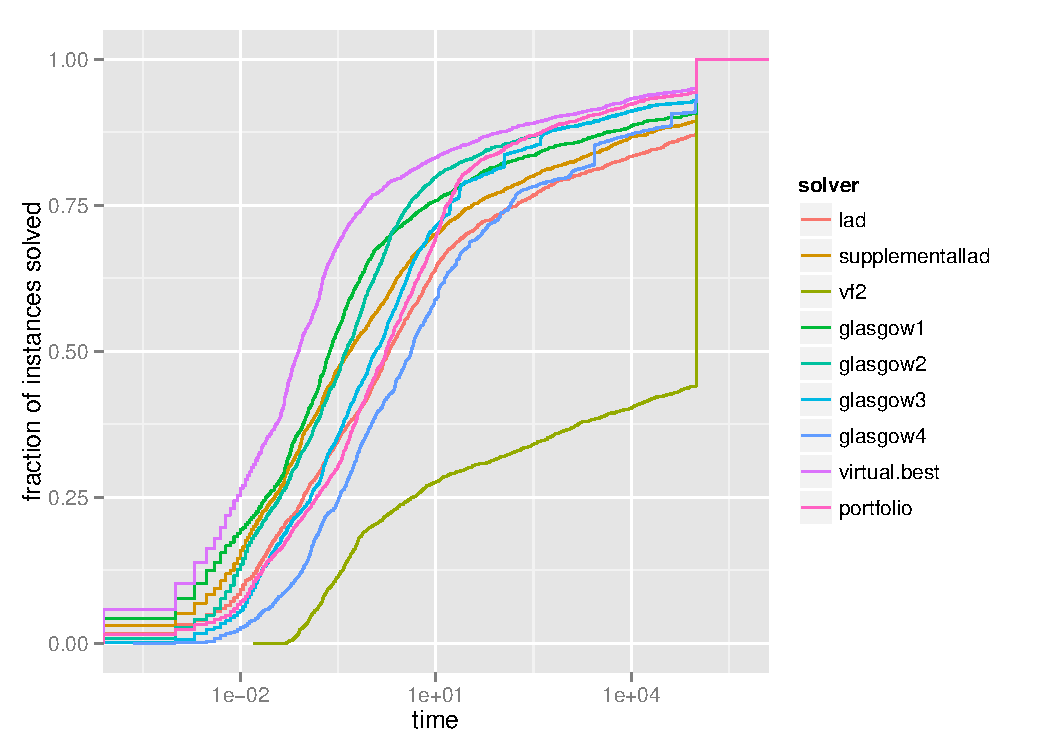
\includegraphics[width=\textwidth]{figures/portfolio-ecdf}
\caption{Number of solved instances over time for solvers, virtual best
solvers, and \LLAMA on the reduced set of 2336 instances. The
actual solvers are shown as dashed lines.}
\label{fig:portfolio-ecdf}
\end{figure}

Figure~\ref{fig:portfolio-ecdf-full} shows the number of solved instances over
time for the algorithm selection system including
\IncompleteLAD and \VFtwo presolving on the full set of instances. Note that for
very easy instances, we are better than the virtual best solver because
\IncompleteLAD is not included in our portfolio. The performance on small
instances is much better than the \LLAMA selector alone (cf.\
Figure~\ref{fig:portfolio-ecdf}) and the region where \LLAMA performs
worse than the individual solvers is now limited to approximately $10^2$ to
$10^5$ milliseconds.

\begin{figure}[!ht]
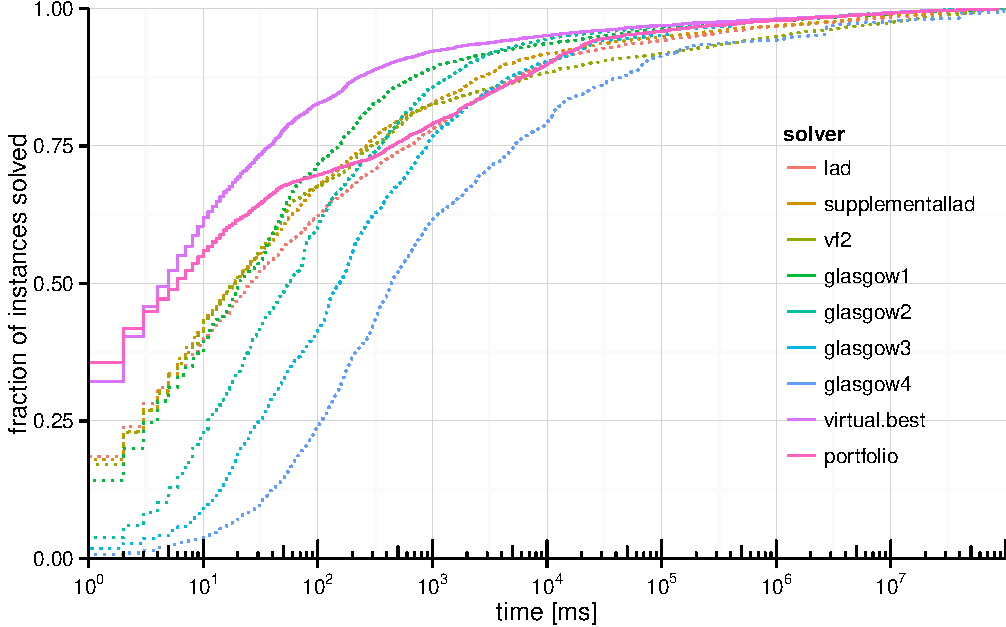
\includegraphics[width=\textwidth]{figures/portfolio-ecdf-full}
\caption{Number of solved instances over time for solvers, virtual best
solvers, and \LLAMA on the full set of 5725 instances. The
actual solvers are shown as dashed lines.}
\label{fig:portfolio-ecdf-full}
\end{figure}

We train the algorithm selection model specifically for the timeout of $10^8$
milliseconds. In particular, we are interested in minimising the performance
difference to the virtual best. Problem instances that take longer to solver
contribute more to this difference than easy instances and therefore carry more
weight for the algorithm selection model. That is, choosing the wrong solver for
a hard instances is much worse than choosing the wrong solver for an easy
instance.

Even though Figures~\ref{fig:portfolio-ecdf} and~\ref{fig:portfolio-ecdf-full}
show that on easy instances, the model does not perform well, it does over
the entire set of instances (cf.\ Tables~\ref{tab:res} and~\ref{tab:resfull}).

\subsection{Portfolios for Different Timeouts}

The question arises of whether the success of our approach is limited to the
particular timeout we have chosen. Table~\ref{tab:resTimeouts} shows the
performance of our algorithm selection approach for timeouts ranging from $10^2$
to $10^8$. We do not include the instances solved by \IncompleteLAD and \VFtwo
presolving here, as these components do not change for different timeouts.

\begin{table}[ht]
\centering
\begin{tabular}{llrrr}
  \toprule
timeout & solver & mean MCP & solved instances & mean performance\\
  \midrule
$10^2$ & virtual best & 0 & 1253 & 59\\
 & \LLAMA & 3 & 685 & 78\\
 & \GlasgowOne & 11 & 903 & 71\\
  \midrule
$10^3$ & virtual best & 0 & 1781 & 322\\
 & \LLAMA & 22 & 1284 & 569\\
 & \GlasgowOne & 126 & 1539 & 449\\
  \midrule
$10^4$ & virtual best & 0 & 1943 & 2018\\
 & \LLAMA & 186 & 1771 & 3342\\
 & \GlasgowTwo & 683 & 1855 & 2701\\
  \midrule
$10^5$ & virtual best & 0 & 2045 & 14348\\
 & \LLAMA & 1346 & 2022 & 17231\\
 & \GlasgowTwo & 3019 & 1988 & 17368\\
  \midrule
$10^6$ & virtual best & 0 & 2111 & 108060\\
 & \LLAMA & 10826 & 2087 & 120459\\
 & \GlasgowTwo & 22729 & 2063 & 130789\\
  \midrule
$10^7$ & virtual best & 0 & 2178 & 815577\\
 & \LLAMA & 91012 & 2156 & 908200\\
 & \GlasgowTwo & 198944 & 2129 & 1014522\\
  \midrule
$10^8$ & virtual best & 0 & 2219 & 5822809\\
 & \LLAMA & 740765 & 2204 & 6565232\\
 & \GlasgowTwo & 1969418 & 2172 & 7792227\\
\bottomrule
\end{tabular}
\vspace{1ex}
\caption{Algorithm selection performance for different timeouts.}\label{tab:resTimeouts}
\end{table}

The results show that while for the misclassification penalty, \LLAMA is always
better than the single best algorithm, for timeouts $10^2$ to $10^4$ it is worse
in terms of the number of solved instances and mean performance. The
misclassification penalty does not take the cost of computing features into
account, while the mean performance does---for these small timeouts, the cost
of computing the features dominates any improvement through algorithm selection.
Another explanation for this is that empirical runtime measurements are
inherently noisy, which affects the accuracy of the measurements and hence the
performance of the algorithm selection models particularly in this range.

\begin{table}[t]
\begin{center}
\begin{tabular}{|c||r||r|r|r||r|r|r|r||r|r|}
\hline
$t$ & \VFtwo & \multicolumn{3}{c||}{LAD} & \multicolumn{4}{c||}{\Glasgow}& VBS & $\delta$\\
&&incomplete&classic&path&1&2&3&4&&\\\hline
$10^0$ & 300 &  \cellcolor{blue!25}1126 & 661 & 599 & 386 & 95 & 39 & 12 & 1132 & 6\\\hline
$10^1$ & 1699 & 1858 & 2101 &  \cellcolor{blue!25}2287 & 2061 & 1215 & 455 & 208 & 3388 & 101\\\hline
$10^2$ & 2834 & 1912 & 3376 & 3708 &  \cellcolor{blue!25}3943 & 3344 & 2295 & 1329 & 4636 & 693\\\hline
$10^3$ & 3458 & 1918 & 4233 & 4531 &  \cellcolor{blue!25}4908 & 4763 & 4262 & 3426 & 5170 & 262\\\hline
$10^4$ & 3701 & 1919 & 4888 & 5025 & 5156 &  \cellcolor{blue!25}5253 & 5022 & 4408 & 5332 & 79\\\hline
$10^5$ & 3850 & 1919 & 5108 & 5193 & 5301 &  \cellcolor{blue!25}5377 & 5292 & 5082 & 5434 & 57\\\hline
$10^6$ & 3977 & 1919 & 5244 & 5307 & 5386 &  \cellcolor{blue!25}5452 & 5451 & 5235 & 5500 & 48\\\hline
$10^7$ & 4082 & 1919 & 5336 & 5414 & 5458 & 5517 &  \cellcolor{blue!25}5518 & 5425 & 5567 & 49\\\hline
$10^8$ & 4191 & 1919 & 5423 & 5479 & 5508 &  \cellcolor{blue!25}5561 & 5560 & 5554 & 5608 & 47\\\hline
\end{tabular}
\end{center}
\caption{Number of solved instances at different CPU time limits: Each line displays a time limit
$t$ (in milliseconds) followed by the number of instances solved within this time limit by \VFtwo,
\IncompleteLAD, classical \LAD, and \PathLAD, \Glasgow with the lengths of paths limited to 1, 2, 3 and
4, and the VBS. The best single algorithm is highlighted in blue, and the difference between VBS and
single best if displayed in the last column ($\delta$).\label{expTimeTable}}
\end{table}

Table~\ref{expTimeTable} displays the number of instances solved at different CPU time limits,
ranging from 1 to $10^8$ milliseconds. It shows us that the best single solver depends on the time
limit considered. Simple approaches like \IncompleteLAD and \VFtwo are able to solve easy instances
very quickly, in a few milliseconds. However, they are not able to solve harder instances:
\IncompleteLAD is an incomplete approach which can only detect rather trivial inconsistencies; \VFtwo
performs a basic backtracking search and is very fast on easy instances, because it does not compute
expensive invariants. Classical \LAD, \PathLAD, and the \Glasgow algorithms solve more instances than \VFtwo
and \IncompleteLAD when considering longer time limits: \SI{10}{\ms} for \LAD and \PathLAD and
\GlasgowOne, and \SI{100}{\ms} (resp. \SI{1000}{\ms} and \SI{10000}{\ms}) for \GlasgowTwo (resp.\ 3 and
4). The virtual best solver obtains much better results, showing us that the algorithms have complementary performance. The
difference between VBS and single best (column $\delta$ of Table \ref{expTimeTable}) is more
particularly important for rather small CPU time limits. In particular, VBS solves 693 more
instances than the single best (\GlasgowOne) when the limit is \SI{100}{\ms}. In many applications,
it is important to have the fastest possible algorithm. For example, in pattern recognition
applications, we often have to solve subgraph isomorphism problems for a very large number of graphs
(in order to find a pattern image in a large database of target images, for example), so that having
an algorithm that is able to solve an instance in \SI{100}{\ms} instead of \SI{1000}{\ms} makes a
big difference. Therefore, it is important to select the best algorithm for each instance.

Table~\ref{selectionvsvbs} shows the performance of our algorithm selection approach, compared to
the VBS (which is the upper bound of what an algorithm selection approach can achieve), and the
single best solver, at different CPU time limits (the single best corresponds to results highlighted
in blue in Table 1).  Comment Table 3: Mean runtime but also number of solved instances at different
CPU time limits.  Logically, \LLAMA may solve less instances than single best for small time limits
because it spends time to compute features and choose a solver, but it should be better for larger
time limits...

\begin{table}
\begin{tabular}{|l|r|rrrrrrrrr|}
&mean & \multicolumn{9}{c|}{Number of solved instances}\\
&runtime & $10^0$ &  $10^1$ &  $10^2$ &  $10^3$ &  $10^4$ &  $10^5$ &  $10^6$ &  $10^7$ &  $10^8$\\\hline
VBS & 2375.9 & 1132 & 3388 & 4636 & 5170 & 5332 & 5434 & 5500 & 5567 & 5608\\\hline
Single best & 3177.6 & 1126 & 2287 & 3943 & 4908 & 5253 & 5377 & 5452 & 5518 & 5561\\\hline
\LLAMA & 2706.3\\\hline
\end{tabular}
\caption{}\label{selectionvsvbs}
\end{table}

Add Figure 1 which compares single best at \SI{e8}{\ms}(\GlasgowTwo) with \LLAMA ?

\section{Conclusion and Future Work}\label{sec:concs}

The problem of identifying subgraph isomorphisms is a hard computation problem
that has many applications in diverse areas. In this paper, we presented a
portfolio of six algorithms from the literature and a novel variant of the \LAD
algorithm. We introduced a
set of novel features to characterise subgraph isomorphism problems and
leveraged them to select the most appropriate algorithm from the portfolio for
each instance.

We demonstrated that our algorithm selection approach achieves substantial
performance improvements over the single algorithm that has the best performance
on our benchmark set. We showed that combining an algorithm selection approach
with a novel incomplete variant of \LAD that is able to detect inconsistencies
and a presolver boosts performance even further.

Mention parallel, directed, labelled in here briefly.

\bibliographystyle{splncs}
\bibliography{paper}

\end{document}
